%\documentstyle[11pt,thesis,diagram,tgrind]{uuthesis}
\documentclass[Chicago]{uuthesis2e}
%\includeonly{ch3,ch4,ch6,ch5}%  % BEWARE: First % kills white space
%\includeonly{ch4,ch5,ch6}%  % BEWARE: First % kills white space
%\includeonly{ch1,ch2,ch3,ch4,ch5,ch6}%  % BEWARE: First % kills white space
%\includeonly{ch1,ch2,ch3}
%\RequirePackage{times}
%\RequirePackage{algorithmic}
%\PassOptionsToPackage{boxed}{algorithm}
%\RequirePackage{algorithm}
%\RequirePackage{pseudocode}
%% Algorithm
\usepackage
{
    cite, 
    epsfig,
    epstopdf, 
    graphicx, 
    color, 
    float,
    subfig,
    amssymb,
    xspace,
    tabularx,
    rotating,
    lscape,
    afterpage,
    url,
    listings,
    multirow,
    hhline,
    placeins
} 

\usepackage{amsmath}
\usepackage{algorithmic}
\renewcommand{\algorithmicrequire}{\textbf{Input:}}
\renewcommand{\algorithmicensure}{\textbf{Output:}}

\usepackage{polynom}
\usepackage{blkarray}
\usepackage{enumerate}

\usepackage[ruled]{./algorithm2e}
%%for algorithm2e package, label has to be following caption in the same line!!!

\RequirePackage{times}


\def\BibTeX{{\rm B\kern-.05em{\sc i\kern-.025em b}\kern-.08em
    T\kern-.1667em\lower.7ex\hbox{E}\kern-.125emX}}


\setcounter{page}{1}

% New command for the table notes.
\def\tabnote#1{{\small{#1}}}

% New command for the line spacing.
\newcommand{\ls}[1]
    {\dimen0=\fontdimen6\the\font
     \lineskip=#1\dimen0
     \advance\lineskip.5\fontdimen5\the\font
     \advance\lineskip-\dimen0
     \lineskiplimit=.9\lineskip
     \baselineskip=\lineskip
     \advance\baselineskip\dimen0
     \normallineskip\lineskip
     \normallineskiplimit\lineskiplimit
     \normalbaselineskip\baselineskip
     \ignorespaces
    }

\newcommand{\beq}{\begin{equation}}
\newcommand{\eeq}{\end{equation}}
\newcommand{\ov}{\bar}
\newcommand{\xor}{\bigoplus}
%\newtheorem{definition}{Definition}[section]
\newcommand{\beqarr}{\begin{eqnarray}}
\newcommand{\eeqarr}{\end{eqnarray}}
\newcommand{\tab}{\xspace\ \ \ \ \xspace}
\newcommand{\ttab}{\xspace\ \ \xspace}

\newcommand{\eqntext}[1]{\text{\xspace\rm #1\xspace}}

\newcommand{\Fq}{{\mathbb{F}}_{q}}
\newcommand{\Fp}{{\mathbb{F}}_{p}}
\newcommand{\Fpk}{{\mathbb{F}}_{p^k}}
\newcommand{\Fkk}{{\mathbb{F}}_{2^k}}
\newcommand{\Z}{{\mathbb{Z}}}
\newcommand{\Zkk}{{\mathbb{Z}}_{2^k}}
\newcommand{\Fkkx}[1][x]{\ensuremath{\mathbb{F}}_{2^k}[#1]\xspace}
\newcommand{\Grobner}{Gr\"{o}bner\xspace}
%\newcommand{\Grobner}{Gr\"{o}bner}
\newcommand{\bi}{\begin{itemize}}
\newcommand{\ei}{\end{itemize}}
\newcommand{\Func}{{\mathcal{F}}}
\newcommand{\N}{{\mathcal{N}}}
\newcommand{\G}{{\mathcal{G}}}
\newcommand{\F}{{\mathbb{F}}}
\newcommand{\B}{{\mathbb{B}}}
\newcommand{\C}{{\mathbb{C}}}
\newcommand{\R}{{\mathbb{R}}}
\newcommand{\K}{{\mathbb{K}}}
\newcommand{\M}{{|\bf M}|}
\newcommand{\Mi}{{|\bf M_i|}}

\newtheorem{Theorem}{Theorem}[chapter]
\newtheorem{Definition}{Definition}[chapter]
\newtheorem{Example}{Example}[chapter]
\newtheorem{Proposition}{Proposition}[chapter]
\newtheorem{Lemma}{Lemma}[chapter]
\newtheorem{Corollary}{Corollary}[chapter]
\newtheorem{Conjecture}{Conjecture}[chapter]
\newtheorem{Problem}{Problem\ Setup}[chapter]

%\newtheorem{Proof}{Proof}[chapter]
%%%%%%%%%%%%%%%%%%%%%%%%%%%%%%%%%%%%%%%%%%%%%%%%%%%%%%%%%%%%%%%%%%%%%%%%

%\title{Word-Level Polynomial Abstraction of Galois Field Circuits using Gr\"obner Bases} 
\title{Word-level Techniques for Abstraction and Verification of Sequential Circuits using Algebraic Geometry}
\author{Xiaojun Sun} 
\thesistype{dissertation}
\degree{Doctor of Philosophy}

%%%%%%%%%%%%%%%%%%%%%%%%%%%%%%%%%%%%%%%%%%%%%%%%%%%%%%%%%%%%%%%%%%%%%%%%

\chairtitle{Professor}
\committeechair{Priyank Kalla}
\firstreader{Ganesh Gopalakrishnan}
\secondreader{Chris J. Myers}
\thirdreader{Kenneth S. Stevens}
\fourthreader{Rongrong Chen}
\graduatedean{David B. Kieda}
\department{Department of Electrical and Computer Engineering}
\departmentchair{Gianluca Lazzi}

\submitdate{Dec 2016}
\copyrightyear{2016}
\dedication{}

%%%%%%%%%%%%%%%%%%%%%%%%%%%%%%%%%%%%%%%%%%%%%%%%%%%%%%%%%%%%%%%%%%%%%%%%
\fourlevels

%\input{BoxedEPS.tex}
%\input{epsf}


\begin{document}
%\ls{1.5}
%\linespread{0.9}
%%%%%%%%%%%%%%%%%%%%%%%%%%%%%%%%%%%%%%%%%%%%%%%%%%%%%%%%%%%%%%%%%%%%%%%%

\frontmatterformat
%\setcounter{page}{1}
\titlepage
\copyrightpage
\committeeapproval
\readingapproval

%\preface{abstract}{Abstract}
%\dedicationpage
\tableofcontents
\listoffigures
\listoftables

%%%%%%%%%%%%%%%%%%%%%%%%%%%%%%%%%%%%%%%%%%%%%%%%%%%%%%%%%%%%%%%%%%%%%%%%

%\preface{acknowledge}{Acknowledgements}
\maintext       % Start normal page numbering. Parts and chapters follow.

\begin{center}{\bf ABSTRACT}\end{center}
Formal verification of hardware designs has become an essential
component of the overall system design flow. The designs are generally
modeled as finite state machines, on which property and equivalence
checking problems are solved for verification. Reachability analysis
forms the core of these techniques. However, increasing
size and complexity of the circuits causes the state explosion
problem. Abstraction is key to tackle the scalability challenge.

This dissertation presents new techniques for word-level abstraction
with applications in sequential design verification. By bundling
together $k$ bit-level state-variables into one word-level constraint 
expression, the state-space is construed as solutions (variety) to
a set of polynomial constraints (ideal), modeled over the finite
(Galois) field of $2^k$ elements. Subsequently, techniques from
algebraic geometry -- notably, Gr\"obner basis theory and technology
-- are researched to perform reachability analysis and
verification of sequential circuits. This approach adds a ``word-level
dimension'' to state-space abstraction and verification to make the
process more efficient.

While algebraic geometry provides powerful abstraction and reasoning
capabilities, the algorithms exhibit high computational complexity. In
the dissertation, we show that by analyzing the constraints, it is
possible to obtain more insights about the polynomial ideals, which can be
exploited to overcome the complexity. Using our algorithm design and
implementations, we demonstrate how to perform reachability
analysis of finite-state machines purely at the word-level. Using this
concept, we perform scalable verification of sequential arithmetic
circuits. As contemporary approaches make use of resolution proofs and
unsatisfiable cores for state-space abstraction, we introduce the
algebraic geometry analog of unsatisfiable cores, and present
algorithms to extract and refine unsatisfiable cores of polynomial
ideals. Experiments are performed to demonstrate the efficacy of our
approaches. 

\chapter{Introduction} \label{ch:intro}
There is an ever-increasing need for secure communication within information 
technology. Security of sensitive information relies more and more heavily 
on encryption methodologies implemented in hardware by cryptographic 
circuits. One of the most prominent of these methodologies is Elliptical 
Curve Cryptography (\emph{ECC}), which provides more strength per encryption bit 
than other encryption methodologies.
The main building blocks of ECC hardware implementations 
are fast, \emph{custom-built Galois field arithmetic circuits}.
These circuits are notoriously hard to verify, yet their correctness is 
vitally important in critical applications. In \cite{crypto:bug_attacks}, 
for example, it is shown that a bug in the hardware could lead to the full 
leakage of the secret cryptographic key, which could compromise the entire
system. Thus, formal verification is imperative in Electronic Design 
Automation (\emph{EDA}) when dealing with cryptographic circuits.

To facilitate this verification, it is highly desirable to obtain a {\it word-level 
representation of the datapath of the ECC arithmetic block} from its 
bit-level implementation. Ideally, this abstraction should be {\it canonical},
as this allows the it to be directly applicable to equivalence checking. 
Such a canonical, word-level abstraction of the 
Galois field arithmetic block would not only make it easier to verify and 
reason 
about the cryptographic system as a whole, but also enable the use of 
higher level abstraction and synthesis tools. 
As arithmetic circuits are custom-designed, often modularly, using Galois field arithmetic blocks, 
the abstraction should also exploit the hierarchical nature of the circuitry.
Due to the modular circuit structure, abstraction of each arithmetic block
becomes the key in verification of the full circuit. 
Practical 
applications of ECC dictate a datapath of a minimum of $163$-bits, up to 
$571$-bits, as 
designated by the National Institute for Standards and Technology (NIST).
However abstraction of 
Galois field arithmetic circuits has been infeasible for data-paths beyond 
$16$ bits. 

This dissertation proposes an algebraic geometry based approach to abstract canonical, 
word-level representations of bit-level Galois field arithmetic circuits.
The approach is able to abstract representations
for circuits up to 571 bits in size, which is the largest NIST
standard for datapath size in ECC. 
Verification of circuits for which this abstraction has been computed is shown to 
be trivial; thus, the focus is on deriving the abstraction quickly and efficiently.
%Furthermore, we show how we can use these abstract representations to 
%perform improved formal verification of these circuits.

\section{Hardware Design and Verification Overview}
The typical design flow of a hardware system, 
as shown in Fig. \ref{fig:cadflow}, starts with a hardware system 
specification, which describes the necessary functions and parameters that 
the system must perform and adhere to. The specification is typically
modelled using a transaction-level model (\emph{TLM}), which describes 
communication details between large circuit modules. 
The TLM is then translated 
into a register-transfer-level (\emph{RTL}) description, which is composed of abstracted, 
interconnected circuit blocks that compose the entire system. RTL is 
typically implemented 
in hardware description languages (\emph{HDL}) such as Verilog and VHDL, 
which are the most popular choices in the industry.
Next, the RTL is optimized and converted into a \emph{netlist}, i.e. a large 
collection of small physical blocks (MOSFET, Boolean logic gates, etc.) and 
the inter-connections (wires) between them. 
Lastly, the netlist is further optimized and then mapped onto a physical space 
on a chip, which is then sent off for fabrication. This entire design flow
is automated by Computer-Aided Design (\emph{CAD}) tools. 

{
\begin{figure}[h]
\centerline{
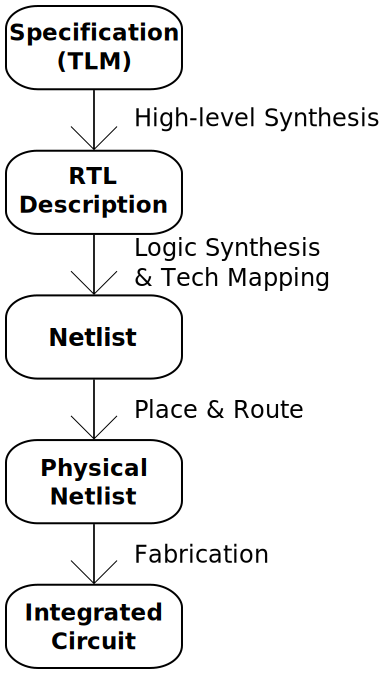
\includegraphics[width=0.5\textwidth]{./figures/designFlow}
}
\caption{Typical hardware design flow.}
\label{fig:cadflow}
\end{figure}
}

%\subsection{The Hardware Verification Imperative}
When moving from one abstraction level of the hardware design process to the 
next, an important issue arises: how can one ensure that the functionality of 
the optimized design matches original spec? 
Bugs in hardware design which are 
not caught early can have costly effects later, such as the need for a 
redesign. Bugs in arithmetic circuits can be especially catastrophic.
One infamous example is the 1994 floating point division (FDIV)
bug that affected the Intel Pentium chip \cite{nicely:FDIV}, 
and subsequently cost the company \$475 million because it was  
discovered after the chip's release. In another more fatal case, during the
Gulf war, an American Patriot Missile battery failed to intercept an incoming
enemy missile due to an arithmetic error \cite{arnold:patriot}.
Since hardware bugs can have significant consequences, 
there has been extensive work in field of hardware verification to find and
eliminate bugs prior to fabrication.

The two main methodologies used in hardware verification are simulation and 
formal verification. \emph{Simulation} checks correctness by applying exhaustive 
assignments to the circuit inputs and verifying correctness of the output. 
This ensures that the circuit performs as designed under all possible 
inputs. Such exhaustive testing is quite effective for smaller circuits. 
However, as the size of the circuit increases, it becomes 
computationally infeasible to simulate all possible test vectors. This is the 
case with Galois field arithmetic circuits, which are commonly very large in 
real-world applications. Often for such large circuits, simulations of a smaller and more 
manageable subset of test vectors are employed to catch bugs. While these tests
can increase confidence in the correctness of the design,  
{\it they do not guarantee correctness} since every data-flow of the design hasn't
been analyzed.
%Such is the case with large Galois field arithmetic circuits, so we instead 
%focus on formal verification. 

\section{Formal Verification}
Instead of simulating input vectors, \emph{formal verification} utilizes 
mathematical theory to reason about the correctness of hardware designs.
%which overcomes some limitations of simulation. 
Formal verification has two main forms: property checking and equivalence 
checking. 

{\it Property checking} (or property verification) verifies
that a design satisfies certain given properties. Property checking is done mainly 
in the form of theorem proving, model checking, or approaches which 
combine the two.
\begin{enumerate}
\item \emph{Theorem proving} \cite{theoremproving:91} requires the existence of
mathematical descriptors of the specification and implementation of the 
circuit. Theorem provers apply mathematical rules to these descriptors to
derive new properties of the specification. In this way, the tool can reduce
a proof goal to simpler sub-goals, which can be automatically verified.
However, generating the initial proof-goal requires extensive guidance from
the user, so there is an overall lack of automation in theorem 
proving.
\item \emph{Model checking} \cite{modelcheck:99} is an approach
to verifying finite-state systems where specification 
properties are modeled as a system of 
logic formulas. The design is then traversed to check if the 
properties hold. If the design is found to violate a
particular property, a counter-example is generated which exercises the
incorrect behavior in the design. Such counter-examples allow the designer
to trace the behavior and find where the error in the design lies.
Modern model checking techniques use the result to automatically refine
the system and perform further checking.
These tools are typically automated, and thus have found widespread 
use in CAD tool suites.
\end{enumerate}

{\it Equivalence Checking} verifies that two different representations of
a circuit design have equivalent functionality. An example of equivalence
checking as it applies to the hardware design flow is shown in
Fig. \ref{fig:equivflow}.

{
\begin{figure}[h]
\centerline{
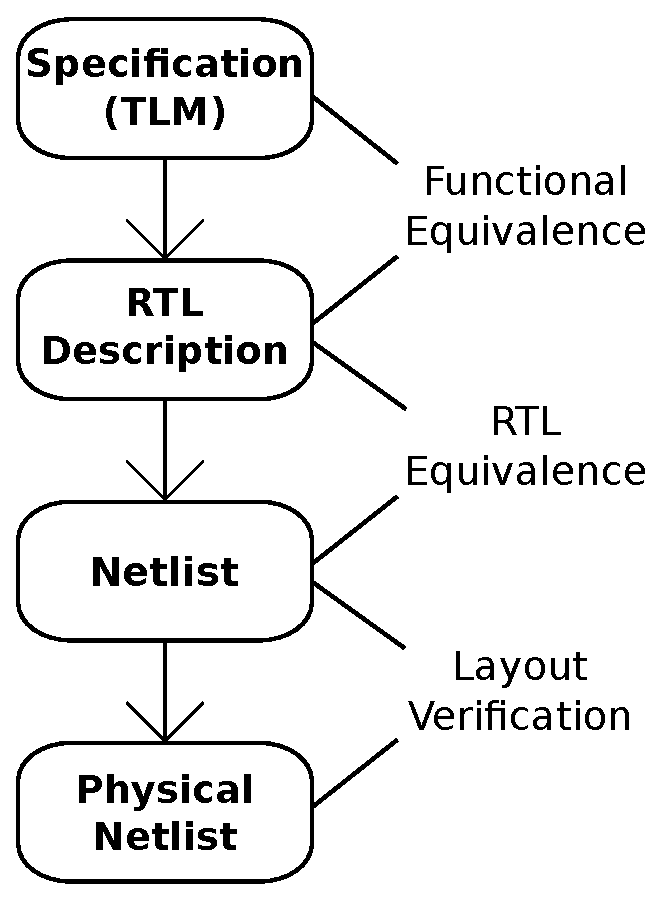
\includegraphics[width=0.5\textwidth]{./figures/designVerification}
}
\caption{Equivalence checking as applied to the hardware design flow.}
\label{fig:equivflow}
\end{figure}
}

There are two major
equivalence checking techniques: graph-based
and satisfiability-based.
\begin{enumerate}
\item \emph{Graph-based} techniques construct a canonical graph 
representation, such as a Binary Decision Diagram (\emph{BDD}) or one of
its many variants, of each circuit. A linear comparison is then conducted to 
determine whether the two graphs are isomorphic. Since the graph 
representation is canonical, the graphs of the two circuits will be 
equivalent if and only if the circuits perform the same function.
\item \emph{Satisfiability} techniques construct a miter of the two circuits,
typically in a graph such as an And-Inverter graph (\emph{AIG}). A
\emph{miter} is a combination of the two circuits with one bit-level output, which 
is only in a "1" state when the outputs of the circuits differ given 
the same given 
input, as shown in Fig. \ref{fig:miter}. 
A satisfiability (\emph{SAT}) tool \cite{csat} 
is then employed to simplify the graph and find a solution to the miter, 
i.e. find an input for which the 
miter output is "1". If a solution is found, this solution acts as a 
counter-example of when the circuit outputs differ; otherwise the circuits
are functionally equivalent.
\end{enumerate}


{
\begin{figure}[h]
\centerline{
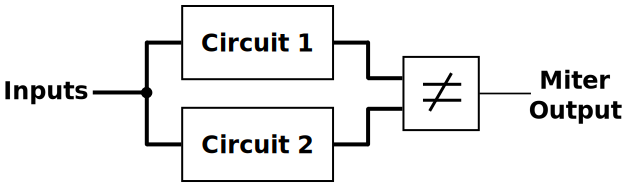
\includegraphics[width=0.8\textwidth]{./figures/betterMiter}
}
\caption{A miter of two circuits.}
\label{fig:miter}
\end{figure}
}

%\subsection{Computer-Algebra Based Formal Verification}
Certain formal verification methods use \emph{computer-algebra} and \emph{algebraic
geometry} techniques based on mathematical theories.
Unlike SAT-based verification, modern algebraic geometry 
techniques do not explicitly solve the constraints to find a solution; 
rather, they reason about the presence or absence of solutions, or explore
the geometry of the solutions.
These methods \cite{Avrunin:CAV} \cite{condrat-tacas07} \cite{gbverify:2007} 
transform the circuit design into a polynomial system. Typically, this system
of polynomials is then used to compute a Gr\"obner basis \cite{gb_book}. 
Computation of Gr\"obner bases allows for 
the easy deduction of important properties of a polynomial system, 
such as the presence or absence of 
solutions. These properties are then leveraged to perform 
verification. Unfortunately, such a computation 
has been shown to be doubly 
exponential in the worst case, and thus these methods have not been 
practical for real-world applications. However, recent
breakthroughs in computer-algebra hardware verification have shown
that it is possible to overcome the complexity of this computation while
still utilizing the beneficial properties of a Gr\"obner bases
\cite{lv:phd}.

\section{Importance of Word-level Abstraction}
Most formal verification techniques can benefit from word-level abstractions 
of the circuits they verify.
Abstraction is defined as state-space reduction, i.e{\text . }abstraction
reduces state-space by mapping the set of states of a system to a smaller 
set of states. Because the new representation contains fewer states, it
is easier to comprehend and thus easier to use. 
Word-level abstraction focuses specifically on abstracting a word-level
representation of a circuit out of a bit-level representation. For example,
a bit-level representation of an integer multiplier is represented by a
collection of Boolean inputs and outputs, whereas a word-level
abstraction hides the underlying logic and represents the circuit as two 
integer inputs and one integer output, e.g. $Z=A\cdot B$. As the bit-size of the
multiplier increases, the logical implementation of the multiplier grows (typically
exponentially) while the word-level abstraction stays the same.

Word-level abstractions have a wide variety applications in formal 
verification. Theorem proving techniques can leverage abstraction as an 
automatic decision procedure or as a canonical reduction 
engine. For example, since RTL is composed of circuit blocks that represent 
the underlying circuit, RTL verification methods can exploit 
abstractions of these blocks.
This is seen in the following RTL verification methods:
\begin{itemize}  
\item Model checking \cite{kroening:model}, 
where an approximation abstraction of RTL blocks is generated and then 
refined.
\item Graph-based equivalence 
checking \cite{WLS} \cite{arditi:bmd}, where abstraction methods are used
to generate a canonical word-level graph representation of the circuit.
\item Satisfiability-based equivalence checking \cite{lpsat}, where 
abstractions are used identify symmetrics and similarities in order to 
minimize the amount of logic that is sent to the 
SAT tool. 
\end{itemize}

Other equivalence checking techniques that employ abstractions 
include satisfiability modulo theory ({\it SMT}) techniques \cite{boolector} \cite{bryant:tacas07}, 
which are similar to SAT except they operate on higher-level data
structures (integers, reals, bit vectors, etc.), as well as 
constraint solving techniques \cite {ms:research} \cite{tew:iccad08}.
In general, RTL equivalence checking approaches would ideally maintain a 
high-level of abstraction while still retaining sufficient lower-level 
functional details  (such as bit-vector size, precision, etc) 
\cite{gupta_survey}.

Word-level hardware abstractions also have applications in RTL and datapath 
synthesis \cite{demicheli:iccad_98} \cite{demicheli:dac_99}
\cite{demicheli:tcad_03}. 
Abstractions of circuits allow for design reuse, which allows for tool-automated 
synthesis of larger circuit blocks.
Since hardware design specifications tend to be word-level, synthesis tools 
can use these larger circuit blocks to generate and optimize the
datapaths and create the RTL of the system. Thus, in order for a circuit to 
be used by these automated synthesis tools, its word-level abstraction must
be known.

Finally, abstractions can also be applied to detect malicious 
modifications to a circuit, potentially inserted as a hardware trojan horse.
Hardware trojans, a relatively new security concern in the hardware 
industry, use certain techniques to add incorrect behavior to a 
design. 
This behavior is only activated under certain rare circumstances that only 
the mal-intent designer has knowledge of.
The behavior is purposely hidden and is very difficult to encounter during 
simulation of the design. A manufactured chip with a subsystem 
that contains a hardware trojan could compromise the entire system in which 
it is used.
In some hardware trojan cases, formal verification techniques may be applied 
to catch a bug in a design and provide a counter-example which exercises it. 
However, it can be difficult to tell whether the bug in the design was 
introduced intentionally of not. On the other hand, word-level abstractions 
of bit-level circuits {\it effectively reverse-engineer the true function 
implemented by the circuit}, which could be used to determine the designer's 
true intention.

\section{Dissertation Objective, Motivation, and Contributions}
This dissertation focuses on abstracting a canonical, 
word-level representation of hardware (bit-level) implementations of 
combinational circuits. The proposed technique is a full abstraction solution which can be 
applied to any arbitrary acyclic combinational circuit. 
It is particularly efficient when applied to Galois field arithmetic circuits.
Using this technique, if the abstraction of the circuit's implementation and its
specification are found, they can be easily compared to determine equivalence.
Implementation of a custom software tool, developed to compute the abstractions, is
also described.

\subsection{Motivating Application}
The motivation for this work comes from applications of Galois field 
arithmetic circuits in elliptical curve cryptography ({\it ECC}) hardware systems.
The main operations of encryption, decryption, and 
authentication in ECC rely on operations performed on elliptic curves, which 
are implemented in hardware as polynomial functions over Galois fields. 
To be applicable in real-world situations, ECC data-paths
should be a minimum of $163$-bits wide, which is the minimum NIST standard, 
up to a recommended size of $571$-bit operand widths. Many non-ECC cryptosystems
have datapaths on the order of $1000$-bits.

A Galois field arithmetic circuit with a datapath size of $k$ 
is built as a Boolean function: $\mathbb{B}^k \rightarrow \mathbb{B}^k$. 
This function is mapped to an operation 
$f:\mathbb{F}_{2^k} \rightarrow \mathbb{F}_{2^k}$ 
over the Galois field $\mathbb{F}_{2^k}$. 
These circuits are custom-built, modular
systems which cannot be synthesized due to their complex nature. Thus, 
formal verification is needed to ensure they operate correctly.

Recent computer-algebra based formal verification techniques have been
able to perform verification of Galois field arithmetic circuits with
a datapath size up to $163$-bits \cite{lv:phd}. Word-level abstractions 
of Galois
field arithmetic circuits could be used to further improve these formal 
verification techniques to allow for verification of larger circuits, as
well as provide the other benefits of word-level abstraction.
However, there is currently no technique for computing word-level 
abstractions of Galois field circuits of any practical size.

{
\begin{figure}[h]
\centerline{
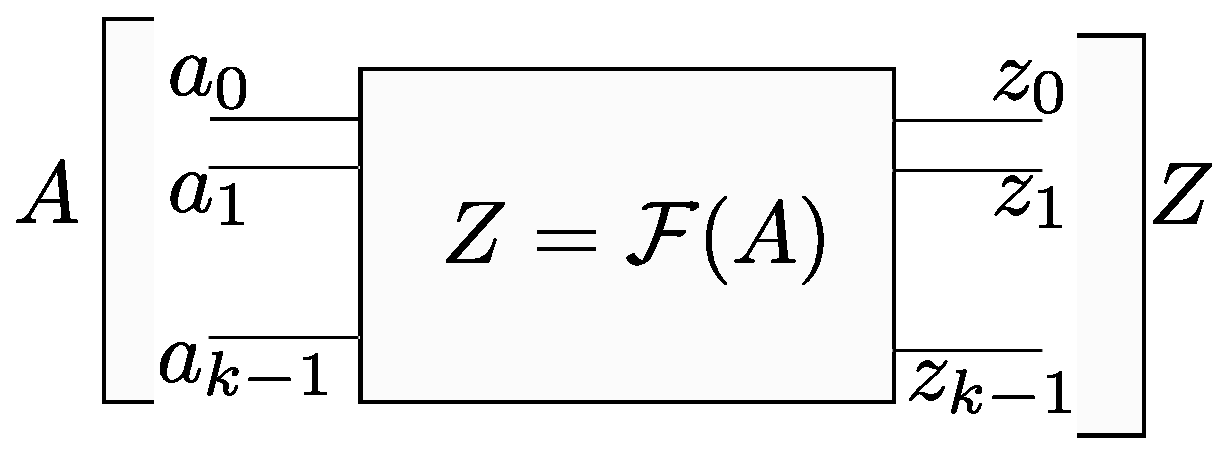
\includegraphics[width=0.5\textwidth]{./figures/interpolate}
}
\caption{Circuit with $k$-bit input $A$ and $k$-bit output $Z$. 
Abstraction to be derived as $Z=\Func(A)$.}
\label{fig:abstractA_Z}
\end{figure}
}

While the motivation comes from the need to verify Galois field arithmetic
circuits, the presented approach can be generalized to be applicable to any
combinational acyclic circuit.
Any such circuit with a $k$-bit input $A$ and a $k$-bit output $Z$, such
as the one shown in Fig. \ref{fig:abstractA_Z}, computes 
$f: \mathbb{B}^k \rightarrow \mathbb{B}^k$ and can thus be analyzed as the
function $f: \Fkk \rightarrow \Fkk$. Over $\Fkk$ this function can be 
represented as the polynomial $Z=\Func(A)$. This is trivially generalized
when there are multiple $k$-bit inputs $A_1,A_2,\dots,A_i$, i.e. $Z=\Func(A_1,\dots,A_i)$.
Now assume the word-size of the input differs from the output, that is the circuit
computes $f: \mathbb{B}^m \rightarrow \mathbb{B}^n$ for $m \neq n$. This can 
be represented as a function over Galois fields as $f: \F_{2^m} \rightarrow \F_{2^n}$.
This function can be analyzed over the field $\Fkk$ such that $\Fkk \supset \F_{2^m}$ 
and $\Fkk \supset \F_{2^m}$, where $k=LCM(m,n)$.

\subsection{Dissertation Contributions}
To solve the problem of word-level abstraction, this dissertation proposes 
a full solution consisting of three main contributions.

\begin{enumerate}
\item A theory for finding the word-level abstraction from a bit-level circuit over Galois fields is created.
The given bit-level circuit implementation is modelled as a system of
polynomials over the field.
This theory is derived using techniques from computer-algebra, notably the theory of
\Grobner basis \cite{pruss:iwls13}.
\item Using this theory, new algorithms based on symbolic computation are developed to 
derive the word-level abstraction. The algorithms are designed to be applicable to 
industry-size arithmetic circuits over Galois fields \cite{pruss:dac14}\cite{sun:date15}.
A complexity analysis of the algorithmic approach is also presented. Furthermore, the
approach is also generalized to make it applicable to arbitrary combinational circuits.
Finally, we show how the approach can be used to exploit the hierarchical structure of
large Galois field multipliers designed over composite fields.
\item A custom software tool implementation of the algorithmic approach is described, including
an analysis of efficient data structures designed for this purpose \cite{pruss:tcad15}.
\end{enumerate}

Experiments show that the proposed solution can abstract canonical, word-level, 
polynomial representations of Galois field arithmetic circuits up to $1024$-bits in
size, while other contemporary approaches are infeasible beyond a $32$-bit designs.


%an 
%approach based on computer-algebra, algebraic geometry - notably the theory of
%{\it Gr\"obner bases} \cite{gb_book} \cite{buchberger_thesis}.
%and {\it elimination ideals} \cite{ideals:book}, as our approach for 
%abstracting canonical word-level representations from bit-level Galois 
%field arithmetic circuits. 
%Computer-algebra techniques easily integrate with 
%Galois field theory and allow for polynomial abstraction of the circuit over 
%the field itself. Thus, if the circuit computes a function over some field $
%\mathbb{F}_{2^k}$, the resulting abstraction is a word-level polynomial 
%function over the same field $\mathbb{F}_{2^k}$. 

%The given bit-level circuit implementation is first modeled as a system of
%polynomials over the field. Using the theory of elimination ideals, we 
%derive an elimination term ordering and prove that by using this ordering we 
%can obtain a canonical word-level representation of a circuit by 
%computing a Gr\"obner basis of the polynomials. However, complexity 
%of the computation of a Gr\"obner basis proves to be prohibitive for circuits
%of practical size. Therefore, we employ a select sub-set of computations 
%from the Gr\"obner basis theory to overcome this complexity and obtain the
%abstraction. We prove that this simpler computation can be 
%performed via a polynomial reduction process, and engineer a custom 
%verification tool for this purpose. Using this approach, we are able to 
%successfully 
%abstract word-level representations of Galois field arithmetic circuits up 
%to $571$-bits, which is the {\it largest recommended NIST standard} for ECC.


\section{Dissertation Organization}
The rest of this dissertation is organized as follows. Chapter
\ref{ch:prev} reviews previous applicable work and highlights their
drawbacks with respect to the canonical, word-level abstraction problem. 
Chapter \ref{ch:prelim} describes the properties of Galois fields, 
$\mathbb{F}_{2^k}$, and explains the process of constructing them.
It also describes how to design arithmetic circuits over such fields, their 
complexities, and the role of these circuits in Elliptic Curve Cryptography.
Chapter \ref{ch:ideals} provides a theoretical background of 
computer-algebra and Gr\"obner bases and explains their application
to Galois fields. 
Chapter \ref{ch:abstract} describes an approach to abstract 
word-level polynomial representations of combinational circuits using a 
Gr\"obner basis computation.
Chapter \ref{ch:improv} improves on this word-level abstraction approach to 
make it applicable to much larger circuits.
Chapter \ref{ch:generalize} generalizes the abstraction approach to make
it applicable to circuits with varying operand word-lengths. It also describes how the 
approach can take advantage of the hierarchy of arithmetic circuits designed over
composite fields.
Chapter \ref{ch:implement} describes the implementation details of a 
custom abstraction tool and gives experimental results of
abstracting large Galois field multiplier circuits.
Chapter \ref{ch:concl} concludes the dissertation and outlines potential future 
research for continuation of this work. 

\chapter{Previous Work}
\label{ch:prev}
\vspace{-0.8cm}
\section{Sequential Equivalence Checking}
As an important component of formal verification for sequential circuits, SEC techniques 
have been developed over decades and widely utilized in both academia and industry. 
The specification of a sequential circuit can be modeled as a (golden model) state machine;
SEC is performed to compare the functionality between the circuit for test and the golden one.
% The n\"aive method to implement SEC is: preload both circuits to the same initial states, 
% and assign their primary inputs to the same values during all clock-cycles.
% This method needs to be operated along with state space traversal,  therefore it is 
% less efficient. Moreover,  most SEC only check the primary outputs/inputs consistency 
% and does not require the 1:1 state correspondence,  so state space traversal is not always necessary.
One way to implement SEC is to create a miter with two circuits to be verified, then 
prove that there exists no sequence of inputs that generates different outputs.

Researchers proposed improvements by using Boolean functions to represent 
a set of states/transitions \cite{coudert2003unified, coudert1990verification},  or by dividing the sequential circuit
into a smaller subcircuit and remodeling the FSM to conditional FSMs \cite{khasidashvili2004theoretical}. IBM created a toolset with 
interfaces that focuses on only the designated initial states and removes redundancies in state space \cite{baumgartner2007scalable}.

Another direction to improve SEC algorithms is to avoid using state space traversal. 
The forward retiming method \cite{van1998sequential} and time-frame merging \cite{stoffel1997record} 
all work on an array of time-frames,  with the assistance of combinational equivalence checking (CEC)
techniques. These techniques require structural similarities between the two circuits.

The most significant difference of sequential circuits from combinational circuits is 
that the outputs of the circuit depend not only 
on the primary inputs, but also on current state. 
The behavioral difference reflects on the structural design of circuits and in 
the existence of memory components such as latches and flip-flops.
In order to test certain properties on some signals across multiple clock-cycles,
the most straightforward method is to propagate those signals throughout 
all clock-cycles. Moreover, for formal verification, all signals on all paths from the circuit
need to be propagated through multiple clock-cycles.
This indicates a time-to-space conversion, where 
 the combinational part of circuit
is copied over several time-frames then connected together.
The procedure is called {\it unrolling} of a sequential circuit, as 
Figure \ref{fig:unrolling} shows.

\begin{figure}[tbp]
\centerline{
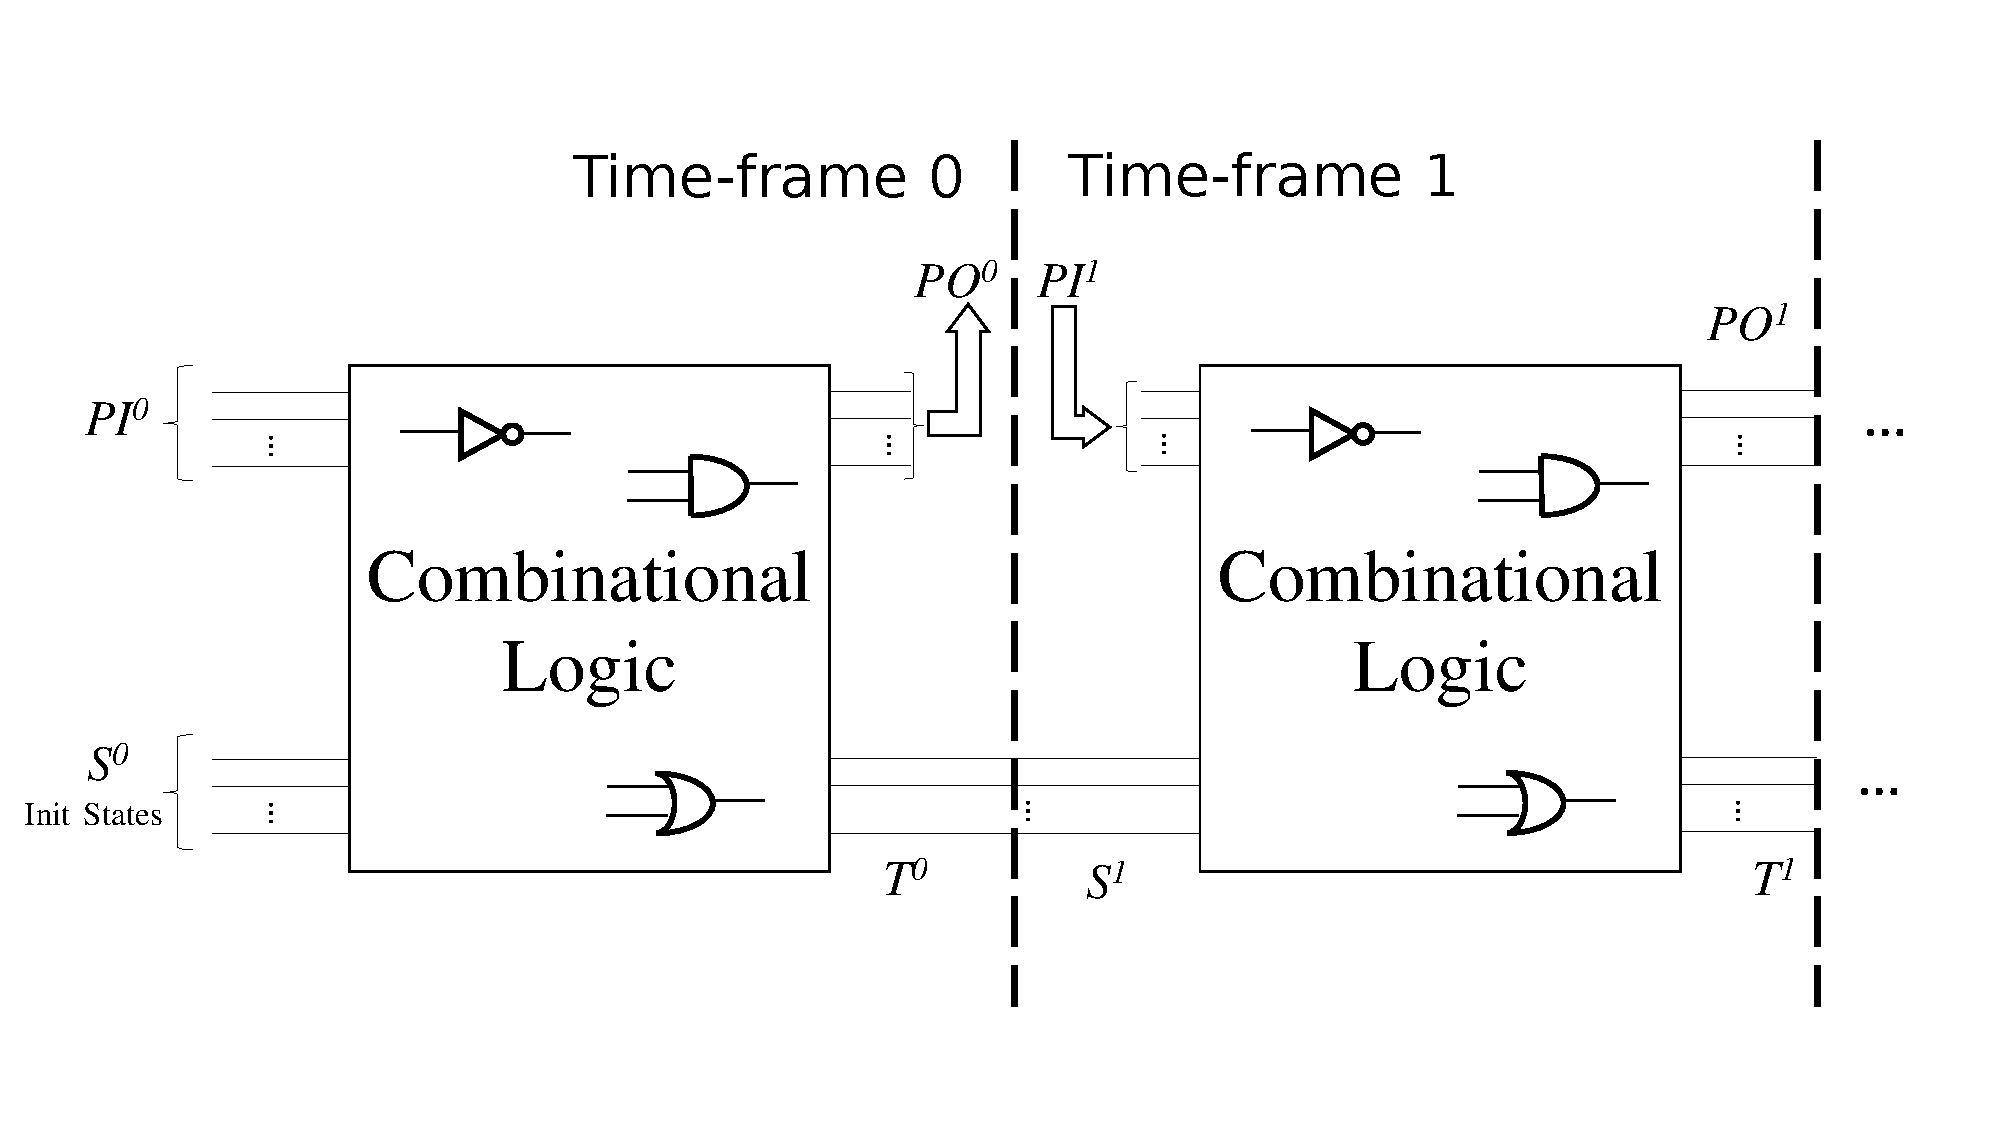
\includegraphics[width=\textwidth]{newfig/unroll.pdf}
}
\caption{The unrolling of a sequential circuit.}
\label{fig:unrolling}
\end{figure}

Unrolling provides a way to transform a sequential circuit into a combinational 
circuit. Therefore,  methods which can be applied to combinational circuit 
verification are also suitable for unrolled sequential circuits. The canonical 
graphical representation of the combinational circuit after unrolling is also 
the canonical representation of the original sequential circuit. For the sequential 
equivalence checking problem, we can also unroll the circuit to be verified and the 
specification to combinational ones, and then perform combinational equivalence checking
techniques \cite{savoj2010combinational}. In the following part we review research and techniques which 
can be applied to unrolled sequential circuits.

\subsection{Canonical Decision Diagrams}
The decision diagrams (DDs) are optimized data structures which can significantly accelerate formal verification.
The most fundamental DD is the Binary DD (BDD), which originates from the 
Shannon's expansion:
\begin{equation}
f(x, y, \dots) = x f_x + x' f_{x'}
\end{equation}
where $f_x = f(x = 1)$ and $f_{x'} = f(x = 0)$ denote the positive and
negative co-factors of $f$ {\it w.r.t.} $x$, respectively.
A BDD is usually represented as a binary tree.
Its ordered and reduced form, the Reduced Ordered Binary Decision Diagram (ROBBD)
\cite{BRYA86}, was the first significant contribution because of its canonicity.  
ROBDDs represent a Boolean function as an
implicit set of points on a canonical directed acyclic graph
(DAG). Manipulation of Boolean functions can then be carried out as
composition operations on their respective DAGs. An example of ROBDD is shown as Figure \ref{fig:BDD}.

Following BDDs,  variants of Shannon's decomposition principle
were explored to develop other functional decision diagrams such as
 FDDs \cite{okfdd}, ADDs \cite{add}, MTBDDs \cite{mtbdd}, and their hybrid 
edge-valued counterparts, HDDs \cite{hdd} and EVBDDs \cite{evbdd}. 
Zero-suppressed BDDs (ZDDs) \cite{minato1993zero,minato1994calculation} use the if-then-else branches
to represent the existence of variables in a cube, and result in lower 
space complexity. They can be used to represent polynomials with integer coefficients.

\begin{figure}[bp]
\centerline{
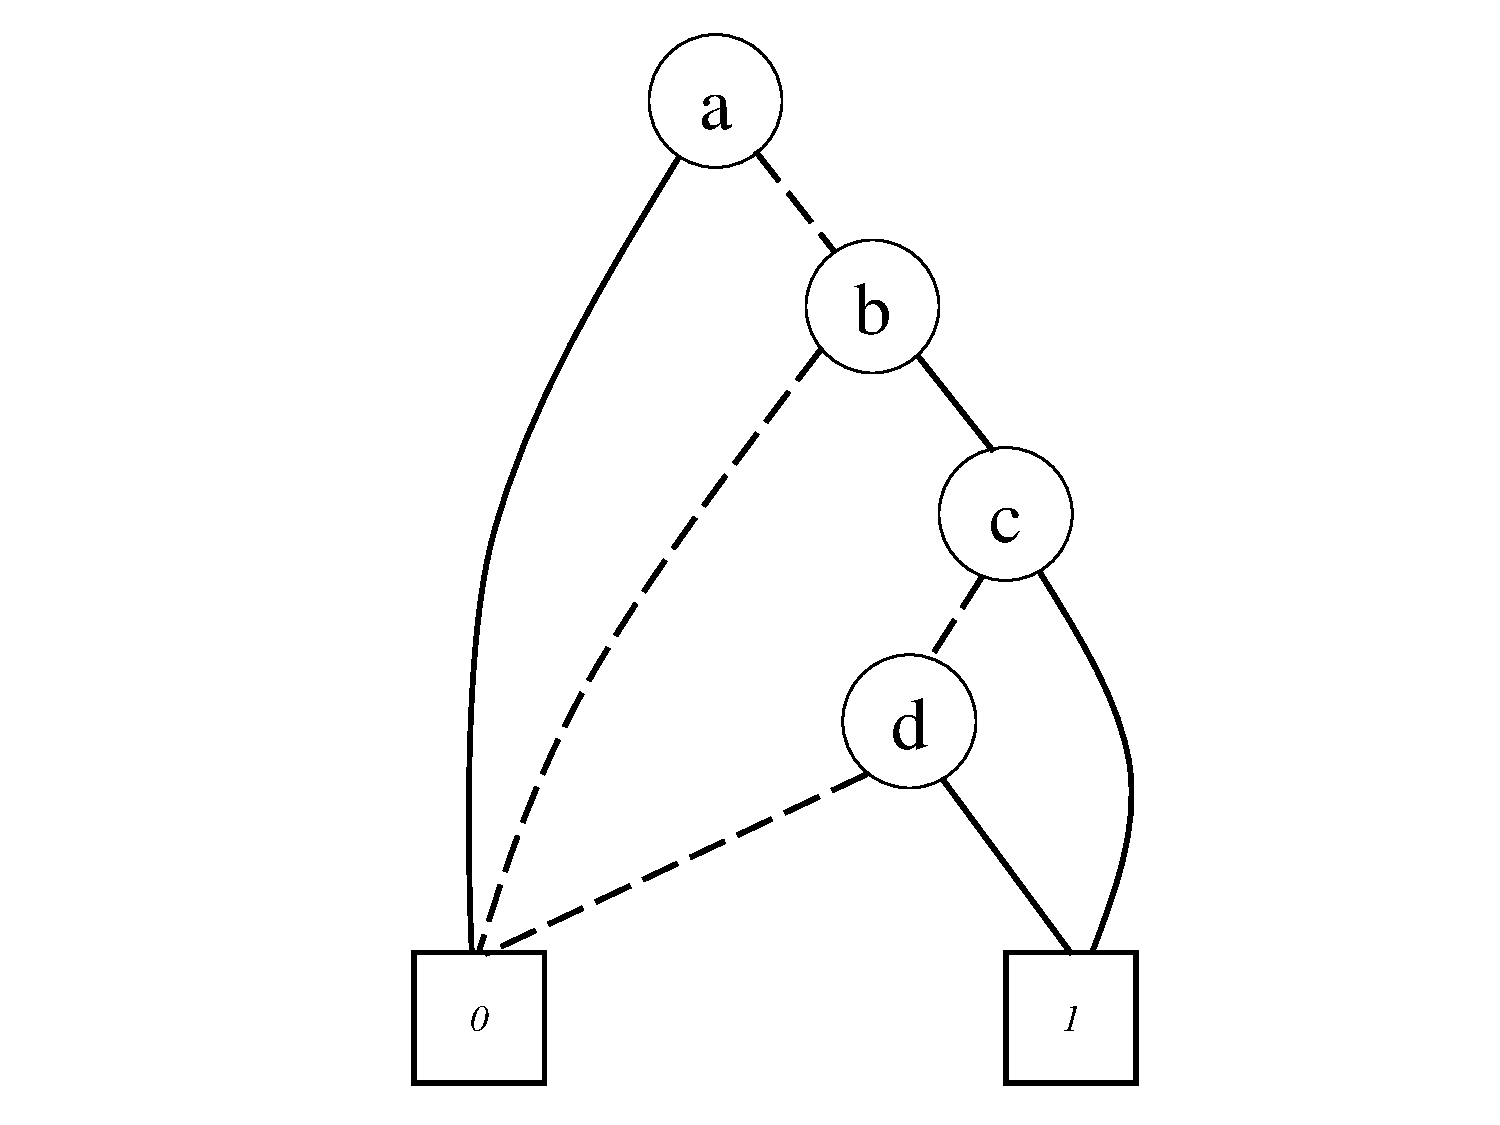
\includegraphics[width=0.45\textwidth]{newfig/BDD.pdf}
}
\caption{ROBDD representing Boolean function $\neg a \land b \land (c\lor d)$ with order $a>b>c>d$.}
\label{fig:BDD}
\end{figure}

The DDs above are all based on bit-level operations. Even in the {\it Word-Level Decision Diagrams}
\cite{WLS}, the decomposition is still point-wise, binary, 
w.r.t. each Boolean variable. These representations do not
serve the purpose of word-level abstraction from bit-level
representations. 

Binary Moment Diagrams (BMDs) \cite{bmd}, and their derivatives K*BMDs
\cite{kbmd} and *PHDDs \cite{phdd}, perform the decomposition of a {\it linear} function
based on its two moments instead of relying on Boolean decomposition. 
MODDs \cite{modd,modd_tcomp} are a DAG representation of the
characteristic function of a circuit over Galois fields $\Fkk$. 
However, MODDs fails to compactly represent large circuits.


Taylor Expansion Diagrams (TEDs) \cite{ted_tcomp} are a
word-level canonical representation of a {\it polynomial expression},
based on the Taylor's series expansion of a polynomial. However, they do
not represent a {\it polynomial function} canonically. 

The use of DDs in traditional formal verification has a lot of advantages. 
For example, DD-based model checking is very efficient as long as the DDs of sequential 
circuit can be setup. The existence of violating states in constructed DDs 
immediately deduces the violation of property. However, when the design gets
larger and larger, the time and space cost of building and storing the diagram 
increases rapidly. In our experiment of verifying a $k$-bit arithmetic circuit 
using ZDDs, when $k$ is larger than 100, the construction of ZDDs occupies 
over $99\%$ runtime of the whole procedure.
\subsection{Combinational Equivalence Checking Techniques}
The CEC problem can be solved using various methods.
Besides using canonical DDs (BDDs
\cite{BRYA86} and their word-level variants \cite{WLS}),
noncanonical representations such as And-Invert-Graph-based (AIG-based) reductions 
\cite{AIG:2002,alanmi:cec:iccad2006} are also very effective. 
Solvers for satisfiability problems (SAT) are good candidates to solve CEC problems,
as long as the miter of two circuits can be described using conjunctive normal form (CNF)
formulas. Applications of SAT on CEC include circuit-SAT solvers \cite{csat}, etc.
If the circuits being compared are structurally highly similar, AIG and circuit-SAT-based
approaches are known to be efficient.
However, when the circuits are functionally equivalent but structurally very dissimilar, none of the 
  contemporary techniques, including quantifier-free bit-vector 
  (QF-BV) theory-based SMT-solvers \cite{Cryptol:fmcad09},
  offer a practical solution.    


Recently integer polynomial based techniques \cite{ciesielski2014function,rolf:date16} have been proposed  to verify the functional 
correctness of integer arithmetic circuits. Their approach formulates the output signature as a polynomial function 
with binary variables and integer coefficients, then rewrites the polynomial by substituting gate output with gate 
inputs. After going through the backward rewriting procedure,  the polynomial
will be composed by only input variables. Then the polynomial is converted to a canonical representation, and compared
with a designated input signature. If they are equivalent, then the arithmetic circuit is successfully verified.
This approach incurs polynomial term explosion during the backward rewriting. The authors proposed a heuristic
to levelize the arithmetic circuit, and substitute several gates' variables at the same time to minimize the risk. However, 
the heuristic proved to be less effective when the inner symmetry of the circuit structure is missing.

% To conclude, automatic formal verification of large {\it
%     custom-designed modulo-arithmetic circuits} largely remains
%   unsolved today.
  
\section{Symbolic Model Checking and Abstraction Refinement}
Model checking is a way to verify certain safety and liveness properties 
in sequential circuits. Symbolic model checking, which avoids using explicit state encoding,
provides more flexibility to reduce the state space and enhance the 
efficiency of model checkers. The implementations of symbolic model checking 
require canonical DDs or SAT solvers \cite{burch1990sequential,burch1991representing,biere1999symbolic}.

Abstraction is a technique to reduce the state space representation by combining states with similar 
characteristics. Sometimes it can effectively lower the number of states that require analysis by orders of magnitude,
without affecting the properties we need to verify. Model checkers then utilize abstracted models 
with interpolation \cite{mcmillan2003interpolation,mcmillan:cav06}.
At first, abstraction was done manually by designers. Clarke {\it et al.} \cite{clarke2000counterexample}
proposed a BDD-based automated abstraction by removing spurious paths from analysis of counterexamples. 
Zhang {\it et al.} \cite{zhang2005design} proposed another abstraction method based on CNF-SAT.
It implemented latch abstraction by removing "irrelevant" latches by analyzing the 
UNSAT core from the $k$-BMC. Jain {\it et al.} \cite{jain2005word} improved the abstraction refinement technique of \cite{clarke2000counterexample},
where they use CNF-SAT to perform the refinement instead of using BDDs. The new approach is applied to verify RTL Verilog
and was known to be successful.

The $k$-BMC with interpolation is a purely incremental model-checking approach, and the interpolation procedure relies
on UNSAT core analysis. To overcome these weaknesses, a hybrid model checker called IC3 is developed 
\cite{bradley2011sat,bradley2011incremental}. IC3 works incrementally to find inductive subclauses
of negations of reached states, meanwhile it is monolithic when computing overapproximations to sets of reachable
states within $1,2,\dots,k$ steps. It is proved to be more efficient than interpolation-based model checking,
although using similar mechanisms.

The above techniques have limitations: they all rely on bit-level information from 
the circuit, which prevents them from being applied to circuits with large datapaths.
Meanwhile, their implementation relies on SAT/BDDs, which is an extension of Boolean 
functions and not compatible with other forms of constraints.

\section{Word-level Techniques Applied to Sequential Circuit Synthesis and Validation}
To better verify word-level designs, word-level verification techniques have been 
explored in recent years. Directly translating bit-vector problems to bit-level 
problems is called {\it bit-blasting}, and usually brings high redundancy and computational complexity in verification.
Attempts to develop pure word-level techniques can be found in
the rich domain of 
theorem proving \cite{arditi:bmd} and bit-vector SMT-solvers
\cite{boolector,cvc3,z3,bitvector98}, automated
decision procedures for Presburger arithmetic \cite{presburger,bultan:mixed_verification}, 
algebraic manipulation techniques 
\cite{devadas:algebraic_manipulation_iccd91}, or the ones based on
term rewriting \cite{AST}, etc.

Polynomial, integer, and other nonlinear representations have also
been researched: Difference Decision Diagrams (DDDs) \cite{ddd-csl99,ddd-mt-98}, interval
diagrams \cite{interval_dd}, interval analysis using polynomials
\cite{polynomial_sanchez99}, {\it etc.} Most of these have found 
application in constraint satisfaction for simulation-based
validation:  \cite{Ritter99,hsat,lpsat,brinkmann:asp-dac,Huang:tcad01,bitvector98}. Among
these, \cite{brinkmann:asp-dac,Huang:tcad01,bitvector98}
have been used to {\it solve} integer modular arithmetic on linear
expressions -- a different application from {\it representing}
finite field modulo-arithmetic on polynomials in a canonical form.   

Uninterpreted function abstraction is also an important category of 
word-level techniques which facilitates word-level model checking.
Usually uninterpreted symbols have no notion of bit-vector-precision. However, these techniques
constrain them 
using functional consistency among the evaluations of word variables
\cite{UF1,UF2,UF3}.


\section{Verification Using Algebraic Geometry}

Symbolic computer algebra techniques have been employed for formal
verification of circuits over $\Z_{2^k}$ and also over
Galois fields $\Fkk$. 
Verification techniques using Gr\"obner bases
\cite{Avrunin:CAV,gbverify:2007,manna:program} are proposed,
but they do not address the problem of high computational complexity to
compute Gr\"obner bases.

Verification of a combinational Galois field arithmetic circuit $C$ against a
polynomial specification $\Func$ has been previously addressed 
\cite{ibm:blueveri,lv:tcad2013,pruss:dac14}. Verification problems in
\cite{ibm:blueveri,lv:tcad2013} are formulated using
Nullstellensatz and decided using the \Grobner basis algorithm.

The paper 
\cite{pruss:dac14} performs verification by deriving a canonical
word-level polynomial representation $\Func$ from the circuit $C$. Their
approach views any arbitrary Boolean function (circuit) $f: \B^k
\rightarrow \B^k$ as a polynomial function $f: \Fkk \rightarrow \Fkk$,
and derives a canonical polynomial representation $\Func$ over
$\Fkk$. They show that this can be achieved by computing a reduced 
\Grobner basis {\it w.r.t.} an {\it abstraction term order} derived from the
circuit. Subsequently, they propose a \underline{r}efinement of this
\underline{a}bstraction \underline{t}erm \underline{o}rder (called
RATO) that enables them to compute the \Grobner basis of a smaller subset
of polynomials. The authors show that their approach can prove the
correctness of up to 571-bit combinational GF multipliers. 

IBM proposed a method to apply algebraic geometry techniques 
to verifying error coding circuits \cite{BLUEVERI}.
Recent papers \cite{rolf:date16,rolf:FMCAD16} provide a way to utilize 
algebraic geometry and GB-based symbolic computing and perform 
equivalence checking on integer arithmetic circuits and floating-point 
arithmetic circuits, respectively.

The use of algebraic geometry
for sequential circuit verification and symbolic model checking has
been presented before. Avrunin presented the
concept of symbolic MC using algebraic geometry in
\cite{Avrunin:CAV}. Later, in \cite{vardi-iasted07}, Vardi presented
GB-algorithms for CTL, LTL, and 
bounded MC over Boolean rings. However, these approaches are a
straightforward transformation of the problem to {\it bit-level}
Boolean GB engines which are used in lieu of BDDs or SAT solvers. All
the concepts of word-level reachability, abstraction-refinement using
interpolation or UNSAT cores, etc., that we desire were not the focus of
\cite{Avrunin:CAV,vardi-iasted07}. 

\section{Concluding Remarks}
From the investigation of previous work, techniques are to be researched that 
can perform the FSM traversal at word level to verify a property excluding spurious 
faults. Meanwhile, many abstraction refinement techniques utilize information from UNSAT cores.
We propose to solve these problems in the context of word-level verification,
with data representation, abstraction, and algorithm execution all carried out 
at word level.

In this dissertation, we propose a purely word-level reachability analysis approach, which has never been done before.
We achieve this by modeling the transition relations, states and the traversal algorithm at word level.
We borrow inspirations from \cite{tim:phd,gao:qe-gf-gb} to perform state space abstraction.
Moreover, we demonstrate applications of our proposed approach to sequential arithmetic verification, which has 
not been done before, either.
Finally, we show algebraic geometry analogs of UNSAT cores of polynomial ideals, and describe algorithms
to extract and refine these cores.

%%\input{myformulae.tex}


\section{Preliminaries}

\subsection{FSM model for sequential circuits}
A finite state machine (FSM) is a mathematical model of computation for designing and analyzing sequential logic 
circuits. If a FSM's primary outputs depend on primary inputs and present state inputs, it is named as a \textit{Mealy machine};
the formal definition is as follows:
\begin{Definition}
A Mealy machine is an $n$-tuple $\mathcal M = (\Sigma,O,S,S^0,\Delta,\Lambda)$ where
\begin{itemize}
\item $\Sigma$ is the input label, $O$ is the output label;
\item $S$ is the set of states, $S^0\subseteq S$ is the set of initial states;
\item $\Delta:\ S\times\Sigma\to S$ is the next state transition function;
\item $\Lambda:\ S\times\Sigma\to O$ is the output function.
\end{itemize}
\end{Definition}
The other kind of FSM is \textit{Moore machine}, its difference from Mealy machine is that
its primary outputs only depend on the present states, i.e. the output function is defined as
$$\Lambda:\ S \to O$$
Typical sequential circuits can be depicted as Fig.\ref{fig:seqmodel}(a). Primary inputs
$x_1,\dots,x_m \in \Sigma$, and primary outputs $z_1,\dots,z_n\in O$. Signals $s_1,\dots,s_k$ 
are present state (PS) variables, $t_1,\dots,t_k$ are next state (NS) variables.
We can define 2 $k$-bit words denoting the PS/NS variables as there are $k$ flip-flops
in the datapath: $S = (s_1,\dots,s_k), ~T=(t_1,\dots,t_k)$. Transition function
at bit level are defined as $\Delta_i: t_i = \Delta_i(s_1,\dots,s_k,x_1,\dots,x_m)$.
\begin{figure}[hbt]
\centering{
%\begin{minipage}{12cm}
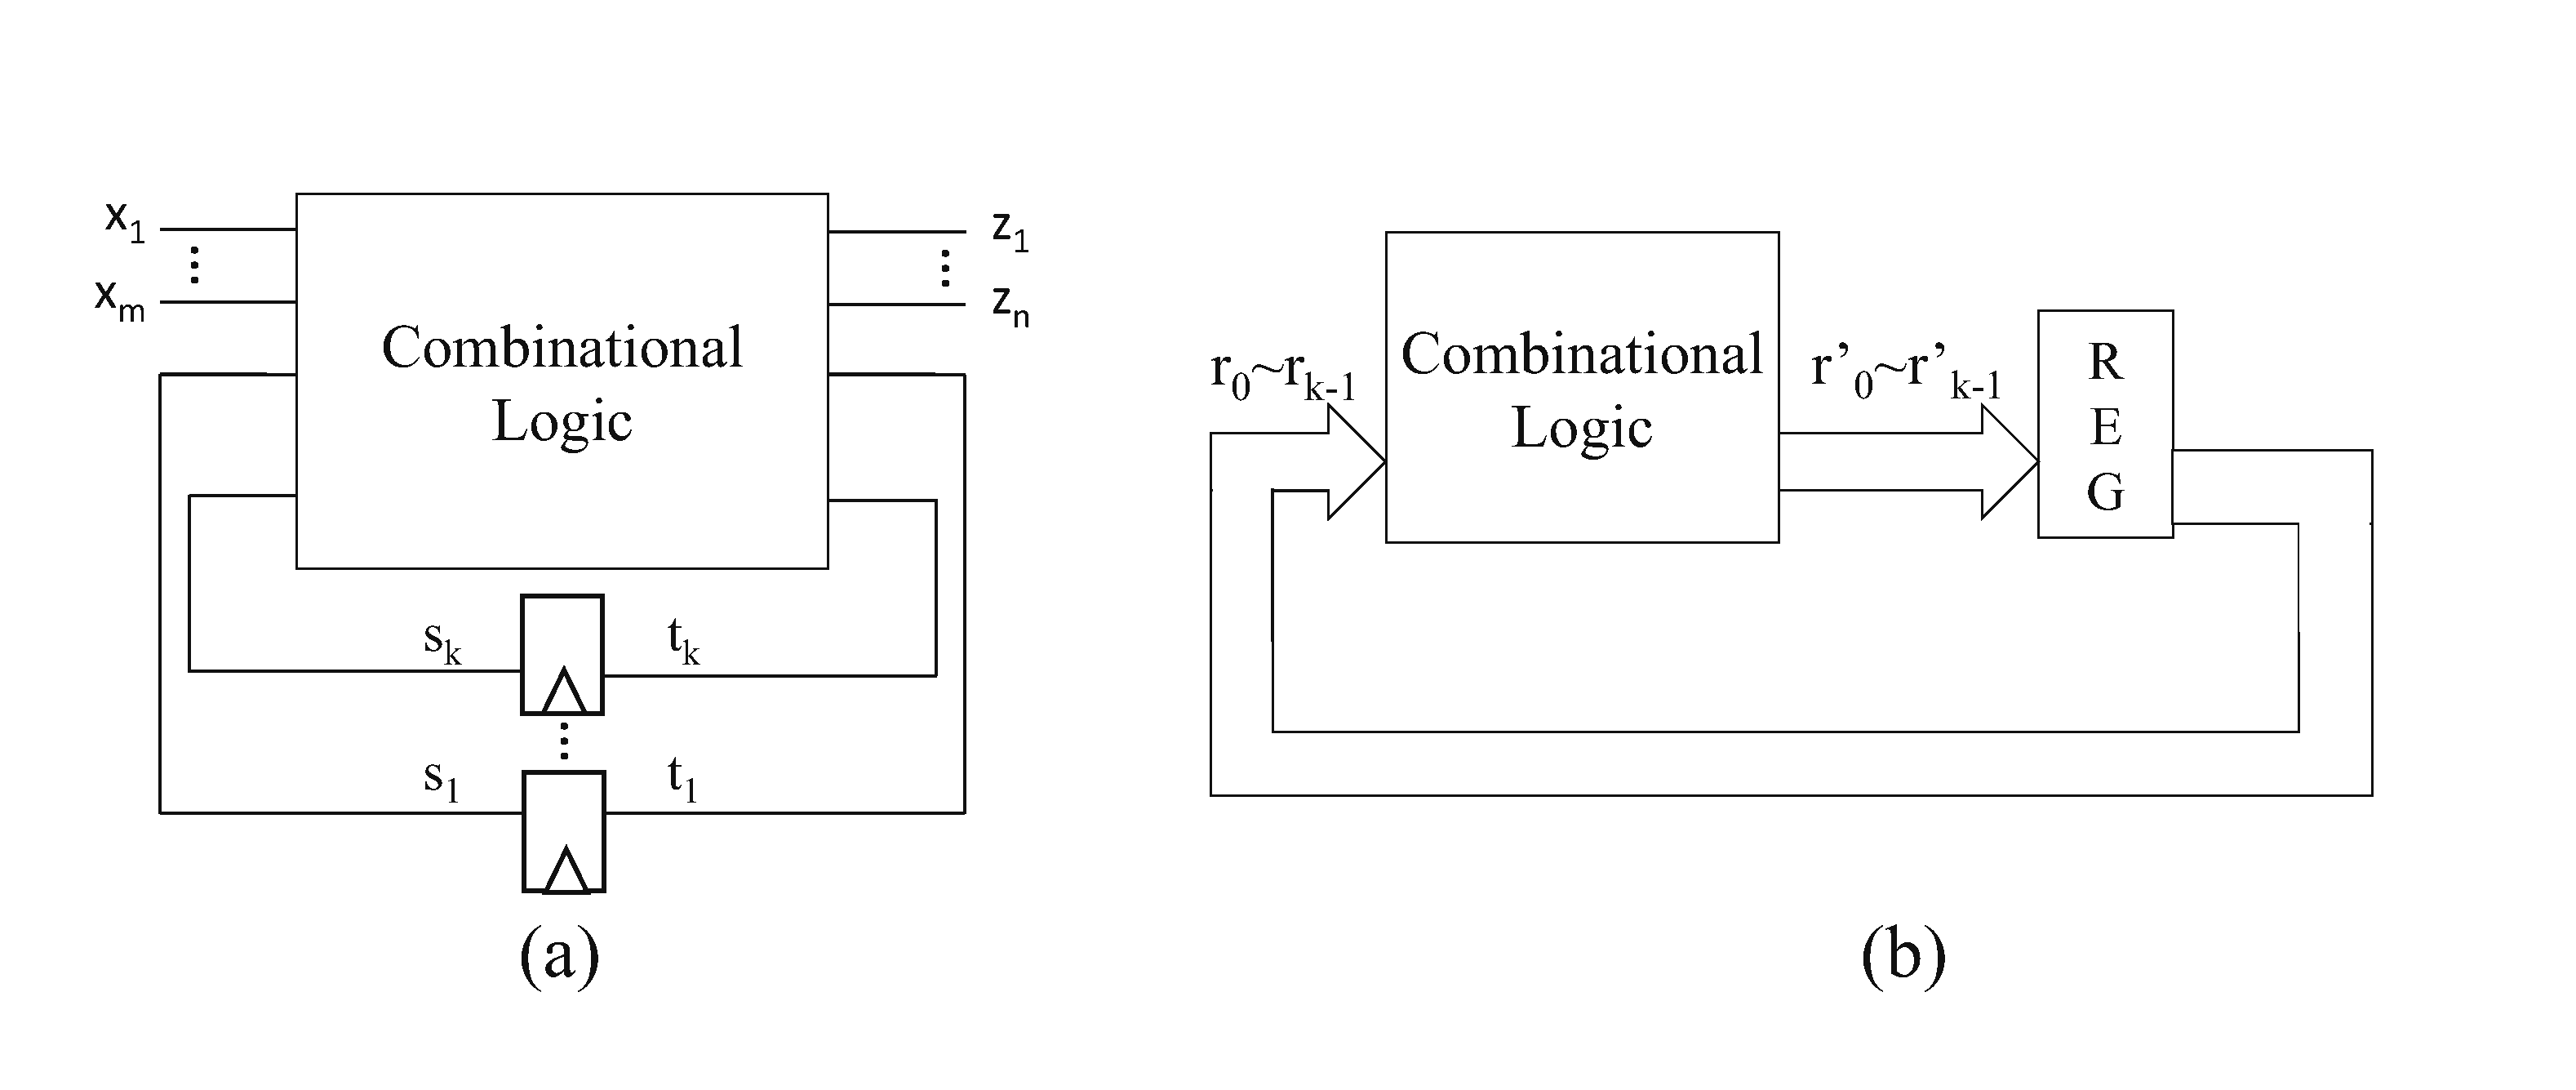
\includegraphics[width=3.5in]{./seqmodel.eps}
% \vspace{-0.2in}
\caption{FSM models of sequential circuits}
%\end{minipage}
\label{fig:seqmodel}}
\end{figure}
In some cases, arithmetic computations are implemented as Moore machines where input operands
are loaded into register files $R$ and the FSM is executed for $k$ clock cycles.
We can simplify them to the model in Fig.\ref{fig:seqmodel}(b).

\subsection{Commutative algebra and algebraic geometry preliminaries}
A {\bf field} $\mathbb{F}$ is a set of elements, including 0 and 1 (unity),
allowing for associative and commutative addition and multiplication;
and every non-zero element has a multiplicative inverse.  A {\bf
  finite field} or {\bf Galois filed} is a field with a finite number
($q$) of elements, and is denoted by $\Fq$, where $q=p^k$ is a power of
a prime integer $p$. In our work, $q = 2^k$ for
a given $k$, where $k$ represents the datapath (bit-vector)
word-lengths, or the number of memory elements (state registers) in
finite state machines. 

Let the field $\mathbb{F}_2 = \{0, 1\} ~(\equiv \B)$, and let
$\mathbb{F}_2[X]$ denote the set (ring) of all univariate polynomials
in variable $X$ with coefficients from $\mathbb{F}_2$. Then, the
Galois field $\Fkk$ is constructed as $\Fkk = \mathbb{F}_2[X] \pmod{
  P(X)}$, where $P(X)$ is an irreducible polynomial over
$\mathbb{F}_2$. Let $\alpha$ be a root of the irreducible polynomial
$P(X)$, i.e. $P(\alpha) = 0$. Any element $A \in \Fkk$ can be
represented as $A = \sum_{i=0}^{k-1} a_i \alpha^i$, where $a_i \in
\mathbb{F}_2$. The field $\Fkk$ is therefore, a $k$-dimensional {\it
  extension} of the base field $\mathbb{F}_2$: so,  $\mathbf{\Fkk \supset
\mathbb{F}_2}$. Consequently, all operations of addition and
multiplication in $\Fkk$ are performed modulo the irreducible
polynomial $P(\alpha)$ and coefficients are reduced modulo 2.  

Boolean variables in field $\mathbb B$ can be easily mapped to
elements in $\mathbb F_2$. Since $\mathbb F_2 \subset \Fkk$, these 
%Namely $k$-bit Boolean bit-vector defined
%over Boolean ring $\mathbb B^k$ can also be mapped uniquely  to $\Fkk
%= \mathbb F_2[x_1,\dots,x_k]$. 
Boolean operators are interpreted as functions over $\Fkk$ (where $+$
and $\cdot$ are addition and multiplication performed modulo 2): 
\begin{align*}
&a\land b \to a\cdot b\\
&a\oplus b \to a+b\\
&\neg a \to 1+a\\
&a \bar{\oplus} b \to 1+a+b\\
&a \lor b \to a+b+a\cdot b
\end{align*}

Using these mappings we can write Boolean functions in form of
polynomials over $\mathbb F_2\subset \Fkk$. 
These concepts provide a mechanism to represent and
manipulate both bit-level ($\mathbb{F}_2$) and $k$-bit word-level
constraints {\bf in one unified mathematical domain $\Fkk$ --- a
  concept we   exploit for abstraction. }
  Consider Ex.\ref{ex:motiv},
polynomials for transition functions (bit-level outputs) $f_1,f_2$
are over $\mathbb F_2$, i.e. $f_1,f_2\subseteq \mathbb F_2 \subset \Fkk$,
and polynomials containing word-level variables $f_3,f_4,f_5 \subseteq \Fkk$.
All polynomials belong to unified domain $f_1,f_2,\dots,f_5 \subseteq \Fkk$.

It is well-known that every Boolean mapping between $k$ dimensional
Boolean spaces $f: \B^k \rightarrow \B^k$ can be construed as a
function over Galois fields $f: \Fkk \rightarrow \Fkk$. Moreover,
every function $f: \Fkk \rightarrow \Fkk$ is a polynomial function: 
i.e. $f$ can be represented by way of a unique, minimal, canonical
polynomial $\F(X)$, and the work of \cite{timDAC} shows how to
efficiently derive such polynomial representations from circuits ---
another concept that makes our approach feasible. 


We represent Boolean circuits by way of polynomials over
$\Fkk$. If we take indeterminates $x_1,x_2,\dots,x_n$, an arbitrary
combination of their finite product  
$x_1^{d_1}\cdot x_2^{d_2}\cdots x_n^{d_n}, d_i\geq 0$ 
is a {\bf monomial}. A {\bf polynomial} $f = c_1 X_1 + c_2 X_2 + \dots
+ c_t X_t$ is a finite sum of terms, where $c_1, \dots, c_t$ are
coefficients and $X_1, \dots, X_t$ are monomials. The set of {\it all}
such polynomials with coefficients from $\Fkk$ forms a {\bf
  multivariate polynomial ring} denoted $\Fkk[x_1,\dots,x_n]$. 
A monomial ordering $X_1 > X_2 \dots > X_t$ is imposed on the
polynomials to process them systematically. Then, $LT(f) = c_1 X_1,
LM(f) = X_1$ denote the leading term and the leading monomial of $f$,
respectively. 


Multivariate polynomial division will play a key role in our
algorithmic techniques. Division is implemented as {\it cancellation
  of terms.} Given polynomials $f, g$, if $cX$ is a term in
$f$ that is divisible by $LT(g)$, then $f \xrightarrow{g} r$ denotes a
one-step reduction (division) of $f$ by $g$, resulting in remainder $r
= f - {{cX} \over {LT(g)}} \cdot g$. This has the effect of cancelling
the term $cX$ from $f$. 
\begin{Example}
\label{ex:multidiv}
If $f = e + cd$ and $g = c + ab$,
then the term $cd$ in $f$ can be canceled by $LT(g) = c$: $r = f - {cd
  \over c} g = e + abd$. 
\end{Example}
  Similarly, $f$ reduces to $r$ modulo the set
of polynomials $F = \{f_1, \dots, f_s\}$, denoted $f \stackrel{F}
{\textstyle   \longrightarrow}_+ r$, such that no term in $r$ is
divisible (cancellable) by the $LT(f_i)$ of any polynomial in $ f_i
\in F$.    


In verification, we have to analyze the {\it solutions to a
set of polynomials.} The set of all solutions to a system of
polynomial equations $f_1 = \dots = f_s = 0$ is defined as the affine variety:
\begin{Definition}
Given a set of polynomials $f_1,\dots,f_s$ over ring $\mathbb F_q[x_1,\dots,x_n]$, their 
{\bf affine variety} 
$$V(f_1,\dots,f_s) = \{(a_1,\dots,a_n)\in  (\mathbb F_q)^n |
f_1(a_1,\dots,a_n) = \cdots = f_s(a_1,\dots,a_n) = 0\}$$ 
\end{Definition}

Generally we can find many sets of polynomials with the same variety, which are linear combinations
of given set of polynomials. This set is defined as follows:
\begin{Definition}
{\bf Ideal of Polynomials:} Let $f_1,f_2,\dots,f_s\in \mathbb F[x_1,\dots,x_n]$.
Define an ideal
$$J = \langle f_1,f_2,\dots,f_s\rangle = \{f_1\cdot h_1 + f_2\cdot h_2 +\cdots + f_s\cdot h_s : h_1,\dots,h_s\in \mathbb F[x_1,\dots,x_n]\}$$
We call $J = \langle f_1,f_2,\dots,f_s\rangle$ an ideal generated by $f_1,\dots,f_s$ and these polynomials 
the {\bf generators} of ideal $J$.
\end{Definition}
% On the other hand, if given another polynomial $f$, we need to judge whether it belongs to $J$.
A practical problem is: given an ideal $J = \langle f_1,f_2,\dots,f_s\rangle$ and a polynomial $f$,
we need to check if the variety of $J$ can make the evaluation of $f$ equal to 0, i.e. $f$ vanishes on $V(J)$.
This problem is usually described as ideal membership checking problem.
\begin{Definition}
{\bf Ideal membership:} Let $f_1,f_2,\dots,f_s\in \mathbb F[x_1,\dots,x_n]$, and $J = \langle f_1,f_2,\dots,f_s\rangle$
be an ideal over ring $\mathbb F[x_1,\dots,x_n]$. If 
$$f = f_1h_1 + f_2h_2 + \cdots + f_sh_s$$
then $f\in J$.
\end{Definition}

An ideal may have many generating sets. For example, we may have different set of polynomial generators denoting
the same ideal, where they have the same variety: $\langle f_1,\dots,f_s\rangle = \langle h_1,\dots,h_r\rangle
= \langle g_1,\dots,g_t\rangle$ such that $V(f_1,\dots,f_s) = V(h_1,\dots,h_r) = V(g_1,\dots,g_t)$.
Therefore a canonical representation of an ideal is needed, which leads to the concept of Gr\"obner bases.

\begin{Definition}
The set $G = \{g_1, \dots,
g_t\}$ is called a \textbf{\Grobner basis} of $J$ if and only if the
leading term of all polynomials in $J$ is divisible be the leading
term of some polynomial $g_i$ in $G$: i.e. $\forall f \in J, \exists
g_i \in G \ s.t. \ LT(g_i) ~|~ LT(f)$. 
\end{Definition}
% The famous Buchberger's
% algorithm, given in textbook \cite{ideals:book}, is used to compute a
% \Grobner basis (GB). Operating on  input $F = \{f_1, \dots, f_s\}$,
% and subject to the imposed term order $>$, it derives $G = GB(J) = \{
% g_1, \dots, g_t \}$. Buchberger's algorithm repeatedly computes
% $S$-polynomials. For pairs $(f_i, f_j) \in F$, $Spoly(f_i, f_j) =
% \frac{L}{lt(f_i)}\cdot f_i - \frac{L}{lt(f_j)}\cdot f_j$, where $L =
% LCM(LM(f_i), LM(f_j))$. Reducing $Spoly(f_i, f_j) \xrightarrow{F}_+ r$
% cancels the leading terms of $f_i, f_j$ and gives a polynomial $r$
% with a new leading term. This remainder $r$ is added to the current
% basis and $Spoly(f_i, f_j)$ computations are repeated for all pairs of
% polynomials until all $S$-polynomials reduce to 0.  

An advantage of representing an ideal with GB is that it can serve as a decision procedure for ideal membership
test when dividing a polynomial $f$ by a GB, i.e.
$$G = GB(J) \Longleftrightarrow \forall f\in J, f\xrightarrow{g_1,g_2,\dots,g_t}_{+} 0$$
Gr\"obner basis can be reduced by eliminating redundant elements. \textbf{A reduced GB is a canonical representation of 
the ideal under a given monomial ordering}. Given an ideal $J = \langle f_1,\dots,f_s\rangle, ~G = 
\{g_1,\dots,g_t\}$ is the GB of $J$, it can be computed by Buchberger's algorithm (refer to textbook \cite{ideal:book}).

Another advantage of using GB representation is that GB computation can work as a {\it quantification procedure}.
In the following part we will introduce the concept of \textit{vanishing polynomials}, \textit{elimination ideal}, etc.
as the bases of this theory.

{\it Fermat's little theorem over $\Fq$:} For any $ \alpha \in \mathbb
F_{q}, \alpha^q = \alpha$. Therefore, the polynomial $x^q - x$
vanishes ($=0$) over $\Fq$, and is called a vanishing polynomial. We
denote by $J_0 = \langle x_1^q - x_1, \dots, x_d^q - x_d \rangle$ the
ideal of all vanishing polynomials in $\Fq[x_1, \dots, x_d]$. When $q
= 2^k, x^q - x = x^q + x$ as $-1 = +1$ over $\Fkk$.

Gr\"obner bases can be used to {\it eliminate} (i.e. quantify) variables from an
ideal. Given ideal $J = \langle f_1,\dots,f_s\rangle \subset \mathbb
F_{q}[x_1,\dots,x_d]$, the $l^{th}$ elimination ideal $J_l$ is the
ideal of $\Fq[x_{l+1}, \dots, x_d]$ defined by $J_l = J \cap
\Fq[x_{l+1}, \dots, x_d]$. Variable elimination can be achieved 
by computing a Gr\"obner basis of $J$ w.r.t. elimination orders: 
\begin{Theorem}
\label{thm:elim}
(Elimination theorem\cite{ideals:book}) Let $J\subset \mathbb
  F_{2^k}[x_1,\dots,x_d]$ be an ideal and let $G$ be a Gr\"obner basis
  of $J$ with respect to a lexicographic (LEX) ordering where
  $x_1>x_2>\cdots>x_d$. Then for every $0\leq l\leq d$, the set $G_l =
  G\cap\mathbb F_{2^k}[x_{l+1},\dots,x_d]$ is a Gr\"obner basis of
  the $l$-th elimination ideal $J_l$.
\end{Theorem}
We describe an application of elimination ideals using following example borrowed from \cite{ideals:book}:
\begin{Example}
Consider polynomials $f_1: x^2-y-z-1;\ f_2:x-y^2-z-1;\ f_3:x-y-z^2-1$ and ideal $J = \langle f_1,f_2,f_3\rangle
\subset \mathbb C[x,y,z]$. Gr\"obner basis $G = GB(J)$ w.r.t. LEX term order equals to 
$g_1:x-y-z^2-1;\ g_2:y^2-y-z^2-z;\ g_3: 2yz^2-z^4-z^2;\ g_4:z^6-4z^4-4z^3-z^2$. From observation,
we find that the polynomial $g_4$ only contains variable $z$ ($x,y$ eliminated), and polynomials $g_2,g_3,g_4$ only contain variables
$y,z$ ($x$ eliminated). According to theorem \ref{thm:elim}, $G_1 = G\cap\mathbb C[y,z] = \{g_2,g_3,g_4\}$
is the Gr\"obner basis of the $1^{st}$ elimination ideal of $J$ and $G_2 = G\cap\mathbb C[z] = \{g_4\}$ is the 
$2^{nd}$ elimination ideal of $J$, respectively.
\end{Example}

\subsection{Application of elimination theorem on circuit verification}
\label{sec:elim}
Assume that we are given a circuit (combinational component) with input $A = (a_0,\dots,a_{k-1})$ and output 
$R = (r_0,\dots,r_{k-1})$ (both can be represented
by word level variables in $\Fkk$). We can describe this circuit with an elimination ideal $J+J_0$, where
$J$ is the ideal generated by the polynomials corresponding to circuit gates and $J_0$ is the ideal of vanishing polynomials.
The authors of \cite{timDAC} showed that for any combinational
logic block, a canonical word-level polynomial representation can be
derived through \Grobner bases computed with elimination orders:
\begin{Lemma}
(From \cite{timDAC}) Given a combinational circuit $C$ with $k$-bit
  input $A = (a_0, \dots, a_{k-1})$ and $k$-bit output $R = (r_0, \dots,
  r_{k-1})$. Denote by $x_1, \dots, x_d$ all the bit-level
  variables of   $C$. Let $J = \langle f_1, \dots, f_s \rangle \subset
  \Fkk[x_1, \dots, x_d, R, A]$ denote all the polynomials corresponding to the
  logic gates of the circuit. Let $J_0 = \langle x_1^2 - x_1, \dots,
  x_d^2 - x_d, R^q - R, A^q - A \rangle$ be the vanishing ideal, so
  that $J + J_0 = \langle f_1, \dots, f_s, ~~ x_1^2 - x_1, \dots,
  x_d^2 - x_d, R^q - R, A^q - A \rangle$. Compute \Grobner basis $G =
  GB(J + J_0)$ w.r.t. lex term order with $x_1 > x_2 > \dots > x_d > R
  > A$. Then $G_d = G \cap \Fkk[R, A]$ eliminates the internal
  variables $x_1, \dots, x_d$ of the circuit. $G_d$ also contains the
  word-level polynomial $R = \F(A)$ which canonically represents the
  function of the circuit with only word level variables $R$ and $A$.
\end{Lemma}
This lemma shows an application of GB computations over an elimination ideal.
Since it abstracts the function of a combinational circuit, we call the term order
$primary~inputs~and~intermediate~variables~>~word~level~output~>~word~level~inputs$
as \textit{abstraction term order} (ATO).
If we further eliminate word-level input, the result will be a polynomial containing only 
the word-level output variable. In a sequential circuit
such as Ex.\ref{ex:motiv}, the output of combinational logic serves as the next state variable. Polynomial $g_T$ in
the example is the desired projection; i.e. using GB computation on elimination ideal and eliminating to NS
variables provides us the canonical representation of reachable states in next time frame.



% Machine traversal is key for many verification techniques, e.g. to check
% the equivalence of 2 FSMs, we can observe whether the output responses are the same at
% every step of traversal. An explicit traversal is usually infeasible, here we use 
% implicit state enumeration (BFS traversal) based on Boolean formulas to implement a machine traversal.
% The algorithm is as follows:
% \begin{algorithm}[hbt]
% \SetAlgoNoLine
%  \KwIn{Transition functions $\Delta$, initial state $S^0$}
% 
%   $from^0 = reached = S^0$\;
%   \Repeat{$new^i == 0$}
%   {
%   	$i \gets i + 1$\;
% 	$to^i \gets$Img$(\Delta, from^{i-1})$\;
% 	$new^i \gets to^i \cap \overline{reached}$\;
%   	$reached \gets reached \cup new^i$\;
% 	$from^i \gets new^i$\;
%   }
% \Return{$reached$}
% \caption {Breadth-first Traversal Algorithm for Reachability Analysis of FSMs}\label{alg:BFS}
% \end{algorithm}
% The main computation in this algorithm is the \textit{image function}. Img$(\Delta,from^{i-1})$
% denotes the forward image of the set $from^{i-1}$ under the transition function $\Delta$.
% Let  $\Delta_i$ denote the transition relation 
% for $i^{th}$ bit of output $T$ (denoted by $t_i$), and it is described by a Boolean function. We can obtain the transition relation 
% for bit-vector $T$: $Tran(s_0,s_1,x,t_0,t_1) = \bigwedge_{i=1}^{2}(t_i\ \bar{\oplus}\ \Delta_i)$. Assume present states
% are represent by Boolean formulas $PS(s_0,s_1)$, then the image function is written as
% $\text{Img}(Tran,\ PS) = \exists_{s_0,s_1}\exists_{x}[Tran(s_0,s_1,x,t_0,t_1)\land PS(s_0,s_1)]$, where
% $\exists_x f$ denotes the existential quantification of $f$ w.r.t. $x$.
% \begin{Example}
% We use implicit state enumeration based on Boolean formulas to traverse FSM in Fig.\ref{fig:fsm}.
% Initial state $\{00\}$ can be represented by Boolean formula $C(s) = \overline{s_0}\cdot \overline{s_1}$.
% Transition function for $NS$ variables are 
% $$t_0\overline{\oplus}\Delta_0 = t_0\overline{\oplus}(\overline{x}\overline{s_0}\overline{s_1}+s_0s_1)$$
% $$t_1\overline{\oplus}\Delta_1 = t_1\overline{\oplus}(x\overline{s_0}+s_0\overline{s_1})$$
% \end{Example}
\chapter{Finite Fields and Sequential Arithmetic Circuits}
\label{ch:prelim_GF}
This chapter provides a mathematical background for understanding 
finite fields (Galois fields) and explains how to design Galois field (GF) arithmetic circuits.
We first introduce the mathematical concepts of groups, rings, fields, and 
polynomials. 
We then apply these concepts to create Galois field arithmetic functions and 
explain how to map them to a Boolean circuit implementation.
Additionally, we introduce a special type of sequential arithmetic hardware based on normal basis, as well
as the normal basis theory behind the designing such hardware.

The material is referred from \cite{galois_field:mceliece, ftheory:2006, ff:1997} for Galois field concepts, 
\cite{mastro:1989, PT:1985, acar:1998, wu:2002, Knezevic:2008} for hardware design over Galois fields 
and previous work by Lv \cite{lv:phd}.
Normal basis theory in this section is referred from \cite{normal_book, gao:phd_normal_basis} and sequential
normal basis arithmetic hardware designs come from \cite{mullinONB,MasseyOmura,agnew1991implementation, RHmulti}.

\section{Commutative Algebra}
\label{sec:algebra}
\subsection{Group, Ring and Field}
\begin{Definition}
An {\bf Abelian group} is a set $\mathbb{S}$ with a binary operation $'+'$
which satisfies the following properties: 
\begin{itemize}
\item {\it Closure Law:} For every $a, b \in \mathbb{S}, a + b \in \mathbb{S}$  
\item {\it Associative Law:} For every $a, b, c \in \mathbb{S}, (a + b) + c = a + (b + c)$
\item {\it Commutativity:} For every $a, b \in \mathbb{S}, a + b = b + a$. 
\item {\it Additive Identity:} There is an identity element $0 \in \mathbb{S}$
such that for all $a \in \mathbb{S};$ $a + 0 = a$.
\item {\it Additive Inverse:} If $a \in \mathbb{S}$, then there is an
element $a^{-1} \in \mathbb{S}$ such that $ a + a^{-1} = 0$.
\end{itemize}
\end{Definition}

The set of integers $\mathbb{Z}$ forms an Abelian group under the addition operation. 

\begin{Definition}
Given a set $\mathbb{R}$ with two binary operations, $'+'$ and $'\cdot'$, 
and element $0 \in \mathbb{R}$, the system $\mathbb{R}$ is called a {\bf commutative ring with unity} if the following properties hold:
\begin{itemize}
\item $\mathbb{R}$ forms an Abelian group under the '+' operation with additive identity element $0$.
\item {\it Multiplicative Distributive Law}: For all $a, b, c \in$ $\mathbb{R}$, $a\cdot (b + c) = a\cdot b + a\cdot c$.
\item {\it Multiplicative Associative Law}: For every $a, b, c\in \mathbb{R}$, $a\cdot (b\cdot c) = (a\cdot b)\cdot c$. 
\item {\it Multiplicative Commutative Law}: For every $a,b \in \mathbb{R}$, $a\cdot b = b\cdot a$
\item {\it Identity Element}: There exists an element $1 \in$ $\mathbb{R}$ 
such that for all $a \in \mathbb{R}$, $a\cdot 1 = a =1\cdot a$
\end{itemize}
\end{Definition}

{\bf Ring} is a broad algebraic concept. In this dissertation, this word is used to refer a special 
sort of ring -- {\bf commutative ring with unity}. Two common 
examples of such rings are the set of integers, $\mathbb{Z}$, and the set of 
rational numbers, $\mathbb{Q}$. While both of these examples are
rings with an infinite number of elements, the number of elements in a ring 
can also be finite, such as the ring of integers modulo $n$ ($\Z_n$).

\begin{Definition}
A {\bf field} $\mathbb{F}$ is a commutative ring with unity, where every
non-zero element in $\mathbb{F}$ has a multiplicative inverse; {\it i.e.} $\forall
a \in \mathbb{F} - \{0\}$, $\exists \hat{a} \in \mathbb{F}$ such that $ a \cdot
\hat{a} = 1$.
\end{Definition}

A field is defined as a ring with one extra condition: the presence of a 
multiplicative inverse for all non-zero elements.
Therefore, a field must be a ring while a ring is not necessarily a field.
For example, the set $\mathbb{Z}_{2^k} = \{0,1,\cdots, 2^k-1\}$ forms a finite ring.
However, $\mathbb{Z}_{2^k}$ is not a field because not every element in
$\mathbb{Z}_{2^k}$ has a multiplicative inverse. 
In the ring $\mathbb{Z}_{2^3}$, for 
instance, the element $5$ has an inverse ($5\cdot5\pmod{8}=1$) but the element $4$
does not.

An important concept in field theory is {\bf field extension}. The idea behind a
field extension is to take a base field and construct a larger field which 
contains the base field as well as satisfies additional properties. For example,
the set of real numbers $\mathbb{R}$ forms a field; one extension of 
$\mathbb{R}$ is the set of complex numbers $\mathbb{C}=\mathbb{R}(i)$. Every
element of $\mathbb{C}$ can be represented as $a+b\cdot i$ where $a,b \in \mathbb{R}$,
hence $\mathbb{C}$ is a two-dimensional extension of $\mathbb{R}$.

Like rings, fields can also contain either an infinite or a finite number of 
elements. 
In this dissertation we focus on finite fields -- also known as Galois fields, 
the construction of their field extensions, and their applications on circuit verification and abstraction techniques.

\subsection{Finite Field}
Finite fields find widespread applications in 
many areas of electrical engineering and computer science such as error-
correcting codes, elliptic curve cryptography, digital signal processing, 
testing of VLSI circuits, among others.
In this dissertation, we specifically focus on their application to 
the FSM traversal of sequential Galois field circuits as well as abstraction refinement based on UNSAT core extraction.
This section describes the relevant Galois field concepts
\cite{galois_field:mceliece} \cite{ftheory:2006} \cite{ff:1997}
and hardware arithmetic designs over such fields \cite{mastro:1989} \cite{PT:1985} 
\cite{acar:1998} \cite{wu:2002} \cite{Knezevic:2008}. 

%%%%%%%%%%%%%%%%%%%%%%%%%%%%%%%%%%%%%%%%%%%%%%%%%%%%%%%%%%%%%%%%%%%%%%%%%%%%

\begin{Definition} 
A {\bf Galois field}, denote $\Fq$, is a field with a finite
number of elements, $q$. The number of elements $q$ of the field is
a power of a prime integer, {\it i.e.} $q = p^k$, where $p$ is a prime
integer, and $k \geq 1$. Thus a Galois field can also be denoted as 
$\F_{p^{k}}$.
\end{Definition}

Fields of the form $\F_{p^{k}}$ are called Galois extension fields.
We are specifically interested in extension fields of type 
$\Fkk$, where $k > 1$. These are extensions of the binary
field $\F_2$.

\begin{table}[!h]
\caption{Addition and multiplication operations over $\F_2$.}
	\centering
	\begin{tabular}{m{1cm}|l|ll|m{1cm}}
	\hhline{~---~}
	\multirow{3}{*}{} & $+$ & $0$ & $1$ & \multirow{3}{*}{} \\
	\hhline{~---~}
	& $0$ & $0$ & $1$ & \\
	& $1$ & $1$ & $0$ & \\
	\hhline{~---~}
	\multicolumn{5}{c}{}\\
	\multicolumn{5}{c}{Addition over $\F_2$}\\
	\end{tabular}
	\quad
	\begin{tabular}{m{1cm}|l|ll|m{1cm}}
	\hhline{~---~}
	\multirow{3}{*}{} & $\cdot$ & $0$ & $1$ & \multirow{3}{*}{} \\
	\hhline{~---~}
	& $0$ & $0$ & $0$ & \\
	& $1$ & $0$ & $1$ & \\
	\hhline{~---~}
	\multicolumn{5}{c}{}\\
	\multicolumn{5}{c}{Multiplication over $\F_2$}\\
	\end{tabular}
\end{table}

Notice that addition over $\F_2$ is a Boolean {\sc XOR} operation, 
because it is performed modulo $2$.
Similarly, multiplication over $\F_2$ performs a Boolean {\sc AND} operation.


Algebraic extensions of the binary field $\F_{2}$  
are generally termed as {\it binary extension fields} $\Fkk$.
Where elements in $\F_2$ can only represent $1$ bit, elements in $\Fkk$ 
represent a $k$-bit vector.
This allows them to be widely used in digital hardware applications.
In order to construct a Galois field of the form $\Fkk$, 
an {\bf irreducible polynomial} is required:
\begin{Definition}
A polynomial $P(x) \in \mathbb{F}_{2}\left[x\right]$, {\it i.e.} the set of all 
polynomials in $x$ with coefficients in $\F_2$, is {\bf irreducible} 
if $P(x)$ is non-constant with degree $k$ and cannot be 
factored into a product of polynomials of lower degree in $\mathbb{F}_2[x]$.
\end{Definition}

Therefore, the polynomial $P(x)$ with degree $k$ is irreducible over 
$\mathbb{F}_{2}$ if and only if it has no roots in $\mathbb{F}_{2}$,
i.e if $\forall a \in \mathbb{F}_{2}$, $P(a)\neq 0$.
For example, $x^2+x+1$ is an irreducible polynomial over $\mathbb{F}_{2}$
because it has no solutions in $\mathbb{F}_{2}$, {\it i.e.} $(0)^2+(0)+1=1\neq0$ 
and $(1)^2+(1)+1=1\neq0$ over $\F_2$.
Irreducible polynomials exist for any degree $\geq 2$ in $\mathbb{F}_2[x]$.

Given an irreducible polynomial $P(x)$ of degree $k$ in the polynomial ring 
$\mathbb{F}_2[x]$, we can construct a binary extension field 
$\mathbb{F}_{2^k} \equiv \mathbb{F}_2[x] \pmod{P(x)}$.
Let $\alpha$ be a root of $P(x)$, {\it i.e.} $P(\alpha)=0$.
Since $P(x)$ is irreducible over
$\mathbb{F}_2[x]$, $\alpha \notin \mathbb{F}_2$. 
Instead, $\alpha$ is an element in $\mathbb{F}_{2^k}$. 
Any element $A \in \mathbb{F}_{2^k}$ is then represented as: 
\begin{equation}\label{rep:poly}
A= \sum_{i=0}^{k-1} (a_i \cdot \alpha^i) = a_0 + a_1\cdot\alpha + \cdots + a_{k-1}\cdot \alpha^{k-1}\nonumber
\end{equation}
where $a_i \in \mathbb{F}_2$ are the coefficients and $P(\alpha)=0$.

To better understand this field extension, compare its similarities to another
common-place
field extension $\C$, the set of complex numbers. $\C$ is an extension of the field 
of real numbers $\R$ with an additional element $i=\sqrt{-1}$, which is an imaginary
root in the algebraic closure of $\R$ -- the closure is known as the field of complex numbers $\C$.
Thus $i \notin \R$, rather $i \in \C$.
Every element $A \in \mathbb{C}$ can be represented as:
\begin{equation}\label{rep:polyC}
A=\sum_{j=0}^{1} (a_j \cdot i^j)=a_0+a_1\cdot i
\end{equation}
where $a_j \in \R$ are coefficients. Similarly, $\Fkk$ is an extension of $\F_2$ with 
an additional element $\alpha$, which is the ``imaginary root'' of an irreducible 
polynomial $P$ in $\F_2[x]$.

Every element $A \in \Fkk$ has a degree less than $k$ because 
$A$ is always computed modulo $P(x)$, which has degree $k$. 
Thus, $A\pmod {P(x)}$ can be of degree at most $k-1$ and at least $0$.
For this reason, the field $\mathbb{F}_{2^k}$ can be viewed as a $k$
dimensional vector space over $\mathbb{F}_{2}$. 
The equivalent bit vector representation for element $A$ is:
\begin{equation}
A=(a_{k-1} a_{k-2} \cdots a_{0})
\end{equation}

\begin{Example}
A 4-bit Boolean vector, $(a_{3} a_{2} a_{1} a_{0})$
can be presented over $\F_{2^4}$ as: 
\begin{equation}
a_3 \cdot \alpha^3+a_2 \cdot \alpha^2+a_1 \cdot \alpha+a_0
\end{equation}
For instance, the Boolean vector $1011$ is represented as the element 
$\alpha^3+\alpha+1$.
\end{Example}

\begin{Example}\label{exp:1}
Let us construct $\mathbb{F}_{2^4}$ as $\mathbb{F}_2[x] \pmod{ P(x)}$, where
$P(x)=x^4+x^3+1 \in \mathbb{F}_2[x]$ is an irreducible polynomial of degree $k=4$. 
Let $\alpha$ be the root of $P(x)$, {\it i.e.} $P(\alpha)=0$. 

Any element $A \in \mathbb{F}_2[x] \pmod{ x^4 + x^3 + 1}$
has a representation of the type: $A = a_3 x^3 + a_2 x^2 +
a_1 x + a_0$ (degree $< 4$) where the coefficients $a_3, \dots, a_0$ are in $\F_2 =
\{0, 1\}$. Since there are only $16$ such polynomials, we obtain
$16$ elements in the field $\mathbb{F}_{2^4}$. Each element in
$\mathbb{F}_{2^4}$ can then be viewed as a $4$-bit vector over $\mathbb{F}_{2}$. 
Each element also has an exponential $\alpha$
representation. All three representations are shown in Table
\ref{tab:gfelement}.

\begin{table}[h]
\begin{center}
\caption{Bit-vector, Exponential and Polynomial representation of
elements in  $\mathbb{F}_{2^4} = \mathbb{F}_2[x] \pmod{x^4+x^3+1}$.}\label{tab:gfelement} 
\begin{tabular}{|c|c|c||c|c|c|} 
\hline
$a_3a_2a_1a_0$ & Exponential & Polynomial     &$a_3a_2a_1a_0$ & Exponential & Polynomial  \\
\hline
$0000$        & $0$         & $0$            & $1000$ & $\alpha^3$ &  $\alpha^3$\\
\hline
$0001$        & $1$         & $1$            & $1001$ & $\alpha^4$ & $\alpha^3 + 1$\\
\hline
$0010$        & $\alpha$    & $\alpha$       & $1010$ & $\alpha^{10}$&$\alpha^3 + \alpha$  \\
\hline
$0011$        & $\alpha^{12}$& $\alpha + 1$   & $1011$ & $\alpha^5$ & $\alpha^3+\alpha+1$\\
\hline
$0100$        & $\alpha^2$  & $\alpha^2$     &  $1100$ & $\alpha^{14}$ & $\alpha^3 + \alpha^2$\\
\hline
$0101$        & $\alpha^9$   &$\alpha^2 + 1$ & $1101$  &$\alpha^{11}$  & $\alpha^3+\alpha^2+1$\\
\hline
$0110$        & $\alpha^{13}$& $\alpha^2 + \alpha$ & $1110$ & $\alpha^8$& $\alpha^3+\alpha^2+\alpha$\\
\hline
$0111$        &$\alpha^7 $ & $\alpha^2+\alpha+1$ & $1111$ &$\alpha^6$ & $\alpha^3+\alpha^2+\alpha+1$\\
\hline
\end{tabular}
\end{center}
\end{table}

We can compute the polynomial representation from the exponential representation.
Since every element is computed $\pmod{P(\alpha)} = \pmod{\alpha^4+\alpha^3+1}$, 
we compute the element $\alpha^{4}$ as 
\begin{equation}
\alpha^{4} \pmod{ \alpha^4+\alpha^3+1} = -\alpha^3 - 1 = \alpha^3+1
\end{equation}
Recall that all coefficients of $\F_{2^4}$ 
are in $\F_{2}$ where $-1 = +1$ modulo 2.
The next element $\alpha^{5}$ can be computed as 
\begin{equation}
\alpha^{5} = \alpha^{4}\cdot \alpha = (\alpha^3+1)\cdot \alpha = \alpha^4+\alpha = \alpha^3+\alpha+1 
\end{equation}
Then $\alpha^6$ can be computed as $\alpha^{5}*\alpha$ and so on.
\end{Example}

An irreducible polynomial can also be a primitive polynomial.

\begin{Definition}
A {\bf primitive polynomial} $P(x)$ is a polynomial with coefficients in $\mathbb{F}_2$ 
which has a root $\alpha$ $\in$ $\mathbb{F}_{2^k}$
such that \{$0$, $1(=\alpha^{{2^k}-1})$, $\alpha$, $\alpha^2$, $\cdots$, $\alpha^{2^k-2}$\} is the set of 
all elements in $\mathbb{F}_{2^k}$.
Here $\alpha$ is called a {\bf primitive element} of $\mathbb{F}_{2^k}$. 
\end{Definition}

A primitive polynomial is guaranteed to generate all distinct elements 
of a finite field $\mathbb{F}_{2^k}$ while an arbitrary irreducible polynomial
has no such guarantee.
Often, there exists more than one irreducible polynomial of degree $k$.
In such cases, any degree $k$ irreducible polynomial can be 
used for field construction. For example, both $x^3+x+1$ and $x^3+x^2+1$ 
are irreducible in $\mathbb{F}_2$ and either one can be used
to construct $\mathbb{F}_{2^3}$. This is due to the following:

\begin{Theorem}\label{the:unique}
There exist a {\bf unique} field $\mathbb{F}_{p^k}$, for any prime $p$ and any positive integer $k$.
\end{Theorem}

Theorem \ref{the:unique} implies that Galois fields with the same number of elements are 
{\bf isomorphic} to each other up to the labeling of the elements. 

Theorem \ref{the:fer} provides an important property for investigating solutions to
polynomial equations in $\Fq$.

\begin{Theorem}\label{the:fer}
 $\left[Generalized\  Fermat's\  Little\  Theorem \right]$ Given a
 Galois field $\mathbb{F}_{q}$, each element $A \in \mathbb{F}_{q}$ satisfies: 
\begin{eqnarray}\label{fe}
 A^{q} & \equiv & A  \nonumber \\
 A^{q} - A & \equiv& 0  
\end{eqnarray}
\end{Theorem} 

We can extend Theorem \ref{the:fer} to polynomials in $\mathbb{F}_{q}[x]$ as 
follows: 
\begin{Definition}
Let $x^q-x$ be a polynomial in $\mathbb{F}_{q}[x]$.
Every element $A \in \mathbb{F}_{q}$ is a solution to  $x^q-x=0$. 
Therefore, $x^{q} - x$ always {\it vanishes} in $\mathbb{F}_{q}$. Such 
polynomials are called {\bf vanishing polynomials} of the field $\mathbb{F}_{q}$.
\end{Definition}

\begin{Example}
Given $\mathbb{F}_{2^2} =\{0,1,\alpha,\alpha+1\}$ with $P(x)=x^2+x+1$, where $P(\alpha)=0$. 
 \begin{eqnarray}
 0^{2^2}&=&0 \nonumber \\
 1^{2^2}&=&1 \nonumber \\
 \alpha^{2^2}&=&\alpha \pmod {\alpha^2+\alpha+1}\nonumber \\
 (\alpha+1)^{2^2}&=&\alpha+1 \pmod {\alpha^2+\alpha+1} \nonumber 
 \end{eqnarray}
\end{Example}

A Galois field $\F_q$ can be fully contained within a larger field $\F_{q^k}$.
That is, $\F_q \subset \F_{q^k}$.
For example, the containment relation of the fields 
$\F_2 \subset \Fkk$ is usually used to represent bit-level Boolean variables as field elements
in larger finite field which allows projection of $k$-bit word-level variables. 
Concretely, $\F_{16}=\F_{4^2}=\F_{2^4}$ contains $\F_4$ and $\F_2$.
The elements $\{0,1,\alpha,\dots,\alpha^{14}\}$
designate $\F_{16}$. Of these, $\{0,1,\alpha^5,\alpha^{10}\}$ create $\F_4$.
From these, only $\{0,1\}$ exist in $\F_2$.

\begin{Theorem}
$\F_{2^n}\subset\F_{2^m}$ iff $n \mid m$, {\it i.e.} if $n$ divides $m$.
\end{Theorem}

Therefore:
\begin{itemize}
\item $\F_2 \subset \F_{2^2} \subset \F_{2^4} \subset \F_{2^8} \subset \dots$
\item $\F_2 \subset \F_{2^3} \subset \F_{2^9} \subset \F_{2^{27}} \subset \dots$
\item $\F_2 \subset \F_{2^5} \subset \F_{2^{25}} \subset \F_{2^{125}} \subset \dots,$ and so on
\end{itemize}

\begin{Definition}
The {\bf algebraic closure} of the Galois field $\F_{2^k}$, denoted $\overline{\Fkk}$, is the 
union of all fields $\F_{2^n}$ such that $k \mid n$.
\end{Definition}

\section{Normal Basis Multiplier over Galois Field}
From an algebraic perspective, a field is a space, and field elements are points in the space. Those elements can be 
represented with unique coordinates, which requires the pre-definition of a basis vector. In this
section, we discuss a special basis called normal basis, as well as the advantages adopting it in 
GF operations, especially multiplication.
\subsection{Normal Basis}
Given a Galois field $\Fkk$ is a finite field with  $2^k$ elements and characteristic equals to 2.
Its elements can be written in polynomials of $\alpha$, when there is an irreducible polynomial $p(\alpha)$
defined.

If we use a basis $\{1,\alpha,\alpha^2,\alpha^3,\dots,\alpha^{k-1}\}$, we can easily transform polynomial representations
to binary bit-vector representations by recording the coefficients. For example, for elements in
$\F_{2^4}$, the results are shown in Table \ref{tab:gfelement}, column ``Polynomial".

% \begin{table}[H]
% \centering
% \caption{Bit-vector, Exponential and Polynomial representation of
% elements in  ${\mathbb{F}}_{2^4} = {\mathbb{F}}_2[x]
% \pmod{x^4+x^3+1}$}
% \begin{tabular}{|c|c||c|c|} 
% \hline
% $a_3a_2a_1a_0$ & Polynomial     &$a_3a_2a_1a_0$ & Polynomial  \\
% \hline
% $0000$        & $0$           & $1000$  &$\alpha^3$\\
% \hline
% $0001$        & $1$           & $1001$  & $\alpha^3 + 1$\\
% \hline
% $0010$        &  $\alpha$       & $1010$ & $\alpha^3 + \alpha$  \\
% \hline
% $0011$        &  $\alpha + 1$   & $1011$ &  $\alpha^3+\alpha+1$\\
% \hline
% $0100$        &  $\alpha^2$     &  $1100$ &  $\alpha^3 + \alpha^2$\\
% \hline
% $0101$        & $\alpha^2 + 1$ & $1101$  & $\alpha^3+\alpha^2+1$\\
% \hline
% $0110$        &  $\alpha^2 + \alpha$ & $1110$ &  $\alpha^3+\alpha^2+\alpha$\\
% \hline
% $0111$        & $\alpha^2+\alpha+1$ & $1111$ & $\alpha^3+\alpha^2+\alpha+1$\\
% \hline
% \end{tabular}
% \label{table:booltogalois}  
% \end{table}

The basis $\{1,\alpha,\alpha^2,\alpha^3,\dots,\alpha^{k-1}\}$ is called a {\bf standard basis} (StdB), which results in
a straightforward representation for elements, and operations of elements such as addition and subtraction.
The addition/subtraction of GF elements in StdB follows the rules of polynomial addition/subtraction
where coefficients belong to $\mathbb F_2$. In other words, using the definition of {\it exclusive or} (XOR) in
Boolean algebra, element $A$ add/subtract by element $B$ in StdB is defined as
\begin{align}\label{eqn:StdB}
A+B = A-B &= (a_0,a_1,\dots,a_{k-1})_{StdB} \xor (b_0,b_1,\dots,b_{k-1})_{StdB} \nonumber\\
&=(a_0\oplus b_0, a_1\oplus b_1,\dots,a_{k-1}\oplus b_{k-1})_{StdB} 
\end{align}

\subsection{Multiplication using Normal Basis}
Besides addition/subtraction, multiplication is also very common in arithmetic circuit design.
The multiplication of GF elements in $\Fkk$ in StdB follows the rule of polynomial multiplication.
However, it will result in $O(k^2)$ bitwise operations. In other words, if we implement GF multiplication
in a bit-level logic circuit, it will contain $O(k^2)$ gates. When the datapath size $k$ is large,
the area and delay of circuit will be costly.

In order to lower the complexity of arithmetic circuit design, Massey and Omura \cite{MasseyOmura} % ref 7 in RH paper
use a new basis to represent GF elements, which is called a {\bf normal basis} (NB).
A normal basis over $\Fkk$ is written in the form of
\begin{equation*}
N.B. ~~~ \N = \{\beta,\beta^2,\beta^4,\beta^8,\dots,\beta^{2^{k-1}}\}
\end{equation*}

{\bf Normal element} $\beta$ is an element from the field which is used to construct the normal basis,
and can be represented as a power of the primitive element $\alpha$: 
\begin{equation*}
\beta = \alpha^t, ~~~ 1\leq t<2^k
\end{equation*}
Exponent $t$ takes values in the given range when $\N$ fulfills the definition of a basis.

Correspondingly, a field element in NB representation is actually
\begin{align*}
A &= (a_0,a_1,\dots,a_{k-1})_{NB} \\
  &= a_0\beta+a_1\beta^2+\cdots+a_{k-1}\beta^{2^{k-1}} \\
  &= \sum_{i=0}^{k-1} a_i\beta^{2^i}
\end{align*}

According to the definition, a normal basis is a vector where the next entry is the square of the former one.
We note that the vector is cyclic, {\it i.e.} $\beta^{2^k} = \beta$ due to {\it Fermat's little theorem}.

The addition and subtraction of elements in NB representation are similar to Equation \ref{eqn:StdB}.
However, what makes NB powerful is its ease of implementation when doing multiplications and exponentiations.
The following lemmas and examples illustrate this fabulous property very well.
\begin{Lemma}[Square of NB]
\label{lem:squareNB}
In $\Fkk$, 
\begin{equation*}
(a+b)^2 = a^2 + b^2
\end{equation*}
According to the \textbf{binomial theorem}, it can be extended to
\begin{align*}
\beta^2 =&(b_0\beta + b_1\beta^2 + b_2\beta^4 + \dots + b_{k-1}\beta^{2^{k-1}})^2 \\
=& b_0^2\beta^2 + b_1^2\beta^4 + b_2^2\beta^8 + \dots + b_{k-1}^2\beta \\
=& b_{k-1}^2\beta + b_0\beta^2 + b_1\beta^4 + \dots + b_{k-2}\beta^{2^{k-1}}
\end{align*}
\end{Lemma}
This lemma concludes that the square of an element in NB equals to a simple {\it right-cyclic shift} of the bit-vector.
Obviously, StdB representation does not have this benefit.

\begin{Example}[Square of NB]
In GF $\mathbb F_{2^3}$ constructed by irreducible polynomial $x^3 + x + 1$, the standard basis is denoted as 
$\{ 1, \alpha, \alpha^2\}$ where $\alpha^3+\alpha+1=0$.
Let $\beta = \alpha^3$, then $\N = \{ \beta, \beta^2, \beta^4\}$ forms a normal basis. 
Write down element $E$ using both representations:
\begin{align*}
E &= (a_0,a_1,a_2)_{StdB} = (b_0,b_1,b_2)_{NB} \\
  &= a_0 + a_1\alpha + a_2\alpha^2 = b_0\beta + b_1\beta^2 + b_2\beta^4
\end{align*}
Compute the square of $E$ in StdB first:
\begin{align*}
E^2 &= a_0 + a_1\alpha^2 + a_2\alpha^4 \\
    &= a_0 + a_2\alpha + (a_1 + a_2)\alpha^2 \\
    &= (a_0,a_2,a_1+a_2)_{StdB}
\end{align*}
When it is computed in NB, we can make it very simple:
\begin{align*}
E^2 &= \overset{\xrightarrow{Cyclic~~shift}}{(b_0,b_1,b_2)}_{NB} \\
	&= (b_2,b_0,b_1)_{NB}
\end{align*}
\end{Example}

This example shows that convenience to use NB when computing $2^k$ power of an element.
Multiplication is more complicated than squaring; but when it is decomposed as bit-wise
operations, the property in Lemma \ref{lem:squareNB} can be well utilized.

\begin{Example}[Bit-wise NB multiplication]
Assume there are 2 binary vectors representing 2 operands in NB over $\Fkk$: 
$A = (a_0, a_1, \dots, a_{k-1}), B = (b_0, b_1, \dots, b_{k-1})$. Note that in this example, 
by default we use normal basis representation so subscript ``NB" is skipped. Their product can also be written
as: $$C = A\times B = (c_0, c_1, \dots, c_{k-1})$$

Assume the most significant bit (MSB) of the product can be represented by a function $f_{mult}$: 
\begin{equation}
\label{eqn:multiMSB}
c_{k-1} = f_{mult}(a_0, a_1, \dots, a_{k-1}; b_0, b_1, \dots, b_{k-1})
\end{equation}
Before discussing the details of the function $f_{mult}$, we can 
square both sides of Equation \ref{eqn:multiMSB}, {\it i.e.} $C^2 = A^2\times B^2$.
Obviously, using the property in Lemma \ref{lem:squareNB}, the original second most significant bit 
becomes the new MSB because of right-cyclic shifting. 
Concretely, 
$$(c_{k-1},c_0,c_1,\dots,c_{k-2}) = (a_{k-1},a_0,a_1,\dots,a_{k-2})\times(b_{k-1},b_0,b_1,\dots,b_{k-2})$$
Note $A^2, B^2$ and $C^2$ still belong to $\Fkk$, thus as a universal function implementing MSB multiplication
over $\Fkk$, $f_{mult}$ still remains the same. As a result, the new MSB can be written as 
\begin{equation}
\label{eqn:shiftMSB}
c_{k-2} = f_{mult}(a_{k-1}, a_0, a_1, 
\dots, a_{k-2}; b_{k-1}, b_0, b_1, \dots, b_{k-2})
\end{equation}
Similarly, if we take a square again on the new equation, we can get $c_{k-3}$.
Successively we can derive all bits of product $C$ using the same function $f_{mult}$, and the only
adjustment we need to make is to right-cyclic shift 2 operands by 1 bit each time.
\end{Example}

From above example, it is known that a universal structure that implements $f_{mult}$ can be reused
$k$ times in NB multiplication over $\Fkk$. Compared to StdB, which requires a distinct design 
for every bit of multiplication, NB is less costly -- as long as we can prove $f_{mult}$ implies 
a structure with $o(k^2)$ complexity (symbol $o$ denotes ``strictly lower than bound"). 
% So our next mission is to explore the details of $f_{mult}$
% to prove it will be a relatively simple design with complexity lower than $O(k^2)$.

If we want to make the complexity of $f_{mult}$ lower than $O(k^2)$, then the best choice is to try out 
linear functions. As we know, matrix multiplication can simulate all possible combinations of 
linear functions. 
% (which is also the reason it is used as basic model to simulate the behavior of a neuron
% in neural network machine learning algorithms).
Imagine $A$ is a $k$-bit row vector and $B$ is a $k$-bit 
column vector, then the single bit product can be written as the product of matrix multiplication
$$c_{l} = A\times M\times B$$
where 
\begin{align*}
A &= (a_0,a_1,\dots,a_{k-1})\\
B &= \begin{pmatrix}
b_0 \\
b_1 \\
\vdots \\
b_{k-1}
\end{pmatrix}
\end{align*}
Moreover, $M$ is a $k\times k$ square binary matrix. If we can find $M$, we obtain the design of the multiplier.

\begin{Definition}[$\lambda$-Matrix]
A binary $k\times k$ matrix $M$ is used to describe the bit-wise normal basis multiplication function $f_{mult}$ where
\begin{equation}
\label{eqn:def_lambda}
c_{l} = f_{mult}(A, B) = A \times M \times B^T
\end{equation}
Symbol $B^T$ denotes vector transposition. Matrix $M$ is called $\lambda$-Matrix of
$k$-bit NB multiplication over $\Fkk$.
\end{Definition} 

When taking different bits $l$ of the product in Equation \ref{eqn:def_lambda}, 
we obtain a series of conjugate matrices of $M$. 
Which means instead of shifting operands $A$ and $B$, we can also shift the 
matrix.

More specifically, we denote the matrix by \emph{$l$-th $\lambda$-Matrix} as 
$$c_l = A \times M^{(l)} \cdot B^T$$
Meanwhile, the operator shifting rule in Equation \ref{eqn:shiftMSB} still holds. Then we have the relation 
$$c_{l-1} = A \cdot M^{(l-1)} \cdot B^T = shift(A) \cdot M^{(l)} \cdot shift(B)^T$$ which means
by right and down cyclically shifting $M^{(l-1)}$, we can get $M^{(l)}$.

\begin{Example}[NB multiplication using $\lambda$-Matrix]
Over GF $\mathbb F_{2^3}$ constructed by irreducible polynomial $\alpha^3 + \alpha + 1$, let normal element $\beta = \alpha^3$, $N = \{ \beta, \beta^2, \beta^4\}$ 
forms a normal basis. Corresponding $0$-th $\lambda$-Matrix is
\begin{equation*}
M^{(0)} = \left(
\begin{array} {lcr}
0 & 1 & 0\\
1 & 0 & 1\\
0 & 1 & 1
\end{array} \right)
\end{equation*}
i.e.,
\begin{equation*}
c_0 = (a_0\  a_1\  a_2)\left(
\begin{array} {lcr}
0 & 1 & 0\\
1 & 0 & 1\\
0 & 1 & 1
\end{array} \right)\left(
\begin{array} {lcr}
b_0\\
b_1\\
b_2
\end{array} \right)
\end{equation*}
From $0$-th $\lambda$-Matrix we can directly write down all remaining $\lambda$-Matrices:
\begin{equation*}
M^{(1)} = \left(
\begin{array} {lcr}
1 & 0 & 1\\
0 & 0 & 1\\
1 & 1 & 0
\end{array} \right)~~~~~~
M^{(2)} = \left(
\begin{array} {lcr}
0 & 1 & 1\\
1 & 1 & 0\\
1 & 0 & 0
\end{array} \right)
\end{equation*}
\end{Example}

If we generalize the definition and explore the nature of $\lambda$-Matrix, it is defined as cross-product terms from multiplication, which is 
\begin{equation}
Product~vector~C = (\sum_{i=0}^{k-1}a_i\beta^{2^i})(\sum_{j=0}^{k-1}b_j\beta^{2^j}) = \sum_{i=0}^{k-1}\sum_{j=0}^{k-1}a_ib_j\beta^{2^i}\beta^{2^j}
\end{equation}
The expressions $\beta^{2^i}\beta^{2^j}$ are referred to as cross-product terms, and can be represented by
NB, {\it i.e.}
\begin{equation}
\beta^{2^i}\beta^{2^j} = \sum_{l=0}^{k-1}\lambda_{ij}^{(l)}\beta^{2^l}, \ \ \lambda_{ij}^{(l)} \in \mathbb F_2.
\end{equation}
Substitution yields an expression for $l$-th digit of product as showed in Equation \ref{eqn:multiMSB}:
\begin{equation}
c_l = \sum_{i=0}^{k-1}\sum_{j=0}^{k-1}\lambda_{ij}^{(l)}a_ib_j
\end{equation}
$\lambda_{ij}^{(l)}$ is the entry with coordinate $(i,j)$ in $l$-th $\lambda$-Matrix.

The $\lambda$-Matrix can be implemented with XOR and AND gates in circuit design.
The very naive implementation requires $O(C_N)$ gates, where $C_N$ is the number of
nonzero entries in $\lambda$-Matrix.
There usually exists multiple NBs in $\Fkk, k>3$. If we employ a random NB, there is no mathematical
guarantee that $C_N$ has bound $o(k)$. However,
Mullin {\it et al.} \cite{mullinONB} % This citation is valid
proves that in certain GF $\mathbb F_{p^{k_{opt}}}$, there always exists at least one NB such that 
its corresponding $\lambda$-Matrix has $C_N = 2n-1$ nonzero entries. A basis with this property is
called optimal normal basis (ONB), details are introduced in Appendix \ref{append:ONB}.

In practice, large size NB multipliers are usually designed in $\Fkk$ when ONB exists
to minimize the number of gates. So in the following part of this chapter and our experiments,
we only focus on ONB multipliers instead of general NB multipliers.


% After fixing this, add a whole-piece StdB vs NB example, list their cost as the conclusion
\subsection{Comparison between Standard Basis and Normal Basis}
At the end of this section, a detailed example is used to make a comparison between StdB multiplication
and NB multiplication.
\begin{Example}[Rijndael's finite field]
\label{ex:Rijndael}
Rijndael uses a characteristic 2 finite field with 256 elements, which can also be called the GF $\mathbb F_{2^8}$.
Let us define the primitive element $\alpha$ using irreducible polynomial 
$\alpha^8+\alpha^7+\alpha^6+\alpha^4+\alpha^2+\alpha+1$. Coincidently, $\alpha$ is also a normal element,
i.e. $\beta = \alpha$ can construct a NB $\{\alpha,\alpha^2,\alpha^4,\alpha^8,\alpha^{16},\alpha^{32},\alpha^{64},
\alpha^{128}\}$.

We pick a pair of elements from the Rijndael's field: $A=(0100~1011)_{StdB} = (4B)_{StdB},~B=(1100~1010)_{StdB} = (CA)_{StdB}$.
First let us compute their product in StdB, the rule follows ordinary polynomial multiplication.

\begin{align*}
A\cdot B &= (\alpha^6+\alpha^3+\alpha+1)(\alpha^7+\alpha^6+\alpha^3+\alpha)\\
&= (\alpha^{13}+\alpha^{10}+\alpha^8+\alpha^7)+(\alpha^{12}+\alpha^9+\alpha^7+\alpha^6)+
	(\alpha^9+\alpha^6+\alpha^4+\alpha^3)\\
	&~~~+(\alpha^7+\alpha^4+\alpha^2+\alpha) \\
&= \alpha^{13}+\alpha^{12}+\alpha^{10}+\alpha^8+\alpha^7+\alpha^3+\alpha^2+\alpha
\end{align*}
Note that this polynomial is not the final form of the product because it needs to be
reduced modulo irreducible polynomial $\alpha^8+\alpha^7+\alpha^6+\alpha^4+\alpha^2+\alpha+1$.
This can be done using base-2 long division. Note the dividend and divisor are written in pseudo Boolean
vectors, not real Boolean vectors in any kind of bases.

% The folowing part is customized latex code mimicing binary long division
% Note \divrule coordinates may not reflect the intuitive column # in tabular. Adjust by urself!!!

\vspace{1cm}

\newdimen\digitwidth
\settowidth\digitwidth{0}
\def~{\hspace{\digitwidth}}

\begin{center}
\def\divrule#1#2{%
\noalign{\moveright#1\digitwidth%
\vbox{\hrule width#2\digitwidth}}}
111010111\,\begin{tabular}[b]{@{}r@{}}
101001 \\ \hline
\big)\begin{tabular}[t]{@{}l@{}}
11010110001110 \\
111010111 \\ \divrule{0}{14}
~~111101101 \\
~~111010111 \\ \divrule{2}{12}
~~~~~111010110 \\
~~~~~111010111 \\ \divrule{5}{9}
~~~~~~~~~~~~~1
\end{tabular}
\end{tabular}
\end{center}
\vspace{0.5cm}

The final remainder is $1$, {\it i.e.} the product equals to 1 in StdB.

On the other hand, operands $A$ and $B$ can be written in NB as
$$A = (0010~1001)_{NB},~~B = (0100~0010)_{NB}$$
The $\lambda$-Matrix for $\mathbb F_{2}[x] \pmod{x^8+x^7+x^6+x^4+x^2+x+1}$
is
(Computation of $\lambda$-Matrix refers to Appendix \ref{append:NB})
\begin{equation*}
\label{eqn:mat_R}
M^{(0)} = \left(\begin{array}{lccccccr}
0 &0 &0 &0 &1 &0 &1 &1 \\
0 &0 &1 &1 &1 &1 &0 &0 \\
0 &1 &0 &0 &0 &0 &1 &0 \\
0 &1 &0 &0 &1 &1 &0 &1 \\
1 &1 &0 &1 &0 &1 &0 &0 \\
0 &1 &0 &1 &1 &0 &0 &1 \\
1 &0 &1 &0 &0 &0 &0 &0 \\
1 &0 &0 &1 &0 &1 &0 &1
\end{array}\right)
\end{equation*}
Taking matrix multiplication $c_0 = A\times M^{(0)}\times B^T$,
the result is $c_0 = 1$. Then by cyclic shifting $A$ and $B$
(or shifting $M^{(0)}$, either is applicable), we can successively
obtain other bits of product. The final answer is
$$C = (0000~0001)_{NB}$$
It is equivalent to the result in StdB.
\end{Example}

% From the intuition of humans, StdB multiplication is straightforward and easier to understand
% while NB is difficult to comprehend. However, if we implement both multiplications to 
% hardware multipliers, it will be clear which side a circuit designer prefers.

% May consider providing details?

Mastrovito multiplier \cite{mastro:1989} and Montgomery multiplier \cite{PT:1985} are 2 common designs
of GF multipliers using StdB. As a naive implementation of GF multiplication,
Mastrovito multiplier uses most number of gates:
$k^2$ AND gates and less than $k^2$ XOR gates \cite{Mastrovito}. Montgomery multiplier 
applies lazy reduction techniques and results in a better latency performance, while the number of gates are about
the same with Mastrovito multiplier:
$k^2$ AND gates and $k^2-k/2$ XOR gates \cite{wu:2002}. 

For an 8-bit ($\mathbb F_{2^8}$) multiplier, typical design of Mastrovito multiplier consists of 218 logic gates, while 
Montgomery multiplier needs 198 gates. However, the NB multiplier reuses the $\lambda$-Matrix 
logic, so this component will only need to be implemented for once. 
Consider the definition of matrix multiplication, it needs $C_N$ AND gates to apply 
bit-wise multiplication and $C_N-1$ XOR gates to sum the intermediate products up. The number of nonzero entries
in the $\lambda$-Matrix can be counted: $C_N = 27$.
As a result, the most naive NB multiplier design (or Massey-Omura multiplier \cite{MasseyOmura})
contains 53 gates in total, which is a great saving in area cost comparing to StdB multipliers.

\section{Design of a Normal Basis Multiplier on Gate Level}
\label{sec:nbdesign}
The NB multiplier design consists of fewer gates than ordinary StdB multiplier design, even if 
we use the most naive design. However, the modern NB multiplier design has been improved a lot from the 
very first design model proposed by Massey and Omura in 1986 \cite{MasseyOmura}. In order to 
test our approach on practical contemporary circuits, it is necessary to learn the mechanism and design 
routine of several kinds of modern NB multipliers.
\subsection{Sequential Multiplier with Parallel Outputs}
The major benefit of NB multiplier origins from the sequential design. A straightforward design implementing 
the cyclic-shift of operands and $\lambda$-Matrix logic component is the Massey-Omura multiplier.

\begin{figure}[H]
\centering{
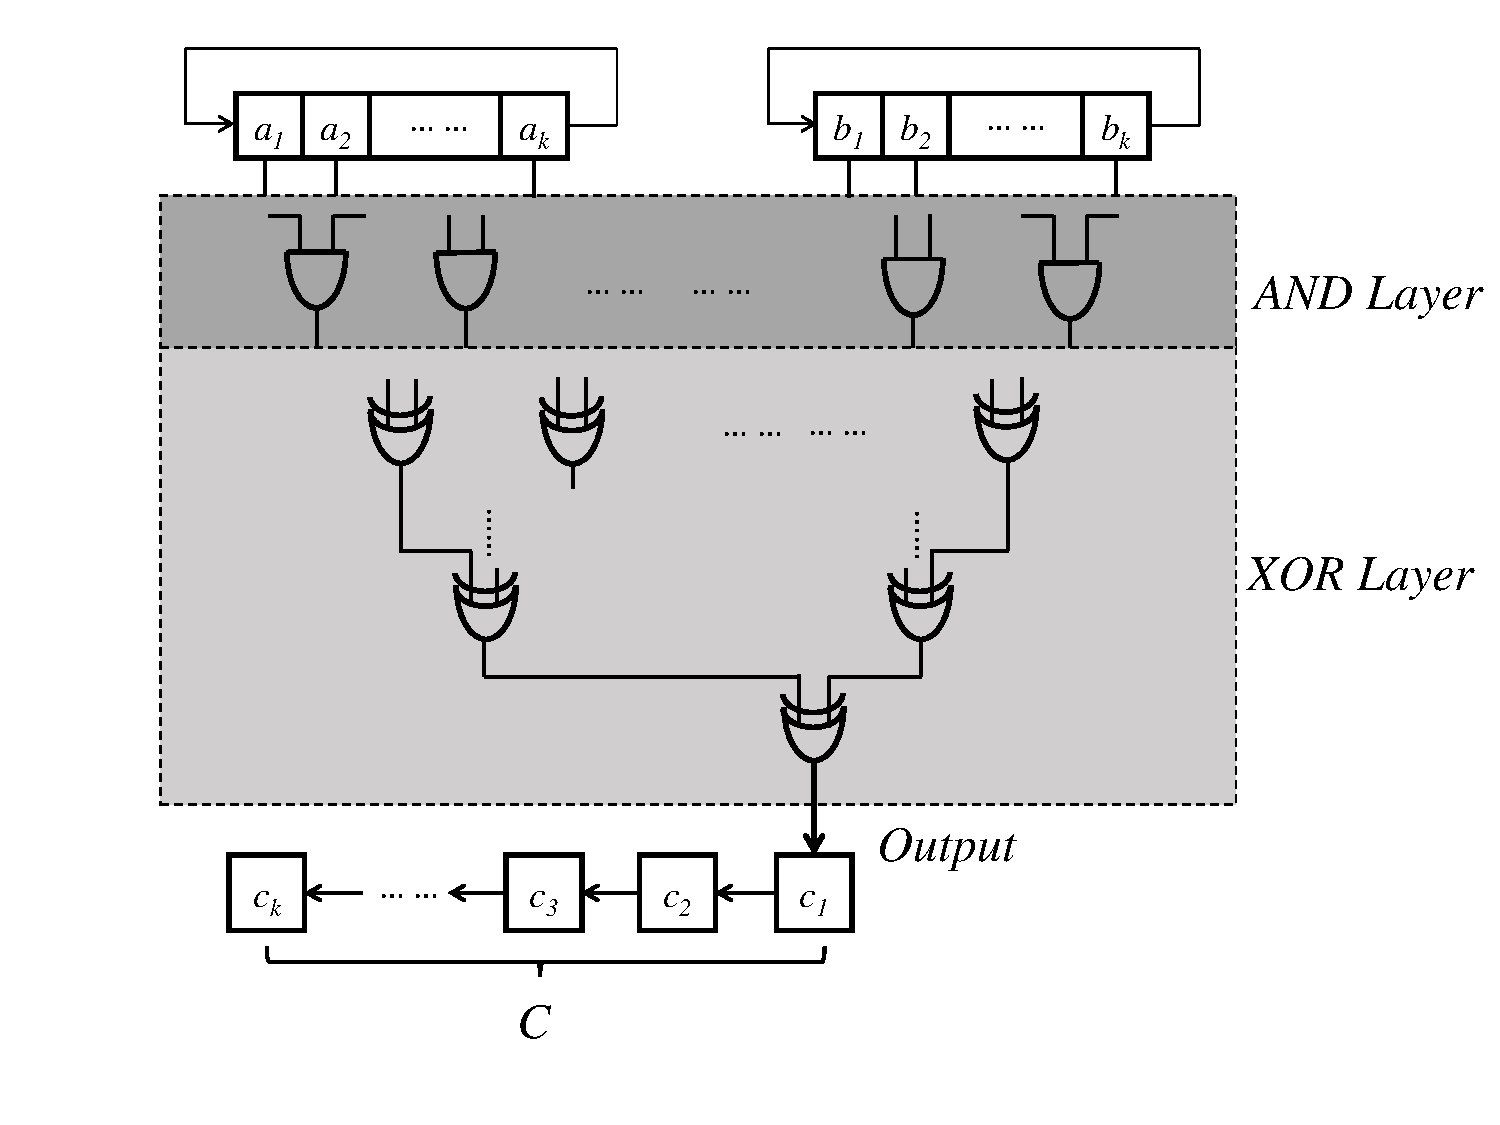
\includegraphics[width=\textwidth]{newfig/MasseyOmura.pdf}
\caption{A typical SMSO structure of Massey-Omura multiplier.}
\label{fig:MasseyOmura}}
\end{figure}

Figure \ref{fig:MasseyOmura} shows the basic architecture of a Massey-Omura multiplier. The operands
$A$ and $B$ are 2 arrays of flip-flops which allow 1-bit right-cyclic shift every clock cycle.
The logic gates in the boxes implements the matrix multiplication with $\lambda$-Matrix $M^{(0)}$, 
while each AND gate corresponds to term $a_ib_j$ and each XOR gate corresponds to addition $a_ib_j+a_{i'}b_{j'}$. 
The XOR layer has only 1 output, giving out 1 bit of product $C$ every clock cycle.

The behavior of Massey-Omura multiplier can be described as: pre-load operands $A,B$ and reset $C$ to 0, after 
executing for $k$ clock cycles, the data stored in flip-flop array $C$ is the product $A\times B$.
We note that there is only one output giving 1 bit of the product each clock cycle, which matches the 
definition of serial output to communication channel. Therefore this type of design is named as 
sequential multiplier with serial output (SMSO).
The SMSO architecture need $C_N$ AND gates and $C_N-1$ XOR gates, which equals to $2k-1$ AND gates and $2k-2$ XOR gates
if it is designed using ONB. In fact, the number of gates can be reduced if the multiplication is 
implemented using a conjugate of SMSO.

The gate-level logic boxes implement the following function:
\begin{equation}
\label{eqn:SMPOterms}
c_l = row_1(A\times M^{(l)}) \times B + row_2(A\times M^{(l)}) \times B + \cdots + row_{k}(A\times M^{(l)}) \times B
\end{equation}
It can be decomposed into $k$ terms. If we only compute one term for each $c_l,~0\leq l\leq k-1$ in one 
clock cycle, make $k$ outputs and add them up using shift register after $k$ clock cycles, 
it will generate the same result with SMSO. This kind of architecture is named as a 
sequential multiplier with parallel outputs (SMPO). The basic SMPO, as a conjugate of Massey-Omura multiplier,
was invented by Agnew {\it et al.} \cite{agnew1991implementation}.

\begin{figure}[H]
\centering{
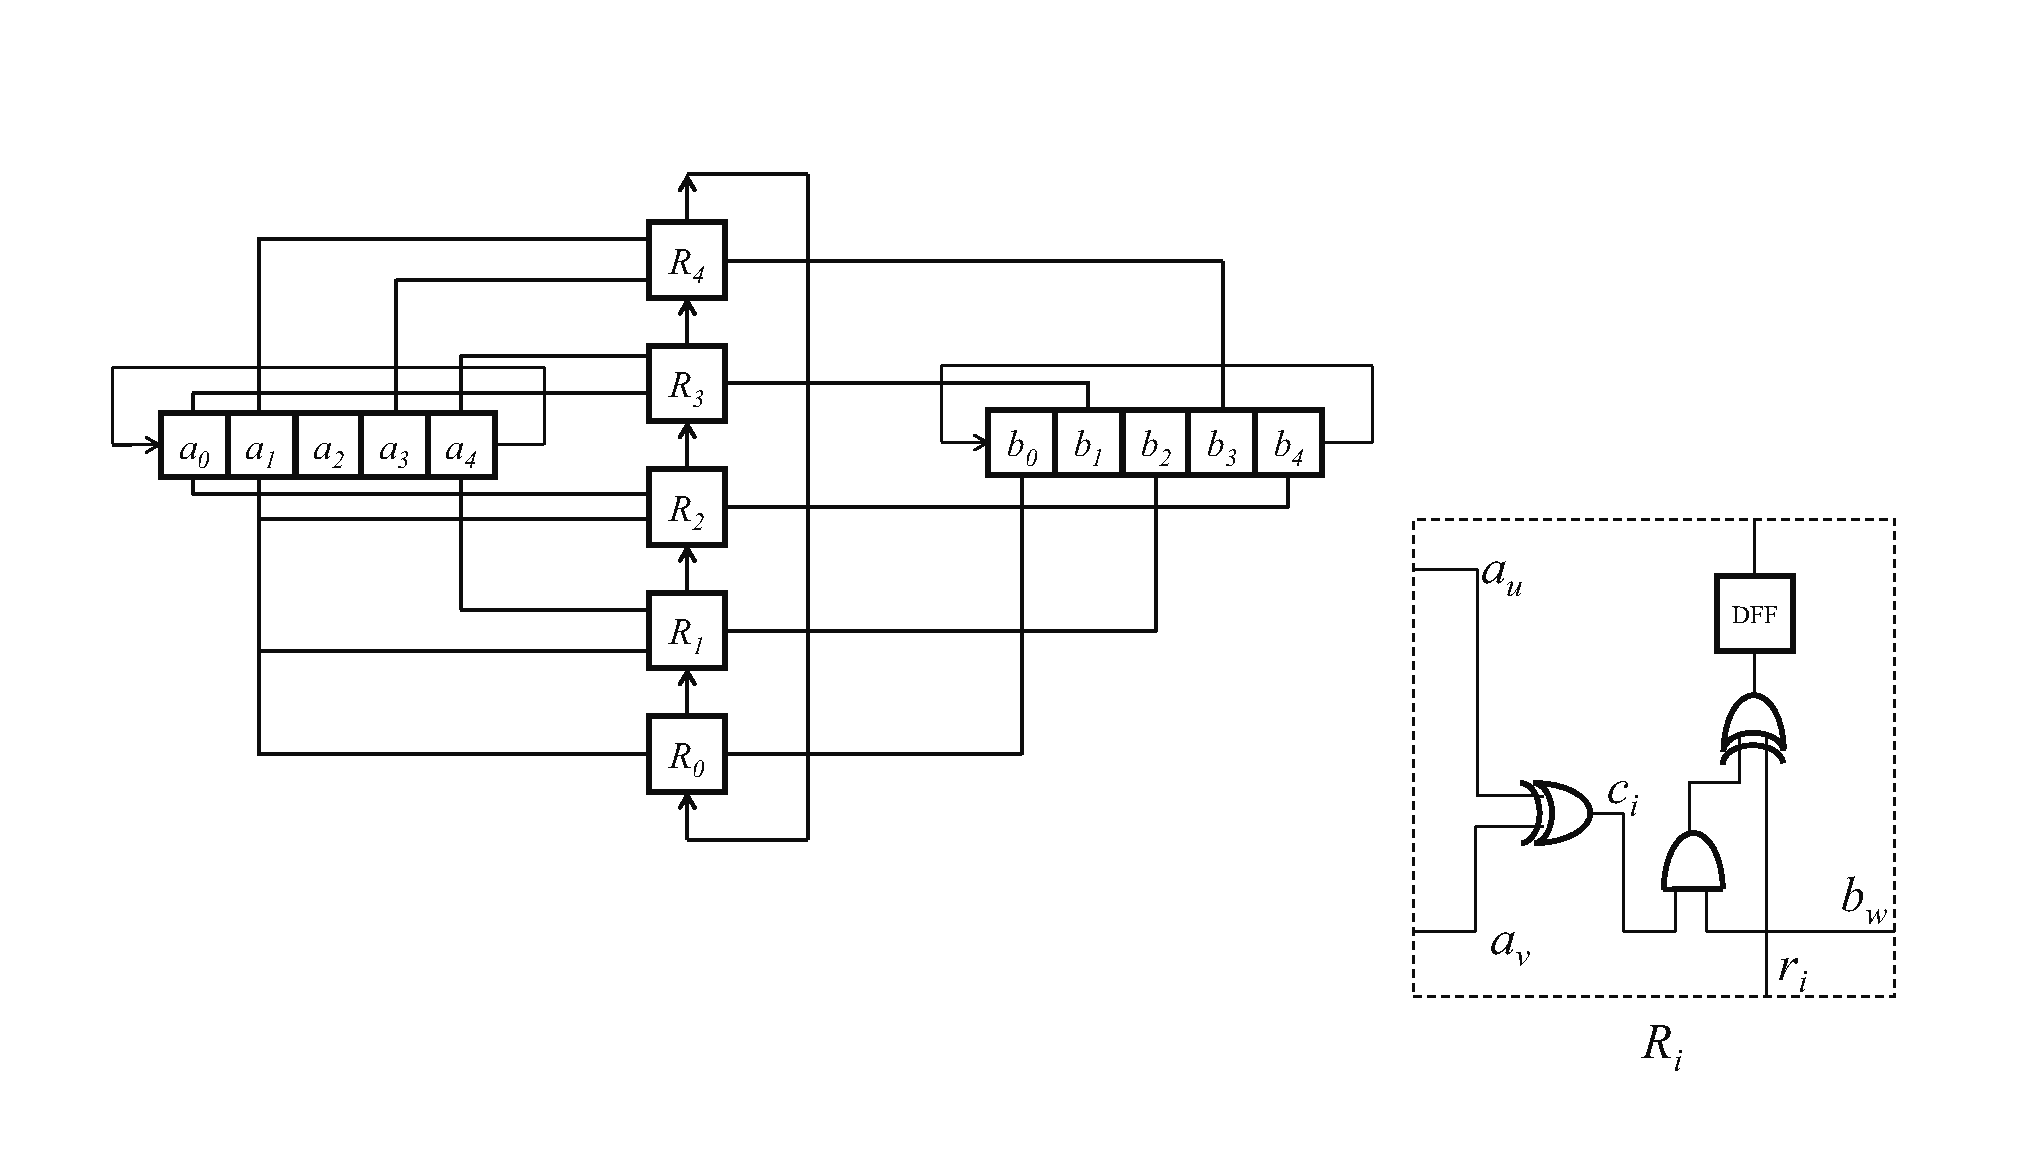
\includegraphics[width=\textwidth]{newfig/mySMPO.eps}
\caption{5-bit Agnew's SMPO. Index $i$ satisfies $0<i<4$, indices $u,v$ are determined by column \# of nonzero entries in $i$-th row of $\lambda$-Matrix $M^{(0)}$, {\it i.e.} if entry $M_{ij}^{(0)}$ is a nonzero entry, $u$ or $v$ equals to $i+j \pmod 5$. Index $w = 2i\pmod 5$.}
\label{fig:SMPO}}
\end{figure}

\begin{Example}[5-bit Agnew's SMPO]
Given GF $\mathbb F_{2^5}$ and primitive element $\alpha$ defined by irreducible polynomial 
$\alpha^5+\alpha^2+1=0$, normal element $\beta = \alpha^5$ constructs an ONB $\{\beta,\beta^2,\beta^4,\beta^8,\beta^{16}\}$.
The $0$-th $\lambda$-Matrix for this ONB is
\begin{equation*}
M^{(0)} = \left(\begin{array}{lcccr}
0 &1 &0 &0 &0 \\
1 &0 &0 &1 &0 \\
0 &0 &0 &1 &1 \\
0 &1 &1 &0 &0 \\
0 &0 &1 &0 &1
\end{array}\right)
\end{equation*}
Then a typical design of 5-bit Agnew's SMPO is depicted in Figure \ref{fig:SMPO}.

The operands part of this circuit is the same with Massey-Omura multiplier. The differences are on 
the matrix multiplication part, while it is implemented as separate logic blocks for 5 outputs,
and the 5 blocks are connected in a shift register fashion. By analyzing the detailed function of 
logic blocks, we can reveal the mechanism of Agnew's SMPO.

Suppose we implement $M^{(0)}$ as the logic block in SMSO. In the first clock cycle, the output is
\begin{equation}
\label{eqn:5bitSMPO_c0}
c_0 = a_1b_0+(a_0+a_3)b_1 + (a_3+a_4)b_2 + (a_1+a_2)b_3 + (a_2+a_4)b_4
\end{equation}
It is written in the form of Equation \ref{eqn:SMPOterms}. In next clock cycles we can obtain 
remaining bits of the product, which can be written in following general form polynomial:
\begin{align}
c_i =& b_ia_{i+1} + b_{i+1}(a_i + a_{i+3}) + b_{i+2}(a_{i+3} + a_{i+4}) \nonumber\\
&+ b_{i+3}(a_{i+1} + a_{i+2}) + b_{i+4}
(a_{i+2} + a_{i+4}),\ 0\leq i\leq 4 \nonumber
\end{align}
Note all index calculations are reduced modulo 5.

Now let us observe the behavior of 5-bit Agnew's SMPO. Initially all DFFs are reset to 0. 
In the first clock cycle,
signal sent to the flip-flop in block $R_0$ denotes function:
$$R_0^{(1)} = a_1b_0$$
It equals to the first term of Equation \ref{eqn:5bitSMPO_c0}. In the second clock cycle,
this signal is sent to block $R_1$ through wire $r_0$, and this block also receives data 
from operands (shifted by 1 bit), generating signal $a_u,a_v$ and $b_w$. Concretely,
signal sent to flip-flop in block $R_1$ is:
$$R_1^{(2)} = R_0^{(1)} + (a_0+a_3)b_1 = a_1b_0+(a_0+a_3)b_1$$
which forms first 2 terms of Equation \ref{eqn:5bitSMPO_c0}. Similarly, we track the signal 
on $R_2$ in third clock cycle, signal on $R_3$ in fourth clock cycle, finally we can get 
$$R_4^{(5)} = a_1b_0+(a_0+a_3)b_1 + (a_3+a_4)b_2 + (a_1+a_2)b_3 + (a_2+a_4)b_4$$
which equals to $c_0$ in Equation \ref{eqn:5bitSMPO_c0}.
After the fifth clock cycle ends, this signal can be detected on wire $r_0$. It shows that 
the result of $c_0$ is computed after 5 clock cycles and given on $r_0$.

If we track $R_1\to R_2\to R_3 \to \cdots \to R_0$, we can obtain $c_1$ respectively.
Thus we conclude that Agnew's SMPO functions the same with Massey-Omura multiplier.
\end{Example}

The design of Agnew's SMPO guarantees that there is only one AND gate in each $R_i$ block.
For ONB, adopting Agnew's SMPO will reduce the number of AND gates from $2k-1$ to $k$.

\subsection{Multiplier not based on the $\lambda$-Matrix}
Both Massey-Omura multiplier and Agnew's SMPO rely on the implementation of $\lambda$-Matrix,
which means that they will be identical if unrolled to full combinational circuits. 
After Agnew's work of parallelization, researchers proposed more designs of SMPO, 
some of them jump out of the box and are independent from $\lambda$-Matrix.
One competitive multiplier design of this type is invented by Reyhani-Masoleh and Hasan 
\cite{RHmulti}, which is therefore called RH-SMPO.

\begin{figure}[H]
\centering{
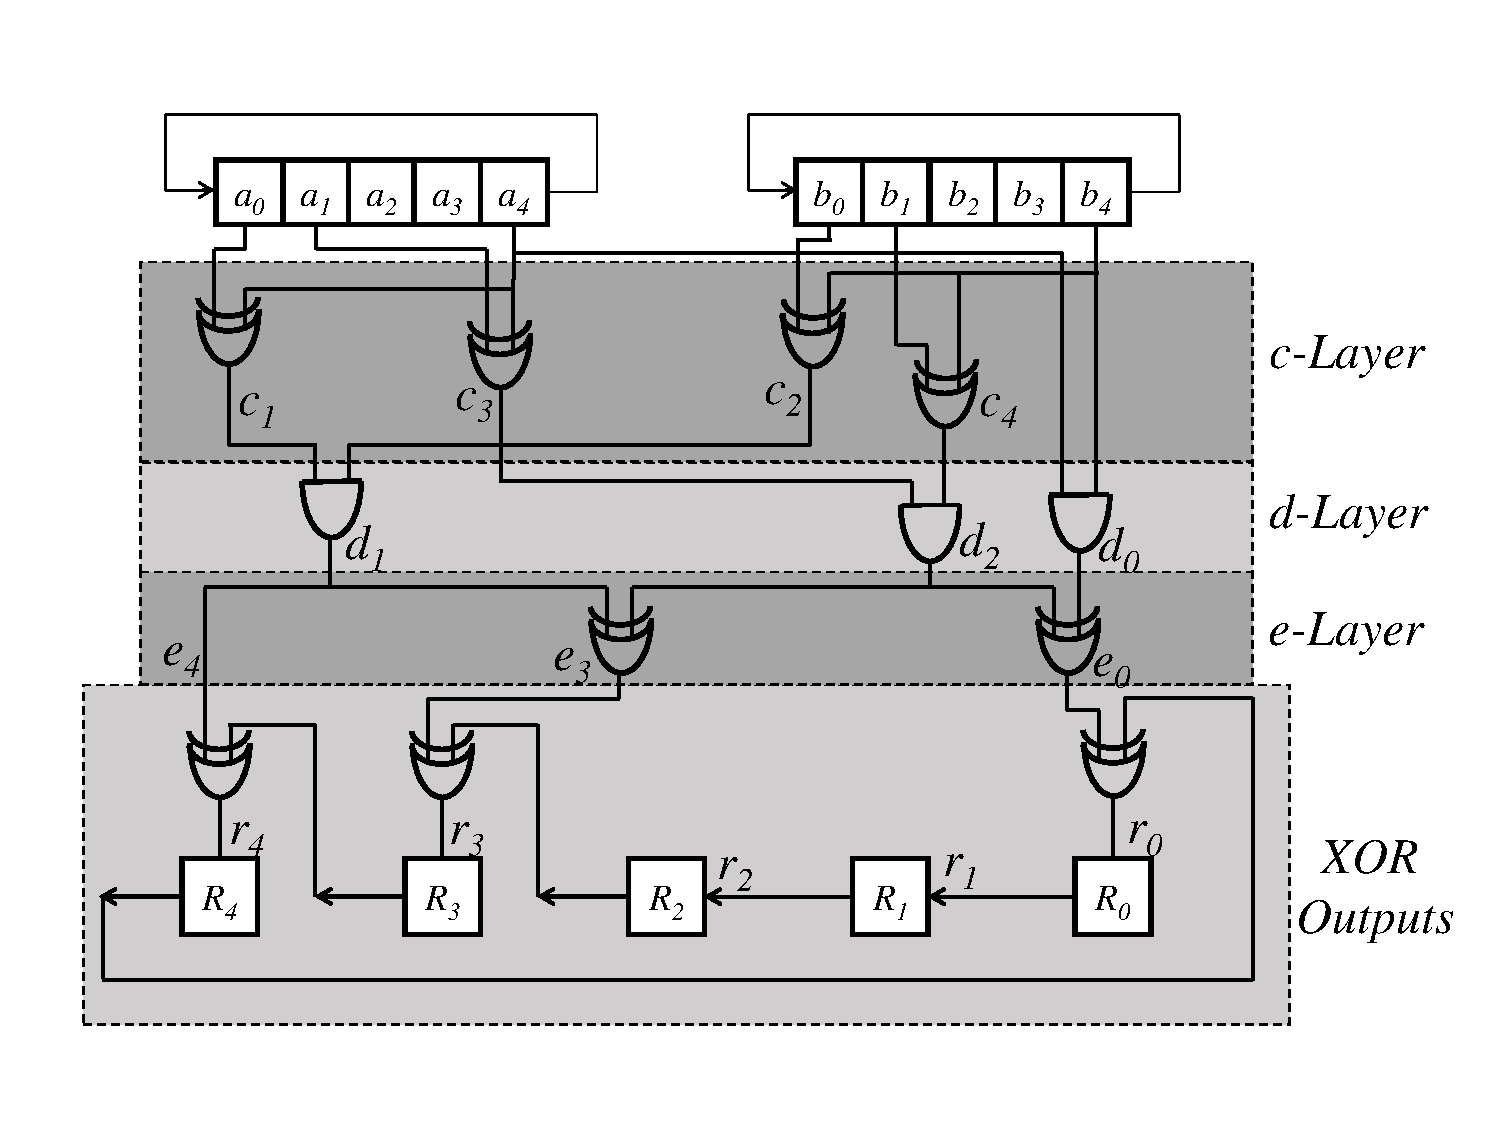
\includegraphics[width=\textwidth]{newfig/5bitRH.pdf}
\caption{A 5-bit RH-SMPO.}
\label{fig:5bitRH}}
\end{figure}

Figure \ref{fig:5bitRH} is a 5-bit RH-SMPO which is functionally equivalent to 5-bit Agnew's SMPO 
in Figure \ref{fig:SMPO}. A brief proof is as follows: 

\begin{Proof}
First, we define an auxiliary function for $i$-th bit 
\begin{equation}
\label{eqn:aux}
F_i(A,B) = a_ib_i\beta + \sum_{j=1}^v d_{i,j}\beta^{1+2^j}
\end{equation}
where $0\leq i\leq k-1, v = \lfloor k/2\rfloor, 1\leq j \leq v$.
The $d$-layer index $d_{i,j}$ is defined as
\begin{equation}
\label{eqn:auxDC}
d_{i,j} = c_{a,i} c_{b,i} = (a_i+a_{i+j})(b_i+b_{i+j}),~~1\leq j\leq v
\end{equation}
$i+j$ here is the result reduced modulo $k$. Note that there is a special boundary case when
$k$ is an even number ($v = \frac{k}{2}$):
$$d_{i,v} = (a_i+a_{i+v})b_i$$
With the auxiliary function, we can utilize following theorem (proof refers to \cite{RHmulti}):
\begin{Theorem}
Consider three elements $A,B$ and $R$ such that $R=A\times B$ over $\Fkk$. Then,
$$R=(((F_{k-1}^2+F_{k-2})^2+F_{k-3})^2+\cdots+F_1)^2+F_0$$
\end{Theorem}
where $F$ is as given in Equation \ref{eqn:aux}.
This form is called inductive sum of squares, and corresponds to the cyclic shifting on 
$R_i$ flip-flops. Concretely, the multiplier behavior is an implementation of 
following algorithm:

\begin{algorithm}[H]
\SetAlgoNoLine

 \KwIn{$A,B\in \Fkk$ given {\it w.r.t.} NB $N$}
 \KwOut{$R=A\times B$}
%%%%%%%%%%%%%%%%%%%%
  Initialize $A,B$ and aux var $X$ to 0\;
  \For { ($i=0$;   $i < k$; ++i ) }
  {
	$X \gets X^2+F_{k-1}(A,B)$ \CommentSty{/*use aux-func from Equation \ref{eqn:aux}*/\;}
	$A\gets A^2,~B\gets B^2$ \CommentSty{/*Right-cyclic shift $A$ and $B$*/\;}
  }
  $R\gets X$
\caption{NB Multiplication Algorithm in RH-SMPO \cite{RHmulti}}\label{alg:RHmulti}
\end{algorithm}

In this algorithm, we use a fixed auxiliary function $F_{k-1}$ inside the loop.
This is because of equation
$$F_{k-l} = F_{k-1}(A^{2^{l-1}},B^{2^{l-1}}),~~1\le l\le k$$
So using fixed $F_{k-1}$ and squaring $A^{2^i}$ every time inside the loop is equivalent to computing 
$F_{k-1},F_{k-2},\dots,F_0$ with fixed operands $A,B$.
\end{Proof}

To better understand the mechanism of RH-SMPO, we will use this 5-bit 
RH-SMPO as an example and introduce the details on how to design it.
\begin{Example}[Designing a 5-bit RH-SMPO]
From Equation \ref{eqn:aux} we can deploy AND gates in $d$-layer according to $d_{i,j}$,
and XOR gates in $c$-layer according to Equation \ref{eqn:auxDC}. Concretely, as Algorithm \ref{alg:RHmulti}
describes, we implement auxiliary function $F_{k-1}$ in the logic:
$$i = k-1 = 4;~~v=\lfloor 5/2 \rfloor = 2$$
\begin{equation}
\label{eqn:5bitRHaux}
F_{4}(A,B) = a_4b_4\beta+\sum_{j=1}^2 d_{4,j}\beta^{1+2^j} = d_0\beta+\sum_{j=1}^2 d_{4,j}\beta^{1+2^j}
\end{equation}
Consider indices $4+1=0\bmod 5,~4+2=1\bmod 5$, write down gates in $c$-layer and $d$-layer (besides $d_0$)
$$c_1 = a_0+a_4,~c_2 = b_0+b_4,~d_1=d_{4,1}= c_1c_2 = (a_4+a_0)(b_4+b_0)$$
$$c_3 = a_1+a_4,~c_4 = b_1+b_4,~d_2=d_{4,2}= c_3c_4 = (a_4+a_1)(b_4+b_1)$$
The difficult part of the whole design is to deploy XOR gates in $e$-layer. 
As the logic layer closest to the outputs $R_i$, $e$-layer actually finishes the implementation of 
$F_{k-1}(A,B)$. But it is not a simple addition; the reason is before bit-wise adding to $X^2$, it is necessary to 
turn the sum to NB form. In other words, theoretically we need $k$ XOR gates in $e$-layer, the output of 
$i$-th gate forms the coefficient of $\beta^{2^i}$.

In order to obtain information 
indicating interconnections between the $d$-layer and $e$-layer, we need to interpret $\beta^{1+2^j}$ 
to NB representation.
There is a concept called {\bf multiplication table} (M-table) which can assist this interpretation. It is defined as 
a $k\times k$ matrix $T$ over $\mathbb F_2$:
\begin{equation}
\label{eqn:multitable}
\begin{bmatrix}
\beta^{1+2^0} \\ \beta^{1+2^1} \\ \beta^{1+2^2} \\ \vdots \\ \beta^{1+2^{k-1}}
\end{bmatrix}
= \beta
\begin{bmatrix}
\beta \\ \beta^2 \\ \beta^4 \\ \vdots \\ \beta^{2^{k-1}}
\end{bmatrix}
=
\begin{bmatrix}
T_{0,0}      &   T_{0,1}        & \dots & T_{0,k-1}\\
T_{1,0}    &   T_{1,1}           & \dots & T_{1,k-1}\\
T_{2,0}    &   T_{2,1}           & \dots & T_{2,k-1}\\
\vdots & \vdots              & \ddots     & \vdots \\
T_{k-1,0}    &   T_{k-1,1}           & \dots & T_{k-1,k-1}
\end{bmatrix}
\begin{bmatrix}
\beta \\ \beta^2 \\ \beta^4 \\ \vdots \\ \beta^{2^{k-1}}
\end{bmatrix}
= {\bf T}
\begin{bmatrix}
\beta \\ \beta^2 \\ \beta^4 \\ \vdots \\ \beta^{2^{k-1}}
\end{bmatrix}
\end{equation}

It is a known fact that M-table $T$ can be converted from $\lambda$-Matrix $M$:
$$M_{i,j}^{(0)} = T_{j-i,-i}$$
with indices reduced modulo $k$ (proof given in Appendix \ref{append:ONB}). Thus we can write down the M-table of $\mathbb F_{2^5}$ with current NB $N$:

\begin{figure}[H]
\centering{
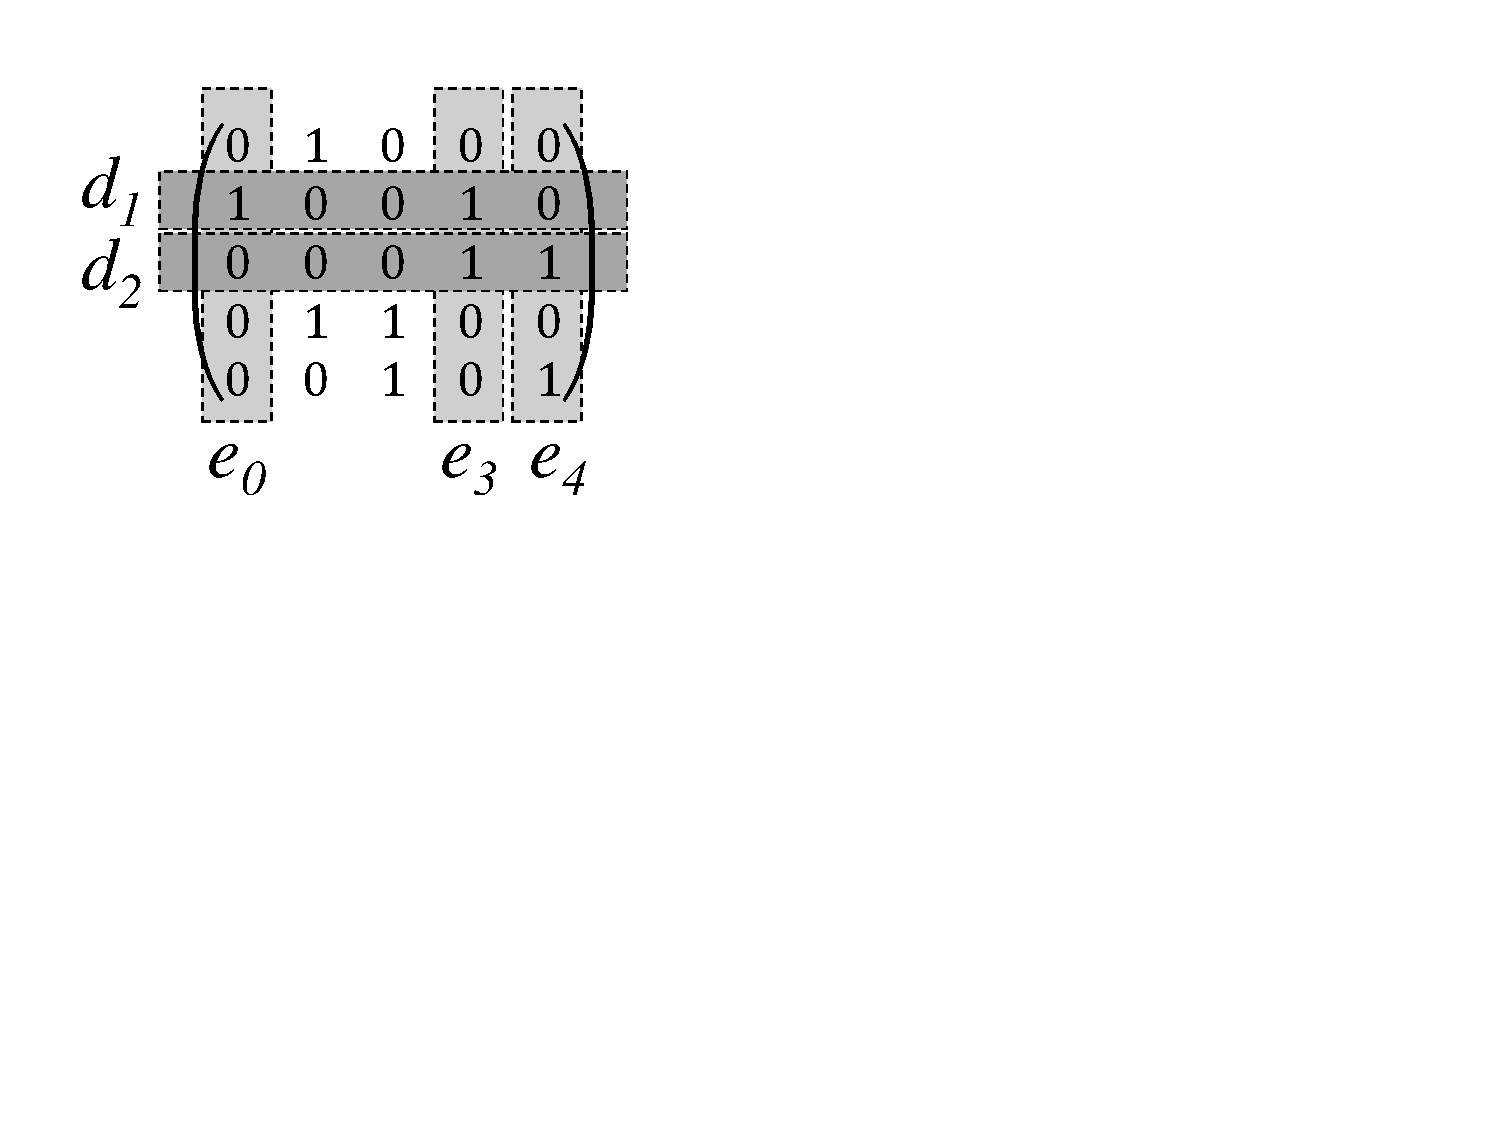
\includegraphics[width=3in]{newfig/multitable.pdf}
\caption{A $5\times 5$ multiplication table.}
\label{fig:multitable}}
\end{figure}

Note that we only use row 1 and row 2 from the M-table since range $1\leq j \leq 2$.
All nonzero entries in these 2 rows corresponds to the interconnections between $d$-layer and 
$e$-layer. For example, row 1 has two nonzero entries at column 0 and column 3, which corresponds to interconnections 
between $d_1$ and $e_0,e_3$. This conclusion comes from row 1 in Equation \ref{eqn:multitable}:
\begin{equation*}
\beta\cdot\beta^2 = 
\begin{bmatrix}
1 & 0 & 0 & 1 & 0
\end{bmatrix}
\begin{bmatrix}
\beta \\ \beta^2 \\ \beta^4 \\ \beta^8 \\ \beta^{16}
\end{bmatrix}
= \beta + \beta^{2^3}
\end{equation*}

Similarly, from row 2 of M-table we derive that $d_2$ has fanouts $e_3,e_4$:
\begin{equation*}
\beta\cdot\beta^{2^2} = 
\begin{bmatrix}
0 & 0 & 0 & 1 & 1
\end{bmatrix}
\begin{bmatrix}
\beta \\ \beta^2 \\ \beta^4 \\ \beta^8 \\ \beta^{16}
\end{bmatrix}
= \beta^{2^3} + \beta^{2^4}
\end{equation*}

Let us look back at Equation \ref{eqn:5bitRHaux}, we already dealt with the latter part.
The first term is always $d_0\beta$, which denotes $d_0$ should always be connected to $e_0(\beta)$.
After gathering all interconnection information, we can translate it to gate-level circuit implementation:
$$e_0 = d_0+d_1,~e_3=d_1+d_2,~e_4=d_2$$

Then the last mission is to implement the output $R_i$ layer. Assume $r_{i-1}$ is the output of 
$R_{i-1}$ in last clock cycle, we can connect using relation 
$$R_i = r_{i-1} + e_i$$
In this example, according to the M-table in Figure \ref{fig:multitable}, columns $e_1,e_2$
have only zeros in its intersection with row $d_1,d_2$. Thus gates for $e_1,e_2$ can be omitted.

This finishes the full design procedure for a 5-bit RH-SMPO.
\end{Example}

The area cost of RH-SMPO is even smaller than Agnew's SMPO. XOR gates corresponds to all nonzero entries 
in M-table, which is with the same number of nonzero entries in $\lambda$-Matrix ($C_N$). The number of AND gates 
equals to $v$ plus 1 (for gate $d_0$). When using ONB ($C_N = 2k-1$), the total number of gates 
is $2k+\lfloor \frac{k}{2}\rfloor$.

\section{Concluding Remarks}
In this chapter, we introduced basic concepts such as the definition of finite fields and the construction 
of finite fields. Moreover, we described a special kind of basis in finite field, and its 
application on Galois field hardware design. The sequential Galois field multipliers based on these 
principles are used as candidates for applying our functional verification approach in subsequent chapters.
\chapter{Gr\"ober Bases and Algebraic Geometry} \label{ch:ideals}
This chapter reviews fundamental concepts of commutative and 
computer algebra which are used in this work. 
Specifically, this chapter covers monomial ordering, polynomial ideals and 
varieties, and the computation of \Grobner bases.
It also overviews elimination theory as well as Hilbert's Nullstellensatz 
theorems and how
they apply to Galois fields. The results of these theorems are used in polynomial
abstraction and formal verification of Galois field circuits and 
are discussed 
in subsequent chapters. The material of this chapter is
mostly taken from the textbooks \cite{ideals:book,gb_book} and 
previous work by Lv \cite{lv:phd} as well as Pruss \cite{pruss:tcad15}.

\section{Algebraic Geometry Fundamentals}
\label{sec:geo}
\subsection{Monomials, Polynomials and Polynomial Algebra}
\begin{Definition} \label{def:mono}
A {\bf monomial} in variables $x_1,x_2,\cdots,x_d$ is a product of the form:
\begin{equation}
x_1^{{\alpha}_1} \cdot x_2^{{\alpha}_2} \cdot \cdots x_d^{{\alpha}_d},
\end{equation}
where $\alpha_i \ge 0, i\in\{1,\cdots,d\}$. 
The total degree of the monomial is $\alpha_{1}+\cdots+\alpha_{d}$.
\end{Definition} 

Thus, $x^2\cdot y$ is a monomial in variables $x,y$ with total degree $3$.
For simplicity, we will henceforth denote a 
monomial $x_1^{{\alpha}_1} \cdot x_2^
{{\alpha}_2} \cdot \cdots x_d^{{\alpha}_d}$ as $x^{\alpha}$, 
where $\alpha=({\alpha}_1,\cdots,{\alpha}_d)$ is a vector size $d$ of 
integers $\ge 0$, i.e., $\alpha \in \mathbb{Z}_{\ge 0}^{d}$.

\begin{Definition}\label{def:poly}
Let $\mathbb{R}$ be a ring. A {\bf polynomial} over $\mathbb{R}$ in the 
indeterminate $x$ is an expression of the form:
\begin{equation} \label{eq:poly1}
a_0 + a_1 x + a_2 x^2 + \cdots + a_k x^k = \sum_{i=0}^{k} a_i x^i, \forall a_i \in \mathbb{R}. 
\end{equation}

\end{Definition}

The constants $a_i$ are the coefficients and $k$ is the degree of the polynomial. 
For example, $8x^3 + 6x + 1$ is a polynomial in $x$ over $\mathbb{Z}$, with
coefficients $8$, $6$, and $1$ and degree $3$. 

\begin{Definition}
The set of all polynomials in the indeterminate
$x$ with coefficients in the ring $\mathbb{R}$ forms a {\bf
ring of polynomials} $\mathbb{R}[x]$. 
Similarly, $\mathbb{R}[x_1,x_{2},\cdots, x_{n}]$ 
represents the ring of multivariate polynomials with coefficients in $\mathbb{R}$.
\end{Definition}

For example, $\mathbb{Z}_{2^4}[x]$ stands for the set of all polynomials in
$x$ with coefficients in $\mathbb{Z}_{2^4}$. $8x^3 + 6x + 1$ is an instance 
of a polynomial contained in $\mathbb{Z}_{2^4}[x]$.

\begin{Definition}
A {\bf multivariate polynomial} $f$ in variables $x_1, x_2, \ldots, x_d$ 
with coefficients in any given field $\F$ is a finite linear 
combination of monomials with coefficients in $\F$: 
\begin{equation}
	f=\sum_{\alpha}a_{\alpha}\cdot x^{\alpha}, ~~a_{\alpha}\in \F \nonumber
\end{equation}

The set of all polynomials in $x_1, x_2, \ldots, x_d$ with coefficients in 
field $\F$ is denoted by $\F[x_1, x_2, \ldots, x_d]$. 
Thus, $f \in \F[x_1, x_2, \ldots, x_d]$

\begin{enumerate}
\item We refer to the constant $a_{\alpha} \in \F$ as the 
{\bf coefficient} of the monomial $a_{\alpha} x^{\alpha}$.
\item If $a_{\alpha} \neq 0$, we call $a_{\alpha} x^{\alpha}$ a term of $f$.
\end{enumerate}
\end{Definition}

As an example, $2x^2+y$ is a polynomial with two terms $2x^2$ and $y$, with 
$2$ and $1$ as coefficients respectively. 
In contrast, $x+y^{-1}$ is not a polynomial because the exponent of $y$ is 
less than $0$.

Since a polynomial is a sum of its terms,
these terms have to be arranged unambiguously so that they can be 
manipulated in a consistent manner.
Therefore, we need to establish a concept of 
{\bf term ordering} (also called monomial ordering).
A term ordering, represented by $>$, defines how
terms in a polynomial are ordered.

Common term orderings are lexicographic ordering (LEX) and its variants: 
degree-lexicographic ordering (DEGLEX) and reverse degree-lexicographic ordering (DEGREVLEX).

A {\bf lexicographic ordering} (LEX) is a total-ordering $>$ such that 
variables in the terms are lexicographically ordered, {\it i.e.} simply based on 
when the variables appear in the ordering. It is also a well-order, where the least element exists.
Higher variable-degrees take 
precedence over lower degrees for equivalent variables ({\it e.g.} $a^3 > a^2$ due to $a \cdot a \cdot a > a \cdot a \cdot 1$).
\begin{Definition}
{\bf Lexicographic order:} Let $x_1 > x_2 > \dots > x_d$
lexicographically. Also let $\alpha = (\alpha_1, \dots, \alpha_d);
~\beta = (\beta_1, \dots, \beta_d) \in \mathbb{Z}^d_{\geq 0}$. Then we
have: 
\begin{equation}
x^{\alpha} > x^{\beta} \iff 
\begin{cases}
& \text{Starting  from the  left, the first co-ordinates of $\alpha_i, \beta_i$} \\
& \text{that are different satisfy $\alpha_i > \beta_i$}

\end{cases}
\end{equation}
\end{Definition}

A {\bf degree-lexicographic ordering} (DEGLEX) is a total-ordering $>$ such 
that the total degree of a term takes precedence over the lexicographic 
ordering.  
A {\bf degree-reverse-lexicographic ordering} (DEGREVLEX) is the same as a
DEGLEX ordering, but terms are LEXed in reverse.

\begin{Definition}
{\bf Degree Lexicographic order:} Let $x_1 > x_2 > \dots > x_d$
lexicographically. Also let $\alpha = (\alpha_1, \dots, \alpha_d);
~\beta = (\beta_1, \dots, \beta_d) \in \mathbb{Z}^d_{\geq 0}$. Then we
have: 
\begin{equation}
x^{\alpha} > x^{\beta} \iff 
\begin{cases}
\sum_{i=1}^{d}\alpha_i > \sum_{i=1}^{d} \beta_i & \text{ or }\\
\sum_{i=1}^{d}\alpha_i = \sum_{i=1}^{d} \beta_i  \text{ and }
x^{\alpha} > x^{\beta} & \textit{w.r.t.}\text{ LEX order}
\end{cases}
\end{equation}
\end{Definition}


\begin{Definition}
{\bf Degree Reverse Lexicographic order:} Let $x_1 > x_2 > \dots > x_d$
lexicographically. Also let $\alpha = (\alpha_1, \dots, \alpha_d);
~\beta = (\beta_1, \dots, \beta_d) \in \mathbb{Z}^d_{\geq 0}$. Then we
have: 
\begin{equation}
x^{\alpha} > x^{\beta} \iff 
\begin{cases}
\sum_{i=1}^{d}\alpha_i > \sum_{i=1}^{d} \beta_i  \text{ or }\\
\sum_{i=1}^{d}\alpha_i = \sum_{i=1}^{d} \beta_i  \text{ and the first co-ordinates}\\
\text{$\alpha_i, \beta_i$ from the right, which are different, satisfy $\alpha_i < \beta_i$}
\end{cases}
\end{equation}

\end{Definition}

Based on the {\it monomial ordering}, we have the following concepts:

\begin{Definition}
The {\bf leading term} is the first term in a term-ordered polynomial.
Likewise, the {\bf leading coefficient} is the coefficient of
the leading term. 
Finally, a {\bf leading monomial} is the leading term 
lacking the coefficient.  We use the following notation:
\begin{eqnarray}
     lt(f)&& \text{Leading Term} \\
     lc(f)&& \text{Leading Coefficient} \\
     lm(f)&& \text{Leading Monomial} \\
     tail(f)&& f - lt(f)
\end{eqnarray}
\end{Definition}

\begin{Example}
\begin{eqnarray}
     f      &=& 3a^2b + 2ab + 4bc \\
     lt(f)  &=& 3a^2b \\
     lc(f)  &=& 3 \\
     lm(f)  &=& a^2b \\
     tail(f) &=& 2ab+4bc
\end{eqnarray}
\end{Example}

{\bf Polynomial division} is an operation over polynomials that is dependent on
the imposed monomial ordering. Dividing a polynomial $f$ by another polynomial
$g$ cancels the leading term of $f$ to derive a new polynomial. 

\begin{Definition}
Let $\F$ be a field and let $f, g \in \F[x_1, x_2, \ldots, x_d]$ be polynomials
over the field. {\bf Polynomial division} of $f$ by $g$ is computed following:
\begin{equation}
f-\frac{lt(f)}{lt(g)}\cdot g
\end{equation}
This polynomial division is denoted
\begin{equation}
f\xrightarrow{g} r
\end{equation}
where $r$ is the resulting polynomial of the division.
If $\frac{lt(f)}{lt(g)}$ is nonzero, then $f$ is considered divisible by $g$, 
{\it i.e.}, $g \mid f$.
\end{Definition}
Notice that if $g \nmid f$, that is if $f$ is not divisible by $g$,
then the division operation gives $r = f$.
\begin{Example}
Over $\R[x,y,z]$, set the lex term order $x > y > z$.
Let $f = -2x^3 + 2x^2yz + 3xy^3$ and $g = x^2+yz$.
\begin{equation}
\frac{lt(f)}{lt(g)} = \frac{-2x^3}{x^2} = -2x
\end{equation}
Since $\frac{lt(f)}{lt(g)}$ is nonzero $g|f$. The division, $f\xrightarrow{g} r$, 
is computed as:
\begin{eqnarray}
r &=& f-\frac{lt(f)}{lt(g)}\cdot g = -2x^3 + 2x^2yz + 3xy^3 - (-2x \cdot (x^2+yz)) \nonumber \\
&=& -2x^3 + 2x^2yz + 3xy^3 - (-2x^3-2xyz) = 2x^2yz + 3xy^3 + 2xyz
\end{eqnarray}
Notice that the division $f\stackrel{g}{\textstyle\longrightarrow}r$ cancels the leading term of $f$.
\end{Example}

Similarly, we can also define when a polynomial is divided (reduced) by a set of polynomials.
\begin{Definition}
    The {\bf reduction} of a polynomial $f$, by another polynomial $g$, to
    a reduced polynomial $r$ is denoted:
    \begin{equation*}
        f\stackrel{g}{\textstyle\longrightarrow}_{+}r
    \end{equation*}
    which is the transitive and reflective closure of the relation $f\stackrel{g}{\textstyle\longrightarrow}r$. 
    Reduction is carried out using multivariate, polynomial long division. 
    % The long division is performed according to a term-ordering on polynomials, and the division algorithm 
    %terminates when the leading term of the divisor does not divide any 
    %other term in the dividend.
  
    For sets of polynomials, the notation 
    \begin{equation*}
    f\stackrel{F}{\textstyle\longrightarrow}_+r    
    \end{equation*}
    represents the reduced polynomial $r$ resulting from $f$ as reduced by a 
    set of nonzero polynomials $F = \{f_1,\dots,f_s\}$.  The polynomial $r$ is considered {\bf reduced} if 
    $r = 0$  or no term in $r$ is divisible  by $lm(f_i), \forall f_i \in F$.
\end{Definition}

The reduction process $f\stackrel{F}{\textstyle\longrightarrow}_+r$, of 
dividing a polynomial $f$ by a set of polynomials of $F$, can be modeled as
repeated long-division of $f$ by each of the polynomials in $F$ until no
further reductions can be made. The result of this process is then $r$.
This reduction process is shown in Algorithm \ref{alg:polydiv}.

\begin{algorithm}[H]
\SetAlgoNoLine
\LinesNumbered
 \KwIn{$f,f_{1},\dots,f_{s}$}
 \KwOut{$r,a_{1},\dots,a_{s}$, such that $f=a_{1}\cdot f_{1}+\dots+a_{s}\cdot f_{s}+r$.}
 
 $a_{1}=a_{2}=\dots=a_{s}=0$; $r=0$\;
 $p:=f$\;
 
 \While { $p \neq 0$ }
 {
	i=1\;
	divisionmark = false\;
	\While { $i\le s  $ \&\& divisionmark = false }
	{
		\eIf {$f_{i}$ can divide $p$}
		{
			$a_{i}=a_{i}+lt(p)/lt(f_{i})$\;
			$p=p-lt(p)/lt(f_{i}) \cdot f_{i}$\;
			divisionmark = true\;
		}
		{
			i=i+1\;
		}
	}
	
	\If {divisionmark = false}
	{
		$r=r+lt(p)$\;
		$p=p-lt(p)$\;
	}

 }
\caption{Polynomial Reduction}\label{alg:polydiv}
\end{algorithm}

The reduction algorithm keeps canceling the leading terms of polynomials 
until no more leading terms can be further canceled.
So the key step is $p=p-lt(p)/lt(f_{i}) \cdot f_{i}$, as the following 
example shows.
\begin{Example}
Given $f = y^{2}-x$ and $f_{1} = y - x$ in $\mathbb{Q}[x,y]$ with $deglex$: 
$y>x$, perform $f\stackrel{f_1}{\textstyle\longrightarrow}_+r$:

\begin{enumerate}
\item $f=y^{2}-x$, $f/f_{1}=f-lt(f)/lt(f_{1}) \cdot f_{1}=y^{2}-x-(y^{2} /y) \cdot (y-x)=y\cdot x-x$
\item $f=y\cdot x-x$, $f/f_{1}=f-lt(f)/lt(f_{1}) \cdot f_{1}=(y\cdot x-x)/f_{1}=x^{2}-x$
\item $f=x^{2}-x$, no more operations possible, so $r=x^{2}-x$
\end{enumerate}
\end{Example}

\subsection{Varieties and Ideals}
%%%%%%%%%%%%%%%%%%%%%%%%%%%%%%%%%%%%%%%%%%%%%%%%%%%%%%%%%%%%%%%%%%%%%%%%%%%%
%%%%%%%%%%%%%%%%%%%%%  variety %%%%%%%%%%%%%%%%%%%%%%%%%%%%%%%%%%%%%%%%%%
In computer-algebra-based formal verification,
it is often necessary to analyze the presence 
or absence of solutions to a given system of constraints.
In our applications, these constraints are polynomials and their solutions 
are modeled as {\bf varieties}.

\begin{Definition}
Let $\F$ be a field, and let $f_1, \ldots, f_s 
\in \F[x_1, x_2, \ldots, x_d]$. 
We call $V(f_1, \dots, f_s)$ the {\bf affine variety} 
defined by $f_1, \dots, f_s$ as:
\begin{equation}
V(f_1, \ldots, f_s)= \{(a_1, \ldots, a_{d})\in \F^d:f_i(a_1, \ldots, a_d)=0, \forall{i},1\le i \le s\}
\end{equation}
\end{Definition}

$V(f_1, \dots, f_s)\in \F^d$ is {\bf the set of all solutions} in $\F^d$ 
of the system of equations: 
$f_1(x_1,\ldots,x_d)=\dots=f_s(x_1,\dots,x_d)=0$. 

\begin{Example}
Given $\mathbb{R}\left[x,y\right]$, $V(x^2+y^2)$ is the set of all elements
that satisfy $x^2+y^2=0$ over $\mathbb{R}^2$. So $V(x^2+y^2)=\{(0,0)\}$. 
Similarly, in $\mathbb{R}\left[x,y\right]$, $V(x^2+y^2-1)=\{all\  points\  on\ the\ circle: x^2+y^2-1=0\}$.
Note that varieties depend on which field we are operating on. 
For the same polynomial $x^2+1$, we have:
\begin{itemize}
\item In $\mathbb{R}[x]$, $V(x^2+1)=\emptyset$.
\item In $\mathbb{C}[x]$, $V(x^2+1)=\{(\pm i)\}$.
\end{itemize}
\end{Example}

The above example shows the variety can be infinite, finite (nonempty set) 
or empty. It is interesting to note that since we will be operating over
finite fields $\F_{q}$, any finite set of points is a variety. Likewise,
any variety over $\F_{q}$ is finite (or empty).
Consider the points $\{(a_1,\dots, a_d): a_1, \dots, a_d \in \F_q\}$
in $\F_q^d$. Any single point is a variety of some polynomial system:
{\it e.g.} $(a_1,\dots, a_d)$ is a variety of $x_1-a_1 = x_2 - a_2 = \dots =
x_d-a_d=0$. {\bf Finite unions} and {\bf finite  intersections} of
varieties are also varieties. 

\begin{Example}
Let $U = V(f_1, \dots, f_s)$ and $W =
V(g_1, \dots, g_t)$ in $\F_{q}$. Then:  
\begin{itemize}
\item $U \cap W = V(f_1, \dots, f_s, g_1, \dots, g_t)$
\item $U \cup W = V(f_i g_j: 1 \leq i \leq s, 1 \leq j \leq t)$
\end{itemize}
\end{Example}

One important distinction we need to make about varieties is that a
variety depends not just on the given system of polynomial 
equations, but rather on the {\bf ideal} generated by the polynomials.

%%%%%%%%%%%%%%%%%%%%%  ideal %%%%%%%%%%%%%%%%%%%%%%%%%%%%%%%%%%%%%%%%%%
\begin{Definition} 
A subset $I \subset \F[x_1, x_2, \ldots, x_d]$ is an {
\bf ideal} if it satisfies:
\begin{itemize}
\item $0 \in I$
\item $I$ is closed under addition: $x, y \in I \Rightarrow x+y \in I$
\item If $x \in \F[x_1, x_2, \ldots, x_d]$ and $y \in I$, then $x\cdot y \in I$ and $y\cdot x \in  I$.
\end{itemize}
\end{Definition}

An ideal is generated by its {\it basis} or {\it generators}.

%%%%%%%%%%%%%%%%%%%%%  ideal basis%%%%%%%%%%%%%%%%%%%%%%%%%%%%%%%%%%
\begin{Definition}
Let $f_1, f_2, \ldots, f_s$ be 
polynomials of the ring $\F[x_1, x_2, \ldots, x_d]$. 
Let $I$ be an ideal generated by $f_1, f_2, \ldots, f_s$. Then:
\begin{equation}
I = \langle f_1,\dots,f_s \rangle=\{h_1 f_1 + h_2 f_2 + \ldots + h_s f_s : h_1,\dots,h_s\in\F[x_1, \dots, x_d]\} \nonumber
\end{equation}
then, $f_1, \ldots, f_s$ are called the {\bf basis (or generators)} of the 
ideal $I$ and correspondingly $I$ is denoted as $I = \langle f_1, f_2, 
\ldots, f_s \rangle$. 
\end{Definition}

\begin{Example}
The set of even integers, which is a subset of the ring of integers
$Z$, forms an ideal of $Z$. This can be seen from the following;
\begin{itemize}
\item $0$ belongs to the set of even integers.
\item The sum of two even integers $x$ and $y$ is always an even
  integer.
\item The product of any integer $x$ with an even integer $y$ is
  always an even integer.
\end{itemize}
\end{Example}

\begin{Example}
Given $\mathbb{R}\left[x,y\right]$, $I = \langle x, y \rangle$ is an 
ideal containing all polynomials generated by $x$ and $y$, 
such as $x^2+y$ and $x+x\cdot y$. The ideal
$J = \langle x^2, y^2 \rangle$ is an ideal containing all polynomials 
generated by $x^2$ and $y^2$, such as $x^2+y^3$ and $x^{10}+x^2\cdot y^2$. 
Notice that $J\subset I$ because every polynomial generated by $J$ can
be generated by $I$. 
But $I\neq J$ because $x+y$ can only be generated by $I$.
\end{Example}

The same ideal may have many different bases.
For instance, it is possible to have different sets of polynomials
$\{f_1,\dots,f_{s}\}$ and $\{g_{1},\dots,g_{t}\}$ that may generate the same 
ideal, i.e., $\langle f_{1},\dots,f_{s}\rangle=\langle g_{1},\dots,g_{t}\rangle$. Since 
variety depends on the ideal, these sets of polynomials have the same 
solutions.

\begin{Proposition}
If $f_1,\dots,f_{s}$ and $g_{1},\dots,g_{t}$ are bases of the same ideal 
in $\mathbb{F}[x_{1},\dots,x_{d}]$,
so that $\langle f_{1},\dots,f_{s}\rangle=\langle g_{1},\dots,g_{t}\rangle$, 
then $V(f_{1},\dots,f_{s})=V(g_{1},\dots,g_{t})$.
\end{Proposition}

\begin{Example}
	Consider the two bases $F_{1}=\{(2x^{2}+3y^{2}-11,x^{2}-y^{2}-3\}$ and $F_{2}=\{x^{2}-4,y^{2}-1\}$.
	These two bases generate the same ideal, i.e., $\langle F_{1}\rangle= \langle F_{2} \rangle$.{}
	Therefore, they represent the same variety, i.e., 
	\begin{equation}
		V(F_{1})= V( F_{2})=\{\pm 2, \pm 1\}.
	\end{equation}
\end{Example}

Ideals and their varieties are a key part of computer-algebra-based formal
verification. A given hardware design can be transformed into a set
of polynomials over a field, $F = \{f_1, \ldots, f_s\}$.
This set of polynomials gives the system of equations:
\begin{eqnarray}
f_1 = 0 \nonumber \\
\vdots \nonumber \\
f_s = 0 \nonumber
\end{eqnarray}
Using algebra, it is possible to derive new equations from the original 
system.
The ideal $\langle f_1,\ldots, f_s \rangle$ provides a way of analyzing 
such {\it consequences} of a system of polynomials.

\begin{Example}
Given two equations in $\mathbb{R}[x,y,z]$:
\begin{eqnarray}
x=z+1 \nonumber \\
y=x^2+1 \nonumber 
\end{eqnarray}
we can eliminate $x$ to obtain a new equation:
\begin{equation}
y=(z+1)^2+1=z^2+2z+2 \nonumber 
\end{equation}
Let $f_1, f_2, h \in \mathbb{R}[x,y,z]$ be polynomials based on these 
equations:
\begin{eqnarray}
f_1 &= x-z-1 &= 0 \nonumber \\
f_2 &= y-x^2-1 &= 0 \nonumber \\
h   &= y-z^2-2z-2 &= 0 \nonumber
\end{eqnarray}
If $I$ is the ideal generated by $f_1$ and $f_2$, {\it i.e.}, 
$I=\langle f_1, f_2 \rangle$, then we find $h \in I$ as follows:
\begin{eqnarray}
g_1 &= x+z+1 \nonumber \\
g_2 &= 1     \nonumber \\
h &= g_1\cdot f_1+g_2\cdot f_2  = y-z^2-2z-2 \nonumber
\end{eqnarray}
where $g_1, g_2 \in \mathbb{R}[x,y,z]$.
Thus, we call $h$ a {\bf member of the ideal} $I$.
\end{Example}

%\subsection{Ideals of Varieties}

Let $\mathbb{F}$ be any field and let $\mathbf{a}=(a_{1},\dots,a_{d}) \in \mathbb{F}^d$ be a point, and $f \in
\mathbb{F}[x_1,\dots, x_d]$ be a polynomial. We say that $f$ {\it vanishes} on $\mathbf{a}$ 
if $f(\mathbf{a}) = 0$, {\it i.e.} $\mathbf{a}$ is in the variety of $f$.

\begin{Definition}
For any variety $V$ of $\mathbb{F}^d$, the ideal of polynomials that vanish on $V$,
called the {\it vanishing ideal of $V$}, is defined as {\bf ideal of variety}:
$$I(V) = \{f\in
\mathbb{F}[x_1,\dots, x_d]: \forall \mathbf{a} \in V, f(\mathbf{a}) =
0\}$$ 
\end{Definition}

\begin{Proposition}\label{pro:iofv}
	If a polynomial $f$ vanishes on a variety $V$, then $f \in I(V)$. 
\end{Proposition}

\begin{Example}
	Let ideal $J=\langle x^{2},y^{2}\rangle$. Then $V(J)=\{(0,0)\}$.
	All polynomials in $J$ will obviously agree with the solution and vanish on this variety.
	However, the polynomials $x,y$ are not in $J$ but they also vanish on this variety. 
	Therefore, $I(V(J))$ is the set of all polynomials that vanish on $V(J)$, and the polynomials
	$x,y$ are members of $I(V(J))$.
\end{Example}

\begin{Definition}\label{def:radical}
Let $J \subset \mathbb{F}[x_1,\dots, x_d]$ be an ideal. The {\bf radical of $J$} is defined as $\sqrt{J} = \{f \in
\mathbb{F}[x_1,\dots, x_d]: \exists m \in \mathbb{N}, f^m \in J\}$. 
\end{Definition}

\begin{Example}
Let $J=\langle x^2,y^2\rangle \subset \mathbb{F}\left[x,y\right]$.
Neither $x$ nor $y$ belongs to $J$, but they belong to $\sqrt J$.
Similarly, $x\cdot y \notin J$, but since $(x \cdot y)^{2}=x^{2}\cdot y^{2}\in J$, therefore,
$x\cdot y \in \sqrt J$. 
\end{Example} 

When $J = \sqrt J$, then $J$ is said to be a 
{\it radical ideal}. Moreover, $I(V)$ is a radical ideal.
By analyzing the ideal $J$, generated by a system of polynomials derived 
from a hardware design, its variety $V(J)$, and the ideal of 
polynomials that vanish over this variety, $I(V(J))$, we can reason about the 
existence of certain properties of the design. To check for the validity of 
a property, we formulate the 
property as a polynomial and then perform an {\bf ideal membership test} to 
determine if this polynomial is contained within the ideal $I(V(J))$. 
A {\bf \Grobner basis} provides a decision procedure for performing this 
test, which is described in the following part. 

\subsection{\Grobner Bases}

As mentioned earlier, different polynomial sets may generate the same 
ideal. Some of these generating sets may be a better representation of 
the ideal, and thus provide more information and insight into the properties 
of the ideal. One such ideal representation is a {\bf \Grobner basis}, which has
a number of important properties that can solve numerous polynomial 
decision questions; the following are used in this dissertation:

\begin{itemize}
\item Check for presence or absence of solutions (varieties)
\item Compute dimension of the varieties
\item Test ideal membership of a polynomial
\item Find projection of varieties by eliminating variables in LEX order
\end{itemize} 

In essence, a \Grobner basis is a canonical representation of an ideal.
There are many equivalent definitions of \Grobner bases, so we start with 
the definition that best describes their properties:

\begin{Definition}
A set of non-zero polynomials $G=\{g_1,\dots,g_t\}$ which generate the 
ideal $I=\langle g_1,\dots,g_t\rangle$, is called a 
{\bf Gr\"obner basis} for $I$ if and only if 
for all $f \in I$ where $f \neq 0$, there exists a $g_i \in G$ such that $lm(g_i)$ divides $lm(f)$.
\begin{eqnarray}
G = \text{Gr\"obner{Basis}} (I) \iff 
\forall f \in I: f \neq 0, \exists g_i \in G: lm(g_i)\ |\ lm(f)
        \label{eqn:groebnermin}
    \end{eqnarray}
    
\end{Definition}

\Grobner basis has an important property, and therefore can be used to perform an ideal membership test.
Formally speaking, a \Grobner basis gives a decision procedure to test 
for polynomial membership in an ideal. This is explained in the following 
Theorem.
    
\begin{Theorem}\label{the:membership}
	{\bf Ideal Membership Test}
 Let $G = \{g_1,\cdots,g_t \}$ be a Gr\"obner basis for an ideal $I \subset \mathbb{K}[x_1,\cdots,x_d ]$
	and let $f \in \mathbb{K}[x_{1},\dots, x_{d}]$. Then $f \in I$ if and only if the remainder on division of $f$ by
	$G$ is zero.
\end{Theorem}
In other words, 
\begin{equation}
f \in I \iff f \stackrel{G}{\textstyle\longrightarrow}_+0
\end{equation}

\begin{Example}
Consider Example \ref{exp:gbsimple}. Let $f = y^2x - x$ be another
polynomial. Note that $f = yf_1 + f_2$, so $f \in I$. If we divide $f$
by $f_1$ first and then by $f_2$, we will obtain a zero
remainder. However, since the set $\{f_1, f_2\}$ is not a Gr\"{o}bner
basis, we find that the reduction $f
\stackrel{f_2}{\textstyle\longrightarrow} x^2 - x
\stackrel{f_1}{\textstyle\longrightarrow} x^2 - x  \neq 0$;
{\it i.e.}, dividing $f$ by $f_2$ first and then by $f_1$ does not lead to a
zero remainder. However,  if we compute the Gr\"{o}bner basis $G$ of
$I$, $G = \{x^2 - x, yx - y, y^2 - x\}$, dividing $f$ by polynomials
in $G$ in any order will always lead to the zero remainder. Therefore,
one can decide ideal membership unequivocally using the Gr\"{o}bner
basis. 
\end{Example}


The foundation for computing the \Grobner basis of an ideal was laid out 
by Buchberger\cite{buchberger_thesis}.
Given a set of polynomials $F=\{f_{1},\dots,f_{s}\}$ that generate ideal $I=
\langle f_{1},\dots,f_{s} \rangle$, 
Buchberger gives an algorithm to compute a Gr\"obner basis $G=\langle g_{1},
\dots,g_{t}\rangle$. This algorithm relies on the notions of $S$-polynomials 
and polynomial reduction.

\begin{Definition}
For $f, g \in \F[x_1,\dots,x_d]$, an {\bf S-polynomial} $Spoly(f,g)$ is 
defined as:
\begin{equation}
    Spoly(f,g)=\frac{L}{lt(f)}\cdot f - \frac{L}{lt(g)}\cdot g
    \label{eqn:spoly}
\end{equation}
\begin{equation}
\text{where }L = lcm\left(lt(f), lt(g)\right) \nonumber
\end{equation}
Note $lcm$ denotes least common multiple.
\end{Definition}

With the notions of $S$-polynomials and polynomial reduction in place,
we can now present Buchberger's Algorithm 
for computing Gr\"obner bases \cite{buchberger_thesis}. Note that a fixed 
monomial (term) ordering is required for a \Grobner basis 
computation to ensure that polynomials are manipulated in a consistent 
manner.

\begin{algorithm}[H]
\SetAlgoNoLine
\LinesNumbered
 \KwIn{$F = \{f_1, \dots, f_s\}$, such that $I=\langle f_1, \dots, f_s\rangle$, and term order $>$}
 \KwOut{$G = \{g_1,\dots ,g_t\}$, a Gr\"{o}bner basis of $I$ }
  $G:= F$\;
  \Repeat{$G = G'$}
  {
  	$G' := G$\;
  	\For{ each pair $\{f_{i}, f_{j}\}, i \neq j$ in $G'$} 
	{
		$Spoly(f_{i}, f_{j}) \stackrel{G'}{\textstyle\longrightarrow}_+r$ \;
		\If{$r \neq 0$}
		{
			$G:= G \cup \{r\}$ \;
		}
	}
   }
\caption {Buchberger's Algorithm}\label{alg:gb}
\end{algorithm}

Buchberger's algorithm takes pairs of polynomials ($f_{i}, f_{j}$) in 
the basis $G$ and combines them into ``$S$-polynomials'' 
($Spoly(f_{i}, f_{j})$) to cancel leading terms. The $S$-polynomial is then 
reduced (divided) by all elements of $G$ to a remainder $r$, denoted as  
$Spoly(f_{i}, f_{j}) \stackrel{G}{\textstyle\longrightarrow}_+r$. This
process is repeated for all unique pairs of polynomials, including
those created by newly added elements, until no new polynomials are
generated; ultimately constructing the \Grobner basis.
\begin{Example}\label{exp:gbsimple}
Consider the ideal $I \subset \mathbb{Q}[x, y]$, $I = \langle f_1, f_2 
\rangle$, where $f_1 = yx - y, ~f_2 = y^2 - x$. 
Assume a degree-lexicographic term ordering with $y > x$ imposed. 

First, we need to compute $Spoly(f_{1},f_{2})=x\cdot f_{2}-y\cdot f_{1}=y^{2}-x^{2}$.
Then we conduct a polynomial reduction 
$y^{2}-x^{2}\stackrel{f_{2}}{\textstyle\longrightarrow}x^{2}-x \stackrel{f_{1}}{\textstyle\longrightarrow}x^{2}-x$.
Let $f_{3}=x^{2}-x$. Then $G$ is updated as $\{f_{1},f_{2},f_{3}\}$. Next we compute $Spoly(f_{1},f_{3})=0$. So there
is no new polynomial generated. Similarly, we compute $Spoly(f_{2},f_{3})=x\cdot y^{2}-x^{3}$, followed by 
$x\cdot y^{2}-x^{3}\stackrel{f_{1}}{\textstyle\longrightarrow}y^{2}-x^{3} \stackrel{f_{2}}{\textstyle\longrightarrow}x-x^{3}
\stackrel{f_{2}}{\textstyle\longrightarrow}0$. Again, no polynomial is generated. Finally, $G=\{f_{1,}f_{2},f_{3}\}$.

\end{Example}

When computing a \Grobner basis, it is important to note that if $lt(f_i)$ 
and $lt(f_j)$ have no common variables, the $Spoly$ reduction step in 
Buchberger's algorithm will reduce to 0.
\begin{Lemma}
In Buchberger's algorithm, when $gcd(lt(f_i),lt(f_j)) = 0$, the $Spoly$ reduction
$$Spoly(f_{i}, f_{j}) \stackrel{G'}{\textstyle\longrightarrow}_+r$$
will produce $r=0$.
\end{Lemma}

\begin{Proof}
If $lt(f)$ and $lt(g)$ have no common variables,  
$L=lcm(lt(f),lt(g))=lt(f)\cdot lt(g)$. Then: 
\begin{equation}
    Spoly(f,g)=\frac{L}{lt(f)}\cdot f - \frac{L}{lt(g)}\cdot g=
\frac{lt(f)\cdot lt(g)}{lt(f)}\cdot f - \frac{lt(f)\cdot lt(g)}{lt(g)}\cdot g
= lt(g)\cdot f - lt(f)\cdot g \nonumber
\end{equation}
Thus, every monomial in $Spoly(f, g)$ is divisible by either $lt(f)$ 
or $lt(g)$, so computing the remainder of \textit{Spoly}: 
$Spoly(f, g) \stackrel{f,g}{\textstyle\longrightarrow}_+r$ will give $r=0$.
\end{Proof}

A \Grobner basis is not a canonical representation of an ideal, but a
{\bf reduced \Grobner basis} is. To compute a reduced \Grobner basis, we
first must compute a minimal \Grobner basis.

\begin{Definition}\label{def:minigb}
A {\bf minimal Gr\"obner basis} for a polynomial ideal $I$ is a \Grobner basis $G$ for $I$ such that
	\begin{itemize}
		\item $lc(g_{i})=1,\forall g_{i}\in G$
		\item $\forall g_{i} \in G$,  $lt(g_{i}) \notin \langle lt(G-\{g_{i}\})\rangle$
	\end{itemize}
\end{Definition}
A {\bf minimal} \Grobner basis is a \Grobner basis such that all polynomials
have a coefficient of $1$ and no leading term of any element in $G$ divides 
another in $G$.
Given a \Grobner basis $G$, a minimal \Grobner basis can be
computed as follows:
\begin{enumerate}
\item Minimize every $g_i \in G$, i.e., $g_i=g_i/lc(g_i)$
\item For $g_i, g_j \in G$ where $i\neq j$, remove $g_i$ from $G$ if $lt(g_i)\mid lt(g_j)$, 
i.e., remove every polynomial in $G$ whose leading term is divisible by the leading term 
of some other polynomial in $G$.
\end{enumerate}

A minimal Gr\"obner basis can then be further reduced.
\begin{Definition}
	A {\bf reduced Gr\"obner basis} for a polynomial ideal $I$ is a Gr\"obner basis $G=\{g_{1},\dots,g_{t}\}$ such that:
	\begin{itemize}
		\item $lc(g_{i})=1,\forall g_{i}\in G$
		\item $\forall g_{i} \in G$, no monomial of $g_{i}$ lies in $\langle lt(G-\{g_{i}\})\rangle$
	\end{itemize}
\end{Definition}
$G$ is a reduced Gr\"obner basis when no monomial of any element in $G$ 
divides the leading term of another element. 
This reduction is achieved as follows:

\begin{Definition}
Let $H = \{h_1, \ldots, h_t\}$ be a minimal Gr\"obner basis.  Apply
the following reduction process: 
\begin{itemize}
\item $h_1 \stackrel{G_1}{\textstyle\longrightarrow}_+ g_1$, where
  $g_1$ is reduced {\it w.r.t.} $G_1 = \{h_2, \ldots, h_t\}$

\item $h_2 \stackrel{G_2}{\textstyle\longrightarrow}_+ g_2$, where
  $g_2$ is reduced {\it w.r.t.} $G_2 = \{g_1, h_3, \ldots, h_t\}$
\item $h_3 \stackrel{G_3}{\textstyle\longrightarrow}_+ g_3$, where
  $g_3$ is reduced {\it w.r.t.} $G_3 = \{g_1, g_2, h_4, \ldots, h_t\}$

\hspace{0.25in} $\vdots$
\vspace{0.1in}
\item $h_t \stackrel{G_t}{\textstyle\longrightarrow}_+ g_t$, where
  $g_t$ is reduced {\it w.r.t.} $G_t = \{g_1, g_2, g_3, \ldots, g_{t-1}\}$
\end{itemize}
Then $G = \{g_1, \ldots, g_t\}$ is a {\bf reduced Gr\"obner basis.}
\end{Definition}


Subject to the given term order $>$, such a reduced Gr\"obner
  basis $G = \{g_1, \dots, g_t\}$ is a {\bf unique canonical
    representation of the ideal}, as 
given by Proposition \ref{pro:unique} below.


\begin{Proposition}\label{pro:unique} \cite{gb_book} 
Let $I \neq \{0\}$ be a polynomial ideal. Then, for a given monomial ordering, $I$ has a unique reduced Gr\"obner basis.
\end{Proposition}


The high computational complexity of the Gr\"obner basis problem is an important issue
because of its high cost in time and space. Concretely, for an arbitrary polynomial set, 
the worst case computation time/space cost of its Gr\"obner basis is doubly exponential, as the total degree of 
polynomials in the Gr\"obner basis is bounded by 
$O(2(\frac{1}{2}d^2+d)^{2^{n-1}})$ where $d$ is the degree of the ideal and $n$ is the number of variables
\cite{dube1986complexity}. However, in situations such as applications of circuit verification, 
the polynomial is well restricted rather than arbitrary.
Gao {\it et al.} \cite{gao:qe-gf-gb} prove that in zero-dimensioned ideals, the complexity reduces to single exponential $q^{O(|\phi|)}$.
This provides the possibility to make use of Gr\"obner basis under restricted situations,
which is the theoretical basis of this dissertation.

\Grobner basis computation depends on the $Spoly$ computation, which in turn 
depends on the leading terms of polynomials. Thus, different monomial 
orderings can result in different \Grobner basis computations for the 
same ideal. Computation using a DEGREVLEX ordering tends to be least 
difficult, while lex ordering tends to be computationally complex. However, 
lex ordering used in the computation of \Grobner basis is an {\bf elimination
ordering}; that is, the polynomials contained in the resulting \Grobner basis
have continuously eliminated variables in the ordering. This is the topic of 
elimination theory, which is described in the following sections as well as 
its theoretic basis -- the Nullstellensatz theory.

\section{Hilbert's Nullstellensatz}

In this section, we further describe some correspondence between ideals and 
varieties in the context of algebraic geometry. The celebrated results of 
Hilbert's Nullstellensatz establish these correspondences.

%%%%%%%%%%%%%%%%%algebraically closed field%%%%%%%%%%%%%
\begin{Definition}\label{def:acf}
A field $\overline {\F}$ is an {\bf algebraically closed} field if every  
polynomial in one variable with degree at least $1$, with coefficients 
in $\overline {\F}$, has a root in $\overline {\F}$. 
\end{Definition}
In other words, any nonconstant polynomial equation over 
$\overline {\F}\left[x\right]$ always has at least one root 
in $\overline {\F}$. Every field $\F$ is contained in an algebraically 
closed one $\overline {\F}$. 
For example, the field of real numbers $\mathbb{R}$ is not an algebraically closed 
field, because $x^2+1=0$ has no root in $\mathbb{R}$. 
However, $x^2+1=0$ has roots in the field of 
complex numbers $\mathbb{C}$, which is an algebraically closed field. 
In fact, $\mathbb{C}$ is the algebra closure of $\mathbb{R}$. 
Every algebraically closed field is an infinite field. 

%%%%%%%%%%%%%%%weak nullstellensatz%%%%%%%%%%%%%
\begin{Theorem}[Weak Nullstellensatz]
%$\left[\bf{Weak\  Nullstellensatz}\right]$ 
Let $J \subset \overline {\F}[x_1, x_2, \cdots, x_d]$ 
be an ideal satisfying $V(J)=\emptyset$. 
Then $J=\overline {\F}[x_1, x_2, \cdots, x_d]$, or equivalently, 
\begin{equation}
V(J)=\emptyset\ \iff\ J=\overline {\F}[x_1, x_2, \cdots, x_d]=\langle 1 \rangle 
\end{equation}
\end{Theorem}

\begin{Corollary}
	Let $J=\langle f_{1},\dots,f_{s} \rangle \subset \overline {\F}[x_1, x_2, \cdots, x_d]$. 
	Let $G$ be the reduced Gr\"obner basis of $J$. Then $V(J)=0 \iff G=\{1\}$.
\end{Corollary}

{\bf Weak Nullstellensatz} offers a way to evaluate whether or not the 
system of multivariate polynomial equations (ideal $J$) has common solutions 
in ${\overline {\F}}^d$. For this purpose, we only need to check if 
the ideal is generated by the unit element, {\it i.e.} $1\in J$. 
This approach can be used to evaluate the feasibility of constraints in 
verification problems.
%%%%%%%%%%%%%%%%%%%%%%%%%strong Nullstellensatz%%%%%%%%%%%%%%%%%%%%%%%%%%%%%% 
An interesting result is one of {\bf Strong 
Nullstellensatz}.
The strong
Nullstellensatz establishes the correspondence between radical ideals
and varieties. 

\begin{Theorem}[Strong Nullstellensatz \cite{gb_book}]
\label{thm:sns}
Let $\overline{\F}$ be an algebraically closed field, and let $J$
be an ideal in $\overline{\F}[x_1,\dots, x_d]$. 
Then we have $I(V_{\overline{\F}}(J)) =\sqrt{J}$. 
\end{Theorem}

%\subsection{Nullstellensatz over Galois fields}

Strong Nullstellensatz holds a special form over Galois fields $\Fq$.
Recall the notion of vanishing polynomials over Galois fields from the 
previous chapter: for every element $A \in \Fq$, $A-A^q = 0$; then the 
polynomial $x^q-x$ in $\Fq[x]$ vanishes over $\Fq$. Thus, if 
$J_0=\langle x^q-x \rangle$ is the ideal generated by the vanishing 
polynomial, $V(J_0)=\Fq$. Similarly, over $\Fq[x_1,\dots,x_d]$, $J_0$ is 
$\langle x_1^q-x_1,\dots,x_d^q-x_d \rangle$ and $V(J_0)=(\F_q)^d$.


\begin{Definition}
Given two ideals, $I_1=\langle f_1, \dots,f_s \rangle$ and 
$I_2=\langle g_1,\dots g_t\rangle$, then the {\bf sum of ideals} 
$I_1+I_2=\langle f_1,\dots,f_s,g_1,\dots g_t\rangle$.
\end{Definition}

\begin{Theorem}
({\it Strong Nullstellensatz over $\Fq$})
For any Galois field $\Fq$, let $J \subset \Fq[x_1,\dots,x_d]$ be any ideal 
and let $J_0 = \langle x_1^q-x_1,\dots, x_d^q-x_d \rangle$ be the ideal of all
vanishing polynomials. Let $V_{\Fq}(J)$ denote the variety of $J$ over $\Fq$.
Then, $I(V_{\Fq}(J))=J+J_0$.
\end{Theorem}

The proof is given in \cite{gao:gf-gb-ms}. Here, we provide a proof outline.

\begin{Proof}
\begin{enumerate}[{1)}]
\item $\sqrt{J+J_0} = J+J_0$. That is, $J+J_0$ is a radical ideal (Lemma 2.1 in \cite{gao:qe-gf-gb}).
\item $V_{\Fq}(J)=V_{\overline{\Fq}}(J+J_0)$.
\item Due to 2), $I(V_{\Fq}(J)) = I(V_{\overline{\Fq}}(J+J_0))$. 
By Strong Nullstellensatz, this is equivalent to $\sqrt{J+J_0}$.
Finally, due to 1), this is equivalent to $J+J_0$.
\end{enumerate}
\end{Proof}


Using this result, Weak Nullstellensatz can be 
modified to be applicable over finite fields $\Fq$.
%%%%%%%%%%%%%%%%weak nullstellensatz in finite field%%%%%%%%%%%%%
\begin{Theorem}[Weak Nullstellensatz in $\Fq$ \cite{null:1890}]
\label{wnull:ff}
Given $f_1,f_2,\cdots,f_s \in \Fq[x_1,x_2,\cdots,x_d]$. 
Let $J=\langle f_1,f_2,\cdots,f_s\rangle \subset \Fq[x_1,
x_2, \cdots, x_d]$ be an ideal. Let $J_0 = \langle 
x_1^{2^k}-x_1,x_2^{2^k}-x_2,\cdots,x_d^{2^k}-x_d \rangle$ be the ideal
of vanishing polynomials in $\Fq$. Then
$V_{\Fq}(J) = V_{\overline {\Fq}}(J +
J_0)=\emptyset$,  if and only if the reduced
Gr\"obner Basis $RGB(J+J_{0})=\{1\}$. 
\end{Theorem}

The proof is given in \cite{null:1890}. Here, we provide a proof outline.

\begin{Proof}
The variety of $J$ over $\Fq[x_1,x_2,\cdots,x_d]$ 
is equivalent to the variety over the algebraic closure of $\Fq$ 
intersected by the entire field $\Fq$. That is, $V_{\Fq}(J)=V_{\overline 
{\Fq}}(J) \cap \Fq$. 

Let $J_0 = \langle 
x_1^{2^k}-x_1,x_2^{2^k}-x_2,\cdots,x_d^{2^k}-x_d \rangle$ be the ideal
generated by all vanishing polynomials in $\Fq[x_1,x_2,\cdots,x_d]$.
Then $V_{\overline{\Fq}}(J_0)=\Fq$. 

Thus, $V_{\Fq}(J) = V_{\overline{\Fq}}(J)\cap V_{\overline{\Fq}}(J_0)
= V_{\overline{\Fq}}(J+J_0)$.
\end{Proof}


\section{Elimination Theory and Application to Abstraction}
\label{sec:abstraction}
Elimination of certain variables in a system of polynomials is a common 
operation when some variables are not needed in modeling and analysis. 
In this section, eliminating variables targets a tight-bound overapproximation.
This is equivalent to the existential quantifier elimination in first-order logic,
or variable smoothing in Boolean operations. We introduce an elimination method 
based on algebraic geometry concepts, and use it as the fundamental of 
abstraction of a circuit.

\subsection{Elimination Theory}
Assume we are given a set of polynomials $f_1,\dots,f_s$ from a ring $\Fq[x_1,\dots,x_l,\dots,x_d]$.
First, we show that eliminating $x_1,\dots,x_l$ variables related to 
{\it projecting} the variety $V(\langle f_1,\dots,f_s\rangle)$ from 
$\Fq^d$ to $\Fq^{d-l}$. Figure \ref{fig:3Dprojection} is an example of projection in space of varieties
from $\Fq^3$ to $\Fq^2$, corresponding to eliminating variable $x_1$ from 
a system of polynomials belonging to $\Fq[x_1,x_2,x_3]$.

\begin{figure}[bp]
\centering{
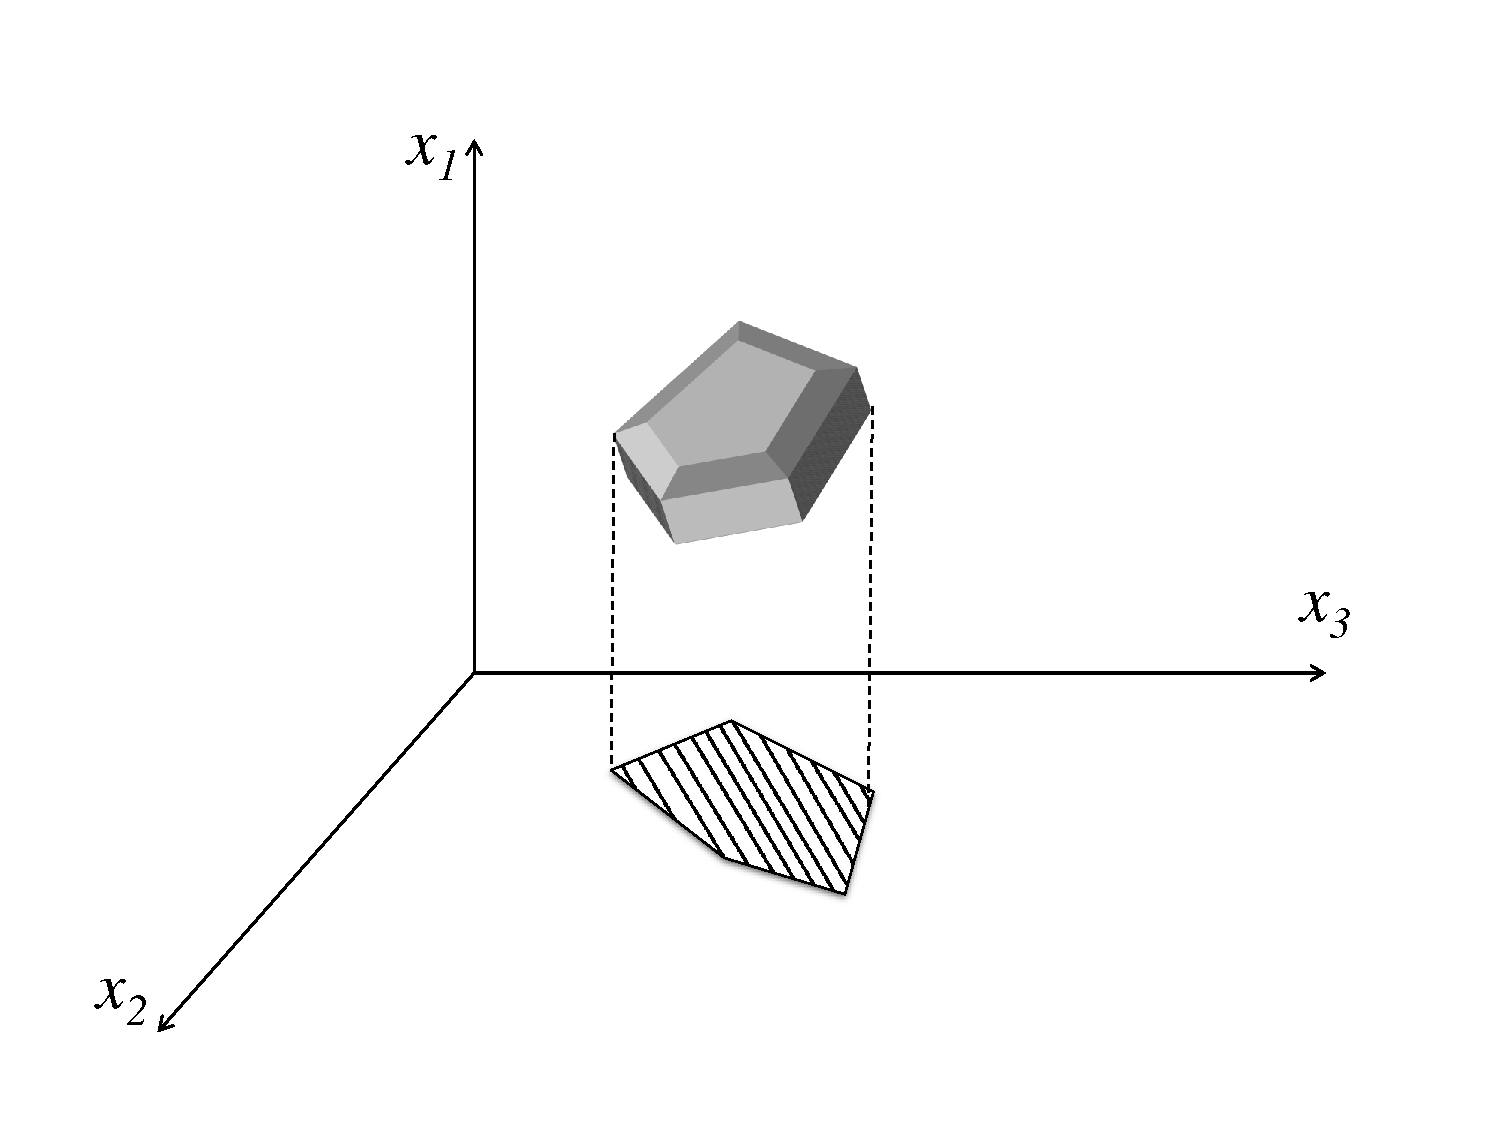
\includegraphics[width=\textwidth]{newfig/projection.pdf}
\caption{An example of projection from $\Fq^3$ to $\Fq^2$.}
\label{fig:3Dprojection}}
\end{figure}

Formally, we define concepts of the projection and elimination ideals:
\begin{Definition}
The {\bf $l$-th projection} mapping is defined as:
$$\pi_l:\Fq^d\to\Fq^{d-l},~~\pi_l((x_1,\dots,x_d)) = (x_{l+1}.\dots,x_d)$$
where $l<d$. For any subset $V \subseteq \Fq^d$, we write 
$$\pi_l(V) = \{\pi_i(x):x\in A\}\subseteq \Fq^{d-l}$$
\end{Definition}

\begin{Definition}
Let $J$ be an ideal in  $\Fq[x_1,\dots,x_d]$. The $l$-th 
{\bf elimination ideal} $J_l$ is the ideal of $\Fq[x_{l+1},\dots,x_d]$ defined
by
\begin{equation}
J_l = J \cap \Fq[x_{l+1},\dots,x_d]
\end{equation}
\end{Definition}

The elimination ideal $J_l$ has eliminated all the variables 
$x_1,\dots,x_l$, i.e., it only contains polynomials with variables in
$x_{l+1},\dots,x_d$. 
In a general setting,
$\pi_l(V_d(J))$ from $\Fq^d$ to $\Fq^{d-l}$ is a subset of $V(J_l)$. But over $\Fq$, 
consider ideal $J+J_0$ where $J_0$ is the ideal of vanishing polynomials, it is proved in \cite{gao:qe-gf-gb}
that 
$$\pi_l(V(J+J_0)) = V((J+J_0)_l).$$
This shows that in finite fields, projection of the variety $V_{d}(\langle f_1,\dots,f_s\rangle)$
from $\Fq^d$ to $\Fq^{d-l}$, is exactly the variety $V_{d-l}(\langle f_1,\dots,f_s\rangle\cap \Fq[x_{l+1},\dots,x_d])$.

Elimination theory uses {\bf elimination ordering} 
to systematically eliminate variables from a system of polynomial
equations.
We can generate elimination ideals by computing
\Grobner bases using elimination orderings. 

\begin{Theorem}[Elimination Theorem]
%$\left[\bf{Elimination\  Theorem}\right]$
Let $J$ be an ideal in $\F[x_1,\dots,x_d]$ and let $G$ be the \Grobner 
basis of $J$ with respect to the lex order (elimination order) 
$x_1>x_2>\dots>x_d$. Then, for every $0\leq l\leq d$,
\begin{equation}
G_l=G\cap \F[x_{l+1},\dots,x_d]
\end{equation}
is a \Grobner basis of the $l$-th elimination ideal $J_l$.
\label{thm:elimth}
\end{Theorem}

This can be better understood using the following example.

\begin{Example}
Given the following equations in $\R[x,y,z]$
\begin{eqnarray}
x^2+y+z&=1 \nonumber \\
x+y^2+z&=1 \nonumber \\
x+y+z^2&=1 \nonumber
\end{eqnarray}
let $I$ be the ideal generated by these equations:
\begin{equation}
I=\langle x^2+y+z-1, x+y^2+z-1, x+y+z^2-1\rangle \nonumber
\end{equation}
The \Grobner basis for $I$ with respect to lex order $x>y>z$ is 
found to be $G=\{g_1,g_2,g_3,g_4\}$ where
\begin{eqnarray}
g_1&=&x+y+z^2-1 \nonumber \\
g_2&=&y^2-y-z^2+z \nonumber \\
g_3&=&2yz^2+z^4-z^2 \nonumber \\
g_4&=&z^6-4z^4+4z^3-z^2 \nonumber
\end{eqnarray}

Notice that while $g_1$ has variables in $\R[x,y,z]$, $g_2$ and $g_3$ only 
have variables in $\R[y,z]$ and $g_4$ only has variables in $\R[z]$. Thus, 
$G_1=G\cap \R[y,z]=\{g_2,g_3,g_4\}$ and $G_2=G\cap \R[z]=\{g_4\}$

Also notice that since $g_4$ only contains variable $z$, and since $g_4=0$, 
a solution for $z$ can be obtained. This solution can then be applied to 
$g_2$ and $g_3$ to obtain solutions for $y$, and so on.
\end{Example}

Elimination theory provides the basis for the following abstraction approach.
\subsection{Abstraction Using Nullstellensatz and Gr\"obner Basis}
\begin{Problem}
\label{setup:abs}
Let $S$ be the system of polynomials, 
$\{f_1,\dots,f_s,f_{A_1},\dots,f_{A_n},f_{Z}\}\subset \Fkk$, 
derived from the hardware
implementation of any circuit over $\Fq, q=2^k$, as Figure \ref{fig:abs_setup} shows.
In general, this circuit performs some unknown function $f$ over 
$\Fq$ such that every $f:\Fq\to\Fq$ is represented in polynomial form.
For any circuit $\mathcal C$, $Z = \Func(A)$. Then how to derive this function $\Func$
using GB?
\end{Problem}

\begin{figure}[bp]
\centering{
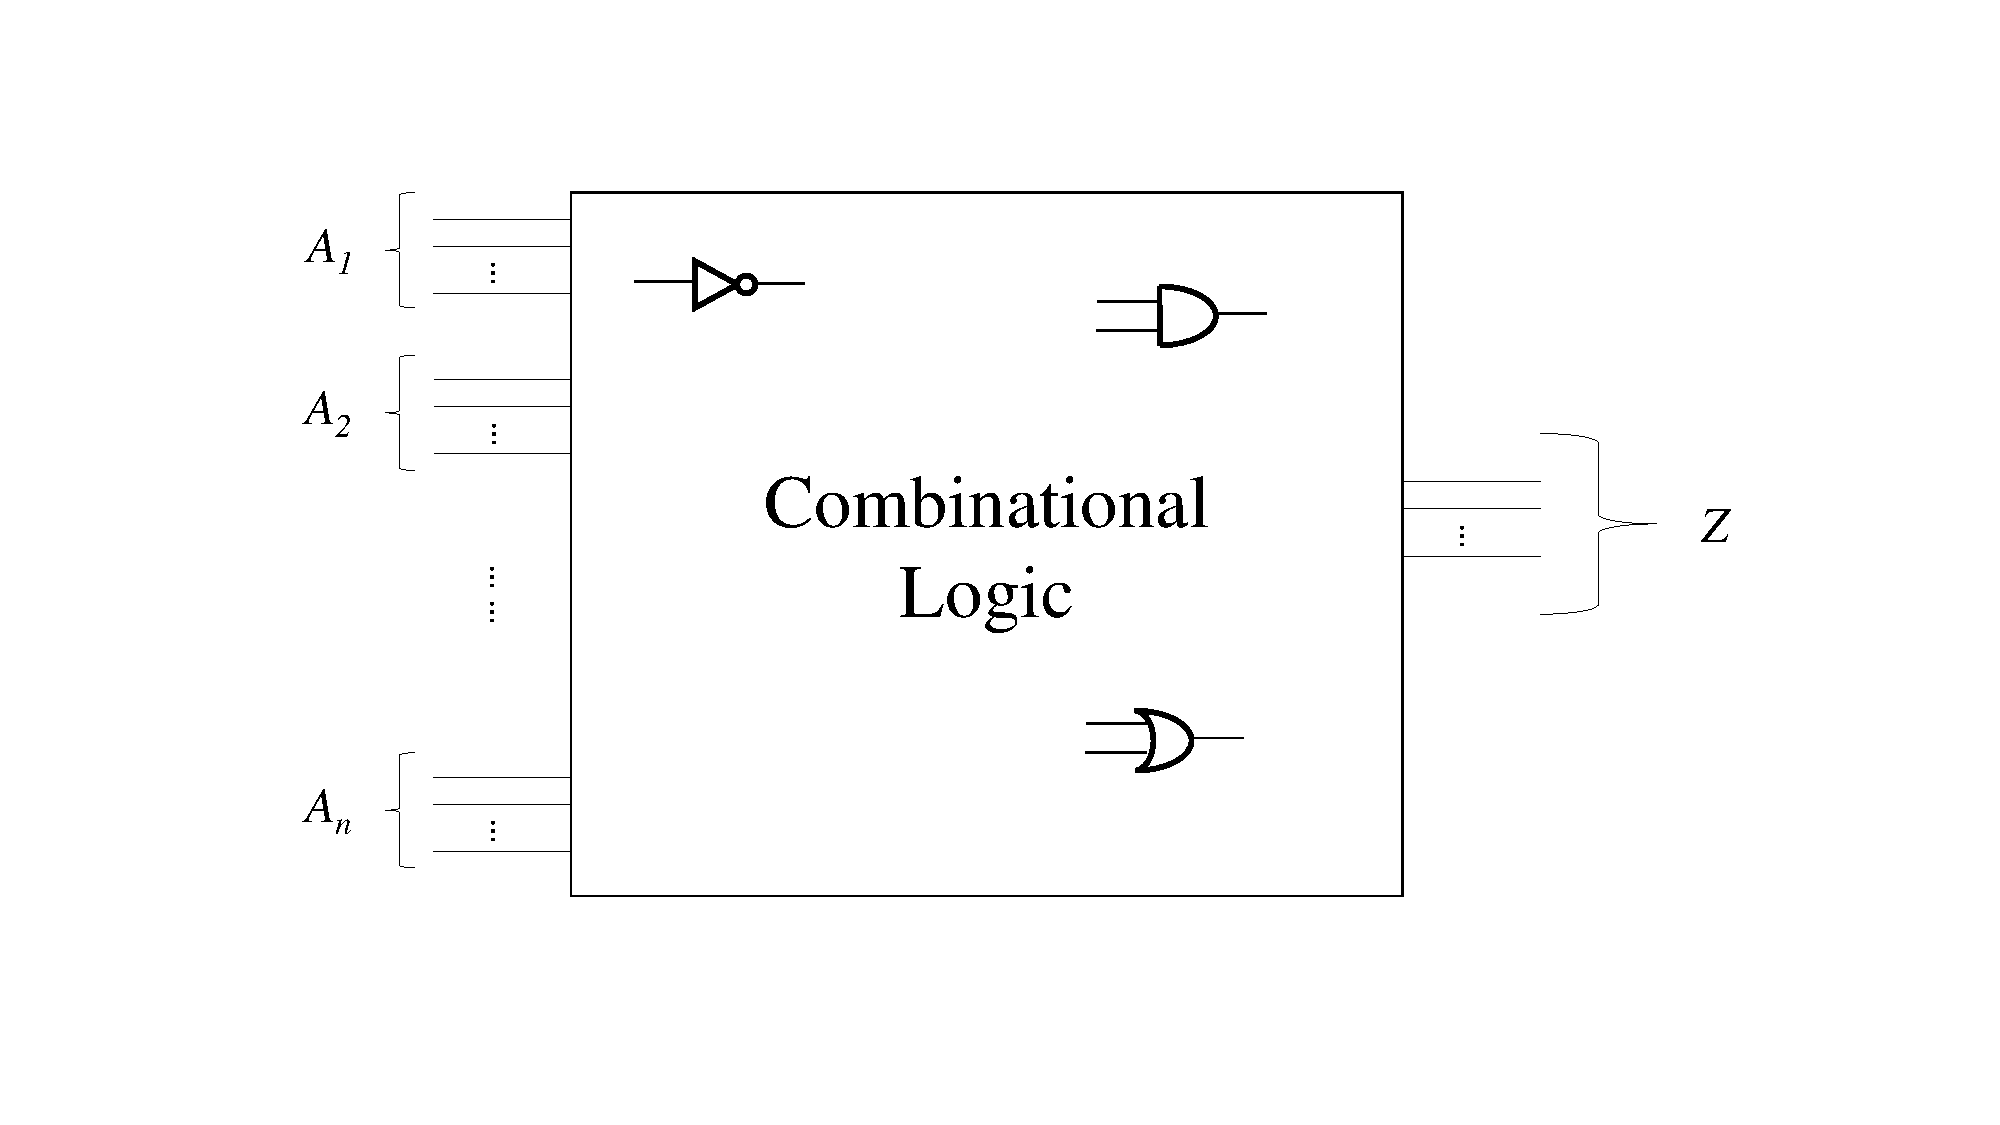
\includegraphics[width=\textwidth]{newfig/abs_setup.pdf}
\caption{Galois field arithmetic circuit model for abstraction.}
\label{fig:abs_setup}}
\end{figure}

The polynomial representation of $\Func$ over $\Fkk$ is:
\begin{equation}
f_{\Func}: Z+\Func(A_1,\dots,A_n) \nonumber
\end{equation}

Since $f_{\Func}$ is ultimately derived from the circuit implementation, 
it agrees with the solution to the system of polynomials $\{S\}=0$, i.e.,:
\begin{equation}
f_1=\dots=f_s=f_{A_1}=\dots=f_{A_n}=f_{Z}=0 \nonumber
\end{equation}
Thus, if we let $J=\langle f_1,\dots,f_s,f_{A_1},\dots,f_{A_n},f_{Z}\rangle$ 
be the ideal generated by $S$, 
$f_{\Func}$ {\bf vanishes} on the variety $V_{\Fkk}(J)$. 
Therefore, due to Proposition \ref{pro:iofv}, 
$f_{\Func}$ must be contained in the ideal of polynomials that vanish on
this variety, $f_{\Func} \in I(V_{\Fkk}(J))$. 

By applying Strong Nullstellensatz over $\Fkk$ (Theorem \ref{thm:sns}), 
$I(V_{\Fkk}(J))=J+J_0$ where
$J_0$ is the ideal generated by all vanishing polynomials in $\Fkk$. 
Recall that a vanishing polynomial in $\Fkk[x]$ is $x^q-x=x^q+x$. 
In our case, 
$\{x_1,\dots,x_d\} \in \F_2$ and $\{A_1,\dots,A_n,Z\} \in \Fkk$.
Thus, for $\Fkk[x_1,\dots,x_d,A_1,\dots,A_n,Z]$: 
\begin{equation}
J_0 = \langle x_1^2+x_1,\dots,x_d^2+x_d, A_1^{2^k}+A_1,\dots,A_n^{2^k}+A_n,Z^{2^k}+Z\rangle \nonumber
\end{equation}

The generators of the ideal sum $J+J_0$ are simply the combination of the 
generators of $J$ and the generators $J_0$.



The variety $V_{\Fq}(J)$ is
the set of all consistent assignments to the nets (signals) in the
circuit $C$. If we {\it project this variety on the word-level input and
output variables of the circuit $C$, we essentially generate the
function $\Func$ implemented by the circuit.} Projection of varieties from
$d$-dimensional space $\Fq^d$ onto a lower dimensional subspace
$\Fq^{d-l}$ is equivalent to {\it eliminating $l$ variables} from the
corresponding ideal. This can be done by computing a \Grobner basis
of the ideal with elimination ordering, as described in the 
Elimination Theorem (Theorem \ref{thm:elimth}).
Thus, we can find the polynomial 
$f_\Func:Z+\Func(A_1,\dots,A_n)$ by computing the \Grobner
basis of $J+J_0$ using the proper elimination ordering.

The proposed elimination order for 
abstraction is defined as the {\bf abstraction term order}. 
\begin{Definition}
\label{def:ato}
Given a circuit $C$,
let $x_1, \dots, x_d$ denote all the bit-level variables, 
let $A_1,\dots,A_n$ denote the $k$-bit word-level inputs, 
and let $Z$ denote the $k$-bit word-level output. 
Using any refinement of the partial variable order 
$\{x_1, \dots, x_d\} > Z > \{A_1, \dots, A_n\}$,
% where any refinement of the order will do,
impose a lex term order $>$ on the polynomial ring 
$R = \Fq[x_1, \dots, x_d, Z, A_1, \dots, A_n]$. 
This elimination term order $>$ is defined as
the {\bf Abstraction Term Order (ATO)}. The relative ordering among $x_1,
\dots, x_d$ is not important and can be chosen arbitrarily. Likewise,
the relative ordering among $A_1, \dots, A_n$ is also unimportant.
\end{Definition}

\begin{Theorem}[Abstraction Theorem \cite{tim:phd}]
Using the notations from Problem Setup \ref{setup:abs} at the beginning of this subsection,
we compute a \Grobner basis $G$ of ideal $(J+J_0)$ using the abstraction term 
order $>$. Then: \\
1) For every word-level input $A_i$, $G$ must contain the vanishing 
polynomial $A_i^q - A_i$ as the only polynomial with $A_i$ as its only 
variable;\\
2) $G$ must contain a polynomial of the form 
$Z + \mathcal{G}(A_1,\dots,A_n)$; and\\ 
3) $Z + \mathcal{G}(A_1,\dots,A_n)$ is such that 
$\Func(A_1,\dots,A_n) = {\mathcal{G}}(A_1,\dots,A_n),
\forall A_1,\dots,A_n \in \Fq$. 
In other words, ${\mathcal{G}}(A_1,\dots,A_n)$ and $\Func(A_1,\dots,A_n)$ are
equal as polynomial functions over $\Fq$.
\label{thm:abs}
\end{Theorem}

\begin{Corollary}
By computing a {\bf reduced} \Grobner basis $G_r$ of $J + J_0$, 
$G_r$ will contain one and only one polynomial in of the form 
$Z + \G(A_1,\dots,A_n)$, such that $Z = \G(A_1,\dots,A_n)$ is the 
{\bf unique, minimal, canonical} representation of the function 
$\Func$ implemented by the circuit.  
\end{Corollary}

\begin{Example}
\label{exp:finalMul2Bit}
Consider a 2-bit multiplier over ${\mathbb{F}}_{2^2}$ with
$P(x)=x^{2}+x+1$, given in Figure \ref{fig:2bitmul}. Variables $a_0,
a_1, b_0, b_1$ are primary inputs, $z_0, z_1$ are primary outputs, and
$c_0, c_1, c_2, c_3, r_0$ are intermediate variables. 
%The gate $\otimes$
%corresponds to AND-gate, i.e. bit-level multiplication modulo 2. The
%gate $\oplus$ corresponds to XOR-gate, i.e. addition modulo 2.

\begin{figure}[bp]
\centerline{
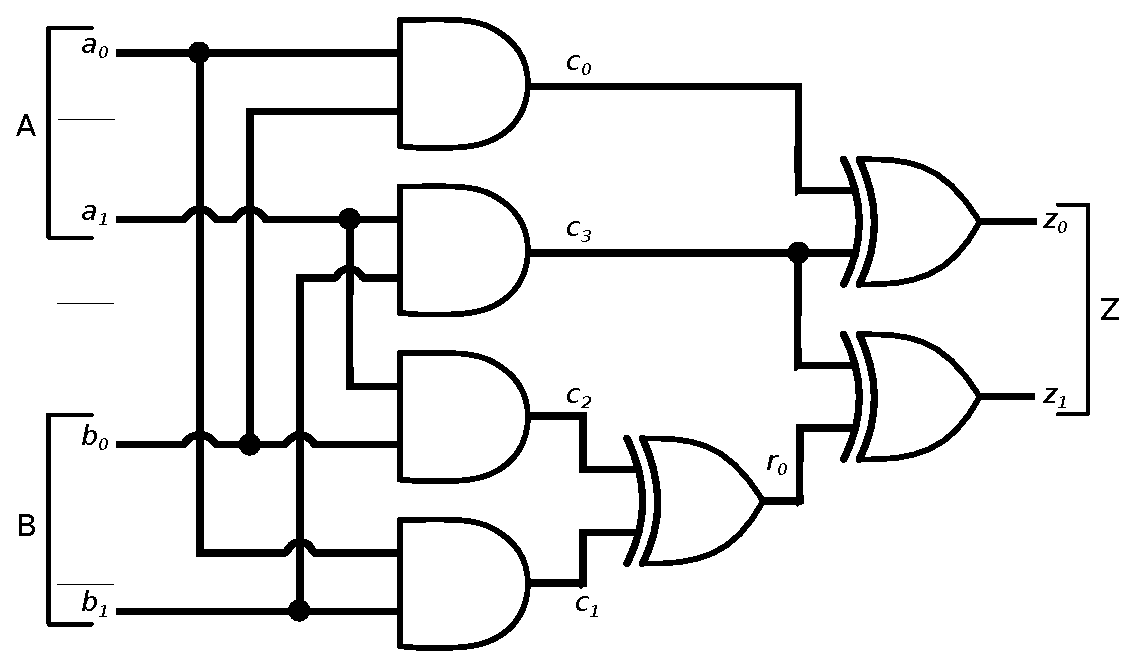
\includegraphics[scale=0.5]{./figures/2bitmasmult.eps}
}
\caption{ A 2-bit multiplier over ${\mathbb{F}}_{2^2}$.}
\label{fig:2bitmul}
\end{figure}

Polynomials extracted from the circuit implementation represent the
ideal $J$. Along with the ideal of vanishing polynomials $J_0$, 
the following polynomials represent the generators 
of $J+J_0$ for the multiplier circuit. 

\begin{eqnarray}
 \left .  
	\begin{aligned}
		f_1:c_0+a_0 \cdot b_0  \\
		f_2:c_1+a_0 \cdot b_1  \\
		f_3:c_2+a_1 \cdot b_0  \\
		f_4:c_3+a_1 \cdot b_1  \\
		f_5:r_0+c_1 + c_2		\\
		f_6:z_0+c_0 + c_3		\\
		f_7:z_1+r_0 + c_3		
	\end{aligned} 
 \ \right\}
 &\qquad&  {\it  \text{Bit-level circuit constraints} ~(\subset J)} \nonumber \\
 \left . 
	\begin{aligned}
		f_{A}:A+a_0+a_1\cdot \alpha   \\ 
		f_{B}:B+b_0+b_1\cdot \alpha  \\ 
		f_{Z}:Z+z_0+z_1\cdot \alpha   
	\end{aligned} 
 \right\}
 &\qquad&  {\it  \text{Word-level designation} ~(\subset J)} \nonumber \\
  \left . 
	\begin{aligned}
		a_0^2-a_0, ~a_1^2-a_1,~b_0^2-b_0, ~b_1^2-b_1   \\ 
		c_0^2-c_0, ~c_1^2-c_1,~c_2^2-c_2, ~c_3^2-c_3  \\ 
		r_0^2-r_0, ~z_0^2-z_0,~z_1^2-z_1    \\ 
		A^4-A, ~B^4-B ,~Z^4-Z		  
	\end{aligned} 
 \right\}
 &\qquad&  {\it \text{vanishing polynomials} (J_0)} \nonumber
\end{eqnarray}
We apply abstraction term order $>$, i.e a lex order with
"bit-level variables" $>$ "Output Z" $>$ "Inputs A, B".

When we compute the reduced \Grobner basis, $G_r$, of \{$J + J_0$\} with 
respect to this ordering, $G_r$ = \{$g_1, \dots, g_{14}\}:$
\begin{align*}
&g_1: B^4+B; 
~~g_2: b_0+b_1 \alpha + B; 
~~g_3: a_0+a_1 \alpha + A;  \nonumber \\
&g_4: c_0+c_1 \alpha + c_2 \alpha + c_3(\alpha+1)+Z;
g_5: r_0+c_1+c_2; 
~~g_6: z_0+c_0+c_3; \nonumber \\
&g_7: z_1+r_0+c_3; 
~~{\bf g_8: Z+A\cdot B};
~~g_9: b_1+B^2+B; 
~~g_{10}: a_1+A^2+A; \nonumber \\
&g_{11}: c_3+a_1\cdot b_1
g_{12}: c_2+a_1\cdot b_1 \alpha + a_1 \cdot B; 
~~g_{13}: c_1+a_1\cdot b_1 \alpha +b_1 A; 
~~g_{14}: A^4+A  \nonumber
\end{align*}

Here $g_8=Z+A\cdot B$ is the {\bf canonical, word-level polynomial } 
representing the function performed by the multiplier $Z=A\cdot B$.
\end{Example}

\section{Concluding Remarks}
Our approach to word-level abstraction of Galois field arithmetic 
circuits applies concepts of polynomial ideals, varieties, \Grobner basis, 
and abstraction theory to implement verifications on sequential circuits. 
The application of these approaches to sequential circuit verification is described in the following chapters. 

\chapter{Word-Level Traversal of Finite State Machines using Algebraic Geometry}
\label{ch:reacha}
Reachability analysis is a basic component of sequential circuit verification, especially for 
formal equivalence checking and model checking techniques. Concretely, in modern synthesis 
tools, in order to improve various performance indicators such as latency, clock skew or power
density, sequential optimization techniques such as retiming \cite{retiming}, scan logic \cite{scan},
sequential power optimization \cite{mathur2009power} and clock-gating techniques \cite{clockgating} are applied.
% some major refactoring and attachments are made on original designs. 
These modifications may introduce bugs, errors or malfunctions to the original logic and cause problems. 
Based on traditional localized simulation or formal verification method ({\it e.g.} equivalence checking), 
designers are reluctant to make aggressive optimization
since the malfunctions are considered as ``faults" in the circuits.
However, if the circuit behavior is carefully investigated, it may become evident that 
those ``faults" may never be activated during a restricted execution starting 
from legal initial states and with legal inputs. Thus we will call those ``faults" as 
{\it spurious faults} (false negatives), since they will not affect the circuit's normal behavior.

Almost all practical sequential logic components can be modeled as finite state machines (FSMs). 
If we apply constraints upon the machine to make it start from designated initial states, and 
take specific legal inputs, a set of reachable states can be derived. 
As long as the ``faults" can be modeled as ``bad states", we can judge whether they are 
spurious faults by checking if they belong to the unreachable states. From the spurious fault validation 
perspective, reachability analysis is a must when developing full set of sequential circuit verification
techniques.

There are quite a few methods to perform reachability checking on FSMs. One among them is 
state space traversal. Conventionally, the algorithm is based on bit-level techniques such as
binary decision diagrams (BDDs) and Boolean logic. We propose a new traversal algorithm on word-level,
which brings critical advantages. In this chapter the approach will be described and discussed in depth, 
with examples and experiments showing its feasibility when applied on general circuit benchmarks.

\section{Motivation}
Before introducing the details of our approach, there are a few questions to ask: what is 
the benefit of executing FSM traversal at word-level? How can algebraic geometry make this happen?
The answers can be found in this section, as a statement of the motivation of our research.

\subsection{FSM Traversal Algorithms}
Sequential circuits are modeled as FSMs, which can be implemented as graphs. Thus a 
graph-traversal based algorithm is created to analyze the reachable states \cite{coudert2003unified}.
A traversal algorithm using the concept of implicit state enumeration is proposed \cite{cho1993redundancy}.
Concretely, the algorithm is given in Algorithm \ref{alg:BFS}:

% \begin{algorithm}[H]
% \SetAlgoNoLine
% \LinesNumbered
%  \KwIn{Sequential circuit with given number of registers}
%  \KwOut{Scan registers listed in decreasing order of their non-controllability}
% 
%   $from^0 = reached = S^0$\;
%   $i = 0$\;
%   \While{TRUE}
%   {
%   	$i++$\;
% 	$to^i = $IMAGE$(\Delta,from^{i-1})$\;
% 	$new^i = to^i \cdot \overline{reached}$\;
% 	\For{each state variable $r_j$}
% 	{
% 		record\_if\_transitions\_present\_or\_missing$(r_j,new^i)$\;
% 		compute\_degree\_of\_unsettability$(r_j,new^i)$\;
% 	}
% 	\If{$new^i == 0$}
% 	{
% 		break\;
% 	}
% 	$reached = reached + new^i$\;
% 	$from^i = new^i$\;
%   }\
% \Return{$reached$}
% \caption {FSM Traversal using Implicit State Enumeration\cite{KallaPartialScan}}
% \label{alg:SIMPSON}
% \end{algorithm}
% \DecMargin{1em}

% \IncMargin{1em}
\begin{algorithm}[hbt]
\SetAlgoNoLine
\LinesNumbered
% \Indm
 \KwIn{Transition functions $\Delta$, initial state $S^0$}
% \Indp

  $from^0 = reached = S^0$\;
  \Repeat{$new^i == 0$}
  {
  	$i \gets i + 1$\;
	$to^i \gets$Img$(\Delta, from^{i-1})$\;
	$new^i \gets to^i \cap \overline{reached}$\;
  	$reached \gets reached \cup new^i$\;
	$from^i \gets new^i$\;
  }
\Return{$reached$}
\caption {BFS Traversal for FSM Reachability}\label{alg:BFS}
\end{algorithm}
% \DecMargin{1em}

Above algorithm describes a breath-first-search (BFS) traversal in
state space. The traversal algorithm is a simple variation of BFS algorithm where 
states are nodes and transitions are arcs. Each state is uniquely encoded by a combination
of a set of register data, which is usually represented by a Boolean vector. 

Since a typical sequential circuit usually contains a combinational logic
component, the traversal algorithm analyzes the combinational logic and derives the transition 
function for one-step reachability within current time-frame, and extends the result to complete 
execution paths through unrolling. If each state encoding ({\it i.e.} exact values in the selected registers) is
explicitly analyzed and counted during the unrolling 
procedure, this unrolling is called {\bf explicit unrolling}. In the BFS traversal algorithm, the states cannot be 
directly read in the execution; instead, they are implicitly represented using a conjunction of several 
Boolean formulas. Such techniques differs from explicit unrolling are called {\bf implicit unrolling}.

However, the BFS traversal algorithm proposed by the author is usually not practical. The conjunctions of 
Boolean formulas are stored as BDDs, which is a canonical and convenient structure. Nevertheless, 
the size of BDD explodes when the formulas become too long and too complicated. In \cite{cho1993redundancy},
the authors make a compromise between accuracy and cost, and turn to approximate reachability. 
In this research work, the aim is to explore a word-level technique which can make a accurate reachability
analysis available.

\subsection{Word-Level Data Flow on Modern Datapath Designs}
The level of integration of modern digital circuit designs is very high. For example, processor A10 designed by Apple
integrates 3.3 billion transistors on a $125~mm^2$ chip \cite{AppleA10}. Such a high density makes the silicon 
implementation of large datapaths possible. In recent decades, 64-bit or even larger datapaths frequently appear in 
modern digital IC designs such as powerful central processing units (CPUs) and high bandwidth memory (HBM).
Meanwhile, with the development of electronic design automation (EDA) tools, data flow 
is described by the designer as word-level specifications. Therefore, it will be straightforward 
and beneficial for users if formal verification tools can work on word-level. Moreover, adopting word-level 
techniques will greatly reduce the state space and make verification more efficient.

In order to throw light on the advantages using word-level techniques, we pick a typical 
digital circuit component in modern 64-bit MIPS processor as an example.

\begin{Example}
Figure \ref{fig:MIPS} depicts a sequential multiplication hardware implementation within a 64-bit 
MIPS. Initially, one multiplicand is preloaded to the lower 64 bits of the product registers. 
Iteratively, the last significant bit (LSB) of current (temporary) product is used as flag to activate the ALU 
to add on the other multiplicand. For each iteration the data in product registers shifts right by 1 bit.
Finally when the most significant bit (MSB) of preloaded multiplicand arrives at the MSB of product registers,
the registers contains the result -- 128 bits product. The behavior can be described by the following algorithm:

% \vspace{0.2in}

% \IncMargin{1em}
\begin{algorithm}[H]
\SetAlgoNoLine
\LinesNumbered
% \Indm
 \KwIn{Multiplicand $A,B$}
 \KwOut{Product $C$}
% \Indp

  Preload $B$ into lower 64-bit of Product Register $P$\;
  \Repeat{64 Repetitions}
  {
  	\If{Last Bit of Product Register $LSB(P)==1$}
  	{
		$P = P_{1/2}+B$\;
	}
	Right shift $P$\;
  }
\Return{$C=P$}
\caption {Sequential multiplication hardware in 64-bit MIPS}\label{alg:MIPS}
\end{algorithm}
% \DecMargin{1em}

\begin{figure}[bp]
\centering{
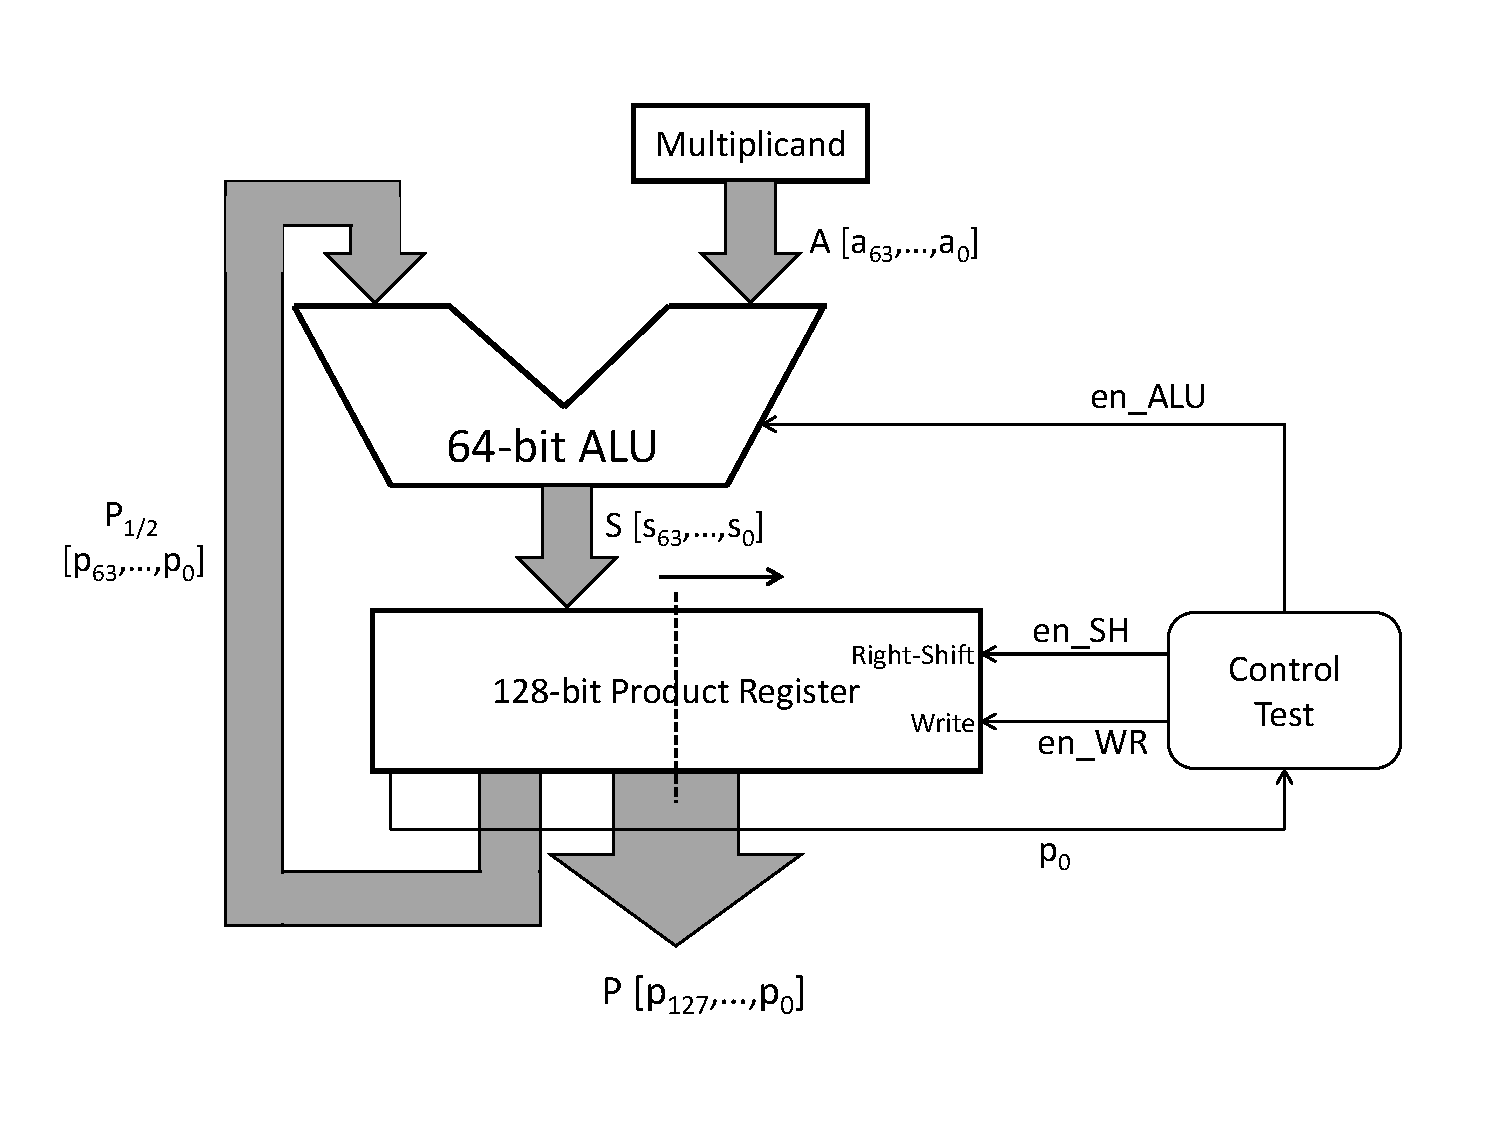
\includegraphics[width=\textwidth]{newfig/MIPS.pdf}
\caption{A 64-bit sequential multiplication hardware design.}
\label{fig:MIPS}}
\end{figure}

% List the detailed bit-level property need to check P==P+B
Traditionally, to verify the functional correctness of this multiplier, satisfiability (SAT) based or BDD based 
model checking is applied on basic function units. For example, as a part of functional verification, 
we would like to check ``$P=P_{1/2}+B$" is correctly executed. Then in a model checker we need to add following 
specifications:

\begin{align*}
& en\_ALU \\
\land & s_0 = a_0 \oplus p_0 \\
\land & s_1 = a_1 \oplus p_1 \oplus (a_0 \land p_0) \\
\land & s_2 = a_2 \oplus p_2 \oplus ((a_1 \oplus p_1) \land a_0 \land p_0 \lor a_0 \land p_0) \\
\land & \cdots \\
\land & s_{63} = a_{63} \oplus p_{63} \oplus (c_{63})
\end{align*}

We can see that when checking a single part of the whole structure, the number of clauses 
needed will increase to $k+1$ when using $k$-bit datapath. Considering the formula representing 
carry-in will become longer and longer, the final conjunction of all clauses will contain 
$O(2^k)$ Boolean operators. If by some means we can write the specification with only 3 variables:
\begin{equation}
\label{eqn:wordspec}
S=P_{1/2}+B
\end{equation}

The abstraction to word-level will reduce symbolic storage and execution cost; the complexity 
to traverse the state space will be greatly reduced.
\end{Example}

On the other hand, when implementation details of the datapath are not available, it is not convenient 
any more for users of conventional model checker. The reason is that the user has to write all clauses 
for the implementation, which contains cross-literals, {\it e.g.} $s_2$ may associate with $a_1, p_0$, {\it etc.} If the user 
is not familiar with the implementation of this adder, those cross-literals will bring
confusions. However, if word-level techniques allow specification like Equation \ref{eqn:wordspec},
the verification tool will be very user-friendly and straightforward even if the implementation details
are in a black box.

\subsection{On the Existence of Word-Level Abstraction for Arbitrary Circuits}
When given a bit-level netlist, the prerequisites to use word-level techniques are to convert bit-level 
to word-level first. This conversion is usually completed by abstraction techniques.

An old but universally effective abstraction method is {\it Lagrange's interpolation}, 
which can be applied over finite fields. Here we use an example to illustrate the 
conversion in Galois field using Lagrange's interpolation for an arbitrary circuit.

\begin{Example}[Lagrange's interpolation]
Assume we are given gate-level netlist shown in Figure \ref{fig:Lagrange}. It can be written as 3 
Boolean equations:
\begin{align*}
z_0 &= a_0 \lor a_1 \lor a_2 \\
z_1 &= a_1 \land \neg a_2 \lor a_0 \land \neg a_1 \land a_2 \\
z_2 &= a_1 \lor \neg a_0 \land a_2
\end{align*}
Define 2 word-level variables $A,Z$ as input and output:
$$A = \{a_2a_1a_0\},~Z = \{z_2z_1z_0\}$$
To convert bit-level to word-level, we need to find mapping $\mathbb{B}^3 \rightarrow \mathbb{B}^3$,
or $\F_{2^3} \rightarrow \F_{2^3}$. The latter one, as mentioned in preliminaries, is a polynomial
function in $\F_{2^3}$.

\begin{figure}[bp]
\centering{
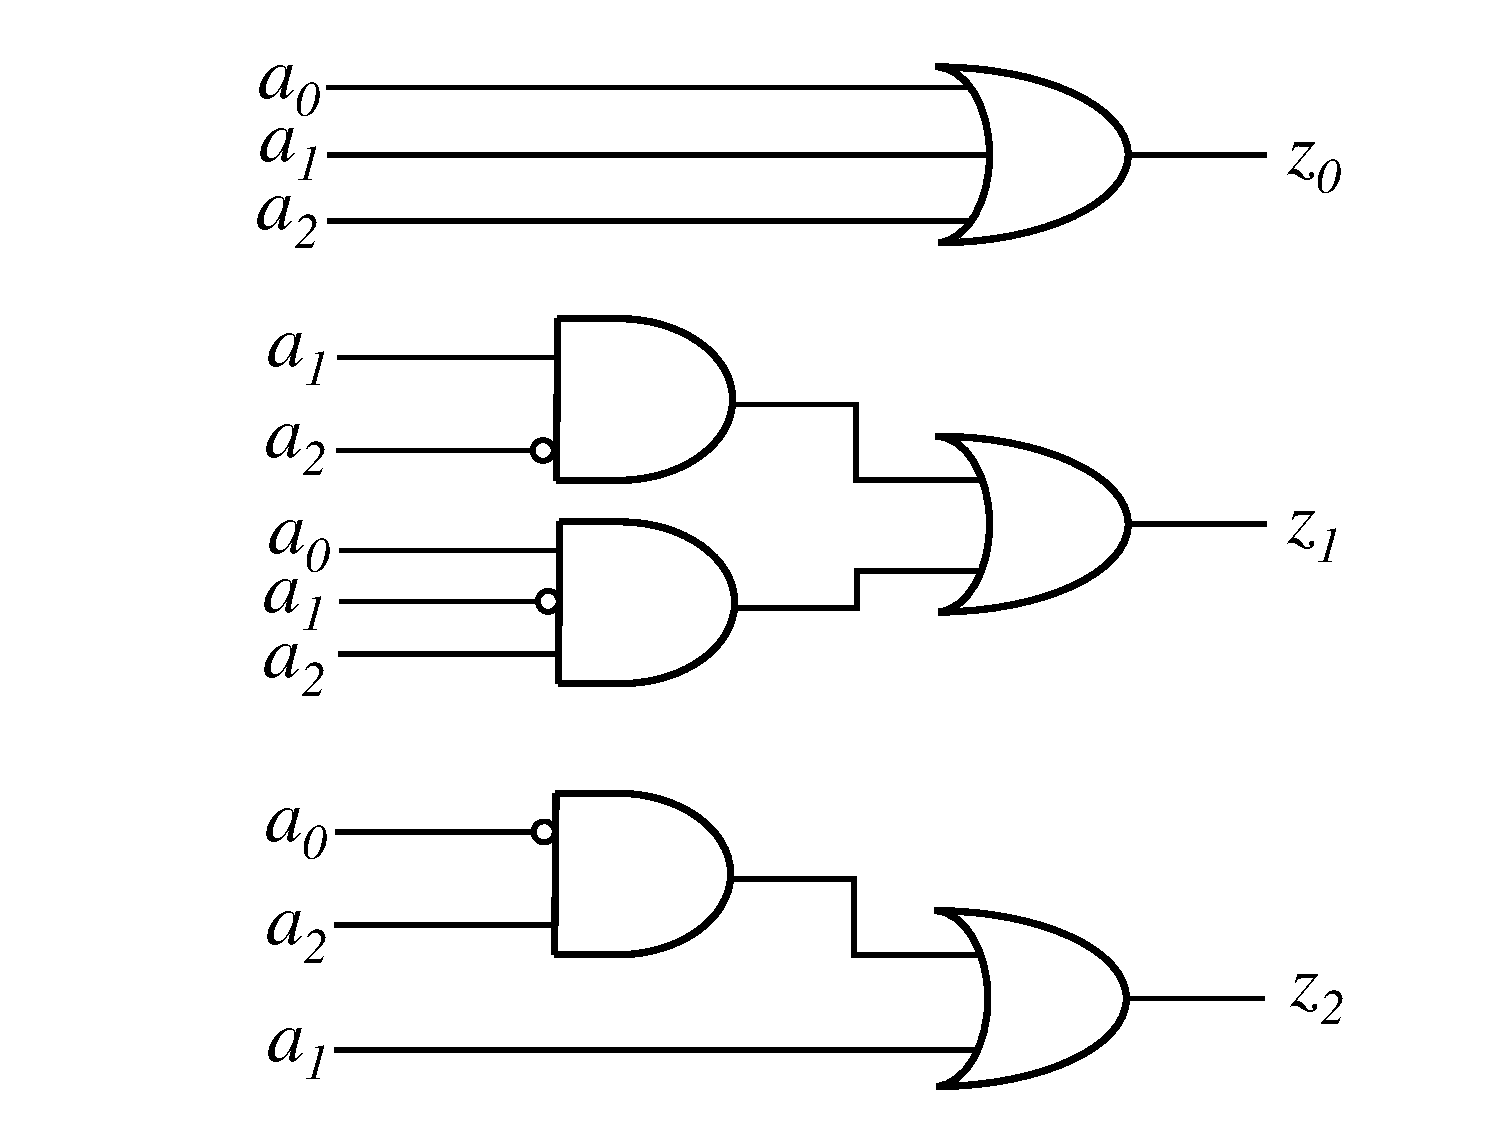
\includegraphics[width=4in]{newfig/Lagrange.pdf}
\caption{Gate-level netlist for Lagrange's interpolation example.}
\label{fig:Lagrange}}
\end{figure}

For each element in $\F_{2^3}$, we write down the truth table as Table \ref{tab:truthtable}.
Now our objective is to abstract a function over finite field $\F_{2^3}$ in word-level variables, {\it i.e.} 
$Z = \Func(A)$. Recall Lagrange's interpolation formula:
\begin{equation}
\label{eqn:Lagrange}
\Func(x) =  \sum_{k=1}^N \left[ \prod_{(0\leq j \leq k-1),(j\neq i)}\frac{x-x_j}{x_i-x_j} \cdot y_k \right]
\end{equation}

\begin{table}[bp]
\caption{Truth table for mappings in $\mathbb{B}^3$ and $\F_{2^3}$.}
\label{tab:truthtable}
\centering{\small
\begin{tabular}{|c|ccc|c|}
\hline
$\{a_2a_1a_0\}\in\mathbb{B}^3$   & $A\in \F_{2^3}$ &$\rightarrow$& $\{z_2z_1z_0\}\in\mathbb{B}^3$  & $Z\in \F_{2^3}$ \\
\hline
000  &0 &$\rightarrow$&000 & 0 \\
001  &1 &$\rightarrow$&001 & 1 \\
010  &$\alpha$ & $\rightarrow$ & 111& $\alpha^2 + \alpha + 1$ \\
011  &$\alpha + 1$ &$\rightarrow$& 111 & $\alpha^2 + \alpha + 1$ \\
100  &$\alpha^2$ &$\rightarrow$& 101 &  $\alpha^2+1$ \\
101  &$\alpha^2 + 1$ &$\rightarrow$&011 & $\alpha+1$ \\
110  &$\alpha^2 + \alpha$&$\rightarrow$& 101 &$\alpha^2 + 1$ \\
111  &$\alpha^2 + \alpha + 1$ &$\rightarrow$& 101 &$\alpha^2 + 1$\\
\hline
\end {tabular}
}
\end{table}

The geometric meaning of Lagrange's interpolation in real algebra is: given $N$ points with coordinates $(x_i,y_i)$,
they can always be fitted into a polynomial function with at most $N-1$ degree, and that function can be 
written in the form of Equation \ref{eqn:Lagrange}. In this example, although defined in a Galois field instead of 
the real number field, the essential concept of Lagrange's interpolation remains the same. 
We can get 8 points in the affine space:
\begin{align*}
\text{Generic form}&: (a_2\alpha^2+a_1\alpha+a_0,z_2\alpha^2+z_1\alpha+z_0) \gets (A,Z) \\
\text{Point }1&: (0, 0) \gets (000,000) \\
\text{Point }2&: (1,1) \gets (001,001) \\
\text{Point }3&:  (\alpha,\alpha^2 + \alpha + 1) \gets (010,111)\\
\text{Point }4&:  (\alpha + 1,\alpha^2 + \alpha + 1)\gets (011,111) \\
\text{Point }5&:  (\alpha^2,\alpha^2+1) \gets (100,101)\\
\text{Point }6&:  (\alpha^2 + 1,\alpha+1)\gets (101,011)\\
\text{Point }7&:  (\alpha^2 + \alpha,\alpha^2 + 1)\gets (110,101)\\
\text{Point }8&:  (\alpha^2 + \alpha + 1,\alpha^2 + 1)\gets (111,101)
\end{align*}
Substitute 8 $(x_i,y_i)$ pairs in Equation \ref{eqn:Lagrange} with these 8 points in $\F_{2^3}$.
The result is a polynomial function with degree no greater than 7:
\begin{align*}
Z =& \Func(A) \\
=& (\alpha^2+\alpha+1) A^7 + (\alpha^2+1) A^6 + \alpha A^5 + (\alpha+1) A^4 \\
&+ (\alpha^2+\alpha+1)A^3+ (\alpha^2+1)A
\end{align*}

\end{Example}

The Lagrange's interpolation theorem also proves the existence of a word-level abstraction for a bit-level netlist.
In practice, Lagrange's interpolation is not scalable. 
The reason is that it needs the entire function (state space), but usually we only have the circuit representation
of the FSM. Considering this fact, a symbolic method is needed.
Our approach in this section uses abstraction based on 
Gr\"obner basis with abstraction term order (ATO), which is briefly introduced in Section \ref{sec:abstraction}.

\subsection{Significance of Developing Word-Level Reachability Analysis}
% At the end of this section, we summarize each subsection and conclude the motivation of our research.
% First, we start from the basic FSM traversal algorithms and exhibit their
% difficulties to overcome. Secondly, we state the observation that word-level description is 
% increasingly important and common in characterizing the data flow on modern large-size datapaths. 
% Last but not least, we give instances that some prerequisites for supporting word-level techniques 
% are already available. 

Based on the aforementioned discussions, the importance of performing FSM traversal at word-level 
can bring a dimension of abstraction in sequential circuit reachability analysis.
To overcome the cost incurred by searching in a large space, we propose to use word-level 
polynomials to represent the states and transition relations. As a result, states are categorized into 
sets represented by a small number of word-level polynomials (more specifically, the varieties to the polynomial ideals),
and multiple transition relations are therefore merged together. All of these efforts reduce the cost of 
state space, meanwhile lowering the time complexity to traverse such a state space. As Lagrange's interpolation
confirms the existence of word-level abstraction for bit-level circuits, the concept
can be extended to encode the state space of sequential circuit by word-level polynomials in $\Fkk$.
% we prove the feasibility of word-level techniques on general circuits' verification.
% Thus we cover both the necessity and sufficiency of developing such 
% a word-level traversal technique in our work.
% They are also answers to the questions at the beginning of this section.

\section{FSM Reachability using Algebraic Geometry}
\label{sec:reach}
% \subsection{An example illustrating our proposed approach}
We use symbolic state reachability with algebraic
geometry concepts. It is an abstraction based on word operand
definition of datapaths in circuits, and it can be applied
to arbitrary FSMs by bundling a set of bit-level variables together as
one or several word-level variables.  The abstraction polynomial,
encoding the reachable state space of the FSM, is obtained through
computing a GB over $\Fkk$ of the polynomials of the circuit using an
elimination term order based on Theorem \ref{thm:elimth}.  

\subsection{FSM Model for Sequential Circuits}
A finite state machine (FSM) is a mathematical model of computation for designing and analyzing sequential logic 
circuits. If a FSM's primary outputs depend on primary inputs and present state inputs, it is named as a \textit{Mealy machine};
the formal definition is as follows:
\begin{Definition}
A Mealy machine is an $n$-tuple $\mathcal M = (\Sigma,O,S,S^0,\Delta,\Lambda)$ where
\begin{itemize}
\item $\Sigma$ is the input label, $O$ is the output label;
\item $S$ is the set of states, $S^0\subseteq S$ is the set of initial states;
\item $\Delta:\ S\times\Sigma\to S$ is the next state transition function;
\item $\Lambda:\ S\times\Sigma\to O$ is the output function.
\end{itemize}
\end{Definition}
The other kind of FSM is \textit{Moore machine}, its difference from Mealy machine is that
its primary outputs only depend on the present states, {\it i.e.} the output function is defined as
$$\Lambda:\ S \to O$$
Typical sequential circuits can be depicted as Figure \ref{fig:seqmodel}(a). Primary inputs
$x_1,\dots,x_m \in \Sigma$, and primary outputs $z_1,\dots,z_n\in O$. Signals $s_1,\dots,s_k$ 
are present state (PS) variables, $t_1,\dots,t_k$ are next state (NS) variables.
We can define 2 $k$-bit words denoting the PS/NS variables as there are $k$ flip-flops
in the datapath: $S = (s_1,\dots,s_k), ~T=(t_1,\dots,t_k)$. Transition function
at bit level are defined as $\Delta_i$: 
$$t_i = \Delta_i(s_1,\dots,s_k,x_1,\dots,x_m)$$

In some cases, arithmetic computations are implemented as Moore machines where input operands
are loaded into register files $R$ and the FSM is executed for $k$ clock cycles.
We can simplify them to the model in Figure \ref{fig:seqmodel}(b).

\begin{figure}[bp]
\centering{
%\begin{minipage}{12cm}
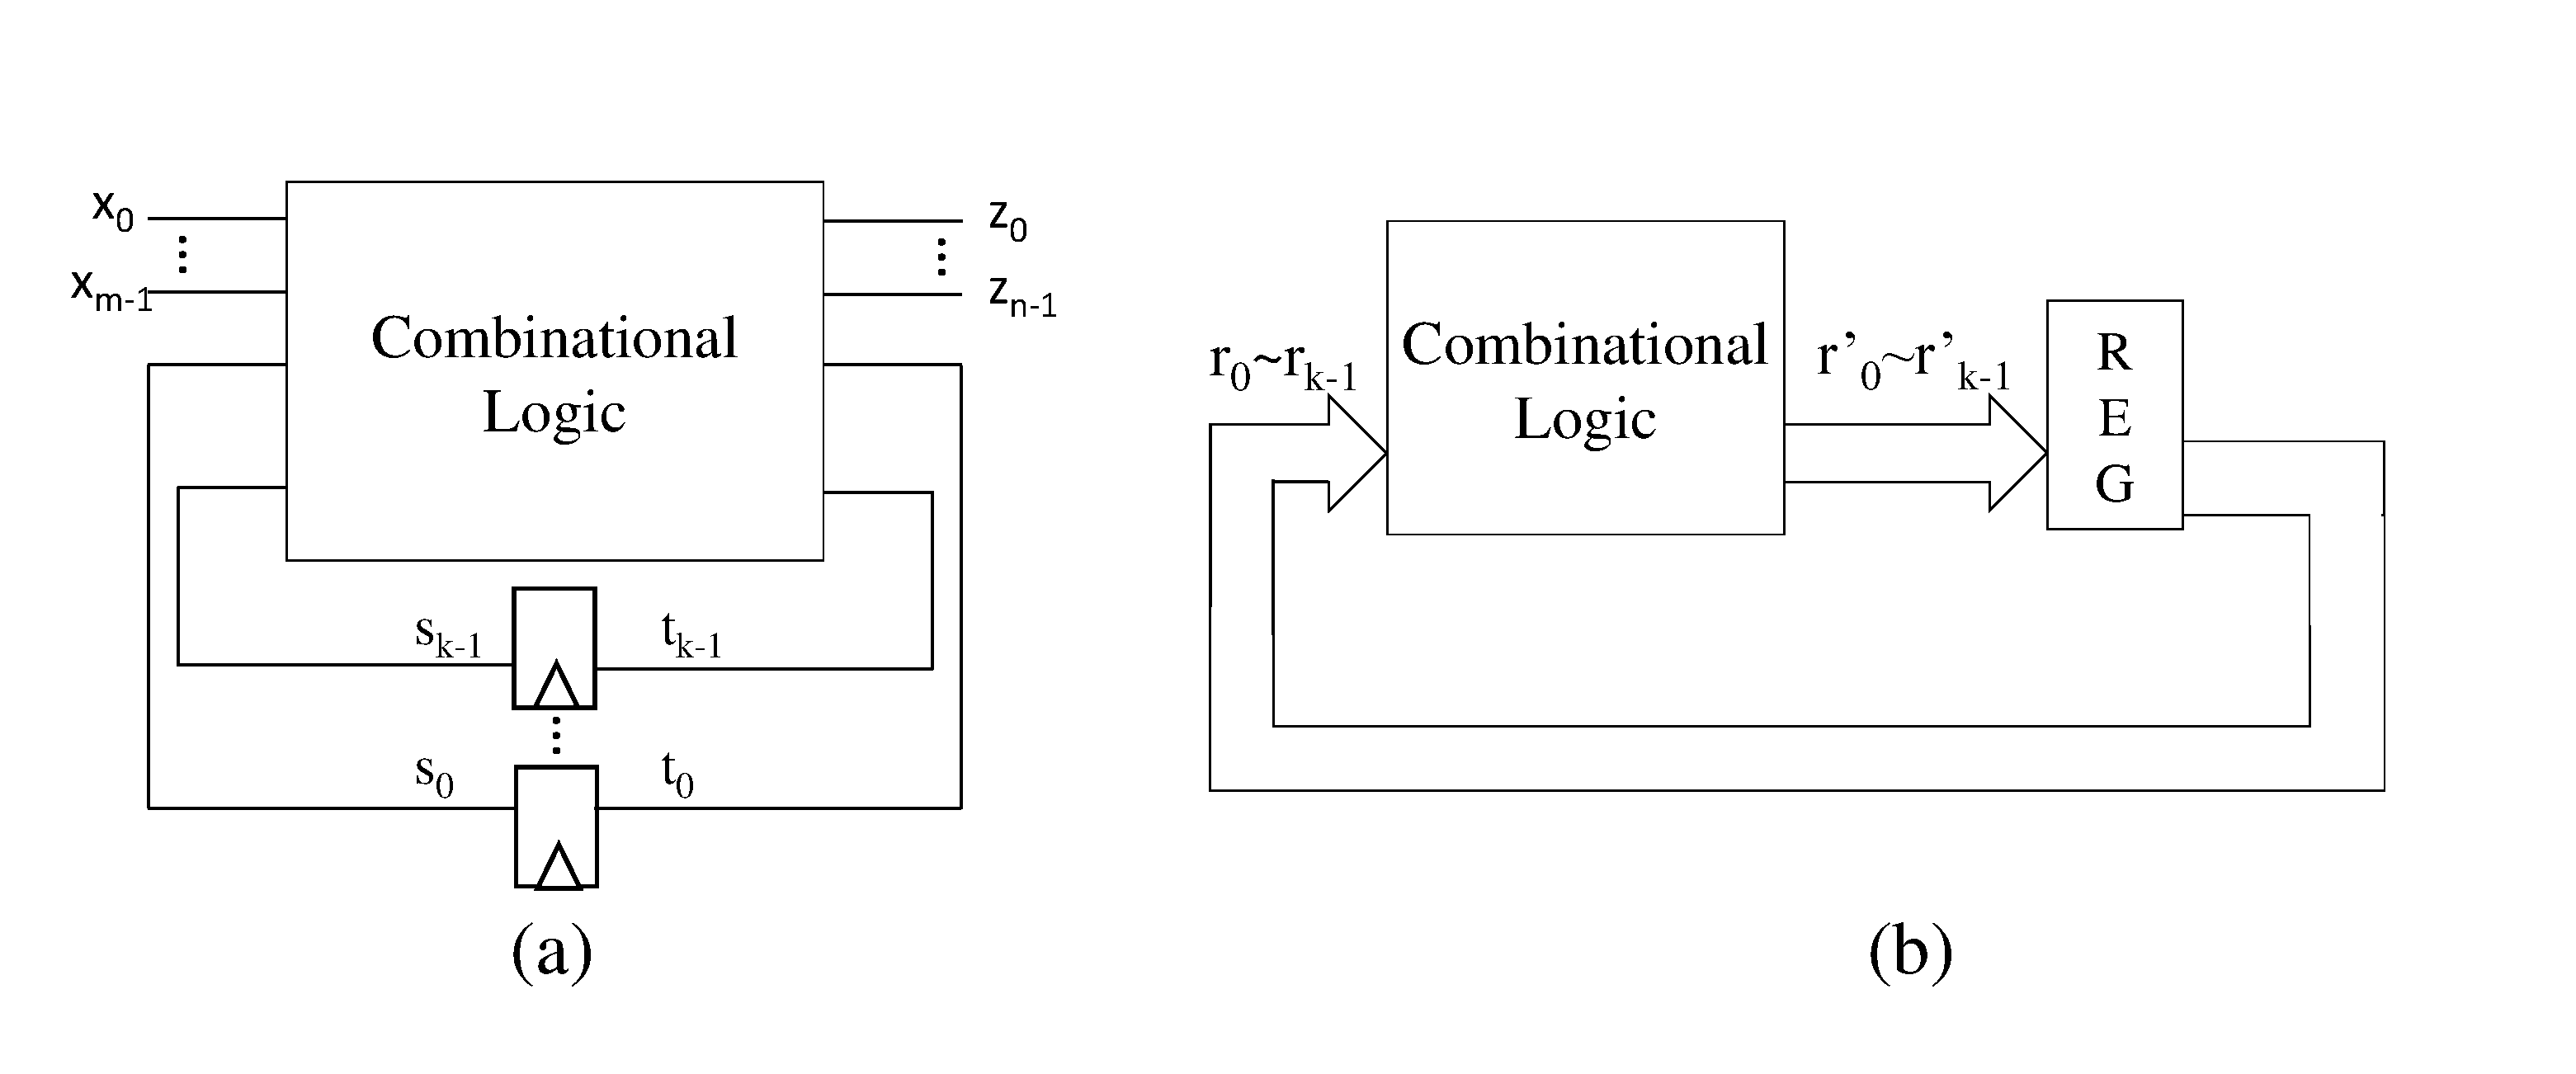
\includegraphics[width=5.5in]{newfig/seqmodel.pdf}
% \vspace{-0.2in}
\caption{FSM models of sequential circuits.}
%\end{minipage}
\label{fig:seqmodel}}
\end{figure}

\subsection{Conventional Traversal Method}
Conceptually, the state-space of a FSM is traversed in a breadth-first
manner, as shown in Algorithm \ref{alg:BFS}. % \cite{KallaPartialScan}: 
The algorithm operates on the FSM $\mathcal{M} = (\sum, O, S, S^0,
\Delta, \Lambda)$ underlying a sequential circuit. In such cases, the
transition function $\Delta$ and the initial states are represented
and manipulated using Boolean representations such as BDDs or SAT
solvers. The variables $from, reached, to, new$ represent
characteristic functions of sets of states. Starting from the initial
state $from^i = S^0$, the algorithm computes the states reachable in
1-step from $from^i$ in each iteration. In line 4 of Algorithm
\ref{alg:BFS}, the {\it image computation} is 
used to compute the reachable states in every execution step. 

The {\it transition function} $\Delta$ is given by Boolean equations
  of the flip-flops of the circuit: $t_i = \Delta_i(s, x)$, where
  $t_i$ is a next state variable, $s$ represents the present   state
  variables and $x$ represents the input variables. The {\it
    transition relation of the FSM} is then represented as:  
\begin{equation} 
T(s, x, t) =   \prod_{i=1}^{n} (t_i \overline{\oplus } \Delta_i)
\end{equation}
where $n$ is the number of flip flops, and $\overline{\oplus}$ is XNOR
operation. Let $from$ denote the set of initial states, then the
image of the initial states, under the transition function $\Delta$ is
finally computed as:
\begin{align}
\label{eqn:img}
to = \text{Img}(\Delta, from) = \exists _s ~\exists _x ~[ T(s, x, t)
  \cdot from ] 
%= \exists _s ~\exists _x ~\prod_{i=1}^{n} (t_i \overline{\oplus } \Delta_i)\cdot from
\end{align}

Here, $\exists x (f)$ represents the {\it existential quantification
  of $f$ {\it w.r.t.} variable $x$}. In Boolean logic, this operator is implemented as
  $$\exists x (f) = f_x\lor f_{\overline{x}}$$





Let us describe the application of the algorithm on the  FSM circuit
of Figure \ref{fig:fsm}. {\it We will first describe its operation at the
Boolean level, and then describe how this algorithm can be implemented
using algebraic geometry at word level.} 

\begin{figure}[bp]
\centering{
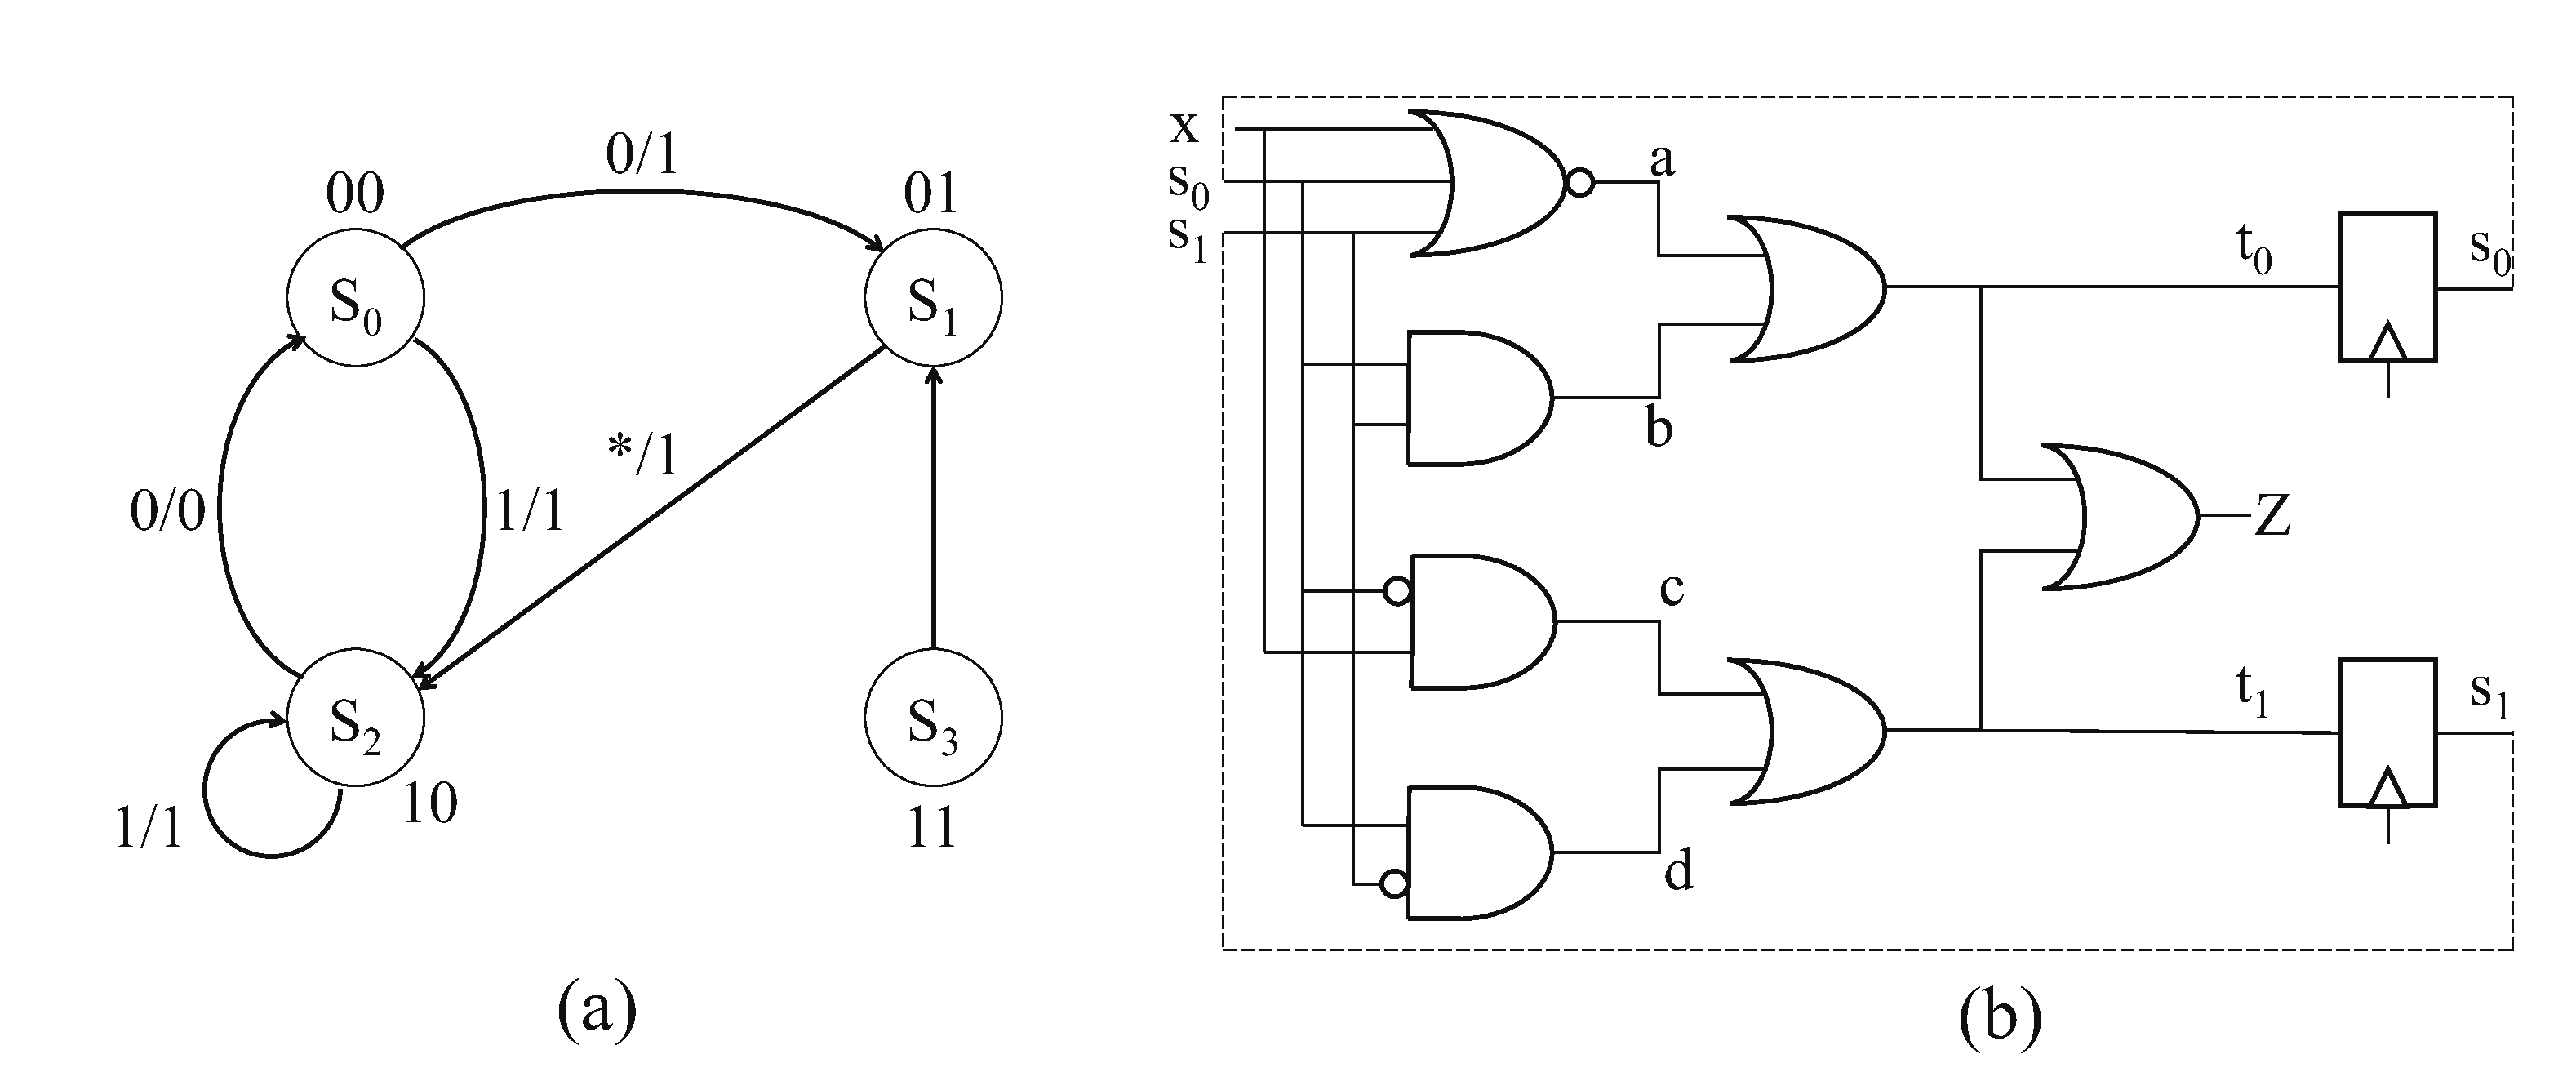
\includegraphics[width=\textwidth]{newfig/new_stg.eps}
\caption{The example FSM and the gate-level implementation. }
\label{fig:fsm}}
\end{figure}

In Line 1 of the BFS algorithm, assume that the initial state
is $S_3$ in Figure \ref{fig:fsm}(b), which is encoded as 
$S_3 = \{11\}$. Using Boolean variables $s_0, s_1$ for the present
states, $from^0 = s_0\cdot s_1$ is represented as a Boolean formula. 



\begin{Example}
For the circuit in Figure \ref{fig:fsm}(b), we have the transition
functions of the machine as:

\begin{align*}
\Delta_1: & ~t_0 \overline{\oplus} ((\overline{x \vee s_0 \vee s_1}) \vee s_0 s_1)\\
\Delta_2: & ~t_0 \overline{\oplus} (\overline{s_0}x \vee \overline{s_1}s_0)\\
from:     & ~from^0 = s_0\cdot s_1
\end{align*}

When the formula of Equation \ref{eqn:img} is applied to compute 1-step
reachability, $to = \exists _{s_0, s_1, x} (\Delta_1 \cdot \Delta_2
\cdot from^0)$, we obtain $to = \overline{t_0}\cdot t_1$, which denotes
the state $S_1 = \{01\}$ reached in 1-step from $S_3$.
In the next iteration, the algorithm uses state $S_1 = \{01\}$ as the
current (initial) state, and computes $S_2 = \{10\} = t_0\cdot
\overline{t_1}$ as the next reachable state, and so on. 
\end{Example}

%% Let  $\Delta_i$ denote the transition function for $i^{th}$ bit of the
%% output $T$
%% (denoted by $t_i$), and it is described by a Boolean function. We can
%% obtain the transition relation  for bit-vector $T$:
%% $Tran(s_0,s_1,x,t_0,t_1) =
%% \bigwedge_{i=1}^{2}(t_i\ \bar{\oplus}\ \Delta_i)$. Assume present
%% states are represent by Boolean formulas $PS(s_0,s_1)$, then the image
%% function is written as $\text{Img}(Tran,\ PS) =
%% \exists_{s_0,s_1}\exists_{x}[Tran(s_0,s_1,x,t_0,t_1)\land
%%   PS(s_0,s_1)]$, where $\exists_x f$ denotes the existential
%% quantification of $f$ w.r.t. $x$. 

Our objective is to model the transition functions $\Delta$ as a
polynomial ideal $J$, and to perform the image computations 
%(Algorithm \ref{alg:BFS}, line 4) 
using Gr\"obner bases over Galois fields. {\it
This requires to perform quantifier elimination; which can be
accomplished using the GB computation over $\Fkk$ using elimination
ideals} \cite{gao:qe-gf-gb}. Finally, the set union, intersection and
complement operations are also to be implemented in algebraic geometry.

\subsection{FSM Traversal at Word-Level over $\Fkk$} 
The state transition graph (STG) shown in Figure \ref{fig:fsm}(a) uses a
2-bit Boolean vector to represent 4 states $\{S_0, S_1, S_2,
S_3\}$. We map these states to elements in $\mathbb{F}_{2^2}$, where
$S_0 = 0, S_1 = 1, S_2 = \alpha, S_3 = \alpha+1$. Here, we take 
$P(X) = X^2+X+1$ as the irreducible polynomial to construct
$\mathbb{F}_4$, and $P(\alpha) = 0$ so that $\alpha^2 + \alpha + 1 =
0$.  

{\it Initial state:} Line 1 of Algorithm \ref{alg:BFS} specifies the initial state.
In algebraic geometry, it can be specified by means of a corresponding polynomial
 $f = \mathcal{F}(S) =
S - 1 - \alpha$. Notice that if we consider the ideal generated by the
initial state polynomial, $I = \langle f\rangle$, then its variety
$V(I) = 1+\alpha$ corresponds to the state encoding $S_3 = \{11\} =
1+\alpha$, where a polynomial in word-level variable $S$ encodes the
initial state. 
% with only one generator $f$, its variety
% $V(I) = \{\gamma\ |\ \gamma \in \mathbb{F}_{2^2}, \gamma = 1+\alpha\}$, which equals to $\{1+\alpha\}$, the only
% valid value $S_3$ can take.


%Using theorems from Section \ref{sec:elim}, we implement the image
%function by a GB computation on elimination ideal. Ex.\ref{ex:motiv}
%is an example for our implementation of image function, i.e. one-step
%reachability. 

{\bf Set operations:} In Lines 5 and 6 of
Algorithm  \ref{alg:BFS}, we need  \textbf{union}, 
\textbf{intersection} and \textbf{complement} of varieties over
$\mathbb{F}_{2^k}$, for which we again use algebraic geometry concepts.

\begin{Definition}
\label{def:sum}
({\bf Sum/Product of Ideals} \cite{ideals:book}) If $I = \langle f_1,
\dots, f_r\rangle$ and $J = \langle g_1, \dots, g_s\rangle$ are
ideals in $R$, then the {\bf sum} of $I$ and $J$ is defined as $I + J
= \langle f_1, \dots, f_r, g_1, \dots, g_s\rangle$. Similarly, the
{\bf product} of $I$ and $J$ is $I \cdot J = \langle
f_ig_j\ |\ 1 \leq i \leq r, 1 \leq j \leq s\rangle$. 
\end{Definition}

%With concepts of ideal sums and products, we can obtain the
%intersection and union of affine varieties as:
\begin{Theorem}
\label{thm:unionintersect}
If $I$ and $J$ are ideals in $R$, then 
${\bf V}(I + J) = {\bf V}(I) \bigcap {\bf V}(J)$ and ${\bf V}(I \cdot
J) = {\bf V}(I) \bigcup {\bf V}(J)$. 
\end{Theorem}


In Line 5 of Algorithm  \ref{alg:BFS}, we need to compute the complement of a
set of states. Assume that $J$ denotes a polynomial ideal whose
variety $V(J)$ denotes a set of states. We require the computation of
another polynomial ideal $J'$, such that $V(J')=\overline{V(J)}$. We
show that this computation can be performed using the concept of {\bf
  ideal quotient}:  

\begin{Definition}
\label{def:quo}
({\bf Quotient of Ideals}) If $I$ and $J$ are ideals in a ring $R$, then $I:J$ is the set
%  \begin{equation}
  $\{f \in R \ |\ f\cdot g \in I, \forall g \in J\}$ %\nonumber
%  \end{equation}
and is called the {\bf ideal quotient} of $I$ by $J$.
\end{Definition}

%The following example shows a simple ideal quotient operation:
\begin{Example}
In $\Fq[x,y,z]$, ideal $I = \langle xz,yz\rangle$, ideal $J = \langle z\rangle$. Then
\begin{align*}
I:J &= \{f\in\Fq[x,y,z]~|~f\cdot z \in \langle xz,yz\rangle\} \\
&= \{f\in\Fq[x,y,z]~|~f\cdot z = Axz+Byz\}\\
&= \{f\in\Fq[x,y,z]~|~f= Ax+By\}\\
&= \langle x,y\rangle
\end{align*}
\end{Example}

% However, complement of variety cannot be easily dealt by simple arithmetic on polynomial generators.
% For non-trivial cases we can only prove that 
% \begin{Theorem}
% Let $I, J$ be ideals in $\mathbb F[x_1,\dots,x_n]$, then 
% $${\bf V}(I:J) \supset {\bf V}({\bf I}({\bf V}(I) - {\bf V}(J)))$$
% \end{Theorem}
% Fortunately for most hardware verification cases, the form of polynomial generators are restricted.
% A proposition has been proved by \cite{jinpeng} that after adding {\bf vanishing polynomials ideal}
% the new composed ideal implies following corollary:

We can now obtain the complement of a variety through the following
results which are stated and proved below:

\begin{Lemma}
\label{lem:gcd}
Let $f,g\in \Fkk[x]$, then $\langle f:g\rangle = \left\langle\frac{f}{gcd(f,g)}\right\rangle$.
\end{Lemma}

\begin{Proof}
Let $d = gcd(f, g)$. So, $f = df_1 , g = dg_1$ with $gcd(f_1 , g_1 ) =
1$. Note that $f_1 = \frac{f}{gcd(f,g)}$.

Take $h \in \langle f : g\rangle$. According to the
Definition \ref{def:quo}, $hg \in \langle f \rangle$, which means $hg = f
\cdot r$ with $r \in \Fkk[x]$. Therefore, $hdg_1 = df_1 r$ and $hg_1 =
f_1 r$. But considering $gcd(g_1 , f_1 ) = 1$ we have the fact that
$f_1$ divides $h$. Hence $h \in \langle f_1\rangle$.

Conversely, let $h \in \langle f_1 \rangle$. Then $h = s \cdot f_1$,
where $s \in \Fkk[x]$. So, $hg = hdg_1 = sf_1 dg_1 = sg_1 f \in 
\langle f \rangle$. Therefore, $h \in \langle f : g\rangle$.
\end{Proof}


\begin{Theorem}
\label{thm:quotient}
Let $J$ be an ideal generated by a single univariate polynomial in
variable $x$ over $\Fkk[x]$, and let the vanishing ideal $J_0 = \langle
x^{2^k}-x\rangle$. Then  
$${ V}(J_0:J) = { V}(J_0) - { V}(J),$$ where all the varieties are
considered over the field $\Fkk$. 
\end{Theorem}

\begin{Proof}
Since $\Fkk[x]$ is a principal ideal domain, $ J = \langle g(x)\rangle$
for some polynomial $ g(x) \in \Fkk[x]$. Let $h(x) = gcd(g(x), x^{2^k} -
x)$. So, $g(x) = h(x)g_1(x) , x^{2^k} - x = h(x)f_1(x)$, with $gcd(f_1(x) , g_1(x) ) =
1$. Then $J_0 : J = \langle f_1(x) \rangle$ by Lemma \ref{lem:gcd}. 

Let $x \in V(J_0 ) - V(J)$. From the definition of set
complement, we get $x \in \Fkk$ while $g(x) \neq 0$.  

Since $x^{2^k} = x$, we see that either $h(x) = 0$ or $f_1 (x) =
0$. Considering $g(x) \neq 0$, we can assert that $h(x) \neq 0$. In
conclusion, $f_1 (x) = 0$ and $x \in V(f_1 )$. 

Now let $x \in V(f_1 )$, we get $f_1 (x) = 0$. So, $x^{2^k} - x = 0$
gives $x \in V(J_0) = \Fkk$ which  contains all elements in the
field. 

Now we make an assumption that $x \in V(g)$. Then $g(x) = 0 =
d(x)g_1(x)$ which means either $h(x) = 0$ or $g_1 (x) = 0$. 

If $g_1 (x) = 0$, then since $f_1 (x) = 0$ we get that $f_1(x) , g_1(x)$
share a root. This contradicts the fact that $gcd(f_1(x) , g_1(x) ) = 1$.

On the other hand, if $h(x) = 0$, then since $f_1 (x) = 0$ and
$x^{2^k} - x = d(x)f_1(x)$, we get that $x^{2^k} - x$ has a double root. 
But this is impossible since the derivative of $x^{2^k} - x$ is $-1$.

So, $x \notin V(g(x))$ and this concludes the proof.
\end{Proof}

% Let $J_0 = \langle x_1^{2^k} - x_1, \dots, x_n^{2^k} - x_n \rangle$
% denote the ideal of all vanishing polynomials in $\Fkk$. Then, we have
% $V(J_0) = (\Fkk)^{n}$; i.e. the variety of vanishing ideal contains
% all possible valuations of variables, so it constitutes the {\bf
%   universal set}. Subsequently, based on Theorem \ref{thm:quotient},
% the {\bf absolute complement} $V(J')$ of a variety $V(J)$ can be
% computed as: 

Let $x^{2^k}-x$ be a vanishing polynomial in $\Fkk[x]$. Then $V(x^{2^k}-x)=\Fkk$
{\it i.e.} the variety of vanishing ideal contains
 all possible valuations of variables, so it constitutes the {\bf
   universal set}. Subsequently, based on Theorem \ref{thm:quotient},
 the {\bf absolute complement} $V(J')$ of a variety $V(J)$ can be
 computed as: 

\begin{Corollary} \label{cor:complement}
Let $J\subseteq \Fkk[x]$ be an ideal, and $J_0=\langle x^{2^k}-x\rangle$. Let $J'$ be an ideal 
computed as $J' = J_0:J$. Then $$V(J') = \overline{V(J)} = {V}(J_0:J)$$
\end{Corollary}

With Corollary \ref{cor:complement}, we are ready to demonstrate the
concept of word-level FSM traversal over $\Fkk$ using algebraic
geometry. The algorithm is given in Algorithm \ref{alg:univa}. Note that in
the algorithm, $from^i, to^i, new^i$ are {\it univariate polynomials in variables $S$
or $T$} only, due to the fact that they are the result of a GB
computation with an elimination term order, where the bit-level 
variables are abstracted and quantified away.

\section{Problem Setup and Formulation}
\begin{Problem}
We use the notions from Figure \ref{fig:seqmodel}(a) in this setup. 
\begin{enumerate}[{1)}] 
\item The circuit is modeled over $\Fkk = \F_2[x]\pmod{p(x)}, p(\alpha) = 0$, where $k$ is the number of flip-flops,
	the PS variables $\{s_0,\dots,s_{k-1}\}$, NS variables $\{t_0,\dots,t_{k-1}\}$.
\item Denote $S$ as the PS word-level by the following polynomial:
$$f_S: S = s_0+s_1\alpha+s_2\alpha^2+\cdots+s_{k-1}\alpha^{k-1}$$
Similarly we define NS word-level variable $T$ by:
$$f_T: T = t_0+t_1\alpha+t_2\alpha^2+\cdots+t_{k-1}\alpha^{k-1}$$
\item Impose ATO for sequential circuits which is 
$$LEX: \text{ all bit-level variables in any order }>S>T$$
\item Write polynomials $f_1,\dots,f_s$ for each gate, and construct ideal describing the circuit:
$$J_{ckt} = \langle f_1,\dots,f_s,f_S,f_T\rangle$$
as well as the ideal with vanishing polynomials:
$$J_0 = \langle \dots,x_i^2-x_i,\dots,S^{2^k}-S,T^{2^k}-T\rangle$$
where $x_i$ corresponds to bit-level variables denoting wires in the circuit.
\item Compute GB with ATO for $G$. Then obtain the projection of variety only on NS variable $T$, by
$$G\cap \Fkk[T]$$
\end{enumerate}
\end{Problem}


% \IncMargin{1em}
\begin{algorithm}[hbt]
\SetAlgoNoLine
\LinesNumbered
% \Indm
 \KwIn{The circuit's characteristic polynomial ideal $J_{ckt}$,
   initial state polynomial $\F(S)$, and LEX term order: bit-level
   variables $x, s, t$ $>$ PS word $S$ $>$ NS word $T$}
% \Indp

  $from^0 = reached = \Func(S)$\;
  \Repeat{$\langle new^i\rangle == \langle 1\rangle$}
  {
  	$i \gets i + 1$\;
  	$G \gets$GB($\langle J_{ckt},J_v, from^{i-1}\rangle$)\;
  	\tcc{Compute Gr\"obner basis with elimination term order: $T$ smallest}
	$to^i \gets G\cap \Fkk[T]$\;
	\tcc{There will be a univariate polynomial in $G$ denoting the
          set of next states in word-level variable $T$}
	$\langle new^i\rangle \gets \langle to^i\rangle + (\langle T^{2^k}-T\rangle:\langle reached\rangle)$\;
	\tcc{Use quotient of ideals to attain complement of reached states, then use sum of ideals to attain an intersection with next state}
  	$\langle reached\rangle \gets \langle reached\rangle \cdot \langle new^i\rangle$\;
  	\tcc{Use product of ideals to attain a union of newly reached states and formerly reached states}
	$from^i \gets new^i(S\setminus T)$\;
	\tcc{Start a new iteration by replacing variable $T$ in newly reached states with current state variable $S$}
  }
  \tcc{Loop until a fixpoint reached: newly reached state is empty}
\Return{$\langle reached\rangle$}
\caption {Algebraic Geometry based FSM Traversal}\label{alg:univa}
\end{algorithm}
% \DecMargin{1em}

\subsection{Word-Level FSM Traversal Example}
\begin{Example}
\label{ex:SMPO}
We apply Algorithm \ref{alg:univa} to the example shown in
Figure \ref{fig:fsm} to execute the FSM traversal. Let the initial state
$from^0 = \{00\}$ in $\B^2$ or $0 \in \mathbb F_4$. Polynomially, it is
written as $from^0 = S - 0$. In the first iteration, we compose
an ideal $J$ with 

%\begin{minipage}[h]{0.4\textwidth}
\begin{align*}
&f_1: t_0- (xs_0s_1+xs_0+xs_1+x+s_0+s_1+1)\\
&f_2: t_1 - (xs_0+x+s_0s_1+s_0)\\
&f_3: S - s_0 - s_1\alpha; ~~~f_4: T - t_0 - t_1\alpha
\end{align*}
$J_{ckt} = \langle f_1,f_2,f_3,f_4\rangle$, and the vanishing
polynomials: 
%\end{minipage}
%\begin{minipage}[h]{0.6\textwidth}

\begin{align*}
&f_5: x^2-x; ~~f_6: s_0^2-s_0, ~~f_7: s_1^2-s_1\\
&f_8: t_0^2-t_0, ~~f_9: t_1^2-t_1; ~~f_{10}: S^4-S, ~~f_{11}:T^4-T
\end{align*}
with $J_v = \langle f_5,f_6,\dots,f_{11}\rangle$.
%\end{minipage}

%and $from^0$. 

Compute $G = GB(J)$ for $J = J_{ckt}+J_0+\langle from^0\rangle$,
with an elimination term order 
$$ \underbrace{\{x,s_0,s_1,t_0,t_1\}}_{\text{all bit-level variables}} 
> \underbrace{S}_{\text{(PS~word)}} > \underbrace{T}_{\text{(NS~word)}}.$$

The resulting GB $G$ contains a polynomial generator with only $T$ as
the variable. In Line 5, assign it to the next state $$to^1 =
T^2+(\alpha+1)T+\alpha.$$ Note that the roots or variety of
$T^2+(\alpha+1)T+\alpha$ is $\{1, \alpha\}$, denoting the states
$\{01,10\}$. 

Since the formerly reached state ``$reached = T$'', its complement is
computed using Corollary \ref{cor:complement} 
$$\langle T^4-T\rangle:\langle T\rangle
= \langle T^3+1\rangle.$$ 

$V(\langle T^3 + 1\rangle) = \{1, \alpha, \alpha+1\}$ denoting the states
$\{01,10,11\}$. Then the newly reached state set in this iteration is 
$$\langle T^3+1, T^2+(\alpha+1)T+\alpha \rangle = \langle
T^2+(\alpha+1)T+\alpha \rangle$$ We add these states 
to formerly reached states 
\begin{align*}
reach &= \langle T\rangle \cdot \langle T^2+(\alpha+1)T+\alpha \rangle \\
&= \langle T\cdot T^2+(\alpha+1)T+\alpha \rangle \\
&= \langle T^3+(\alpha+1)T^2+\alpha T\rangle
\end{align*}
 {\it i.e.} states $\{00,01,10\}$. We update the present states
for next iteration $$from^1 = S^2+(\alpha+1)S+\alpha.$$ 

In the second iteration, we compute the reduced GB with the same term
order for ideal $J = J_{ckt}+J_v+\langle from^1\rangle$. 
It includes a polynomial generator $$to^2 = T^2+\alpha T$$ denotes states
$\{00,10\}$. The complement of $reached$ is $$\langle T^4-T\rangle:\langle T^3+(\alpha+1)T^2+\alpha T\rangle
= \langle T + 1+\alpha\rangle$$ ({\it i.e.} states $\{11\}$). We compute the newly reached state 
$$\langle T^2+\alpha T, T+1+\alpha \rangle = \langle 1\rangle$$ 

Since the GB contains the unit ideal, it means the newly reached state
set is empty, thus a fix-point has been reached. The algorithm
terminates and returns $$reached = \langle T^3+(\alpha+1)T^2+\alpha
T\rangle$$ which, as a Gr\"obner basis of the elimination ideal,
canonically encodes the final reachable state set. 
\end{Example}

% {\it Significance of using GB:} A reduced GB is a unique, minimal and
% {\it canonical} representation of the circuit's function. Starting
% from a certain initial state and using a reduced GB to represent the
% transition function, reachable states can be computed and represented
% canonically. Then it becomes possible to identify  when a fixpoint
% is reached (termination of the algorithm) by performing an equality
% check of polynomial ideals. Moreover, the GB computation is also used
% as a quantification procedure. As the GB is computed w.r.t. an
% elimination term order with ``bit-level variables'' $>$
% ``present-state word'' $S$ $>$ ``next-state word'' $T$, the set of
% reachable states are encoded, canonically, using a univariate
% polynomial in $T$, quantifying away the rest of the variables. 

\subsection{Significance of using Algebraic Geometry and Gr\"obner Bases}
The essence of our approach is based on algebraic geometry and Gr\"obner basis concepts.
One the one hand, we use GB with elimination term ordering as an analog of image function.
As mentioned in Section \ref{sec:abstraction}, we construct the ideal $J+J_0$ to 
describe the circuit in Figure \ref{fig:proj_reacha} using algebraic geometry.
Given the present states, the next states are implicitly represented in the variety of 
the elimination ideal obtained by quantify away the remaining variables. 
This projects the variety on the NS output $T$ by eliminating all other variables.
This projection gives us the canonical representation of NS in a polynomial in $T$.

\begin{figure}[bp]
\centering{
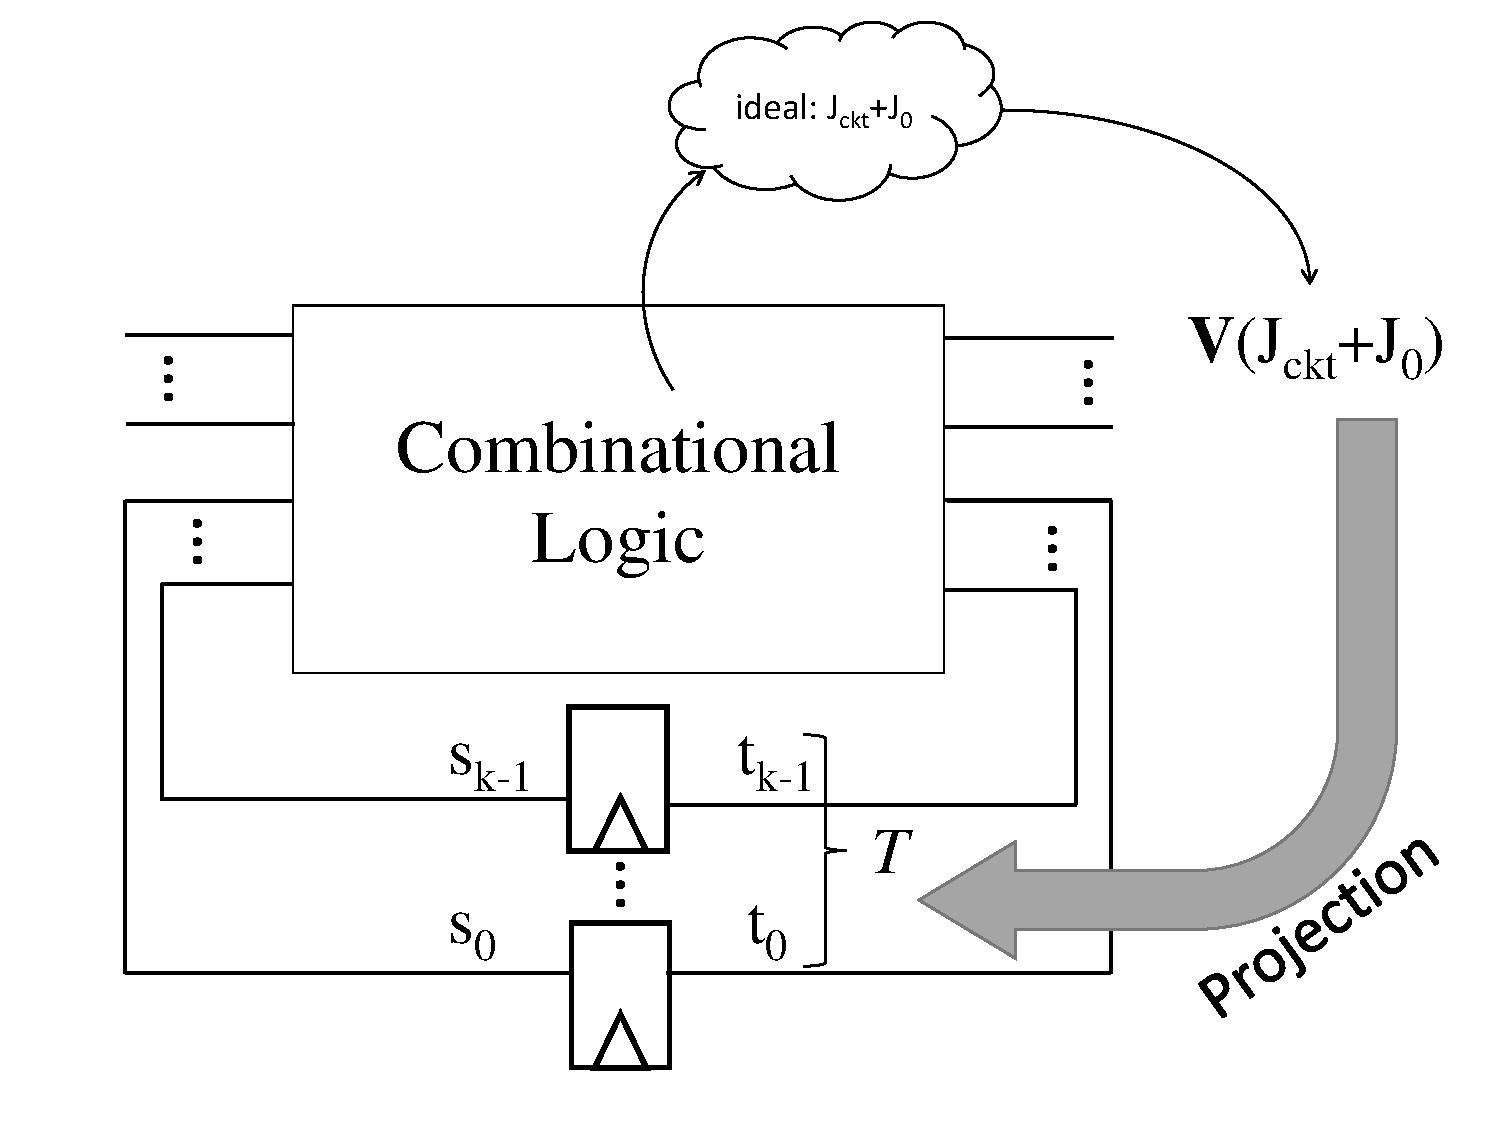
\includegraphics[width=\textwidth]{newfig/proj_reacha.pdf}
\caption{Projection of the variety of circuit description ideal.}
\label{fig:proj_reacha}}
\end{figure}

On the other hand, we use the algebraic ideals to implement set operations. States are finite set of points,
which can be mapped to a variety.
In algebraic geometry, manipulating the ideals provides a mechanism to 
operate on the varieties without actually solving the system of equations. The intersection, union and 
complement of varieties are mapped to varieties of the sum, product and quotient of ideals, respectively.
% Furthermore, the varieties are equivalent to set of states because of correspondence of 
% affine space and state space.

As a result, we create the analog of the FSM traversal algorithm in algebraic geometry which is 
compatible with word-level variables ({\it e.g.} $S,T$). We show it is effective to perform the 
reachability analysis.

\section{Improving our Approach}
\label{sec:improve}

Using elimination term ordering on computing GB for large set of polynomial is time-consuming, and usually 
intractable. The reason is the exponential computational complexity \cite{gao:gf-gb-ms}:
\begin{Theorem}
Let $J+J_0 = \langle f_1, \dots, f_s, ~x_1^q - x_1, \dots, x_d^q -
x_d\rangle \subset \Fq [x_1, \dots, x_d]$ be an ideal. The time and
space complexity of Buchberger's algorithm to compute a \Grobner
basis of $J+J_0$ is bounded by $q^{O(d)}$.
\end{Theorem}

In our case $q = 2^k$, and when $k$ and $d$ are large, this complexity 
makes abstraction infeasible.

Buchberger's algorithm consists of two major operations: one is finding 
$Spoly$ pairs, the other is dividing the $Spoly$ by the set of polynomials.
Its actual cost is very sensitive to the term ordering: if there exists 
a term order making most $Spoly$ computation unnecessary, then the cost to 
compute $Spoly$ is saved. Moreover, it prevents the generation of new polynomials 
from unnecessary $Spoly$ reductions, which further reduces the cost
because there are less $Spoly$ pairs as well as candidate divisors.
Besides tuning the term ordering, directly cutting down the number of 
polynomials in the set is also effective.

In order to make our approach scalable, we propose improvements from 
two aspects: 1) using another term ordering which can lower the 
computational complexity of obtaining GB; and 2) reducing the number of
polynomials by collecting bit-level primary inputs (PIs) and integrating them as word-level 
variables which are compatible with our working GF.

\subsection{Simplifying the Gr\"obner Bases Computation}
In Algorithm \ref{alg:univa}, a Gr\"obner basis is computed for each
iteration to attain the word-level polynomial representation of the next states. In practice, for 
a sequential circuit with complicated structure and large size, Gr\"obner basis computation
is intractable. To overcome the high computational complexity of computing a GB, 
we describe a method that computes a GB of a smaller subset of polynomials.
The approach draws inspirations from \cite{pruss:tcad15}, which defined and justified a 
{\it refined abstraction term order} (RATO). The following definition rephrases Definition 5.1 in \cite{pruss:tcad15}
with our sequential circuit setup and notations.

% From Tim's journal
\begin{Definition}[Refined Abstraction Term Order $>_r$]
Starting from the pseudo outputs (NS variables) of the combinational component of a sequential circuit $C$, 
perform a reverse topological 
traversal toward the pseudo inputs (PS variables) and primary inputs. Order each variable of the circuit according to
its reverse topological order. Impose a LEX term order $>_r$ on $\Fq[x_1,\dots,x_d,T,S]$
with the ``bit-level variables $x_1,\dots,x_d$ ordered reverse topologically "$ > T>S$,
this term order is called RATO.
\end{Definition}


According to proposition 5.1 in \cite{pruss:tcad15}, if the GB is computed using RATO, 
there will be only one pair of polynomials $\{f_w,f_g\}$ such that 
their leading monomials are not relatively prime, {\it i.e.} 
$$gcd(LM(f_w), LM(f_g)) \neq 1$$
As a well-known fact from Buchberger's algorithm, the S-polynomial 
($Spoly$) pairs with relatively prime 
leading monomials will always reduce to 0 modulo the basis and have no contribution to 
the Gr\"obner basis computation.
Therefore, by removing the polynomials with relatively prime leading terms from $J_{ckt}$, 
the Gr\"obner basis computation is transformed to the reduction of 
$Spoly(f_w,f_g)$ modulo $J_{ckt}$. More specifically, we turn the
GB computation into one-step multivariate polynomial division, and the obtained
remainder $r$ will only contain bit-level inputs and word-level output. 

\begin{Example}
In this example, we impose RATO on the polynomial ideal generated from the circuit in Figure \ref{fig:fsm}(b).
We start from the outputs $t_0,t_1$, then intermediate bit-level signals $a,b,c,d$ because they are 
the fanins of the corresponding gates which fanout $t_0,t_1$. Then we ends at the pseudo inputs $s_0,s_1$
and primary input $x$.
Thus variables in $J_{ckt}$ can be ordered by LEX with:
\begin{align}
&(t_0,t_1)>(a,b,c,d)>(x,s_0,s_1)\nonumber\\&>T>S\nonumber
\end{align}
This is the RATO for circuit in Figure \ref{fig:fsm}(b).

We can write down all polynomial generators of $J_{ckt}$:
\begin{equation*}
f_1: a+xs_0s_1+xs_0+xs_1+x+s_0s_1+s_0+s_1+1
\end{equation*}
\vspace{-0.8cm}
\begin{alignat*}{3}
& f_2: b+s_0s_1 &&~~~ f_3: c+x+xs_0 \\
& f_4: d+s_0s_1+s_0 &&~~~ f_5: t_0+ab+a+1 \\
& f_6: t_1+cd+c+d &&~~~ f_7: t_0+t_1\alpha+T 
\end{alignat*}

From observation, the only pair which is not relatively prime is
$(f_5,f_7)$, thus the critical candidate polynomial pair is
$(f_w,f_g)$, where $$f_w =f_5= t_0+a\cdot b+a+b, ~~f_g =f_7=t_0+t_1\alpha + T$$
Result after reduction is:
\begin{align}
&Spoly(f_w,f_g) \xrightarrow{J+J_0}_{+}T + s_0 s_1 x+\alpha s_0 s_1 \nonumber\\
&+(1+\alpha)s_0 x+(1+\alpha) s_0+s_1 x+s_1+(1+\alpha) x+1\nonumber
\end{align}
The remainder contains only bit-level inputs $(x,s_0,s_1)$ and word-level output $T$.
\end{Example}


The remainder from $Spoly$ reduction contains bit-level PS variables, and our objective is to get a polynomial 
containing only word-level PS variables. One possible method is 
to rewrite bit-level variables in term of word-level variables, {\it i.e.}
\begin{equation}
\label{eqn:BLVS_reacha}
s_i = \mathcal{G}(S)
\end{equation}

Then we can substitute all bit-level variables with the word-level variable
and obtain a word-level expression.
The authors of \cite{pruss:tcad15} propose a method to construct 
a system of equations, such that the solution to the system consists of Equation \ref{eqn:BLVS_reacha}.
It relies on a lemma which can be derived from Fermat's Little Theorem:
\begin{Lemma}
\label{lem:Fermat}
For elements $\alpha_i$ in $\Fkk$, the following equation holds ($n\geq 0$):
$$(\alpha_1+\alpha_2+\cdots+\alpha_t)^{2^n} = \alpha_1^{2^n}+\alpha_2^{2^n}+\cdots+\alpha_t^{2^n}$$
\end{Lemma}

Solution to the system of equations can be obtained by Gaussian elimination, which could 
compute corresponding $\mathcal{G}(S)$ efficiently with time complexity $O(k^3)$.

\begin{Example}
{\bf Objective}:\ Abstract polynomial $s_i + \mathcal{G}_i(S)$ from $f_0: s_0+s_1\alpha+S$.

First, compute $f_0^2: s_0+s_1\alpha^2+S^2$. Apparently variable $s_0$ can be
eliminated by operation 
\begin{align}
f_1 =& f_0 + f_0^2 \nonumber\\
=&(\alpha^2+\alpha)s_1+S^2+S\nonumber
\end{align}
Now we can solve univariate polynomial equation $f_1 = 0$ and get solution
$$s_1 = S^2 + S$$
Using this solution we can easily solve equation $f_0 = 0$. The result is
$$s_0 = \alpha S^2+(1+\alpha)S$$
\end{Example}

More formally, polynomial expressions for $s_i$ in terms of $S$ can be
obtained by setting up and solving the following system of equations:
\begin{align}
\label{eqn:alphamat}
\begin{bmatrix}
S \\
S^2 \\
S^{2^2} \\
\vdots \\
S^{2^{k-1}}
\end{bmatrix}
&=
\begin{bmatrix}
1 & \alpha & \alpha^{2} & \cdots & \alpha^{{k-1}}\\
1 & \alpha^{2} & \alpha^{4} & \cdots & \alpha^{2(k-1)} \\
1 & \alpha^{4} & \alpha^{8} & \cdots & \alpha^{4(k-1)}\\
\vdots & \vdots & \vdots & \ddots & \vdots \\
1 & \alpha^{2^{k-1}} & \alpha^{2\cdot 2^{k-1}} & \cdots & \alpha^{(k-1)\cdot 2^{k-1}}
\end{bmatrix}
\begin{bmatrix}
s_0\\
s_1\\
s_2\\
\vdots\\
s_{k-1}
\end{bmatrix}
\end{align}
Let $\vec{S}$ be a vector of $k$ unknowns $(s_0,\dots,s_{k-1})$,
then Equation \ref{eqn:alphamat} can be solved by using Cramer's rule or Gaussian elimination.
In other words, we can obtain $s_i=\mathcal G(S)$ by solving Equation \ref{eqn:alphamat} symbolically.

In this approach we get word-level variable representation for each bit-level PS variables. 
By substitution, a new polynomial in word-level PS/NS variables could be obtained.

After processing with RATO and bit-to-word conversions, we get a polynomial in the 
form of $f_T = T+\mathcal{F}(S,x)$
denoting the {\bf transition function}. We include a polynomial in $S$ to define the present states $f_S$,
as well as the set of vanishing polynomials for primary inputs 
$J_0^{PI} = \langle x_1^2-x_1,\dots,x_d^2-x_d\rangle$. Using elimination term order with $S>x_i>T$,
we can compute a GB of the elimination ideal $\langle f_T,f_S\rangle + J_0^{PI}$. This GB contains a univariate
polynomial denoting next states. The improved algorithm is depicted in Algorithm \ref{alg:refined}.

% \IncMargin{1em}
\begin{algorithm}[hbt]
\SetAlgoNoLine
\LinesNumbered
% \Indm
 \KwIn{Input-output circuit characteristic polynomial ideal $J_{ckt}$, initial state polynomial $\Func(S)$}
 \KwOut{Final reachable states represented by polynomial $\mathcal G(T)$}
% \Indp

  $from^0 = reached = \Func(S)$\;
  $f_T = $Reduce($Spoly(f_w,f_g), J_{ckt})$\;
  \tcc{Compute $Spoly$ for the critical pair, then reduce it with circuit ideal under RATO}
	Eliminate bit-level variables in $f_T$\;
  \Repeat{$\langle new^i\rangle == \langle 1\rangle$}
  {
  	$i \gets i + 1$\;
  	$G \gets$GB($\langle f_T , from^{i-1}\rangle+J_0^{PI}$)\;
  	\tcc{Compute Gr\"obner basis with elimination term order: $T$ smallest; $J_0^{PI}$ covers all possible inputs from PIs}
	$to^i \gets G\cup \Fkk[T]$\;
	\tcc{There will be a univariate polynomial in $G$ denoting next state in word-level variable $T$}
	$\langle new^i\rangle \gets \langle to^i\rangle + (\langle T^{2^k}-T\rangle:\langle reached\rangle)$\;
	\tcc{Use quotient of ideals to attain complement of reached states, then use sum of ideals to attain an intersection with next state}
  	$\langle reached\rangle \gets \langle reached\rangle \cdot \langle new^i\rangle$\;
  	\tcc{Use product of ideals to attain a union of new reached states and formerly reached states}
	$from^i \gets new^i(S\setminus T)$\;
	\tcc{Start a new iteration by replacing variable $T$ in new reached states with current state variable $S$}
  }
  \tcc{Loop until a fix-point reached: newly reached state is empty}
\Return{$\langle reached\rangle$}
\caption {Refined Algebraic Geometry based FSM Traversal}\label{alg:refined}
\end{algorithm}
% \DecMargin{1em}

\subsection{Primary Inputs Partitioning}
Using above techniques we can get a remainder polynomial with only word-level PS/NS variables. However in most 
cases, the number of bit-level PIs will be too large for the last-step Gr\"obner basis computation. 
Therefore it is necessary to convert bit-level PIs to word-level PI variables. 

As in Figure \ref{fig:PI}, assume there exist $k$-bit datapath and $n$-bit PIs. In finite field, we need to carefully partition $n$ PIs
such that states of each partition can be covered by a univariate polynomial respectively.

\begin{figure}[hbt]
\centering{
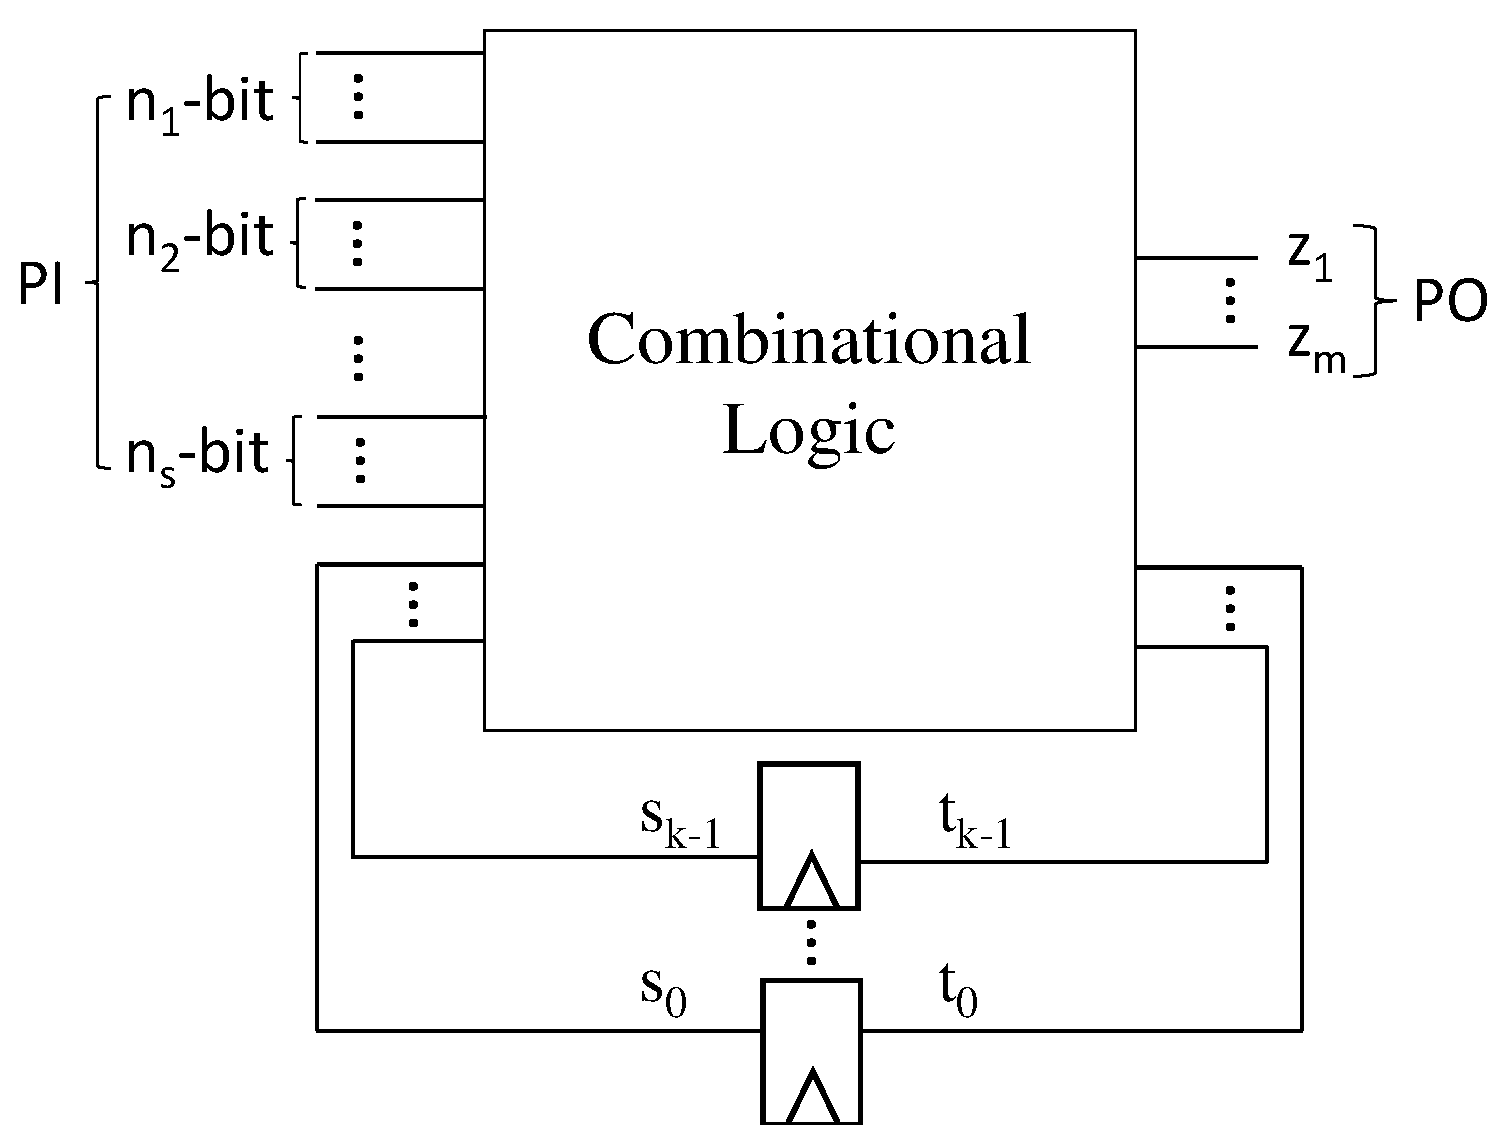
\includegraphics[width=\textwidth]{newfig/PI.pdf}
\caption{PI partition of a sequential circuit.}
\label{fig:PI}}
\end{figure}

\begin{Proposition}
Divide $n$-bit PIs into partitions $n_1,n_2,\dots, n_s$ where each $n_i|k$. Then let $n_1$-bit, $n_2$-bit, $\dots$, $n_s$-bit word-level variables
represent their evaluations in $\mathbb F_{2^k}$ as $\F_{2^{n_i}} \subset \Fkk$.
\end{Proposition}

Again, assume a partition $n_i~|~k$ and corresponding word-level variable is $P$. Then we can use polynomial
$P^{2^{n_i}}-P$ to represent all signals at free-end PIs, according to following theorem about {\bf composite
fields} \cite{ecc:software}:
\begin{Theorem}
\label{thm:composite}
Let $k = m\cdot n_i$, such that $\mathbb F_{2^k} = \mathbb F_{(2^{n_i})^m}$. Let $\alpha$ be primitive root of 
$\mathbb F_{2^k}$, $\beta$ be primitive root of the ground field $\mathbb F_{2^{n_i}}$. Then
$$\beta = \alpha^\omega,~~\text{where}~~\omega = \frac{2^k-1}{2^{n_i}-1}$$
\end{Theorem}
\begin{Example}
\label{ex:PI}
In a sequential circuit, PS/NS inputs/outputs are 4-bit signals, which means we will use $\mathbb F_{2^4}$
as working field. PIs are partitioned to 2-bit vectors, which means the ground field is $\mathbb F_{2^2}$.
In ground field we can represent all possible evaluations of this PI partition $\{p_0,p_1\}$ with
$$P^4+P,~~\text{where}~~P=p_0+p_1\cdot\beta$$
Using Theorem \ref{thm:composite} we get $\beta = \alpha^5$, so we can redefine word $P$ as element from $\mathbb F_{2^4}$:
$$P = p_0 + p_1\cdot\alpha^5$$
\end{Example}
Using this method we can efficiently partition large size PIs to small number of word-level PI variables.
One limitation of this approach is PIs cannot be partitioned when $k$ is prime.

\section{Implementation of Word-Level FSM Traversal Algorithm}
In this section, we describe the architecture of our tool which can perform word-level FSM traversal
on FSM benchmark circuits. Our tool consists of 3 functional components.
% First, the given circuit is synthesized to gate-level using state-of-art synthesizers.
First, the gate-level netlist of circuit is translated to polynomial form and variables are sorted in 
RATO. This part is implemented using a scripting language such as \emph{Perl}. If 
the given benchmark is a structural/behavior hybrid description, we perform pre-processing on it to get a synthesized netlist.
Secondly, the polynomial reduction is executed using our customized reduction engine, which is written in C++.
Finally, we utilize the symbolic computation engine \textsc{Singular} \cite{DGPS} to code Algorithm 
\ref{alg:refined} and execute the BFS traversal. The tool outputs a univariate polynomial 
for NS word $T$, denoting the set of reachable states from given initial state.

Figure \ref{fig:flowchart} illustrates the execution of reachability analysis approach
based on C++ and \textsc{Singular} implementation.

\begin{figure}[bp]
\centering{
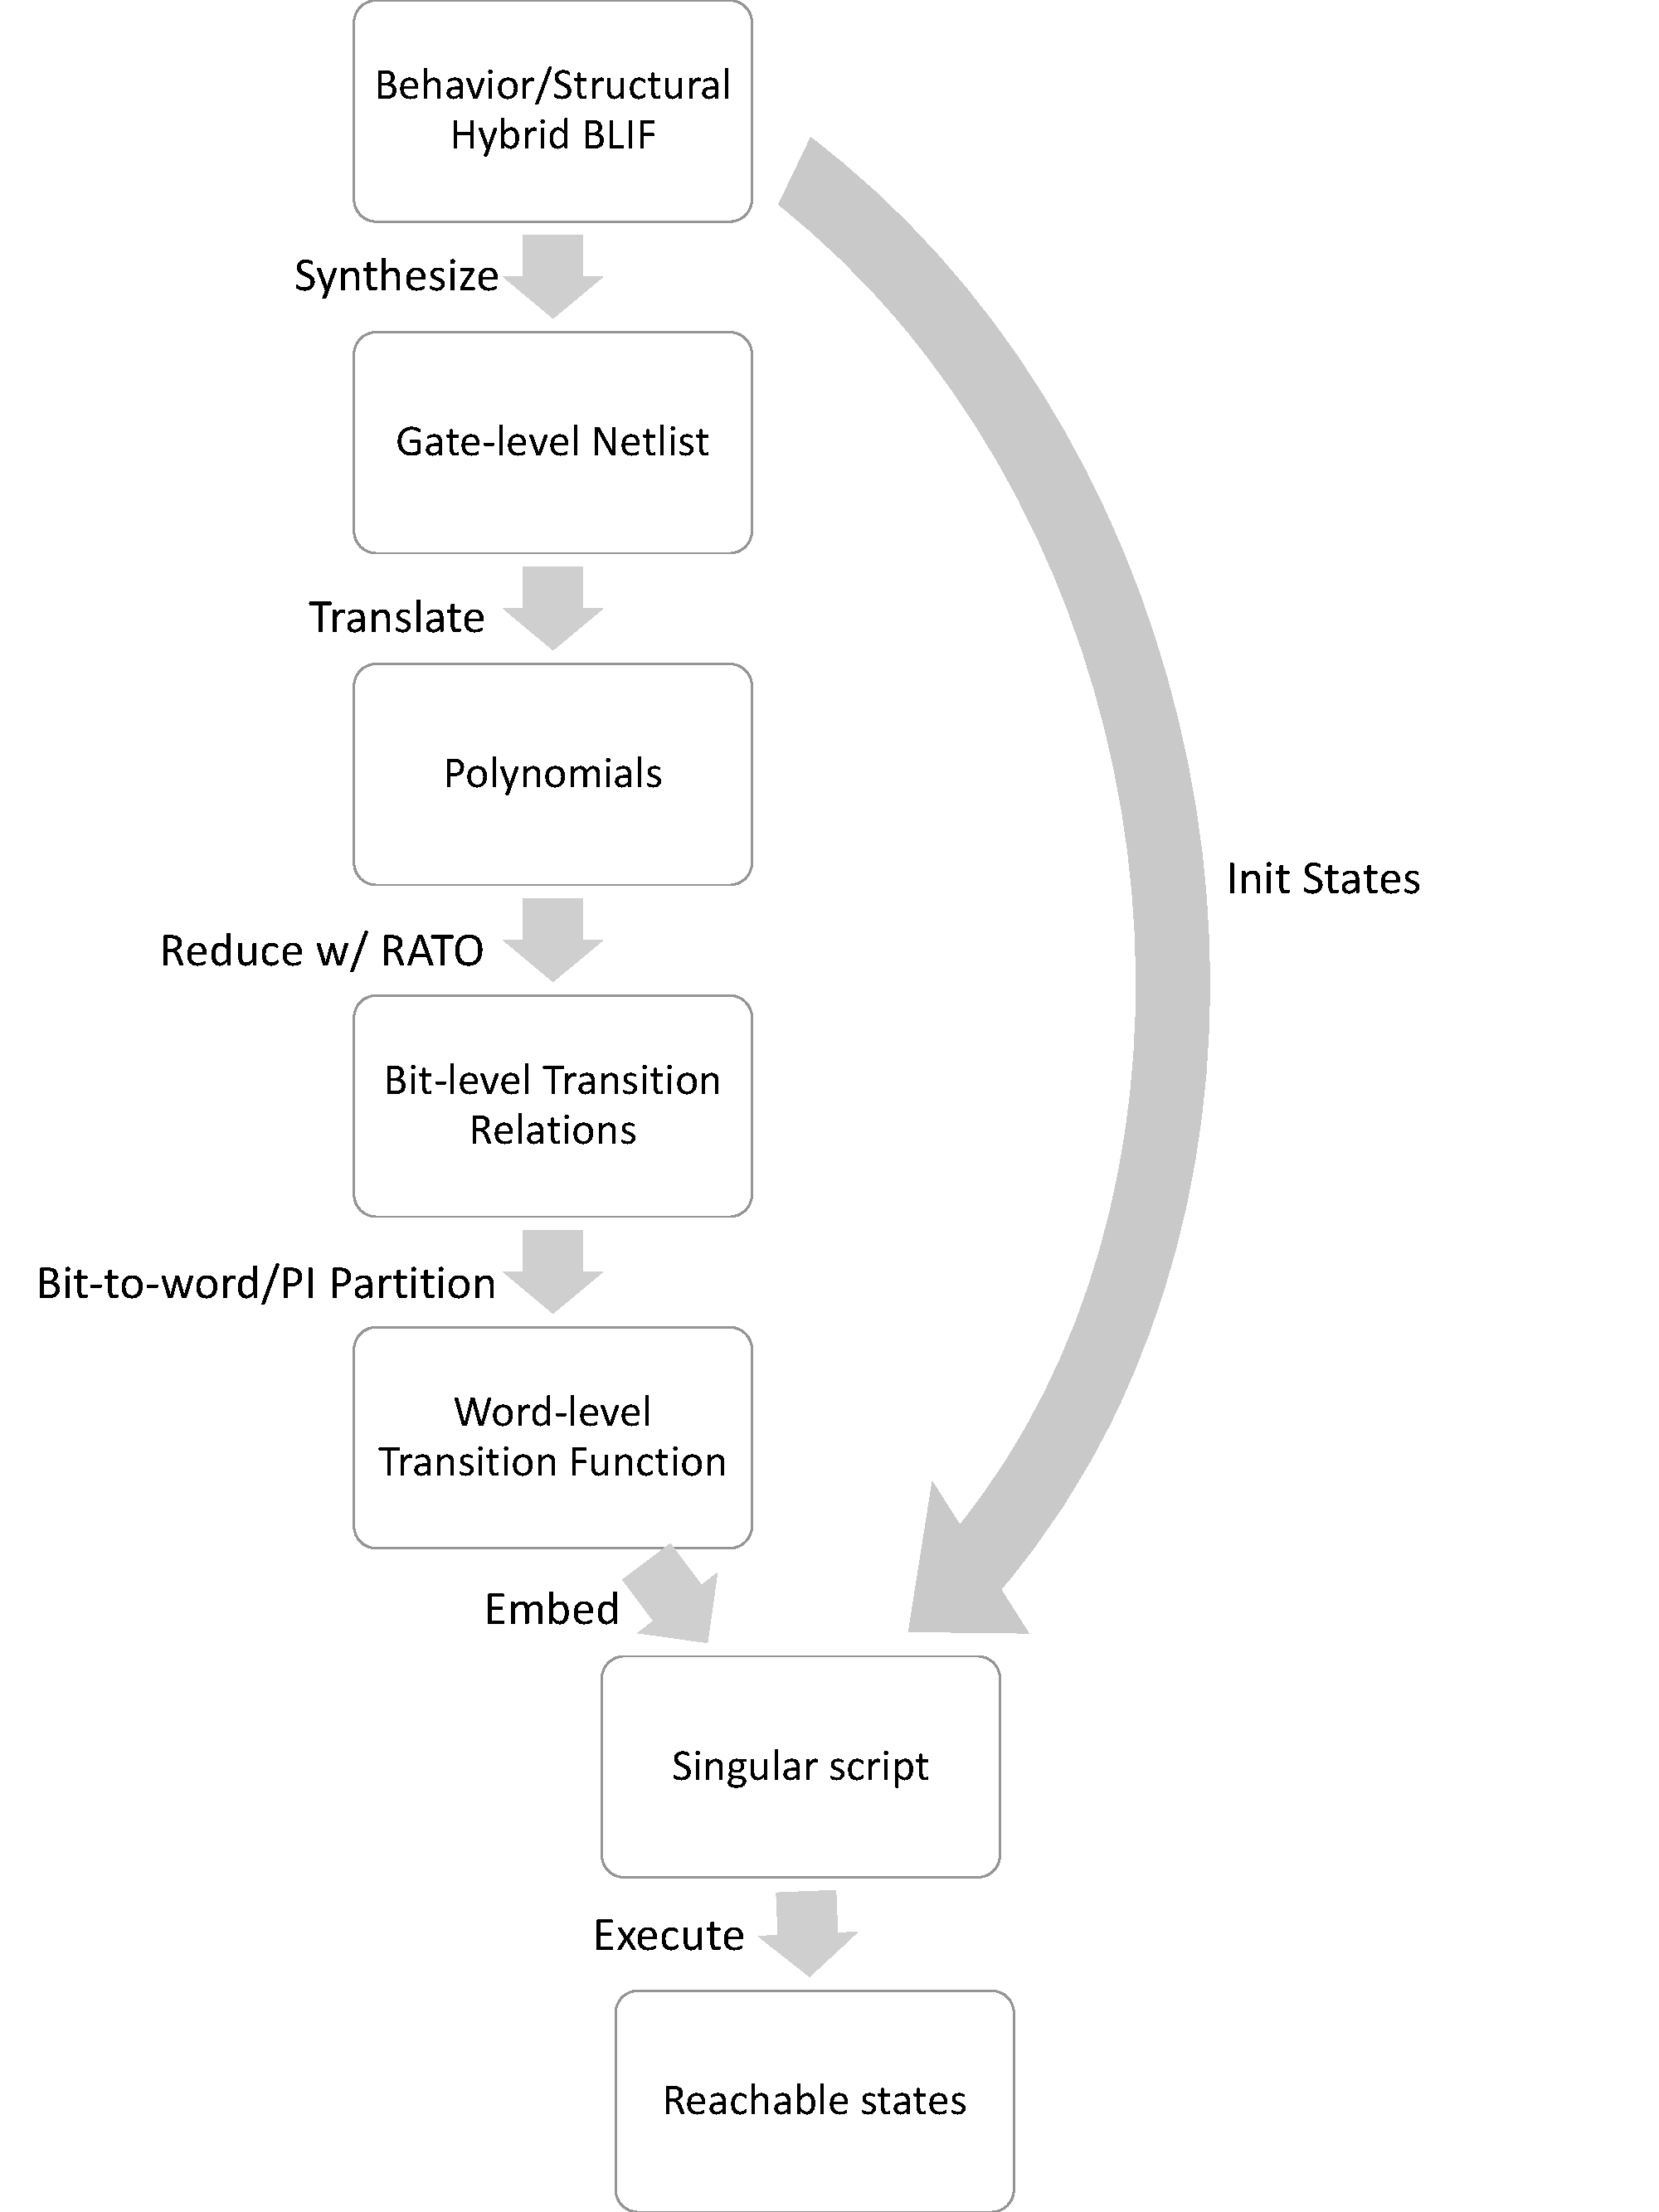
\includegraphics[width=\textwidth]{newfig/flowchart.pdf}
\caption{Execution process of word-level FSM traversal tool.}
\label{fig:flowchart}}
\end{figure}

Usually FSM designs can be described in behavior/structural hybrid languages.
One of these languages is the Berkeley logic interchange format (BLIF) \cite{BLIF},
it allows state behavior representation and logic component representation.

\begin{Example}
In this example, we use benchmark FSM ``lion9" from MCNC benchmark library.
This benchmark circuit is given as state table based BLIF representation of a FSM.

% \begin{figure}[hbt]
% \centering{
% 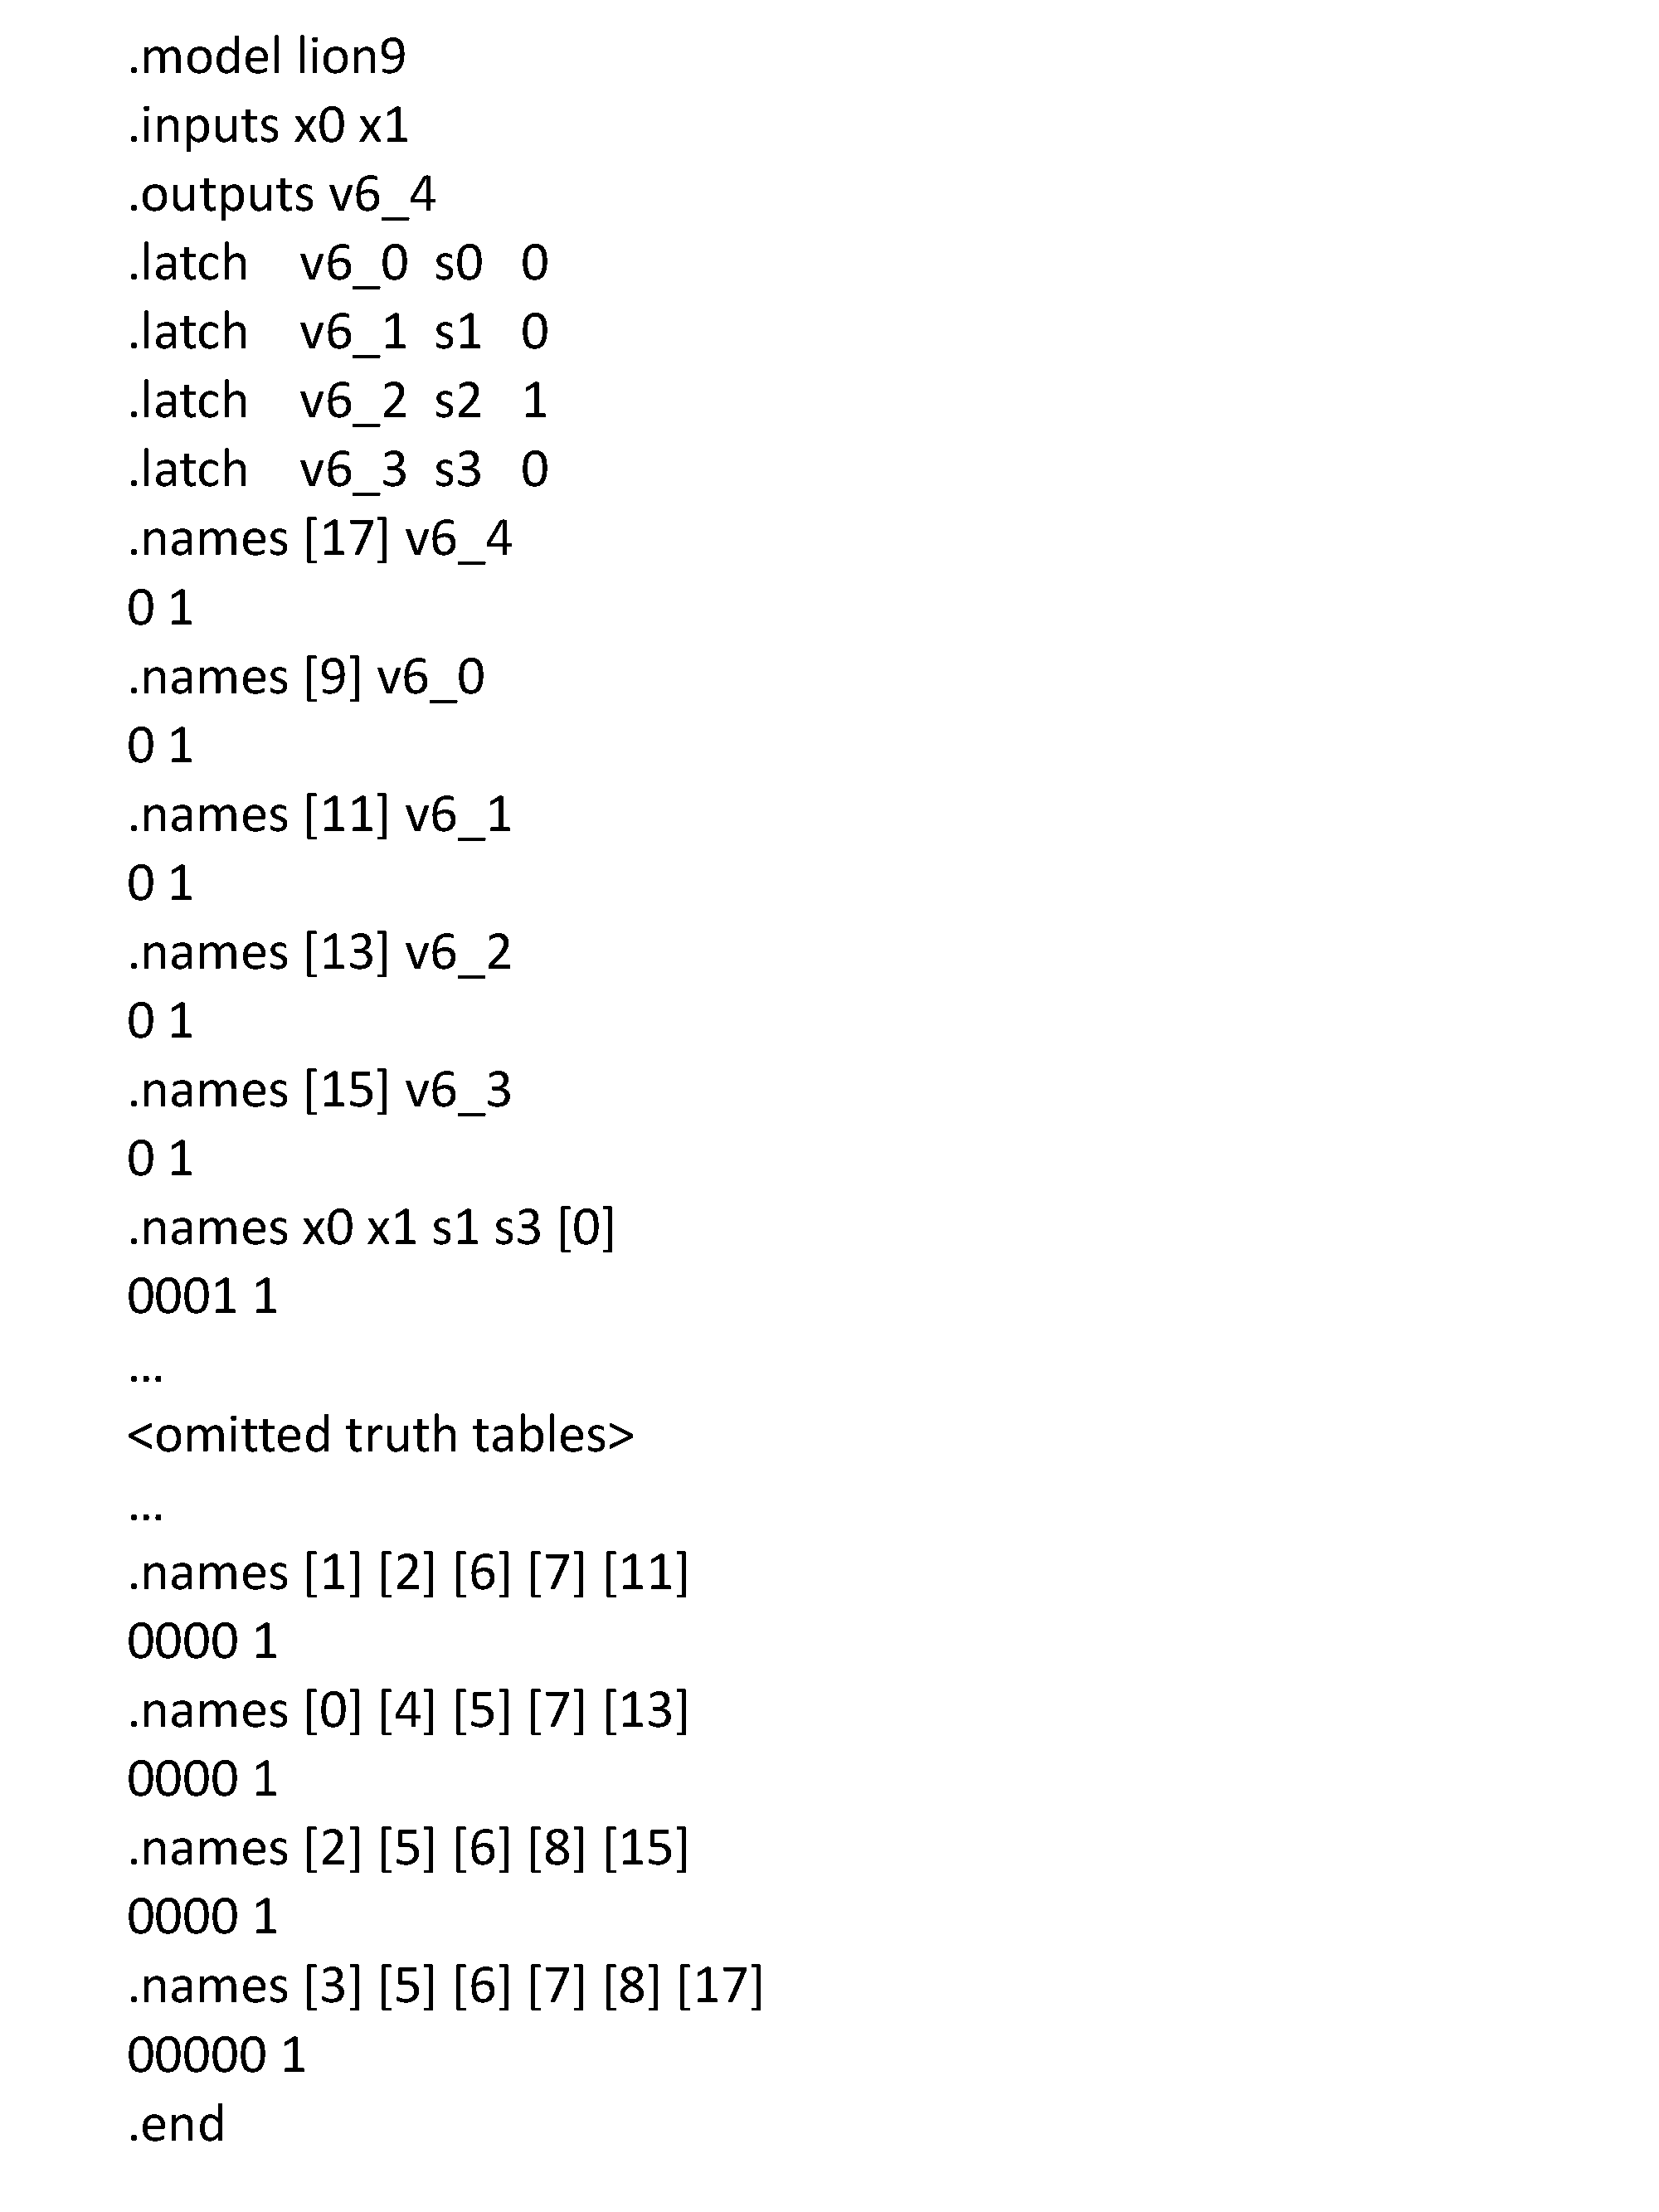
\includegraphics[width=\textwidth]{newfig/BLIF.pdf}
% \caption{Sample input BLIF file}
% \label{fig:BLIF}}
% \end{figure}

In order to compose the polynomial set in elimination ideal, we need to synthesize it to a 
gate-level netlist. Modern synthesizers including ABC \cite{brayton2010abc} and SIS \cite{SIS} 
can perform this task. In this example we use a synthesis library containing only 2-input 
AND, NAND, OR, NOR, XOR, XNOR gates as well as the inverter, the synthesized FSM is also given in 
BLIF format.

% \begin{figure}[hbt]
% \centering{
% 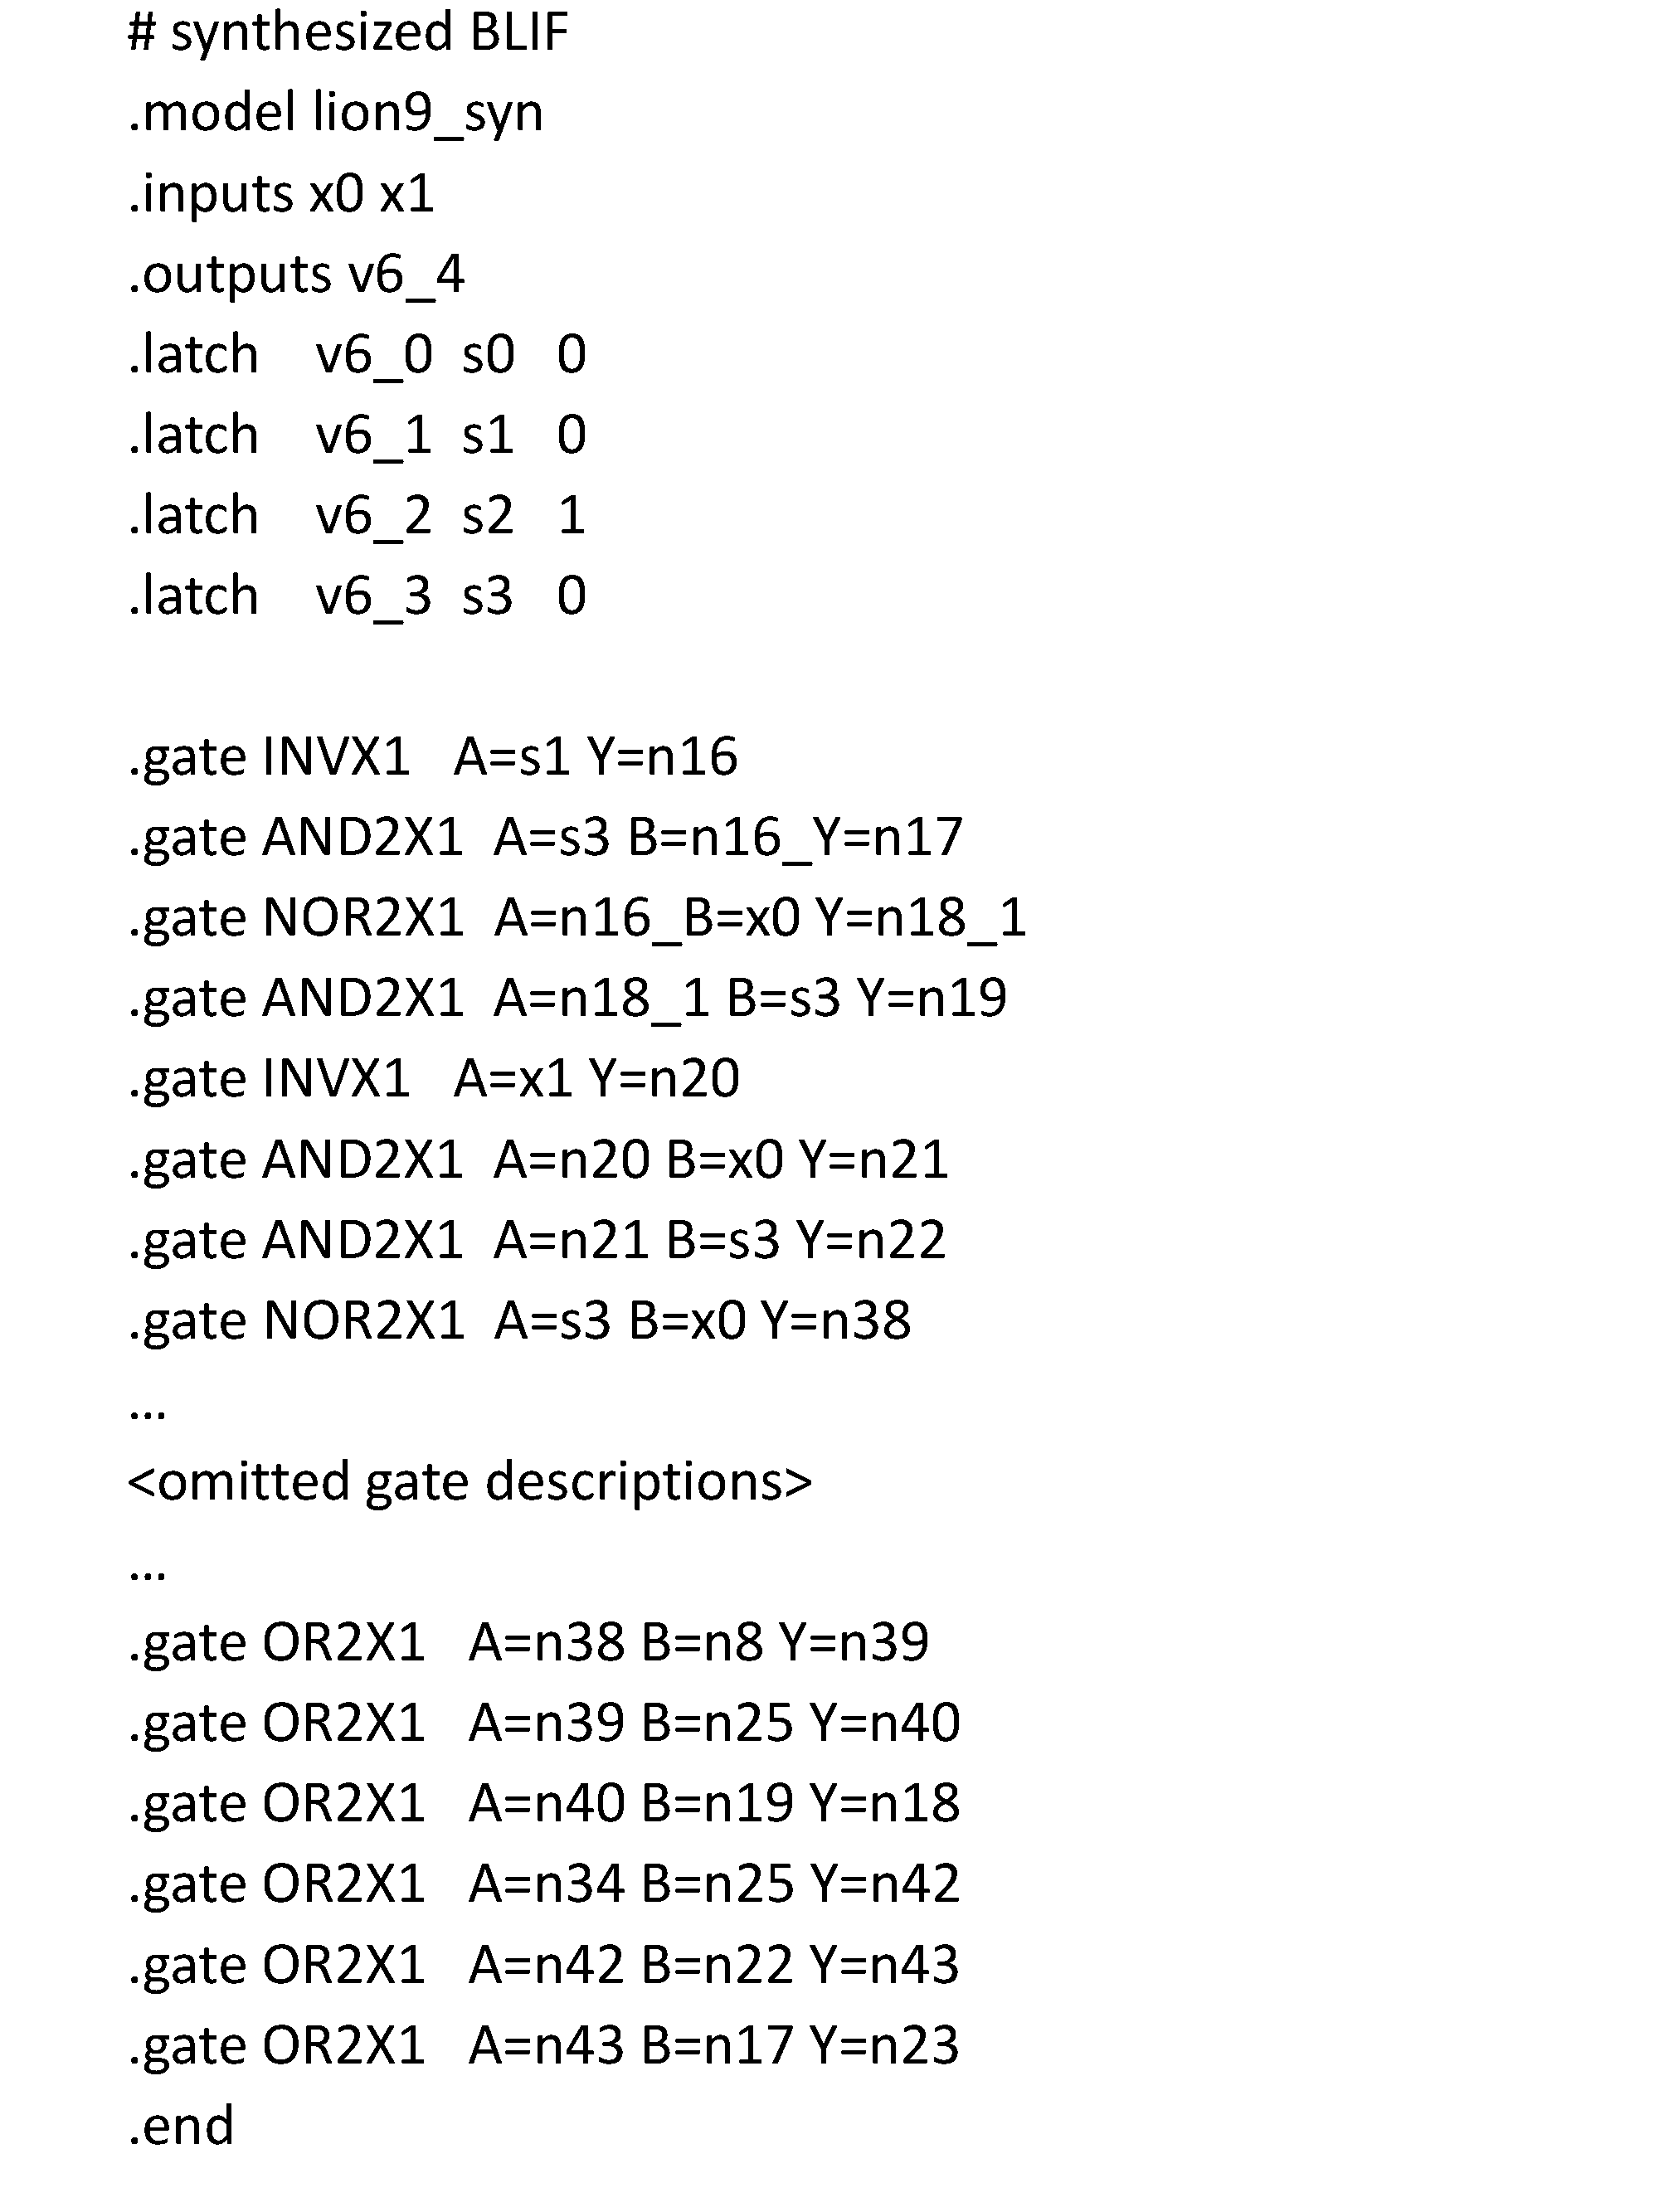
\includegraphics[width=\textwidth]{newfig/BLIF_syn.pdf}
% \caption{Synthesized BLIF file}
% \label{fig:BLIF_syn}}
% \end{figure}

Using our interpreter, the synthesized BLIF file is translated to a polynomial file customized for our 
polynomial reduction engine. 
The input file format includes all 
variables in RATO, along with the $Spoly$ that is need to be reduced, and polynomials in $J_{ckt}$.
% 
% \begin{figure}[hbt]
% \centering{
% 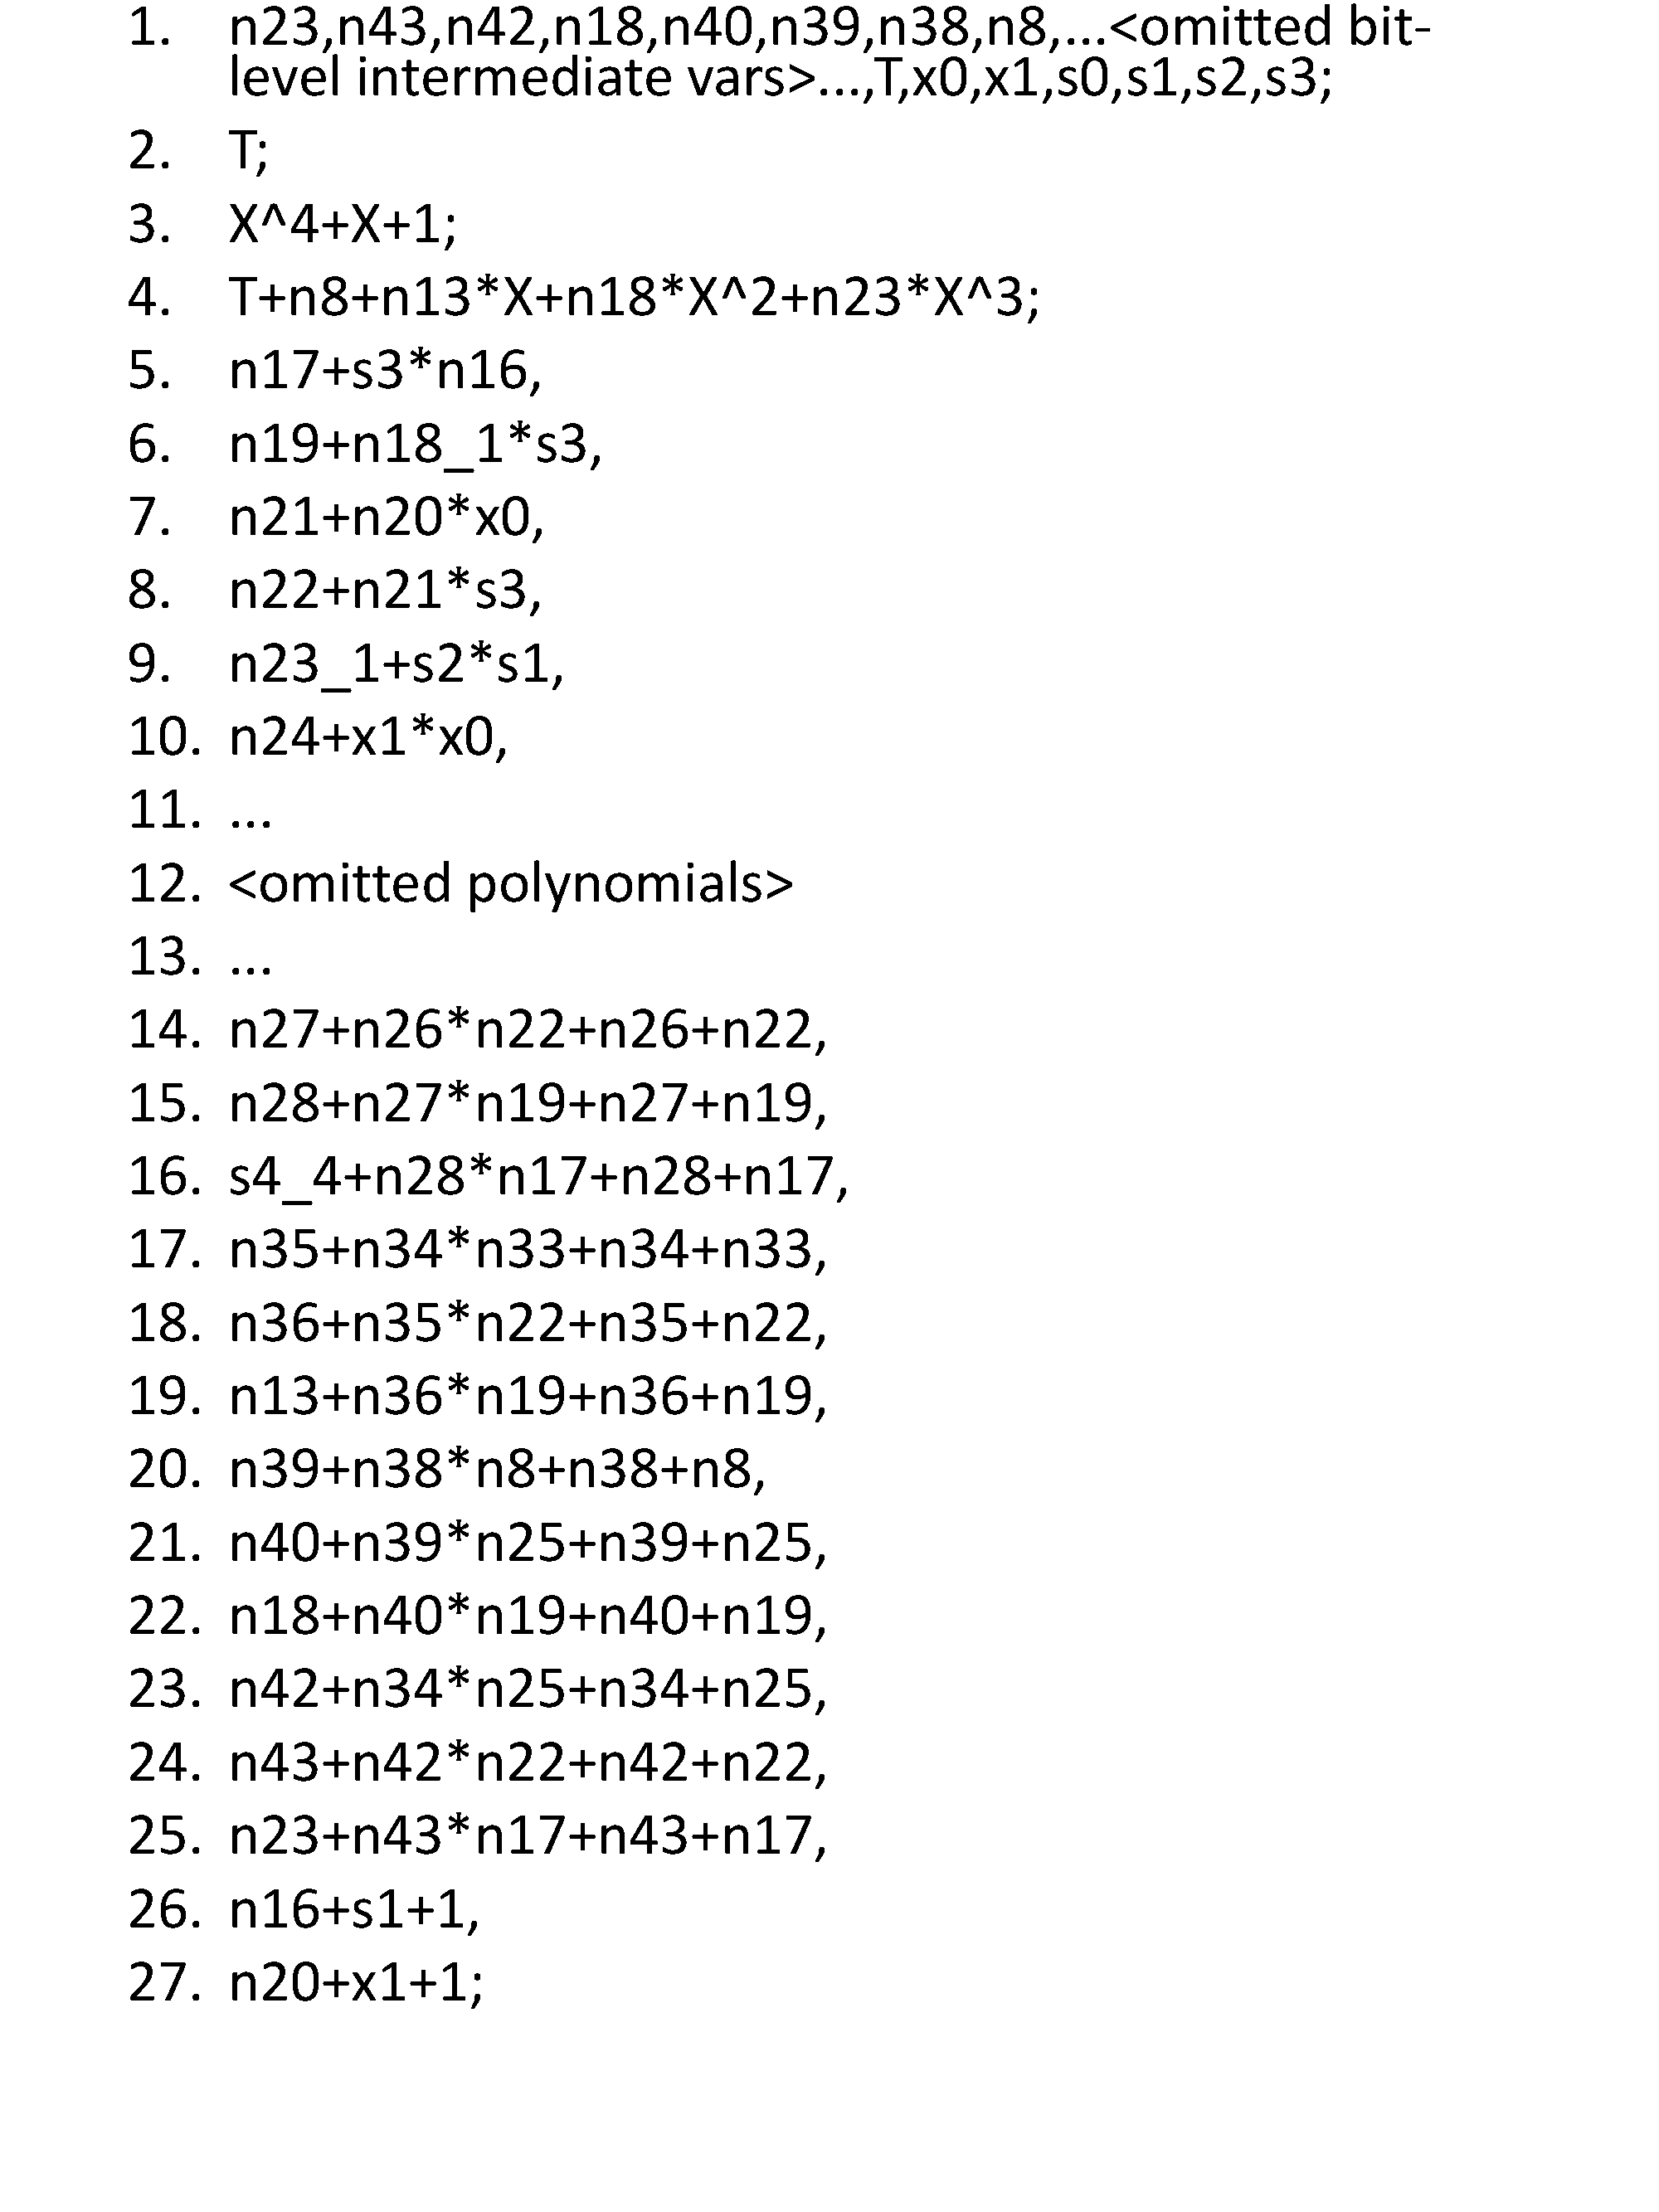
\includegraphics[width=\textwidth]{newfig/ALG.pdf}
% \caption{Polynomial file prepared for polynomial reduction engine}
% \label{fig:ALG}}
% \end{figure}

The result given by our reduction engine is in the form of the polynomial
$$T+\Func(s_0,\dots,s_{k-1},x_0,\dots,x_{n-1})$$ 
where $s_i$ and $x_j$ denote bit-level PS variables and PIs. Concretely in this example, the result is
\begin{align*}
T&+(\alpha^2+\alpha+1) x_0 x_1 s_1 s_3+(\alpha^3+\alpha) x_0 x_1 s_1+(\alpha+1) x_0 x_1 s_3 \\
&+(\alpha^3+1) x_0 s_1 s_3+(\alpha^3+\alpha) x_0 s_1 +(\alpha+1) x_0 s_3+(\alpha^2) x_0 \\
&+(\alpha^2+\alpha+1) x_1 s_1 s_3+(\alpha^3+\alpha) x_1 s_1+(\alpha^2+\alpha+1) x_1 s_3\\
&+(\alpha) x_1+(\alpha^3+1) s_1 s_3+(\alpha^3+\alpha) s_1+(\alpha^3+1) s_3+\alpha^2
\end{align*}
This is the transition function of this FSM. We utilized \textsc{Singular} to integrate both 
bit-to-word substitution and the traversal algorithm. In Figure \ref{fig:SING}, ``tran" is the transition
function we just obtained. ``init\_S" is the initial state, note it equals to ``0100" register 
reset values preloaded in the BLIF file. Moreover, 2 bits PIs $x_0,x_1$ are combined to a word-level 
PI variable $P$ using our conclusion in Example \ref{ex:PI}: ``def\_X" is the definition of 2-bit 
word, and ``red\_X" denotes the vanishing polynomial for word $P$.


After the script is executed, the traversal finishes after 4 
transition iterations, which denotes BFS depth equals to 4. According to the output in
Figure \ref{fig:Recha_result}, the final reachable states 
is a degree-9 polynomial in $T$, indicating final reachable states set contains 9 states.
And state encodings can be obtained by solving this polynomial equation.

\begin{figure}[bp]
\centering{
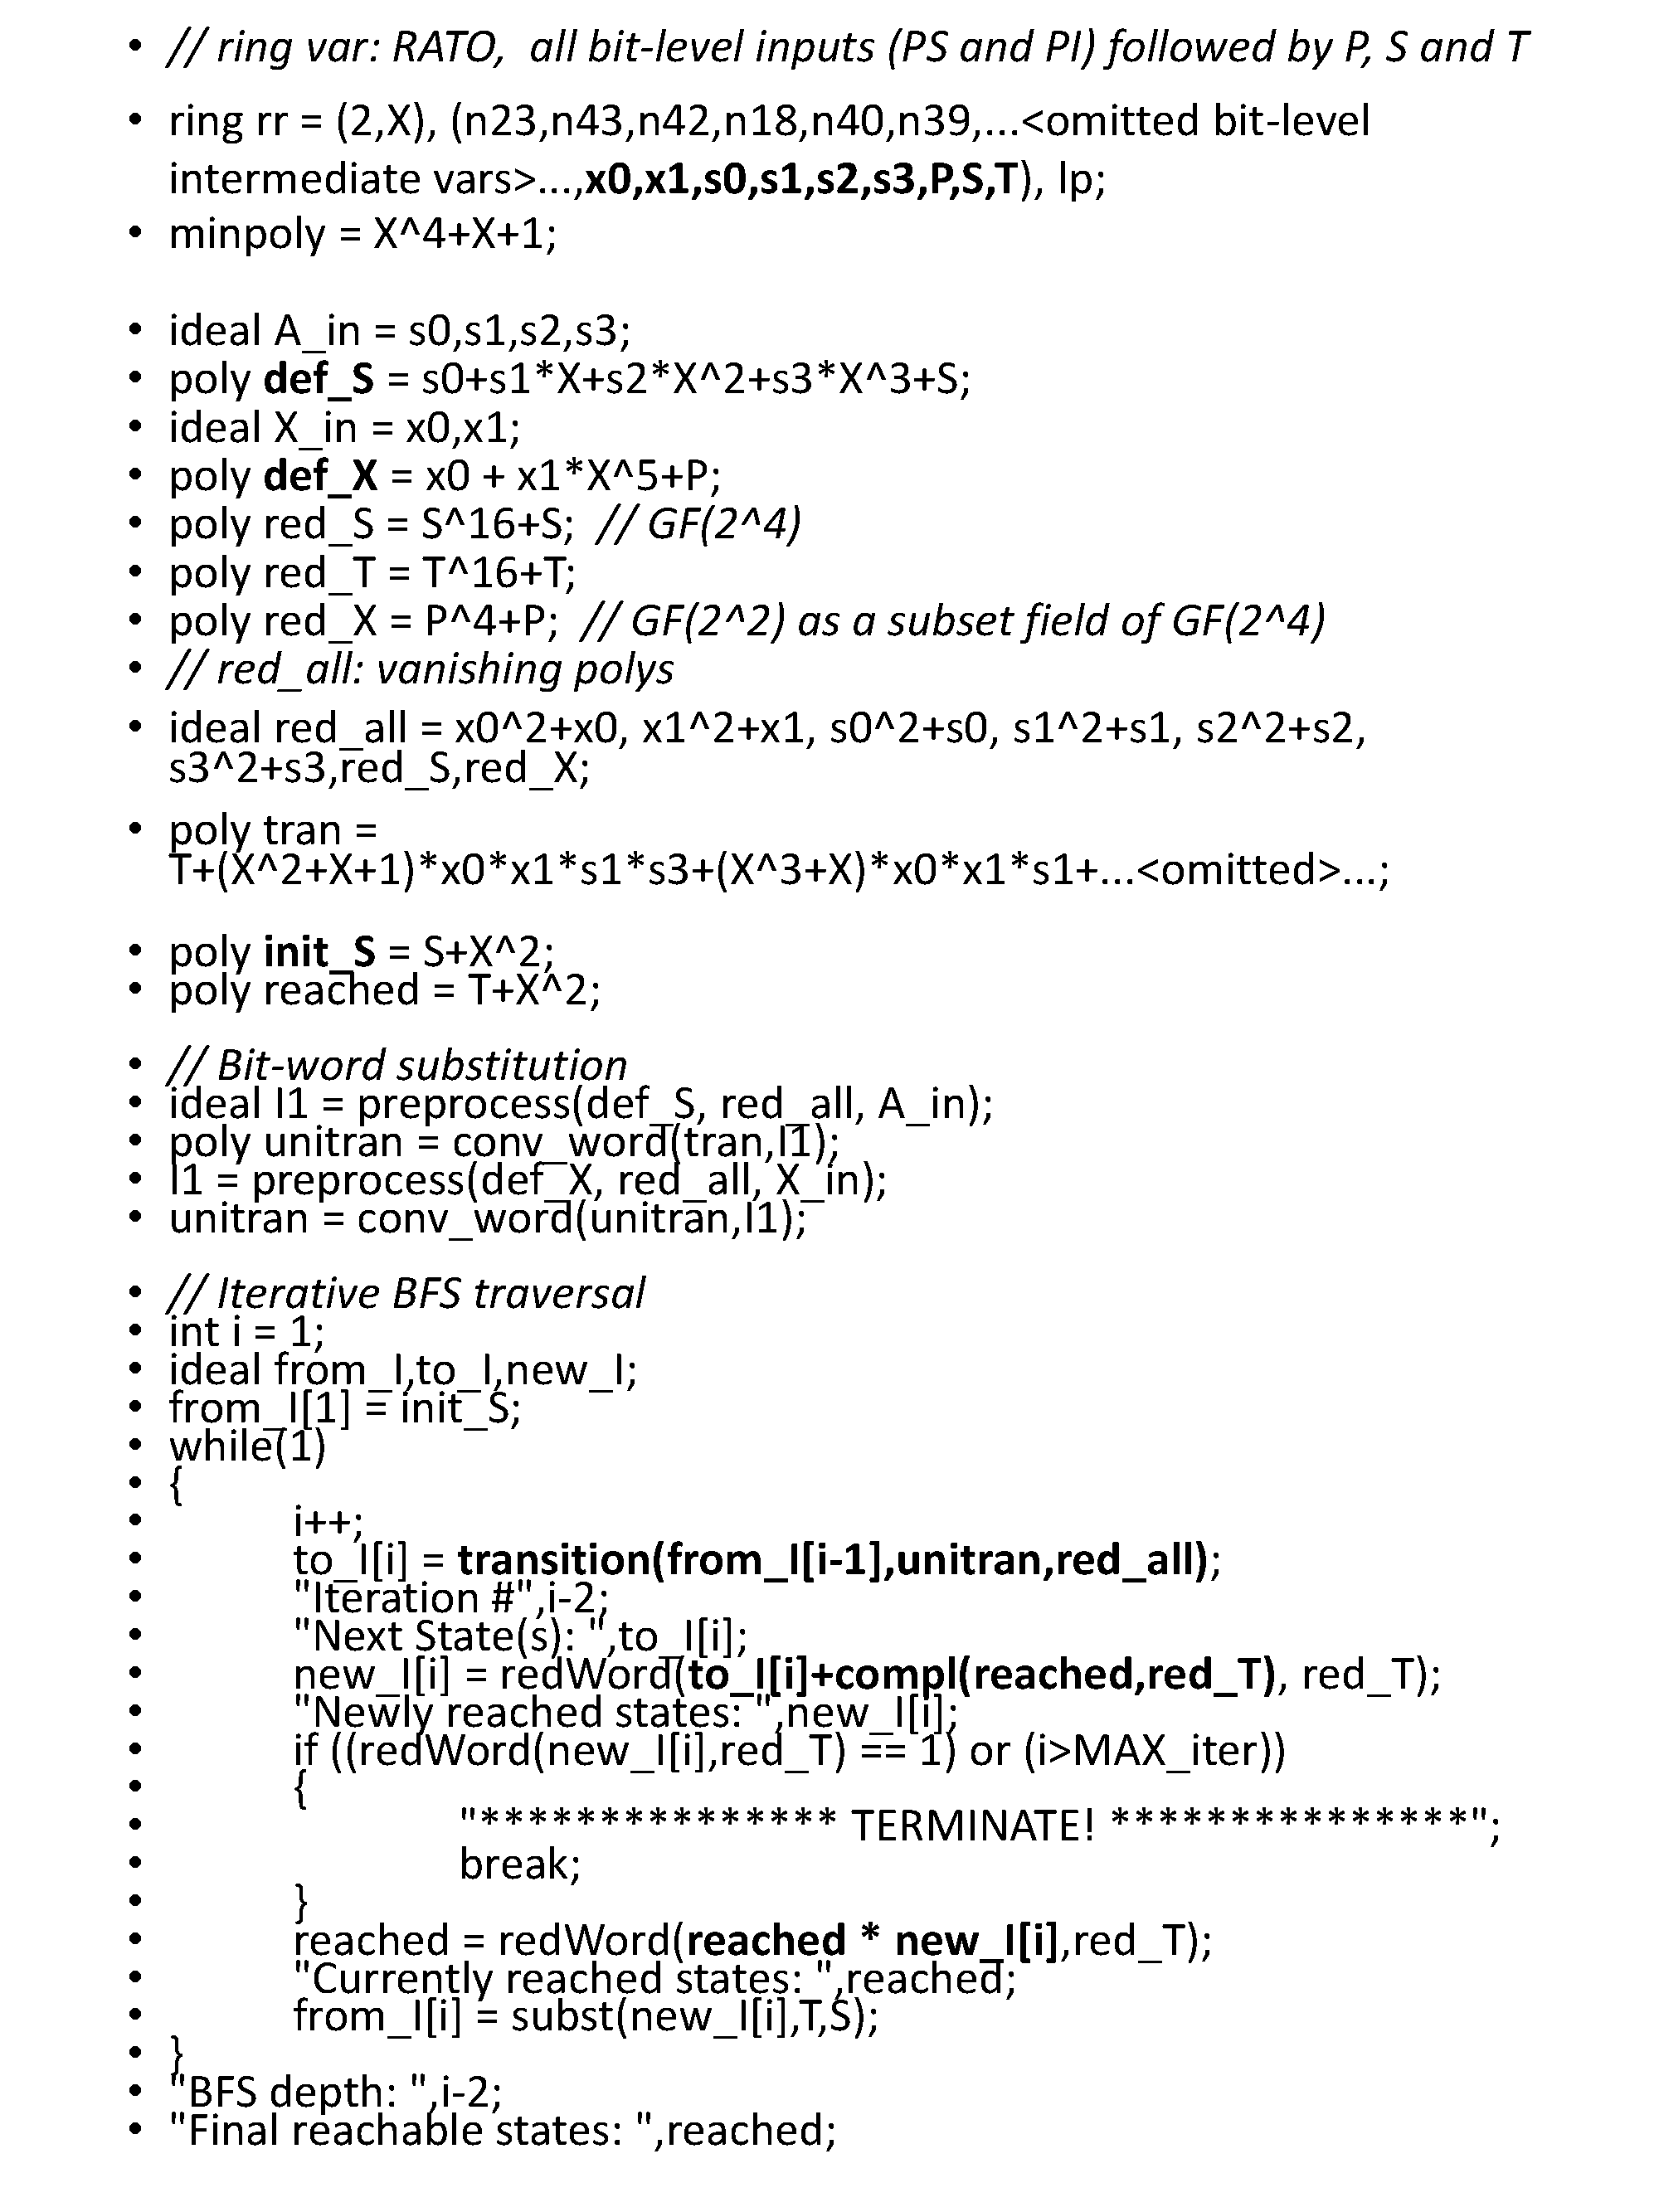
\includegraphics[width=\textwidth]{newfig/SING.pdf}
\caption{Singular script for executing bit-to-word substitution and traversal loop.}
\label{fig:SING}}
\end{figure}


\begin{figure}[bp]
\centering{
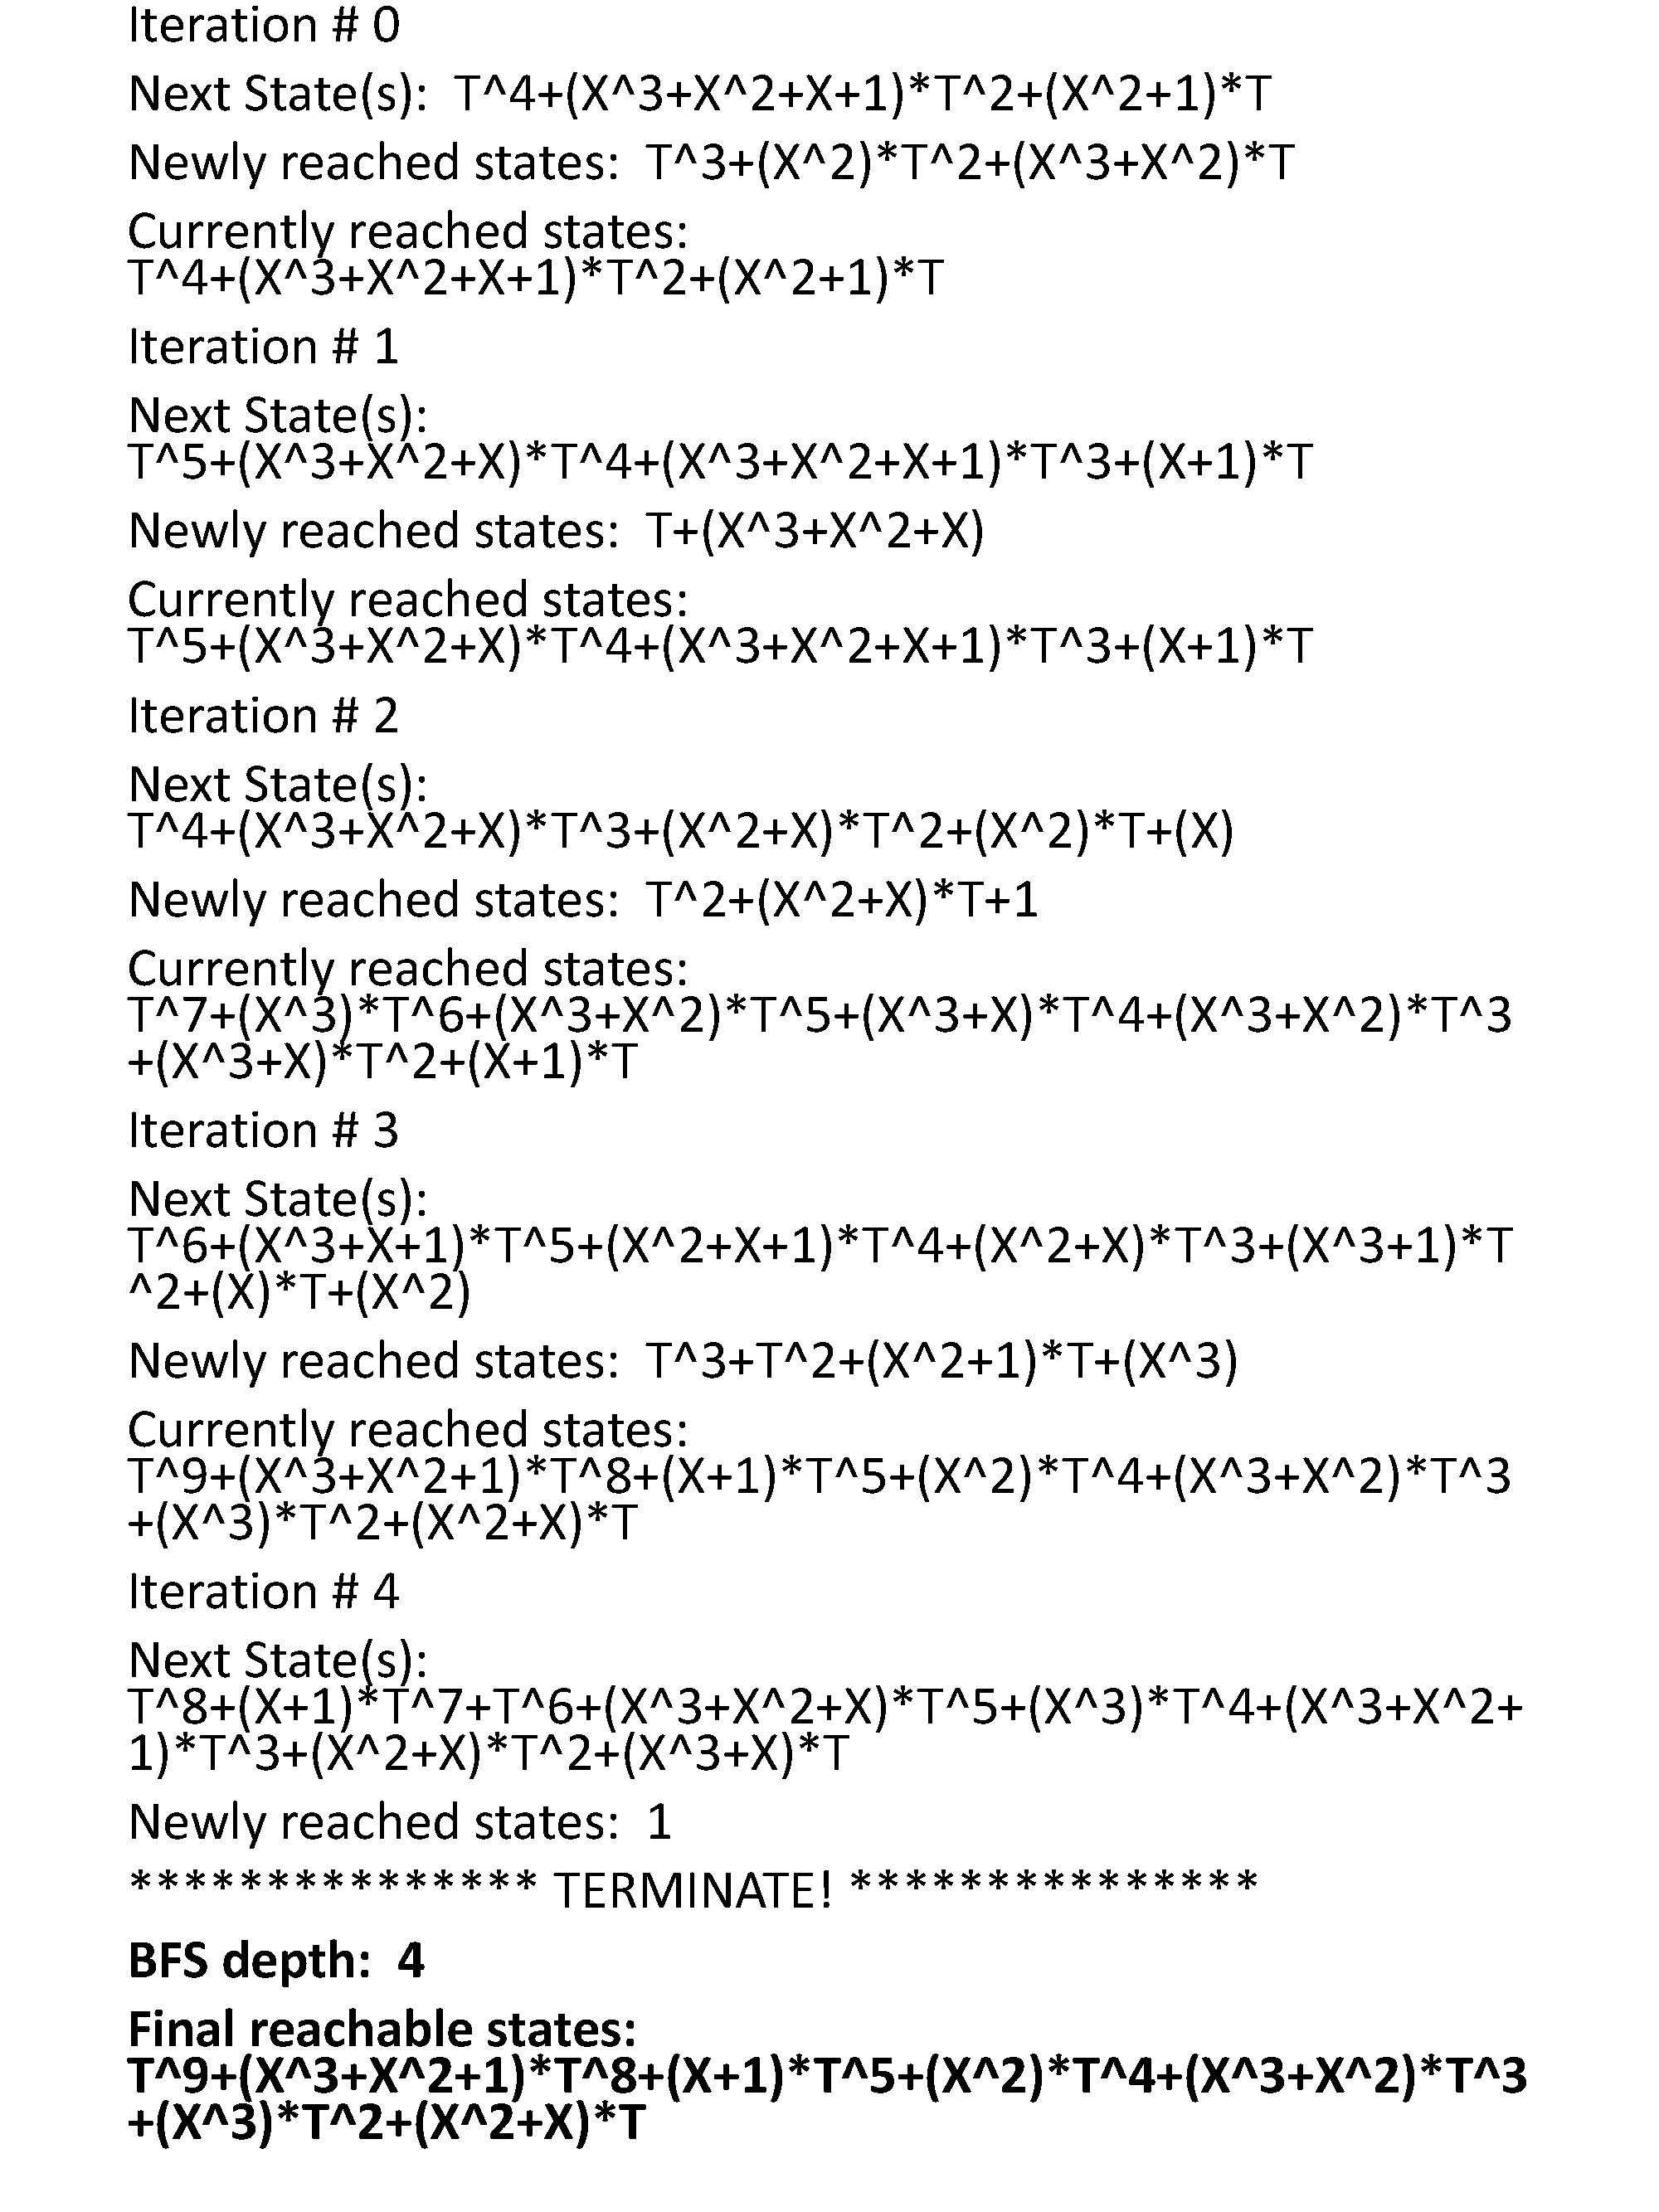
\includegraphics[width=\textwidth]{newfig/Recha_result.pdf}
\caption{The output given by our traversal tool.}
\label{fig:Recha_result}}
\end{figure}

\end{Example}

\section{Experiment Results}
\label{sec:exp_reacha}
We have implemented our traversal algorithm in 3 parts:
the first part implements polynomial reductions (division) of the
Gr\"obner basis computations, under the term order derived from the
circuit as Line 2 in Algorithm \ref{alg:refined}. This is implemented 
with our customized data structure in
C++. The second part implements the bit-level to word-level
abstraction to attain transition functions at the word-level 
%$T+\mathcal{F}(S,PIs)$ 
using the \textsc{Singular} symbolic
algebra computation system [v. 3-1-6] \cite{DGPS}, as Line 3 in 
Algorithm \ref{alg:refined}; and the third part
executes the reachability checking iterations using 
\textsc{Singular} as well. With our
tool implementation, we have performed experiments to analyze reachability
of several FSMs. Our experiments run on a desktop with
3.5GHz Intel $\text{Core}^\text{TM}$ i7-4770K Quad-core CPU, 32 GB RAM and
64-bit Ubuntu Linux OS. The experiments are shown in Table \ref{tab:recha_result}. 

There are 2 bottlenecks which restricts the performance of our tool:
one bottleneck is that the polynomial reduction engine is slow when the number of
gates (especially OR gates) is large; the other one is the high computational complexity
of Gr\"obner basis engine in general. Therefore, we pick 10 FSM
benchmarks of reasonable size for testing our tool. Among them ``b01,
b02, b06" come from ITC'99 benchmarks, %\cite{ITC99}, 
``s27, s208, s386" are from  ISCAS'89 benchmarks %\cite{yang1991logic}
 and ``bbara, beecount, dk14, donfile" are from MCNC benchmarks. %\cite{yang1991logic}.
ISCAS benchmarks are given in {\it bench} format so we can directly read gate information,
where ITC/MCNC FSMs are given in unsynthesized {\it BLIF} format so we first turn them
into gate-level netlists using AIG based synthesizer ABC. % \cite{brayton2010abc}.
Since the number of primary inputs $(m)$ is relatively small, in our experiments we partition
primary inputs as $m$ single bit-level variables. To verify the
correctness of our techniques and implementations, we compare the
number of reachable states obtained from our tool against the results
obtained from the VIS tool \cite{brayton1996vis}. 

In Table \ref{tab:recha_result}, \# States denotes the final reachable states
starting from given reset state, which given by our tool is the same with
the return value of {\it compute\_reach} in VIS. Meanwhile, from observation
of the experiment run-times, we find the reduction runtime increases
as the number of gates grows. Also, iterative reachability convergence
check's runtime reflects both the size of present state/next state
words ($k$) and the number of final reached states, which corresponds
to the degree of polynomial {\it reached} in Algorithm \ref{alg:univa}. 
Although the efficiency of our initial implementation fails to compete
with the BDD based FSM analyzer VIS, the experiment
demonstrates the power of abstraction of algebraic geometry techniques
for reachability analysis applications. 
% Currently, we are investigating techniques that
% can help us overcome the complexity of the GB computation with elimination
% orders and speed-up our approach. 

\begin{table}[tbp]
\centering
\caption{Results of running benchmarks using our tool. 
\small{Parts I to III denote the time taken by polynomial divisions,
  bit-level to word-level abstraction and iterative reachability
  convergence checking part of our approach, respectively.}}
{\small 
\begin{tabular}{|c||c|c|c|c|c|c|c|c|c|}
\hline
\multirow{3}{*}{\centering Benchmark} 
& \multirow{3}{0.9cm}{\centering \# Gates} 
& \multirow{3}{1.1cm}{\centering \# Latches} 
& \multirow{3}{*}{\centering \# PIs}
 & \multirow{3}{0.9cm}{\centering \# States}
 & \multirow{3}{1.2cm}{\centering \# iterations}
 & \multicolumn{3}{c|}{\multirow{2}{2.0cm}{\centering Runtime (sec)}}
 & \multirow{3}{1.3cm}{\centering Runtime of VIS (sec)} \\
  & & & & & &\multicolumn{3}{c|}{}& \\
  \cline{7-9}
    & & & & & & I & II & III & \\
\hline
\hline
b01 & 39  & 5  & 2 & 18  & 5  & $<0.01$ & 0.01 & 0.02 & $<0.01$\\
b02 & 24  & 4  & 1 & 8 & 5 & $<0.01$  & 0.01 & $<0.01$ & $<0.01$ \\
b06 & 49  & 9  & 2 & 13 & 4 & $<0.01$ & 0.07 & 5.0 & $<0.01$ \\
s27 & 10 & 3 & 4 & 6 & 2 & $<0.01$ & 0.01 & 0.02  & $<0.01$  \\
s208 & 61 & 8 & 11 & 16 & 16 & $<0.01$ & 0.32 & 2.4 & $<0.01$ \\
s386 & 118 & 6 & 13 & 13  & 3 & 1.0 & 7.6 & 8.2  & $<0.01$ \\
bbara & 82 & 4 & 4 & 10 & 6 & 0.04 & 0.01 & 0.04  & $<0.01$ \\
beecount & 48  & 3  & 3 & 7  & 3  &$<0.01$ & 0.01 & 0.01 & $<0.01$ \\
dk14 & 120  & 3  & 3 & 7  & 2  & 45 & $<0.01$ & 0.08 & $<0.01$\\
donfile & 205  & 5  & 2 & 24 & 3  & 12316 & 0.02 & 1.7  & $<0.01$\\
\hline
\end{tabular}
}
\label{tab:recha_result}  
\end{table} 

\section{Concluding Remarks}
This chapter has presented a new approach to perform reachability
analysis of finite state machines at the word-level. This is achieved
by modeling the transition relations and sets of states by way of
polynomials over finite fields $\Fkk$, where $k$ represents the size
of the state register bits. Subsequently using the concepts of
elimination ideals, Gr\"obner bases, and quotients of ideals, we show
that the set of reachable states can be encoded, canonically, as the
variety of a univariate polynomial. This polynomial is computed using
the Gr\"obner basis algorithm {\it w.r.t.} an elimination term
order. Experiments are conducted with a few FSMs that validate the
concept of word-level FSM traversal using algebraic geometry. 

\chapter{Functional Verification of Sequential Normal Basis Multiplier}
\label{ch:normal}
In order to utilize our traversal algorithm, it is necessary to find out
a sort of suitable circuit benchmarks which is easy to compute its
Gr\"bner basis (GB). From the work of Lv et al. \cite{lv_dissertation},
we learn that arithmetic circuits in Galois field (GF) is
convertible to an ideal of circuit polynomials, and the 
ideal generators form a GB themselves when applying reverse topological
term order. Furthermore, according to the work of Pruss et al.
\cite{tim_dissertation}, with a limited computation complexity,
we can abstract the word-level signature of an arithmetic 
component working in GF. Thus, we consider the possibility 
of applying our traversal algorithm on sequential Galois
field circuits. In each frame, we can use the techniques 
from \cite{tim_dissertation} to abstract the word-level
signature of the combinational logic, which corresponds
to the transition function in our traversal algorithm.
As a result, we manage to find a type of sequential GF multiplier
which we can apply our traversal algorithm to actually 
verify its functional correctness.

\section{Motivation}
\label{sec:normal_motiv}
From the preliminaries (Chapter \ref{ch:prelim}) about FSMs, we learn that the
Moore machine does not rely on inputs for state transitions. 
As depicted in Figure \ref{fig:Moore}(a), a typical Moore machine implementation
consists of combinational logic component and register files, where
$r_0,\dots,r_k$ are present state (PS) variables 
standing for state inputs (SI), and $r_0',\dots,r_k'$ are next state (NS) variables standing for
state outputs (SO). Figure \ref{fig:Moore}(b) shows the state transition graph (STG) of 
a Moore machine with $k+1$ distinct states. We notice that it forms a simple chain,
with $k$ consecutive transitions the machine reaches final state $R_k$.

\begin{figure}[H]
\centering{
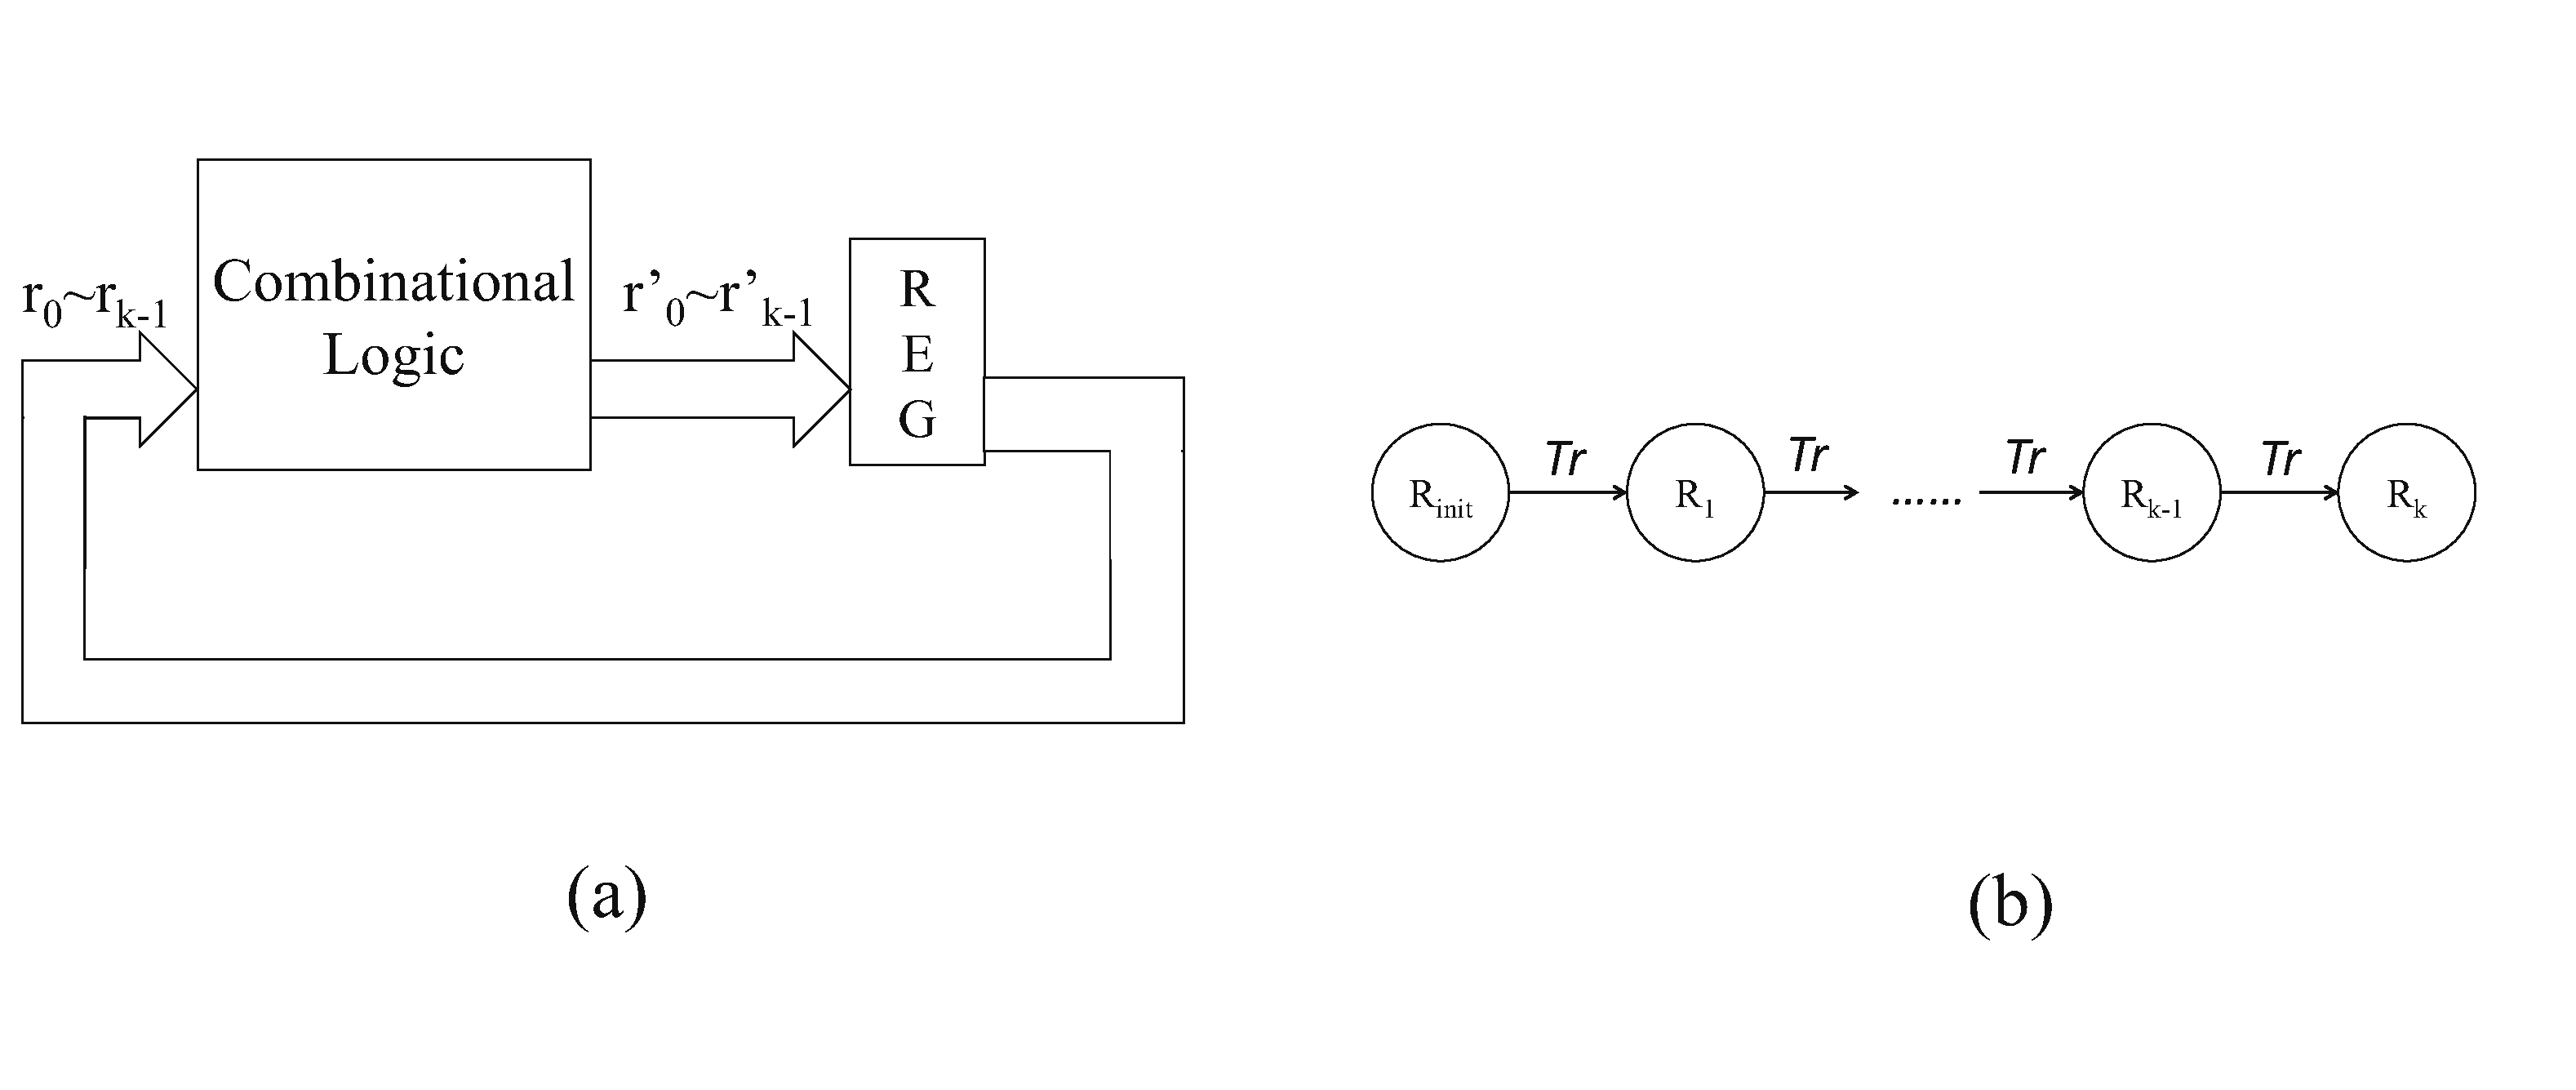
\includegraphics[width=3.5in]{newfig/Moore.eps}
\caption{A typical Moore machine and its state transition graph}
\label{fig:Moore}}
\end{figure}

In practice,
some arithmetic components are designed in sequential circuits similar to the structure in 
Figure \ref{fig:Moore}(a). Initially the operands are loaded into the registers, 
then the closed circuit executes without taking any additional information from outside,
and store the results in registers after $k$ clock cycles. Its behavior can be described using
STG in Figure \ref{fig:Moore}(b): state $R$ denotes the bits stored in registers. Concretely, $R_init$ is the initial
state (usually reset to all zeros), $R_1$ to $R_{k-1}$ are intermediate results stored as SO of current state and SI
for next state, and $R_k$ (or $R_{final}$) is the final result given by arithmetic circuits (and equals to the answer
to arithmetic function when circuit is working functional correctly).
This kind of design results in 
reusing a smaller combinational logic component such that the area cost is greatly optimized.
However, it also brings difficulties in verifying the the circuit functions.

\begin{figure}[H]
\centering{
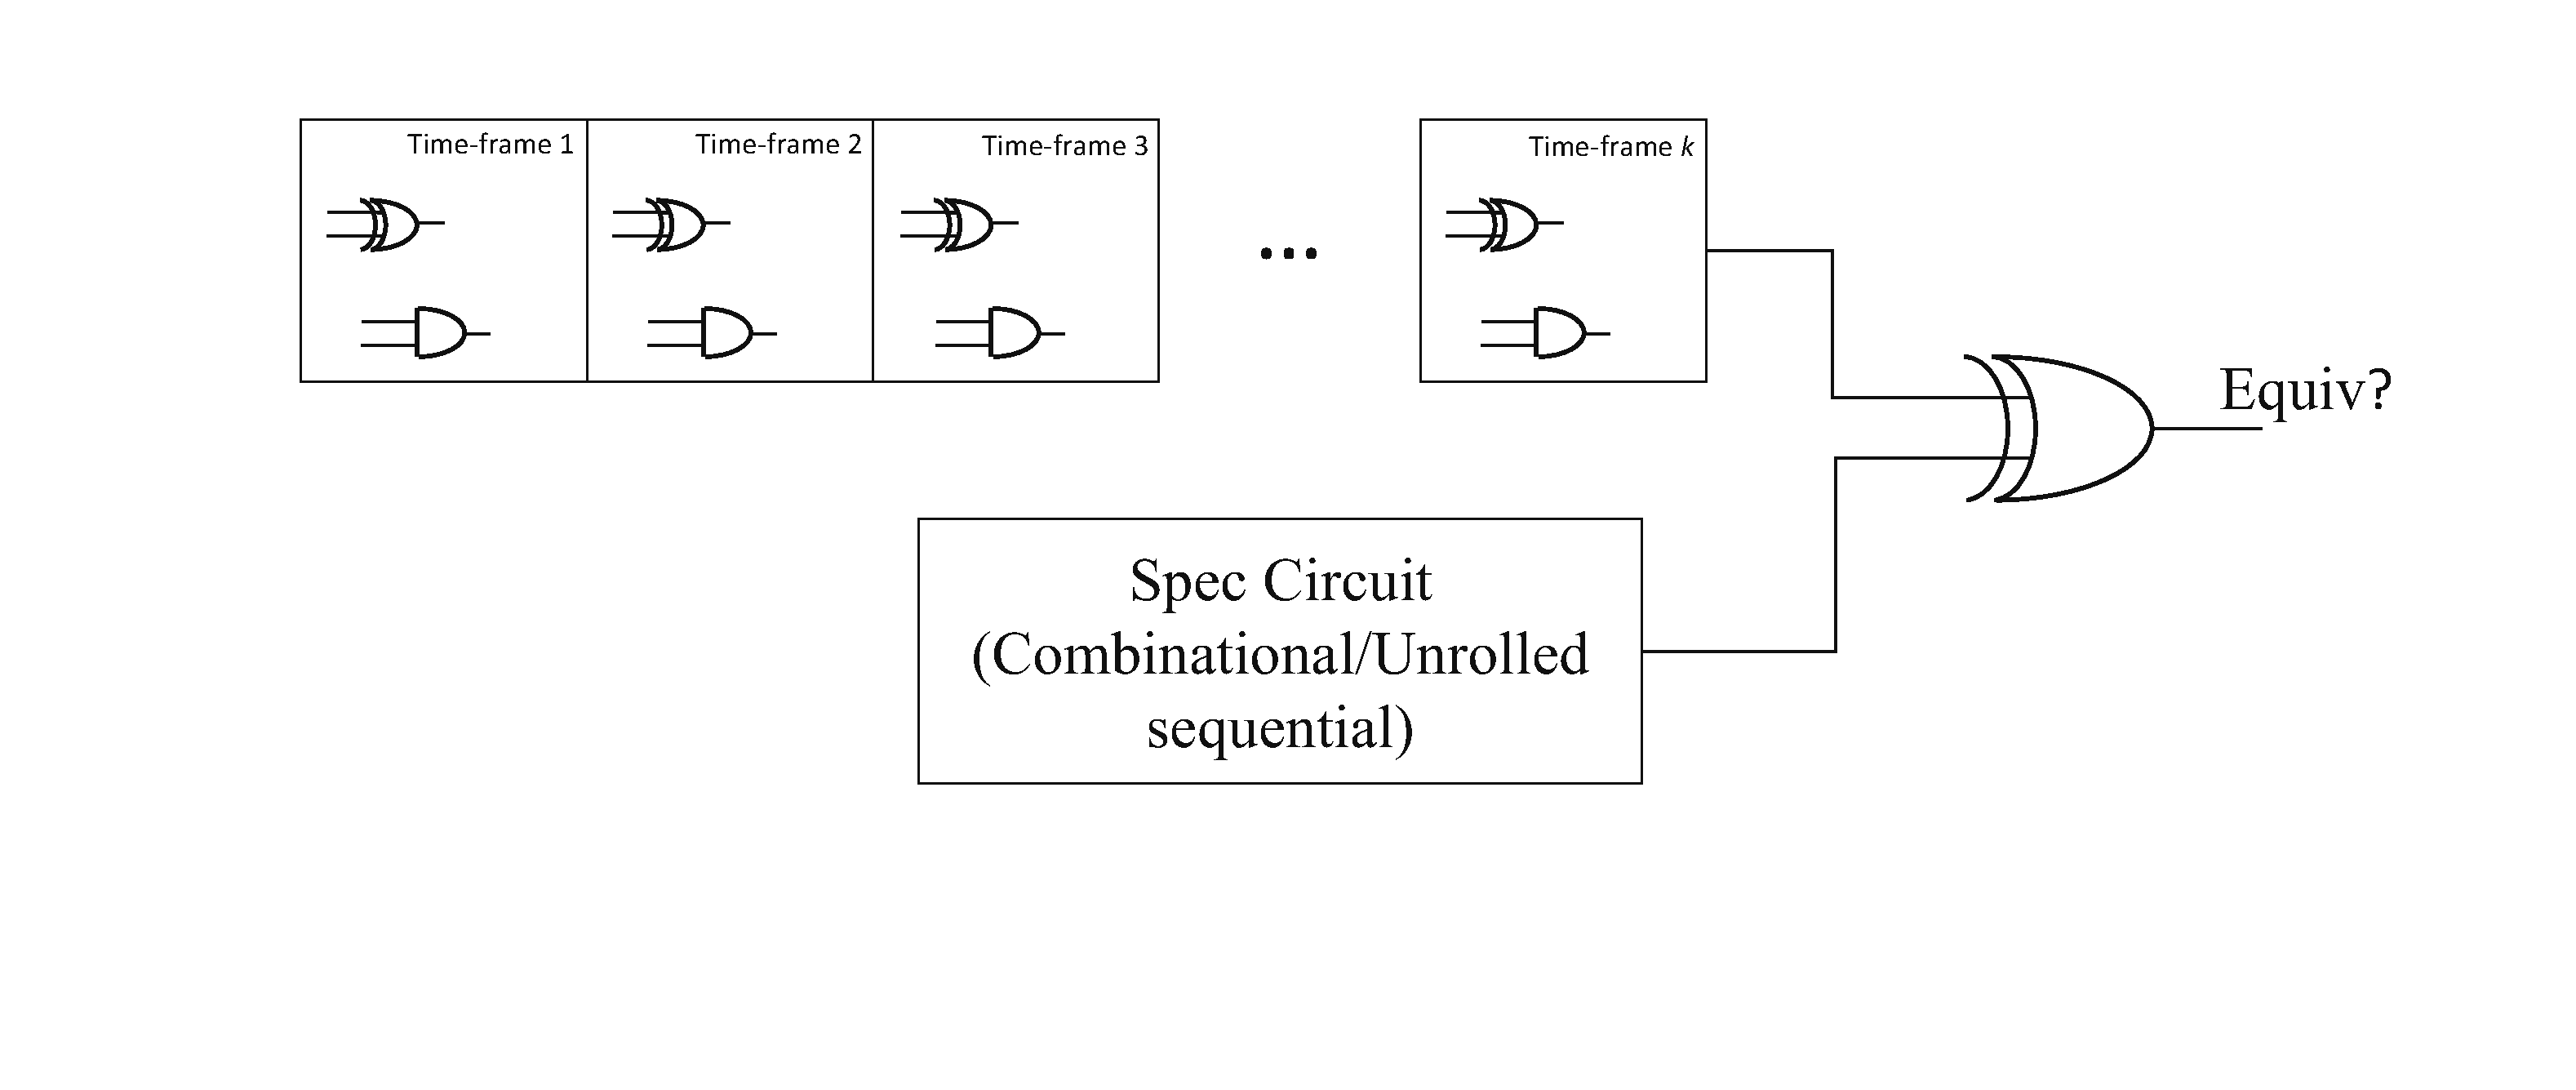
\includegraphics[width=3.5in]{newfig/convention.eps}
\caption{Conventional verification techniques based on bit-level unrolling and equivalence checking}
\label{fig:convention}}
\end{figure}

Conventional methods to such a sequential circuit may consist of unrolling the circuit for 
$k$ time-frames, and performing an equivalence checking between the unrolled machine and
the specification function. However, the number of gates will grow fast when doing unrolling
on bit-level. Meanwhile the structural similarity based equivalence checking techniques 
will fail when the sequential circuit is highly customized and optimized from the naive specification 
function. As a result, conventional techniques is grossly inefficient for large circuits.
Therefore, a new method based on our proposed word-level FSM traversal technique is worthy to be explored.

\section{Normal Basis Multiplier over Galois Field}
Given a Galois field (GF) $\Fkk$ is a finite field with  $2^k$ elements and characteristic equals to 2.
Its elements can be written in polynomials of $\alpha$, when there is an irreducible polynomial $p(\alpha)$
defined.

If we use a basis $\{1,\alpha,\alpha^2,\alpha^3,\dots,\alpha^{k-1}\}$, we can easily transform polynomial representations
to binary bit-vector representations by recording the coefficients. For example,

\begin{table}[H]
\centering
\caption{Bit-vector, Exponential and Polynomial representation of
elements in  ${\mathbb{F}}_{2^4} = {\mathbb{F}}_2[x]
\pmod{x^4+x^3+1}$}
\begin{tabular}{|c|c||c|c|} 
\hline
$a_3a_2a_1a_0$ & Polynomial     &$a_3a_2a_1a_0$ & Polynomial  \\
\hline
$0000$        & $0$           & $1000$  &$\alpha^3$\\
\hline
$0001$        & $1$           & $1001$  & $\alpha^3 + 1$\\
\hline
$0010$        &  $\alpha$       & $1010$ & $\alpha^3 + \alpha$  \\
\hline
$0011$        &  $\alpha + 1$   & $1011$ &  $\alpha^3+\alpha+1$\\
\hline
$0100$        &  $\alpha^2$     &  $1100$ &  $\alpha^3 + \alpha^2$\\
\hline
$0101$        & $\alpha^2 + 1$ & $1101$  & $\alpha^3+\alpha^2+1$\\
\hline
$0110$        &  $\alpha^2 + \alpha$ & $1110$ &  $\alpha^3+\alpha^2+\alpha$\\
\hline
$0111$        & $\alpha^2+\alpha+1$ & $1111$ & $\alpha^3+\alpha^2+\alpha+1$\\
\hline
\end{tabular}
\label{table:booltogalois}  
\end{table}

Basis $\{1,\alpha,\alpha^2,\alpha^3,\dots,\alpha^{k-1}\}$ is called {\bf standard basis} (StdB), which results in
a straightforward representation for elements, and operations of elements such as addition and subtraction.
The addition/subtraction of GF elements in StdB follows the rules of polynomial addition/subtraction
where coefficients belong to $\mathbb F_2$. In other words, using the definition of {\it exclusive or} in
Boolean algebra, element $A$ add/subtract by element $B$ in StdB is defined as
\begin{align}\label{eqn:StdB}
A+B = A-B &= (a_0,a_1,\dots,a_{k-1})_{StdB} \xor (b_0,b_1,\dots,b_{k-1})_{StdB} \nonumber\\
&=(a_0\oplus b_0, a_1\oplus b_1,\dots,a_{k-1}\oplus b_{k-1})_{StdB} 
\end{align}

Besides addition/subtraction, multiplication is also very common in arithmetic circuit design.
The multiplication of GF elements in $\Fkk$ in StdB follows the rule of polynomial multiplication.
However, it will result in $O(k^2)$ bitwise operations. In other words, if we implement GF multiplication
in bit-level logic circuit, it will contain $O(k^2)$ gates. When the datapath size $k$ is large,
the area and delay of circuit will be costly.

In order to lower down the complexity of arithmetic circuit design, Massey and Omura \cite{MasseyOmura} % ref 7 in RH paper
use a new basis to represent GF elements, which is called {\bf normal basis} (NB).
A normal basis over $\Fkk$ is written in the form of
\begin{equation*}
N.B. ~~~ \N = \{\beta,\beta^2,\beta^4,\beta^8,\dots,\beta^{2^{k-1}}\}
\end{equation*}
Respectively, a field element in NB representation is actually
\begin{align*}
A &= (a_0,a_1,\dots,a_{k-1})_{NB} \\
  &= a_0\beta+a_1\beta^2+\cdots+a_{k-1}\beta^{2^{k-1}} \\
  &= \sum_{i=0}^{k-1} a_i\beta^{2^i}
\end{align*}

According to the definition, a normal basis is a vector where the next entry is the square of the former one.
We note that the vector is cyclic, i.e. $\beta^{2^k} = \beta$ due to {\it Fermat's little theorem}.
{\bf Normal element} $\beta$ is an element from the field which is used to construct the normal basis,
and can be represent as a power of primitive element $\alpha$: 
\begin{equation*}
\beta = \alpha^t, ~~~ 1\leq t<2^k
\end{equation*}

The addition and subtraction of elements in NB representation are similar to equation \ref{eqn:StdB}.
However, what makes NB powerful is its property when doing multiplications and exponentiations.
The following lemmas and examples illustrate this fabulous property very well.
\begin{Lemma}[Square of NB]
In $\Fkk$, equation 
\begin{equation*}
(a+b)^2 = a^2 + b^2
\end{equation*}
has been proved. According to the \textbf{binomial theorem}, it can be extended to
\begin{align*}
&(b_0\beta + b_1\beta^2 + b_2\beta^4 + \dots + b_{n-1}\beta^{2^{k-1}})^2 \\
&= b_0^2\beta^2 + b_1^2\beta^4 + b_2^2\beta^8 + \dots + b_{k-1}^2\beta \\
&= b_{k-1}^2\beta + b_0\beta^2 + b_1\beta^4 + \dots + b_{k-2}\beta^{2^{k-1}}
\end{align*}
\end{Lemma}
This lemma concludes that the square of an element in NB equals to a simple right-cyclic shift of the bit-vector.
Obviously, StdB representation does not have this benefit.

\begin{Example}[Square of NB]
In GF $\mathbb F_{2^3}$ constructed by irreducible polynomial $x^3 + x + 1$, the standard basis is denoted as 
$\{ 1, \alpha, \alpha^2\}$ where $\alpha^3+\alpha+1=0$.
Let $\beta = \alpha^3$, then $\N = \{ \beta, \beta^2, \beta^4\}$ forms a normal basis. 
Write down element $E$ using both representations:
\begin{align*}
E &= (a_0,a_1,a_2)_{StdB} = (b_0,b_1,b_2)_{NB} \\
  &= a_0 + a_1\alpha + a_2\alpha^2 = b_0\beta + b_1\beta^2 + b_2\beta^4
\end{align*}
Compute the square of $E$ in StdB first:
\begin{align*}
E^2 &= a_0 + a_1\alpha^2 + a_2\alpha^4 \\
    &= a_0 + a_2\alpha + (a_1 + a_2)\alpha^2 \\
    &= (a_0,a_2,a_1+a_2)_{StdB}
\end{align*}
When it is computed in NB, we can make it very simple:
\begin{align*}
E^2 &= \overset{\xrightarrow{Cyclic~~shift}}{(b_0,b_1,b_2)}_{NB} \\
	&= (b_2,b_0,b_1)_{NB}
\end{align*}
\end{Example}

\begin{Example}
\emph{NB multiplication:} Assume there are 2 binary vectors representing 2 operands in normal
basis: $A = (a_0, a_1, \dots, a_{n-1}), B = (b_0, b_1, \dots, b_{n-1})$; similarly the product can also be written
as: $C = A*B = (c_0, c_1, \dots, c_{n-1}).$

Then the highest digit of product can be represented by a function: $c_{n-1} = f(a_0, a_1, \dots, a_{n-1}; b_0, b_1, 
\dots, b_{n-1})$. Square both side: $C^2 = A^2*B^2$, i.e. the second highest digit $c_{n-2} = f(a_{n-1}, a_0, a_1, 
\dots, a_{n-2}; b_{n-1}, b_0, b_1, \dots, b_{n-2}).$ By this method it is easy to get all digits of product $C$.
\end{Example}

\begin{Example}
\emph{$\lambda$-Matrix:} We can employ a binary $n\times n$ matrix $M$ to describe the "function"
 mentioned above: $c_{n-1} = f(A, B) = A \cdot M \cdot B^T$, $B^T$ denotes vector transposition. 
More specifically, we denote the matrix by \emph{$k$-th $\lambda$-Matrix}: $c_k = A \cdot M^{(k)} \cdot B^T$.
Then $c_{k-1} = A \cdot M^{(k-1)} \cdot B^T = rotate(A) \cdot M^{(k)} \cdot rotate(B)^T$, which means
by right and down shifting $M^{(k-1)}$ we can get $M^{(k)}$.\\
In $F_{2^3}$ constructed by $\alpha^3 + \alpha + 1$, let $\beta = \alpha^3$, $N = \{ \beta, \beta^2, \beta^4\}$ 
is a normal basis. $0$-th $\lambda$-Matrix
\begin{equation}
M^{(0)} = \left(
\begin{array} {lcr}
0 & 1 & 0\\
1 & 0 & 1\\
0 & 1 & 1
\end{array} \right).
\end{equation}
i.e.,
\begin{equation}
c_0 = (a_0\  a_1\  a_2)\left(
\begin{array} {lcr}
0 & 1 & 0\\
1 & 0 & 1\\
0 & 1 & 1
\end{array} \right)\left(
\begin{array} {lcr}
b_0\\
b_1\\
b_2
\end{array} \right).
\end{equation}
\end{Example}

$\lambda$-Matrix is defined with cross-product terms from multiplication, which is 
\begin{equation}
Product C = (\sum_{i=0}^{n-1}a_i\beta^{2^i})(\sum_{j=0}^{n-1}b_j\beta^{2^j}) = \sum_{i=0}^{n-1}\sum_{j=0}^{n-1}a_ib_j\beta^{2^i}\beta^{2^j}
\end{equation}
The expressions $\beta^{2^i}\beta^{2^j}$ are referred to as cross-product terms, and can be represented by
normal basis, i.e.
\begin{equation}
\beta^{2^i}\beta^{2^j} = \sum_{k=0}^{n-1}\lambda_{ij}^{(k)}\beta^{2^k}, \ \ \lambda_{ij}^{(k)} \in F_2.
\end{equation}
Substitution yields, result is an expression for k-th digit of product as showed in \textit{Example B.3}:
\begin{equation}
c_k = \sum_{i=0}^{n-1}\sum_{j=0}^{n-1}\lambda_{ij}^{(k)}a_ib_j
\end{equation}
$\lambda_{ij}^{(k)}$ is the entry with coordinate $(i,j)$ in $k$-th $\lambda$-Matrix.

% After fixing this, add a whole-piece StdB vs NB example, list their cost as the conclusion
\chapter{Finding Unsatisfiable Cores of a Set of Polynomials using the Gr\"obner Basis Algorithm}
\label{ch:UNSAT}
In previous chapters, we have introduced the concept of word-level abstraction and 
reachability analysis of the state-space of sequential circuits for equivalence checking.
Modern property verification techniques employ state-space abstraction using interpolants and UNSAT 
cores. In this chapter, we explore algebraic geometry analogs of UNSAT cores which can be 
applied at both bit and word-level, actually over any field.

The Boolean satisfiability (SAT) problem is the basis of 
most decidable decision problems, as well as the basis of many formal verification techniques. 
In this chapter, we discuss a special topic branching out from SAT theory. It is about a situation 
when SAT problems give negative answer, which are called unsatisfiability (UNSAT) problems. Within 
a set of constrains (e.g., clauses, formulas, or polynomials) which is unsatisfiable, sometimes 
it is worthwhile to explore the reasons for UNSAT. From the execution of the GB algorithm, 
an auxiliary structure can be obtained to help explore the reasons causing UNSAT. This chapter introduces the 
details about the motivation, mechanism, and implementation. 

\section{Motivation}
In this section, we introduce the motivation of our UNSAT core extraction research. We
start by defining an UNSAT problem, then review the previous work and applications 
to abstraction refinement. We then present the need for finding a word-level 
analog to contemporary UNSAT reasoning techniques.

\subsection{Preliminaries of SAT/UNSAT Theory}
The Boolean satisfiability (SAT) problem is a fundamental problem in computer science.
In the following part we define the terminology related to a SAT problem \cite{anaICCAD}.

\begin{Definition}
A {\bf literal} $l$ is defined as a variable $v$, or its negation $\overline{v}$. A disjunction (OR relation)
of literals forms a {\bf clause}, i.e., $c = l_1\lor l_2 \lor \cdots \lor l_k$. 
A Boolean formula can always be written as {\bf conjunctive normal form} (CNF),
which is the conjunction (AND relation) of clauses: $F = c_1\land c_2\land\cdots\land c_k$.
\end{Definition}

Using above concepts, the SAT/UNSAT problem can also be formally defined:
\begin{Definition}
A {\bf satisfiability (SAT) problem} is a decision problem that takes a CNF formula and returns
that the formula is SAT, whenever there is an assignment of variables that makes the 
formula evaluate to true. Otherwise, the formula is unsatisfiable (UNSAT).
\end{Definition}

Figure \ref{fig:SAT} shows a simple example of a SAT problem on circuit verification:
we need to verify whether subcircuit $A$ and subcircuit $B$ have the same function, so
we build a miter circuit for their outputs $X$ and $Y$, and the equivalence checking 
problem is turned into a SAT problem as follows:

\vspace{-0.7in}
\begin{center}
\begin{align*}
&\textit{Is\ subcircuit\ A\ functionally\ equivalent\ to\ subcircuit\ B?}\\
&\Longleftrightarrow
\textit{Is\ it\ true\ that\ no\ Boolean\ vector\ assignment\ to\ PIs\ a,b,c\ exists\ such\ that\ Z=1?}
\end{align*}
\end{center}

\begin{figure}[bp]
\centering{
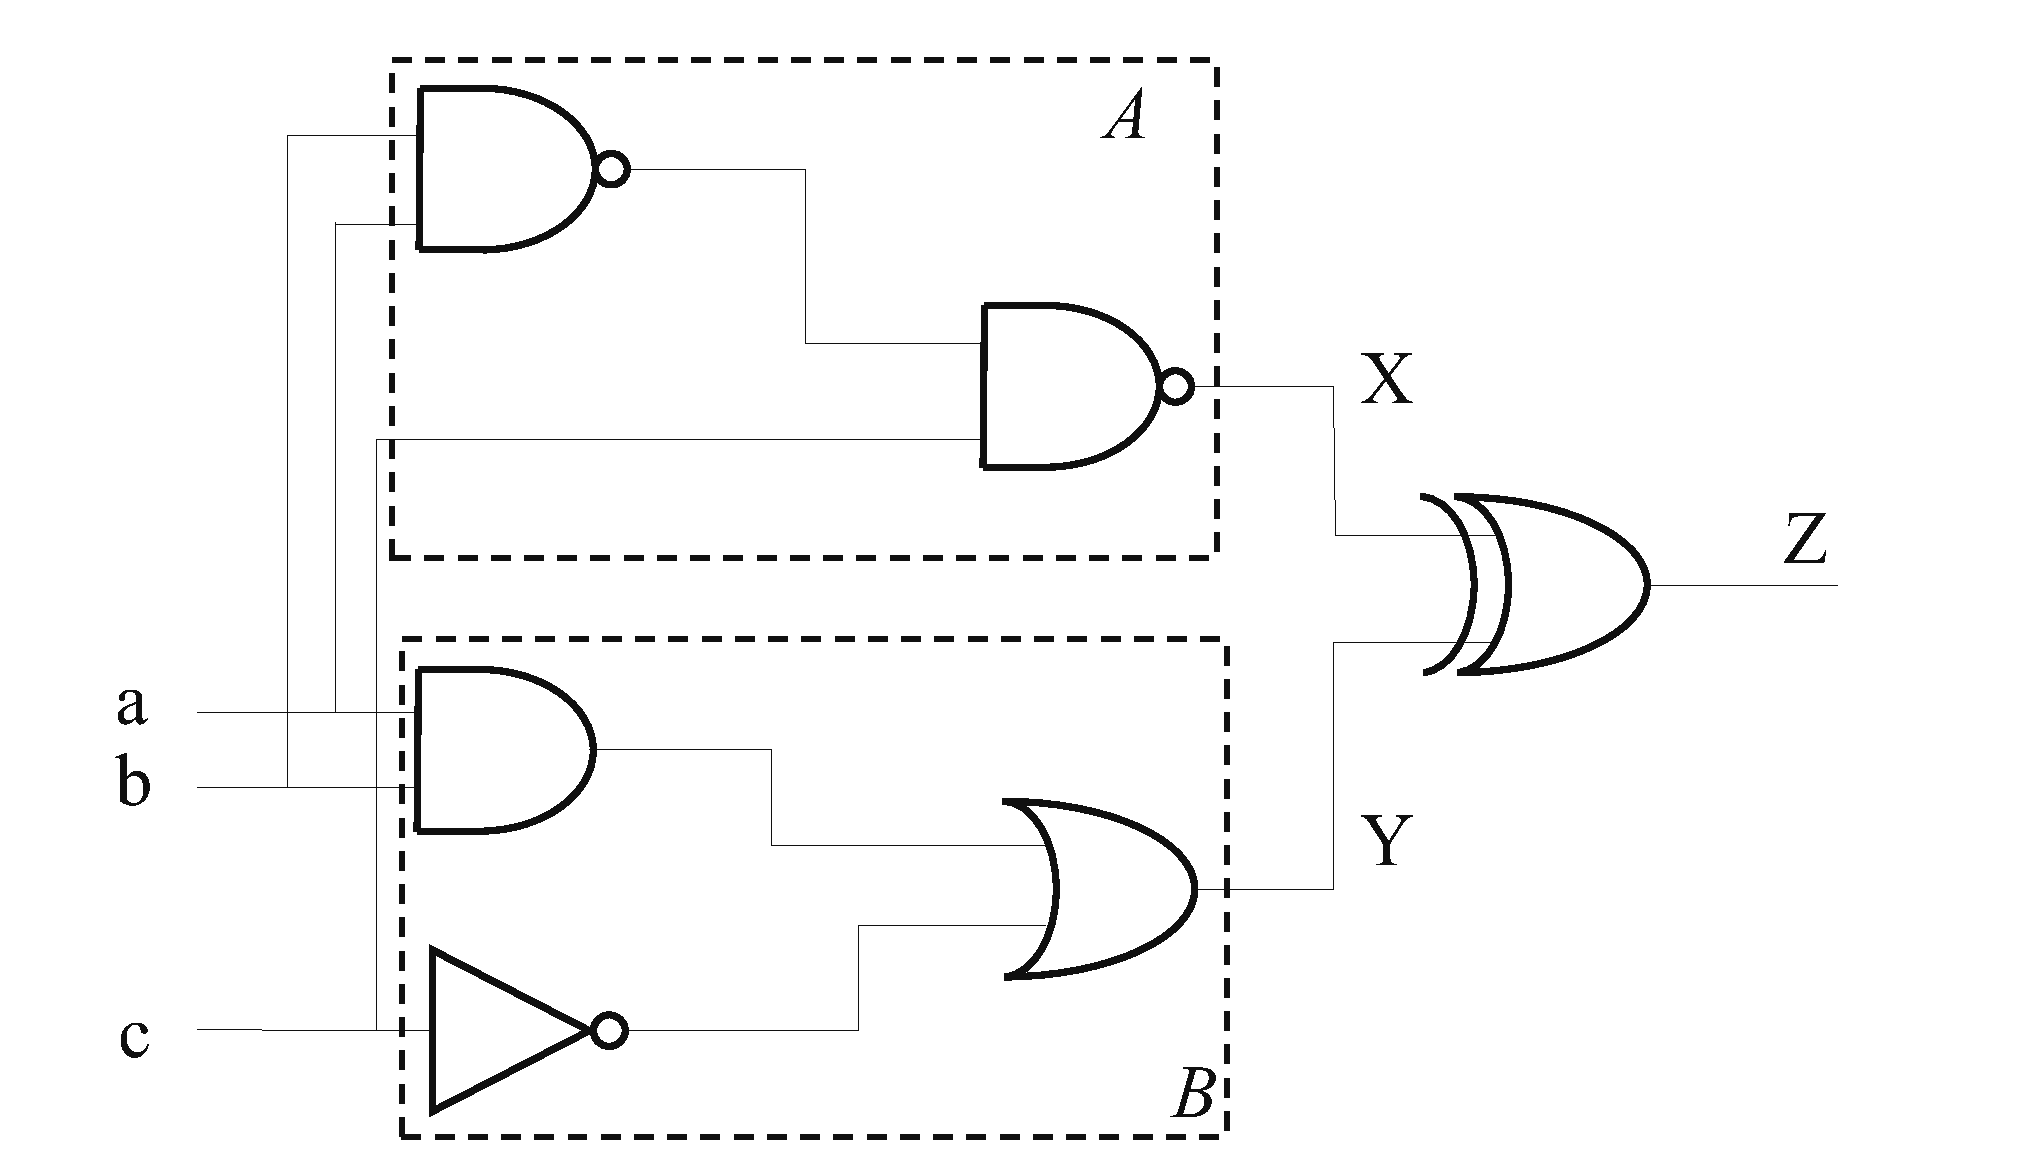
\includegraphics[scale=0.3]{newfig/fig_SAT.eps}}
\caption{An example of Boolean satisfiability problem on circuits.}
\label{fig:SAT}
\end{figure}

For an UNSAT problem, the cause of UNSAT may include a subset of clauses.
\begin{Definition}
Assume a CNF formula $F$ is UNSAT. A subformula $M \subseteq F$ is an {\bf UNSAT core} 
if $M$ is also UNSAT. Further, if $\forall c\in M$, $M\setminus\{c\}$ is SAT, then 
$M$ is called a {\bf minimal UNSAT core} of $F$.
\end{Definition}

\subsection{Previous Work on CNF-UNSAT}
In most cases, SAT problems are modeled as conjunctive normal form (CNF) formulas, and solved by procedures based on 
the Davis-Putnam and Davis-Logemann-Loveland (DPLL) algorithm. The main idea of the DPLL algorithm
is recursive branching and backtrack searching. To improve the efficiency of a DPLL-based
SAT solver, efforts are made to minimize the number of branches, accelerating unit propagation
and modifying backtrack algorithm. Recently, state-of-art SAT solvers developed a conflict-driven
clause learning (CDCL) technique to prune the search space, which is effective at reducing
search time.

When a SAT solver fails to give a SAT assignment, it will provide an {\it UNSAT proof} or {\it refutation proof}
to prove the problem is UNSAT. By analyzing clauses involved in the UNSAT proof, we can 
generate a subformula which remains UNSAT. A naive method is to collect all leaf 
clauses in an UNSAT proof as an UNSAT core. In practice, a minimal UNSAT core is more valuable.
There are mainly two kinds of methods to find minimal UNSAT cores.
One is the insertion-based method, which is achieved by adding clauses to the smallest subset 
until the subset turns to be UNSAT. The other method is the deletion-based method,
which is realized by deleting clauses from a larger subset until the subset turns to be SAT.
Recently heuristics such as clause-set refinement \cite{modelrotation} and model rotation \cite{belov2011accelerating}
have been applied as improvements on the deletion/insertion-based methods.
These methods are also expanded to satisfiability modulo theories (SMT) \cite{cimatti2007simple}.

On the other hand, researchers are seeking an alternative solution for SAT problem using a totally
different method from ``old-fashioned" DPLL algorithm. One promising option is polynomial calculus (PC),
mapping Boolean variables and connectors in CNF formulas to variables and operators in 
Galois fields as examples in Table \ref{tab:booltof4}. In this way clauses are transformed to monomials/polynomials, thus theorems and concepts in computer
algebra such as Hilbert's Nullstellensatz and Gr\"obner basis can be employed to assist finding
valid assignments or proofs of unsatisfiability. Basic concepts about PC will be formally introduced with definitions
from computer algebra.

\begin{table}[bp]
\caption{Mapping Boolean operators to functions over $\Fkk$}
\centering
\begin{tabular}{|c|c|} 
\hline
 Boolean operator & Function over $\Fkk$ \\
\hline
\hline
 $a\land b$ & $a\cdot b$ \\
\hline
 $a\oplus b$ & $a+b$ \\
\hline
 $\bar{a}$ & $1+a$ \\
\hline
 $a\lor b$ & $a+b+a\cdot b$\\
\hline
\end{tabular}
\label{tab:booltof4}  
\end{table}

The inspiration to use PC to solve SAT problems first came from \cite{ceiSTOC96}.
Using PC and its variations, researchers developed many SAT solvers \cite{STABLE,BLUEVERI,PolyBoRi}. 
Besides, researchers borrow concepts from PC and combine them with traditional DPLL and clause learning techniques
to build hybrid SAT solvers \cite{condratTACAS07,Zengler2010}.

\subsection{Exploiting UNSAT Cores for Abstraction Refinement}
The problem of finding small UNSAT cores has attracted interest for decades because of 
its applications to various verification and synthesis problems.
In solving MaxSAT problems, a small UNSAT proof provides a lower bound for the branch-and-bound searching algorithm \cite{li2009maxsat}.
It is applied to solving logic synthesis problems, such as Boolean function decomposition \cite{lee2008bi}. 
Small explanation generation in general constraint programming problems also relies on small UNSAT cores \cite{cambazard2008reformulating}.

UNSAT cores can find a wide range of applications in circuit verification as well. Many abstraction refinement techniques require 
information mining from UNSAT proofs of intermediate abstractions. 
Here we use an abstraction refinement algorithm from \cite{zhang2005design} to explain how an UNSAT proof is
utilized in such techniques.

Bounded model checking (BMC) is a model checking technique which set an upper bound to the length of all paths. 
It can be solved by solving a SAT problem. Given a model $M$, property $p$, and bound $k$, 
the $k$-BMC unrolls $M$ by $k$ clock-cycles and generates Boolean formula $F$ including violation check of $p$.
Then $F$ is fed to a SAT solver, if the SAT solver returns SAT, then $p$ is violated in 
some paths shorter than $k$. Otherwise, UNSAT indicates $p$ is not violated in all paths 
shorter than $k$. Algorithm \ref{alg:absrefine} makes an improvement on BMC using 
abstraction refinement.

% \IncMargin{1em}
\begin{algorithm}[htb]
\SetAlgoNoLine
\LinesNumbered
	\KwIn{$M$ -- original machine, $p$ -- property to check, $k$ -- \# of steps in $k$-BMC}
	\KwOut{If $p$ is violated, return error trace; otherwise $p$ is valid on $M$}
  $k = $ InitValue\;
  
  \eIf{$k$-BMC$(M,p,k)$ is \textbf{SAT}}
  {
	\Return{``Found error trace"}
  }
  {
	Extract UNSAT proof $\mathcal P$ of $k$-BMC\;
	$M' = $ \textit{ABSTRACT}$(M,\mathcal P)$\;
  }
  \eIf{MODEL-CHECK$(M',p)$ returns \textbf{PASS}}
  {
	\Return{``Passing property"}
  }
  {
	Increase bound $k$\;
	goto Line 2\;
  }
\caption {Abstraction refinement using $k$-BMC}\label{alg:absrefine}
\end{algorithm}
% \DecMargin{1em}

Assume that we are given a sequential circuit with $n$ latches as shown in Figure \ref{fig:absrefine}(a). 
This circuit can be modeled as a Mealy machine $M$ and the states $s$ can be explicitly encoded by bit-level latch variables 
$l_1,\dots,l_n$. Algorithm \ref{alg:absrefine} describes an approach to check if machine $M$ violates property $p$.
This algorithm relies on $k$-BMC technique, which works on the basis of CNF-SAT solving.
The $k$-BMC represents the initial states $I$, the transition relation $T$ and property $p$ as CNF formulas.

\begin{figure}[bp]
\centering{
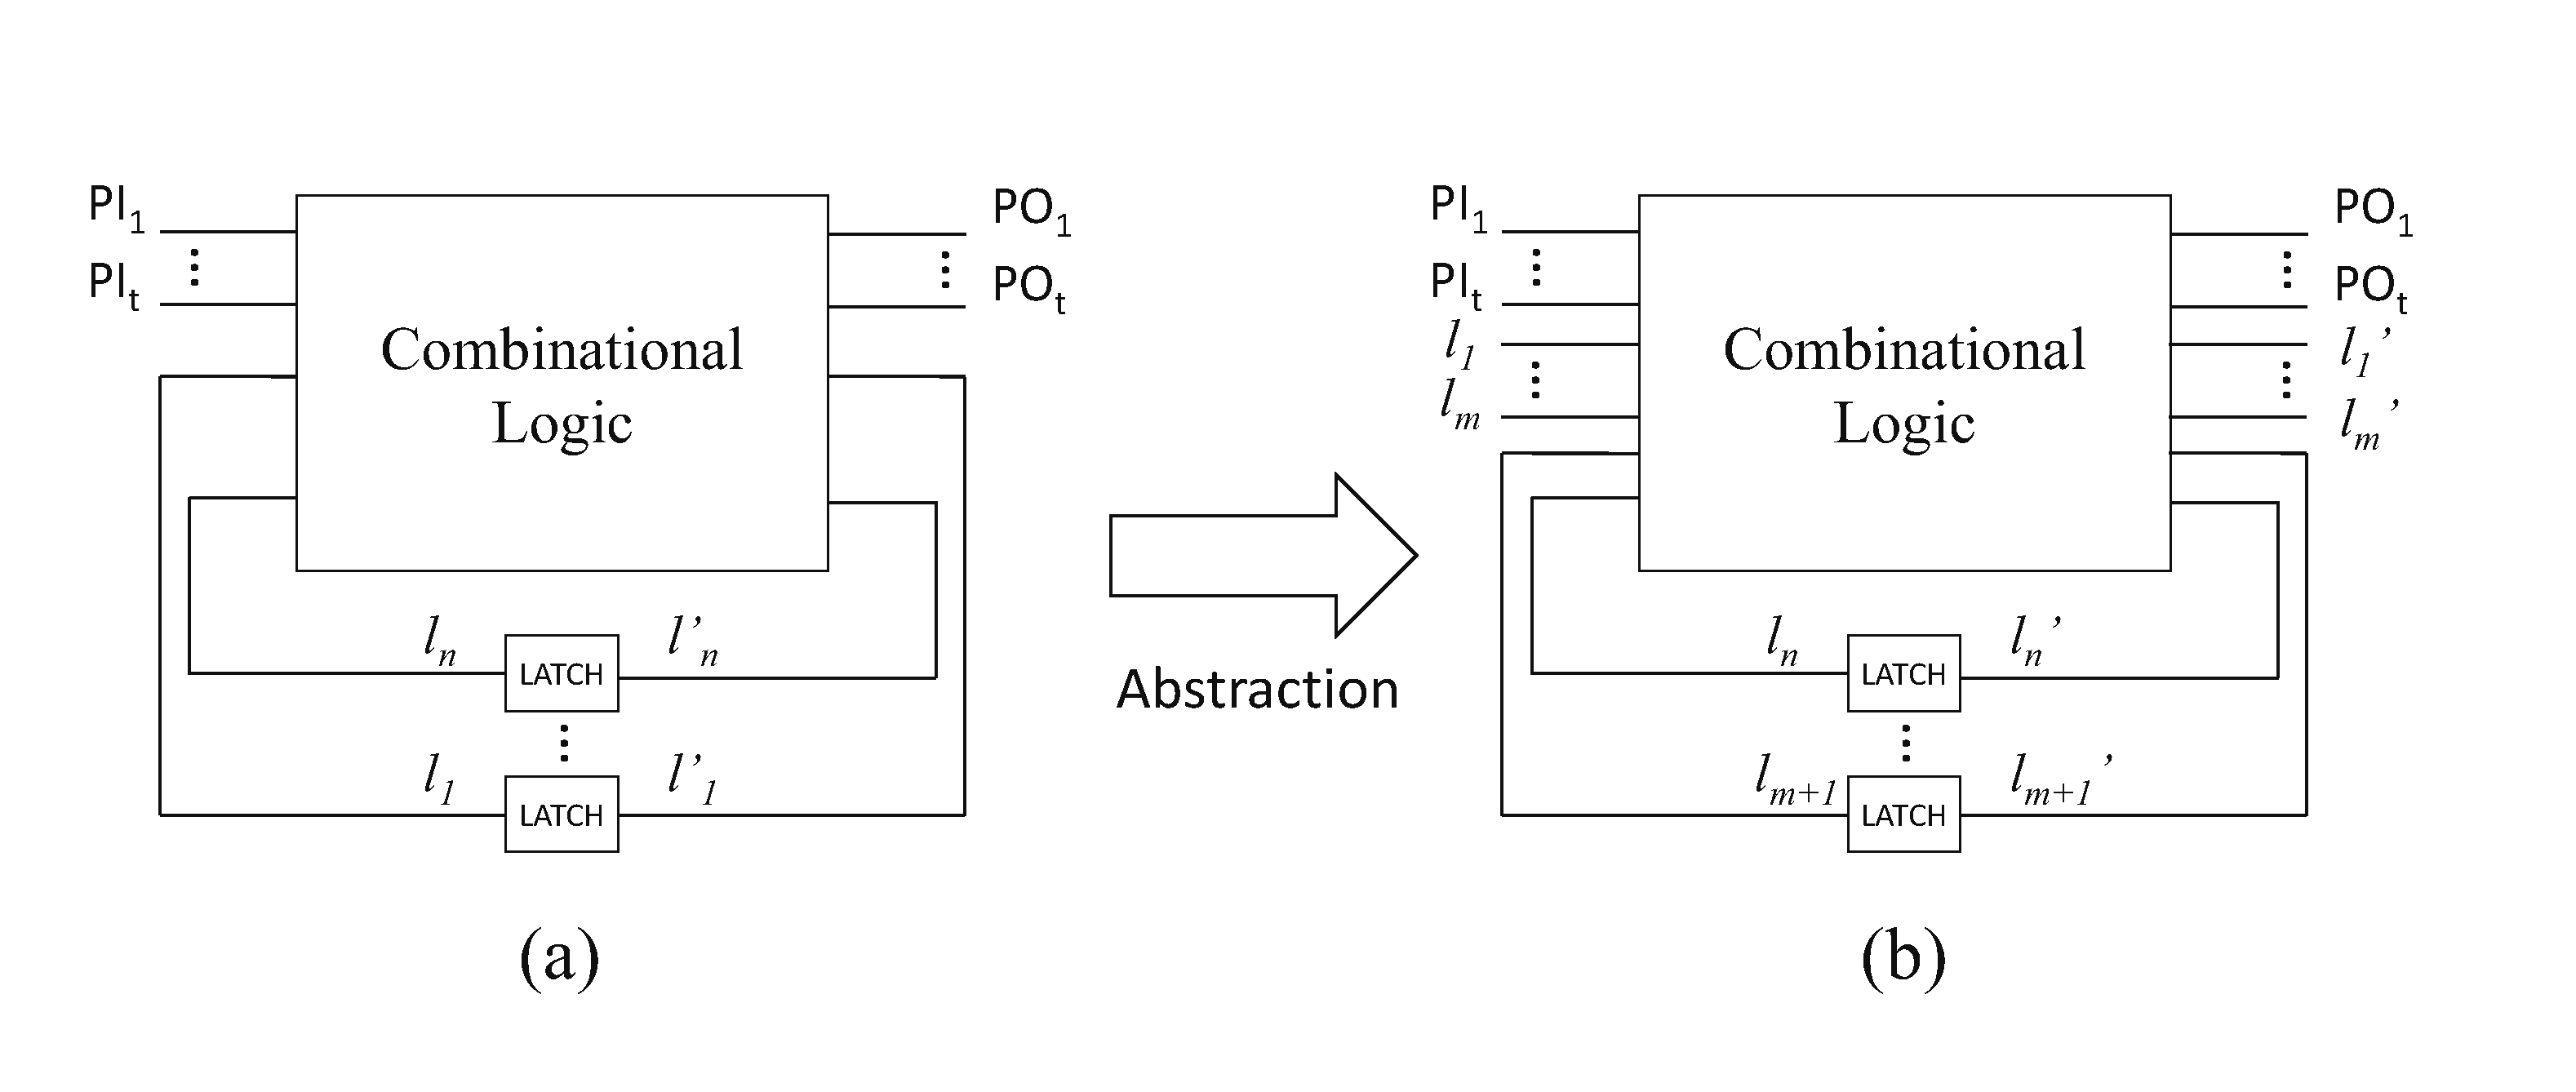
\includegraphics[width=5.5in]{newfig/refine.eps}}
\caption{Abstraction by reducing latches.}
\label{fig:absrefine}
\end{figure}

The first ``if-else" branch in Algorithm \ref{alg:absrefine} can be
explained as: we check if the conjunction of formulas 
$$I(s_0)\land \bigwedge_{i=0}^{k-1}T(s_i,s_{i+1}) \land \neg p$$
is SAT or not, where $s_i$ denotes the set of reached states in $i$-th time-frame. If the result is
SAT, then a counterexample is found that violates property $p$. If the result is UNSAT, we cannot
assert that $p$ is satisfied for the original machine $M$ because we only unrolled $M$ for a given specific number of time-frames
without any fix-point detection.
In this algorithm, we analyze the UNSAT core composed by a set of clauses whose conjunction is UNSAT.
If there are some latch variables ($L_{abs}$) not included in this UNSAT core, then we can assert that the evaluations of 
these variables will not affect the unsatisfiability of the original formula. Therefore, we can ignore them in the abstracted model.
In practice, we turn these latches into primary inputs/outputs as shown in Figure \ref{fig:absrefine}(b) ($L_{abs} = \{l_1,\dots,l_m\}$).


The second ``if-else" branch means: if we model check the abstracted machine $M'$ and find no
error trace, we can assert that property $p$ also holds on the original machine $M$. The reason for this assertion is that
the abstracted states represented using abstracted latches cover the original states, which means $M'$ is an {\bf overapproximation}
of $M$, such that 
$$(M'\implies p) \implies (M\implies p)$$ 

If we find a violation on an abstracted machine, then this
abstracted model is not a suitable model to check $p$, so we have to increase the bound $k$ to find a finer abstraction.

It is clear that UNSAT cores play an important role in abstraction refinement approaches. In \cite{zhang2005design}
the UNSAT core is extracted using a conventional CNF-SAT solver, which encounters the ``bit-blasting" problem
when the size of the datapath (number of latches in Figure \ref{fig:absrefine}) is very large. Here we propose an altogether new 
method based on Gr\"obner basis computation to extract UNSAT cores, and we believe it may become an efficient 
method according to the following observation:

% {\it Gr\"obner basis is more suitable for UNSAT problems because of following theorem:}
{\it While the complexity of computing a GB over finite fields is exponential in the number of variables,
the GB  computation is observed to be more efficient for UNSAT problems.} 
The reason is as follows:
\begin{Theorem}[Weak Nullstellensatz]
Given ideal $J\subseteq \mathbb F[x_1,\dots,x_n]$, its variety over algebraic closure $\overline{\F}$
of field $\mathbb F$ is empty if and only if its reduced Gr\"obner basis contains only one generator ``1."
$${\bf V}_{\overline{\mathbb F}}(J) = \emptyset \Longleftrightarrow \text{reduced GB}(J) = \{1\}$$
\end{Theorem}
It is well known that using Buchberger's algorithm and its variations to compute a GB has a very high space and
time complexity and is usually not practical. One reason is that the size of the GB may explode even if the term
ordering is carefully chosen. However if the reduced GB is $\{1\}$, which means every term in the original polynomials
will be canceled, the degree of remainders when computing GB with Buchberger's algorithm will be limited. 
Thus the number of polynomials in nonreduced GB is much smaller than usual.
Instead of applying polynomial calculus to SAT solving, it may be more efficient to try it for UNSAT
problems.

Moreover, conventional techniques are limited to bit-level variables (literals). Algebraic geometry methods
allow the use of word-level variables, which provides a strong potential for all applications which can be
modeled as polynomials in finite-field extensions.

\section{UNSAT Cores of Polynomial Ideals}
\label{sec:core}
In this section we provide a solution to the problem of how to use 
GB to extract the UNSAT core. 

\textbf{Problem statement: }
Let $F = \{f_1, \dots f_s\}$ be a set of multivariate polynomials in
the ring $R = \F[x_1,\dots,x_d]$ that generate ideal $J = \langle
f_1,\dots,f_s\rangle \subset R$. Suppose that it is known that $V(J) =
\emptyset$, or it is determined to be so by applying the Gr\"obner
basis algorithm. Identify a subset of polynomials $F_c \subseteq F,
J_c = \langle F_c \rangle$, such that $V(J_c) = \emptyset$
too. Borrowing the terminology from the Boolean SAT domain, we
call $F_c$ the infeasible core or the UNSAT core of $F$. 

%% Any set of polynomials $F$ with empty variety is an unsat core in
%% itself. There may be more than one unsat cores in $F$, some
%% polynomials may be common to multiple cores (i.e. the
%% cores may be non-disjoint), and these cores may have
%% different cardinalities $|F_c|$. The unsat core problems
%% are therefore further classified as: 
%% \bi
%% \item Identify a {\it minimum} core, i.e. a core of minimum
%%   cardinality. 
%% \item Identify a {\it minimal} core. An unsat core $F_{c}$ is minimal
%%   with respect to the property that while the variety of $F_{c}$ is
%%   empty, the variety of {\it any} subset of $F_c$ is {\it non-empty},
%%   i.e. $V( F_{c} - \{f_i\} ) \neq \emptyset$ for any $f_i \in
%%   F_c$. 
%% \item Identify any unsat core disregarding minimality; i.e. find any
%%   subset $F_c$ of $F$.
%% \ei

%% Let us first consider the problem of finding any $F_c \subset F$,
%% disregarding minimality. 
It is not hard to figure out that an UNSAT core should be identifiable
using the Gr\"obner basis algorithm: Assume that $F_c=F-\{f_j\}$. If
$GB(F) = GB(F_c) = \{1\}$, then it implies that $f_j$ is a member of
the ideal generated by $(F - \{f_j\})$, i.e., $f_j \in \langle F -
\{f_j\}\rangle$. Thus $f_j$ can be composed of the other
polynomials of $F_c$, so $f_j$ is  not a part of the UNSAT core, and
it can be safely discarded from $F_c$. This can be identified by means
of the GB algorithm for this ideal membership test.% (Definition \ref{def:gb}(ii)).  

A naive way (and inefficient way) to identify {\it a minimal core}
using the GB computation is as follows:
Select a polynomial $f_i$ and see if $V(F_c - \{f_i\}) = \emptyset$
(i.e., if reduced $GB(F_c - \{f_i\}) = \{1\}$). If so, discard $f_i$
from the core; otherwise retain $f_i$ in $F_c$. Select a different
$f_i$ and continue until all polynomials $f_i$ are visited for
inclusion in $F_c$. This approach will produce a minimal core, as we
would have tested each polynomial $f_i$ for inclusion in the
core. This requires $O(|F|)$ calls to the GB engine, which is really
impractical.   

\subsection{An Example Motivating Our Approach}

Buchberger's algorithm picks pairs of polynomials from a given set, computes their $Spoly$, then reduces this $Spoly$
with the given set of polynomials. If the remainder is nonzero,
it is added to the set of polynomials.
By tracking $Spoly$ computations and multivariate divisions that lead to remainder 
1, we can obtain an UNSAT core. Moreover, we can identify a minimal UNSAT core with one-time
 execution of Buchberger's algorithm.

\begin{Example}
A SAT problem is described with 8 CNF clauses:

\begin{minipage}[h]{0.3\textwidth}
\begin{align*}
&c_1: \bar{a}\lor\bar{b}\\
&c_2: a\lor\bar{b}\\
&c_3: \bar{a}\lor b\\
&c_4: a\lor b
\end{align*}
\end{minipage}
\begin{minipage}[h]{0.7\textwidth}
\begin{align*}
&c_5: x\lor y\\
&c_6: y\lor z\\
&c_7: b\lor \neg y\\
&c_8: a\lor x\lor \neg z
\end{align*}
\end{minipage}

\vspace{0.1in}
Using Boolean to polynomial mappings given in Table \ref{tab:booltof4}, we can transform them to a set of
polynomials $F=\{f_1,\dots,f_8\}$ over ring $\mathbb F_2[a,b,x,y,z]$:

\begin{minipage}[h]{0.4\textwidth}
\begin{align*}
&f_1:ab\\
&f_2:ab+a\\
&f_3:ab+b\\
&f_4:ab+a+b+1
\end{align*}
\end{minipage}
\begin{minipage}[h]{0.6\textwidth}
\begin{align*}
&f_5:xy+y+x+1\\
&f_6:yz+y+z+1\\
&f_7:by+y\\
&f_8:axz+az+xz+z
\end{align*}
\end{minipage}

\vspace{0.1in}
We compute its GB using Buchberger's algorithm with lexicographic term ordering $a>b>x>y>z$.
Since this problem is UNSAT, we will stop when ``1" is added to GB.
\begin{enumerate}[{1)}]
\item First we compute $Spoly(f_1,f_2)\xrightarrow{F}_{+} r_1$, remainder $r_1$ equals to $a$;
\item Update $F=F\cup r_1$;
\item Next we compute $Spoly(f_1,f_3)\xrightarrow{F}_{+} r_2$, remainder $r_2$ equals to $b$;
\item Update $F=F\cup r_2$;
\item We can use a directed acyclic graph (DAG) to represent the process to get $r_1,r_2$, as Figure \ref{fig:originUNSAT}(a) shows;
\item Then we compute $Spoly(f_1,f_4) = s_3= a+b+1$, obviously $a+b+1$ can be reduced (multivariate divided) by
$r_1$ , the intermediate remainder $r_3 = b+1$. It can be immediately divided by $r_2$, and the remainder is ``1," we
terminate the Buchberger's algorithm;
\item We draw a DAG depicting the process through which we obtain remainder ``1" as shown in Figure \ref{fig:originUNSAT}(b). 
From leaf ``1" we backtrace the graph to roots $f_1,f_2,f_3,f_4$. They constitute an UNSAT core for this problem
as these polynomials are the ``causes" of the unsatisfiability of the original set of polynomials.
\end{enumerate}
\end{Example}

\begin{figure}[tbp]
\centering{
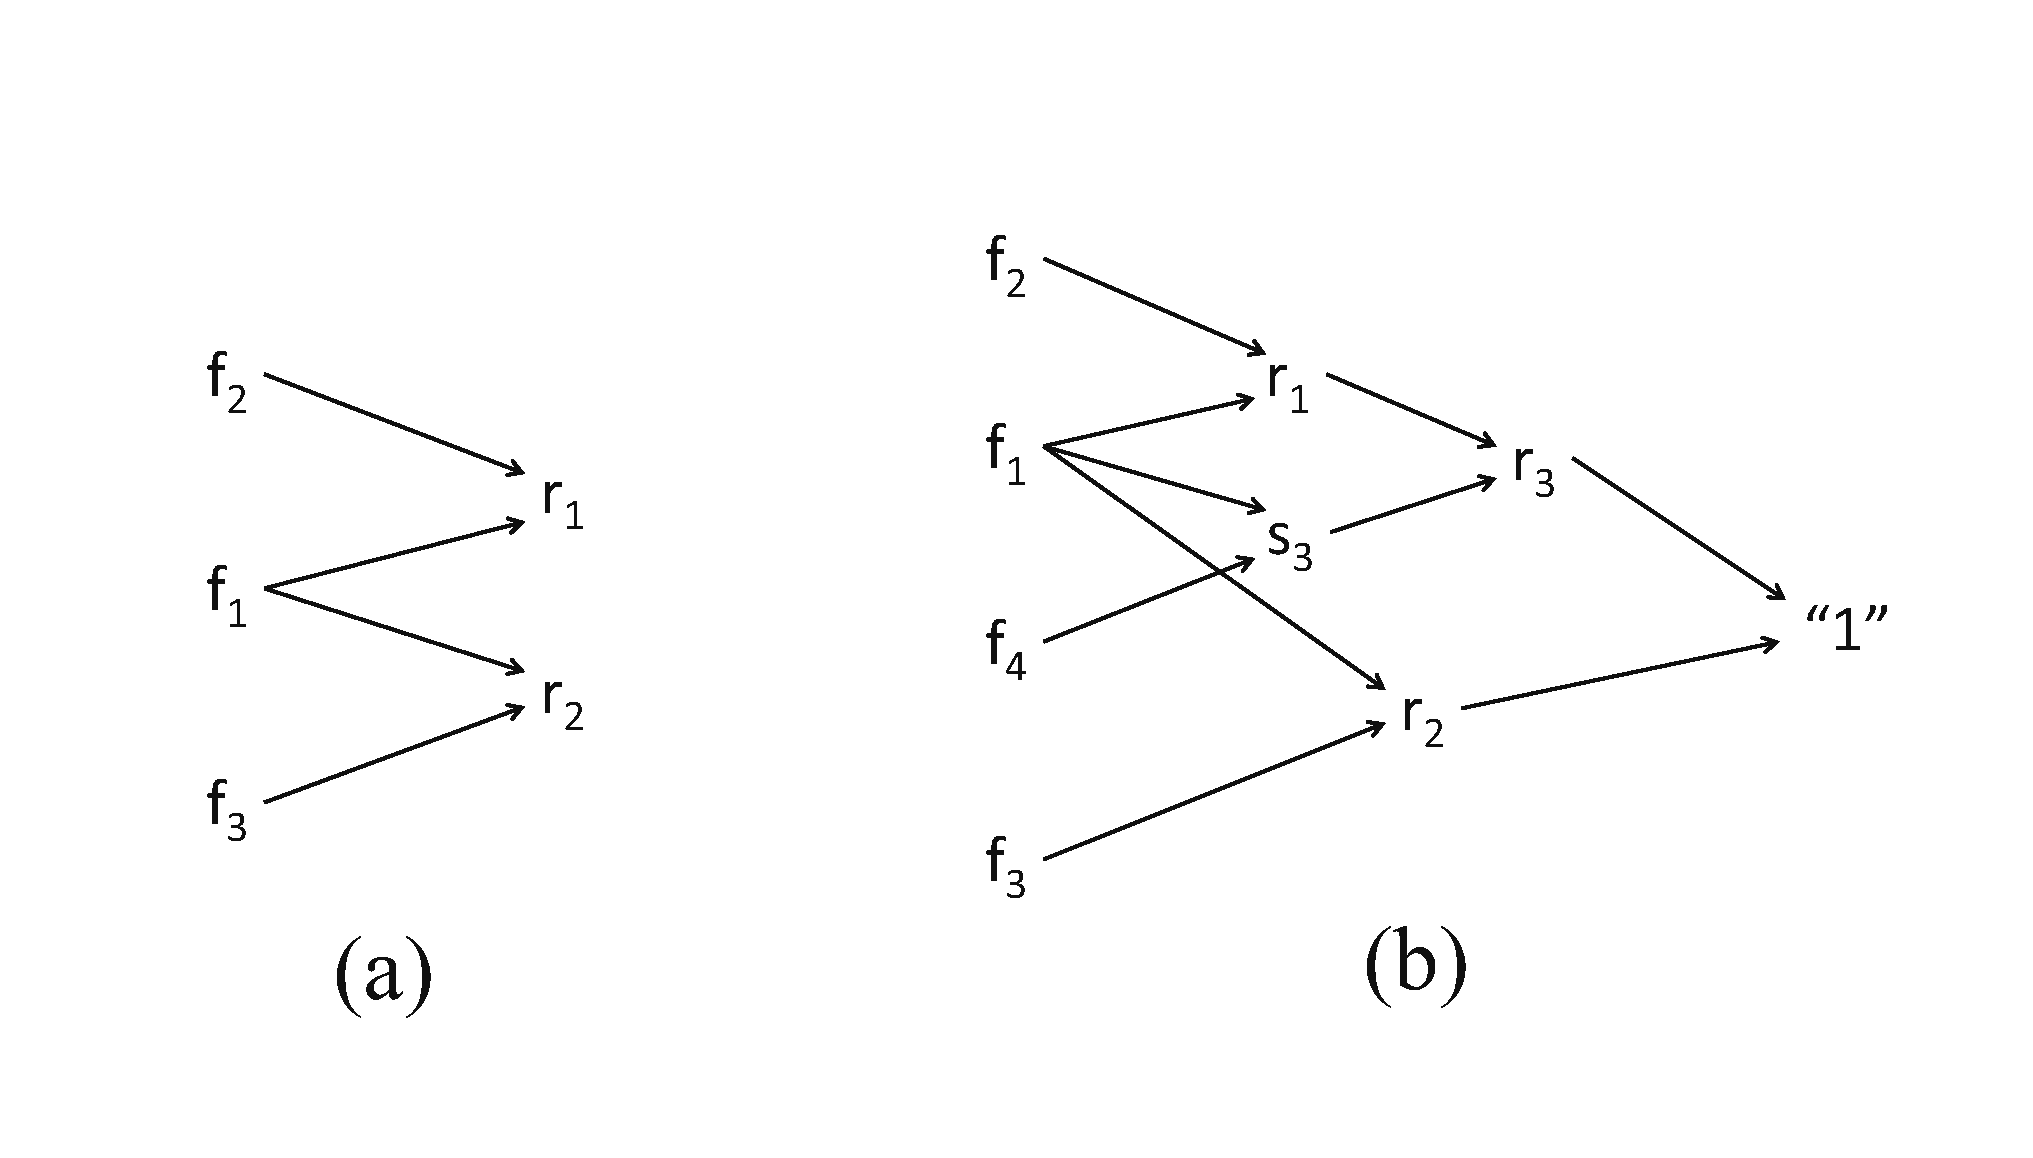
\includegraphics[width=\textwidth]{newfig/UNSAT.eps}}
\caption{DAG representing $Spoly$ computations and multivariate divisions.}
\label{fig:originUNSAT}
\end{figure}

This general idea is depicted in Algorithm \ref{alg:UNSAT}. 
We now show a formal and efficient implementation.

\begin{algorithm}[hbt]
\SetAlgoNoLine
\LinesNumbered
	\KwIn{A set of polynomials $F = \{f_1,f_2,\dots,f_s\}$}
	\KwOut{An UNSAT core $\{f_{m_1},f_{m_2},\dots,f_{m_t}\}$}
\Repeat{$r_l == 1$}
{
	Pick a pair $f_i,f_j\in F$ that has never been computed $Spoly$\;
	\If{$Spoly(f_i,f_j)\xrightarrow{F}_+ r_l \neq 0$}
	{
		$F = F\cup r_l$\;
		Create a DAG $G_l$ with $f_i,f_j$ as roots, $r_l$ as leaf, recording the $Spoly$, all intermediate remainders and $f_k\in F$ that cancel monomial terms in the $Spoly$\;
	}
}
Backward traverse the DAG for remainder ``1", replace $r_l$ with corresponding DAG $G_l$\;
\Return{All roots}
\caption {Extract UNSAT core using a variation of Buchberger's algorithm}\label{alg:UNSAT}
\end{algorithm}

\subsection{The Refutation Tree of the GB Algorithm: Find $F_c$ from $F$}

We investigate whether it is possible to identify a core by analyzing the
$Spoly(f_i,f_j)\xrightarrow{F}_+ g_{ij}$ reductions in Buchberger's
algorithm. Since $F$ is itself an UNSAT core, 
definitely {\it there exists  
a sequence of $Spoly$ reductions in Buchberger's algorithm where
$Spoly(f_i, f_j) \xrightarrow{F}_+ 1$ is achieved.} Moreover, 
polynomial reduction algorithms can be suitably modified to record
which polynomials from $F$ are used in the division leading to
$Spoly(f_i,f_j)\xrightarrow{F}_+1$. This suggests that 
we should be able to identify a core by recording
the {\it data} generated by Buchberger's algorithm --- namely, the
critical pairs($f_i,f_j$) used in the $Spoly$ computations,
and the polynomials from $F$ used to cancel terms in the reduction
$Spoly(f_i,f_j)\xrightarrow{F}_+1$. The following example motivates
our approach to identify  $F_c \subseteq F$ using this data:

\begin{Example}
\label{ex:1}
Consider the following set of polynomials $F = \{f_1,\dots, f_9\}$:

\begin{minipage}{2in}
\begin{align*}
f_1&: abc + ab + ac + bc \\
   & + a + b + c + 1\\
f_2&: b\\
f_3&: ac\\
f_4&: ac + a
\end{align*}
\end{minipage}
%\hspace{0.1in}
\begin{minipage}{3in}
\begin{align*}
f_5&: bc + c\\
f_6&: abd + ad + bd + d\\
f_7&: cd\\
f_8&: abd + ab + ad + bd + a + b + d + 1\\
f_9&: abd + ab +bd + b
\end{align*}
\end{minipage}



Assume $>_{DEGLEX}$ monomial ordering with $a>b>c>d$. 
Let $F = \{f_1,\dots,f_9\}$ and 
$J = \langle F \rangle \subset \mathbb{F}_2[a,b,c,d]$ where
$\mathbb{F}_2 = \{0, 1\}$ is the finite field of 2 elements. Then 
$V(J) = \emptyset$ as $GB(J) = 1$.  The set $F$ consists of 4 {\it minimal}
cores: $F_{c1} = \{ f_1,f_2,f_3,f_4,f_7,f_8\}, F_{c2} = \{
f_2,f_4,f_5,f_6,f_8\}, F_{c3} = \{ f_2,f_3,f_4,f_6,f_8\},$ and $F_{c4}
= \{ f_1,f_2,f_4,f_5\}$. 
\end{Example}

Buchberger's algorithm terminates to a unique reduced GB, irrespective
of the order in which the critical pairs $(f_i,f_j)$ are selected and reduced by operation
$Spoly(f_i,f_j)\xrightarrow{F}_+g_{ij}$. Let us suppose that in the GB
computation corresponding to Example \ref{ex:1}, the first 3 critical
{\it Spoly} pairs analyzed are $(f_1, f_2), (f_3, f_4)$, and
$(f_2,f_5)$. It turns out that the $Spoly$-reductions corresponding to
these 3 pairs lead to the unit ideal. Recording the data
corresponding to this sequence of reductions is depicted by means of a
graph in Figure \ref{fig:refute}. We call this graph a {\it refutation tree}. 

\begin{figure}[bp]
\centering{
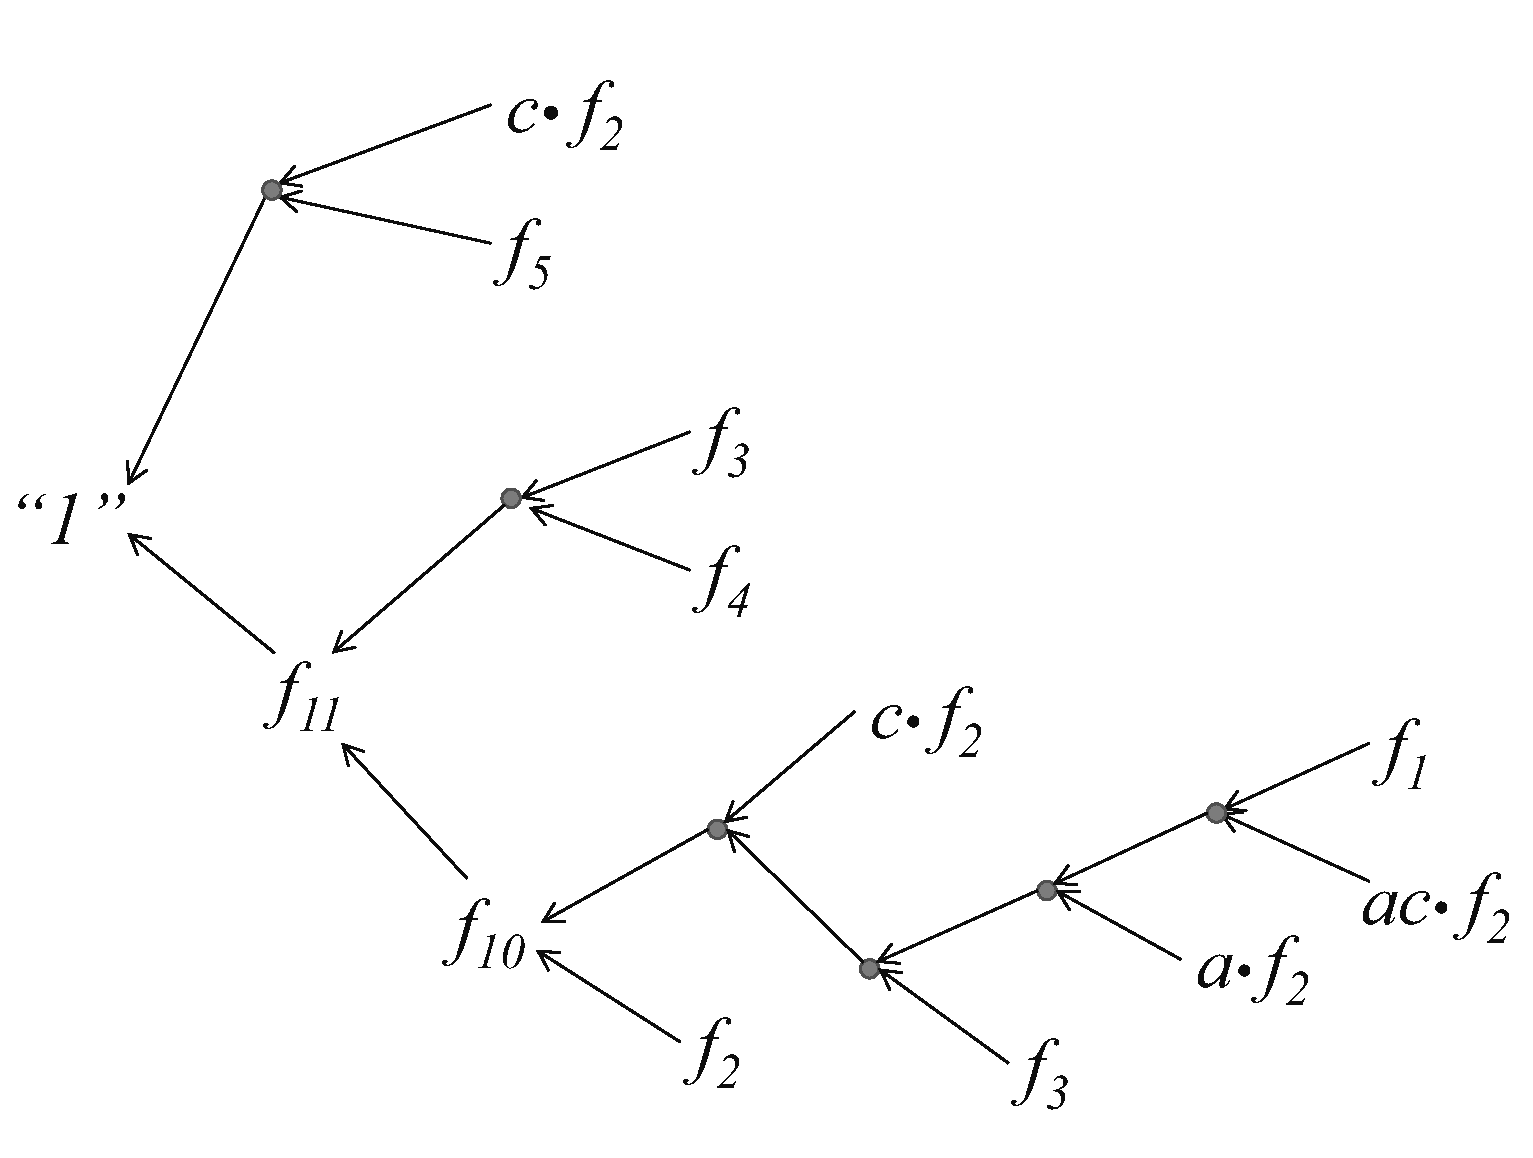
\includegraphics[width=4.5in]{newfig/refutation_tree.eps}}
\caption{Generating refutation trees to record UNSAT cores.}
\label{fig:refute}
\end{figure}

In the figure, the nodes of the graph correspond to the polynomials
utilized in Buchberger's algorithm. The leaf nodes always correspond
to polynomials from the given generating set. An edge $e_{ij}$ from
node $i$ to node $j$ signifies that the polynomial at node $j$ results
from the polynomial at node $i$. For example, consider the computation
$Spoly(f_1,f_2)\xrightarrow{F}_+ f_{10}$, where $f_{10} = a + c +
1$. Since $Spoly(f_1, f_2) = f_1 - ac\cdot f_2$, the leaves
corresponding to $f_1$ and $ac\cdot f_2$ are created. The reduction
$Spoly(f_1,f_2)\xrightarrow{F}_+ f_{10}$ is carried out as the
following sequence of 1-step divisions:
$Spoly(f_1,f_2)\xrightarrow{a\cdot f_2} ~\xrightarrow{f_3}~
\xrightarrow{c\cdot f_2}  ~\xrightarrow{f_2} f_{10}$. This is depicted
as the bottom subtree in the figure, terminating at polynomial
$f_{10}$. Moreover, the multiplication $a\cdot f_2$ implies that
division by $f_2$ resulted in the quotient $a$. The refutation tree of
Figure  \ref{fig:refute} shows further that
$Spoly(f_3,f_4)\xrightarrow{f_{10}} f_{11} = c+1$ and, finally,
$Spoly(f_5,f_2)\xrightarrow{f_{11}} 1$. 
 
To identify an $F_c \subset F$, we start from the refutation node
``1'' and traverse the graph in reverse, all the way up to the
leaves. Then, all the leaves in the transitive fanin of ``1''
constitute an UNSAT core. The polynomials (nodes) that do not lie in
the transitive fanin of ``1'' can be safely discarded from $F_c$. From
Figure \ref{fig:refute}, $F_c = \{f_1,f_2,f_3,f_4,f_5\}$ is identified
as an UNSAT core of $F$. 

\section{Reducing the Size of the UNSAT Core $F_c$}
\label{sec:alg}
The core $F_c$ obtained from the aforementioned procedure may
contain redundant elements which could be discarded. For
example, consider the core $F_c=\{f_1,\dots, f_5\}$ generated in the
previous section. While $F_c$ is a smaller infeasible core of $F$, it
is not minimal. In fact, Example 1 shows that $F_{c4} =\{f_1,f_2,f_4,f_5\}$ is the
minimal core, where $F_{c4} \subset F_{c}$. Clearly, the polynomial
$f_3 \in F_c$ is a redundant element of the core and can be 
discarded. We will now describe techniques to further reduce the size
of the UNSAT core by identifying such redundant elements. 
%how the size of this core could be reduced further.  
For this purpose, we perform a more 
systematic book-keeping of the data generated during the execution of
Buchberger's algorithm and the refutation tree. 

\subsection{Identifying Redundant Polynomials from the Refutation Tree}

We record the S-polynomial reduction
$Spoly(f_i,f_j)\xrightarrow{F}_+{g_{ij}}$, which gives a nonzero
remainder when divided by the system of polynomials $F$ at that
moment. The remainder $g_{ij}$ is a polynomial combination of
$Spoly(f_i,f_j)$ and the current basis $F$; thus, it can be
represented as
\begin{equation}
\label{eqn1}
g_{ij}= S(f_i,f_j)+\displaystyle\sum_{k=1}^m c_kf_k,
\end{equation}
where $0\neq c_k\in\mathbb{F}[x_1,\ldots,x_d]$ and
$\{f_1,\ldots,f_m\}$ is the ``current'' system of polynomials
$F$. For each nonzero $g_{ij}$, we will record the following data: 
\begin{equation}
\label{data1}
((g_{ij})(f_{i},h_{ij})(f_{j},h_{ji})| (c_{k1},f_{k1}),(c_{k2},f_{k2}),\dots,(c_{kl},f_{kl}))
\end{equation}

In Equation \ref{eqn1} and Equation \ref{data1}, $g_{ij}$ denotes the
remainder of the $S$-polynomial $Spoly(f_i,f_j)$ modulo the current system
of polynomials $f_1,\ldots,f_m$, and we denote by  

$$h_{ij}:=\displaystyle\frac{LCM(lm(f_i),lm(f_j))}{lt(f_i)},
h_{ji}:= - \displaystyle\frac{LCM(lm(f_i),lm(f_j))}{lt(f_j)}$$ 
the coefficients of $f_i$, respectively $f_j$, in the $S$-polynomial
$Spoly(f_i,f_j)$. Furthermore, in Equation \ref{data1}, $(c_{k1}, \dots
c_{kl})$ are the respective quotients of division by
polynomials $(f_{k1},\dots,f_{kl})$, generated during the $Spoly$ reduction.  
%polynomial coefficients of  that appear in the
%division process. 

\begin{Example}
Revisiting Example \ref{ex:1}, and Figure \ref{fig:refute}, the data
corresponding to $Spoly(f_1,f_2)$\\$\xrightarrow{F}_+  g_{12} = f_{10}$
reduction is obtained as the following sequence of computations:
$$f_{10}=g_{12}=f_1-acf_2-af_2-f_3-cf_2-f_2.$$ As the coefficient
field is $\mathbb{F}_2$ in this example, $-1 = +1$, so:
$$f_{10}=g_{12}=f_1+acf_2+af_2+f_3+cf_2+f_2$$ is obtained.
The data is recorded according to Equation \ref{data1}:

\begin{center}
$((f_{10}=g_{12}), (f_1,1)(f_2,ac)|(a,f_2),(1,f_3),(c,f_2),(1,f_2))$
\end{center}

\end{Example}

Our approach and the book-keeping terminates when we obtain ``1'' as the
remainder of some S-polynomial modulo the current system of 
generators. As an output of the Buchberger's algorithm, we can obtain
not only the Gr\"obner basis $G = \{g_1,\ldots,g_t\}$, but also a
matrix $M$ of polynomials such that: 

\vspace{-0.1in}
\begin{center}
\begin{align}
   \begin{bmatrix}
           g_{1} \\
           g_{2} \\
           \vdots \\
           g_{t}
         \end{bmatrix}
    &= M \begin{bmatrix}
           f_{1} \\
           f_{2} \\
           \vdots \\
           f_{s}
         \end{bmatrix}
  \end{align}

\end{center}

Each element $g_i$ of $G$ is a polynomial combination of $\{f_1, \dots,
f_s\}$. Moreover, this matrix $M$ is constructed precisely using the
data that is recorded in the form of Equation \ref{data1}. We now give a condition
when the matrix $M$ may identify some redundant elements. 


\begin{Theorem}
\label{thm}
With the notations above, we have that a core for the system of
generators $F = \{f_1,\dots,f_s\}$ of the ideal $J$ is given by the
union of those $f_i$'s from $F$ that appear in the data recorded above
and correspond to the nonzero entries in the matrix $M$.  
\end{Theorem}

\begin{Proof}
In our case, since the variety is empty, and hence the ideal is
unit, we have that $G = \{g_1=1\}$ and $t=1$. Therefore $M=
[a_1, \ldots, a_s]$ is a vector. Then the output of the algorithm
gives: $1 = a_1f_1+\cdots + a_s f_s.$ Clearly, if $a_i=0$ for some $i$ then
$f_i$ does not appear in this equation and should not be included in
the infeasible core of $F$. 

\end{Proof}


\begin{Example}

Corresponding to Example \ref{ex:1} and the refutation tree shown in
Figure \ref{fig:refute}, we discover that the polynomial $f_3$ is used
only twice in the division process. In both occasions, the quotient of
the division is 1. From Figure \ref{fig:refute}, it follows that
\begin{equation}
1 = (f_2 + f_5) + \dots + \mathbf{1\cdot f_3} + \dots + \mathbf{1\cdot
  f_3}+ \dots + (f_1 + f_2)
\end{equation}

Since $1 + 1 = 0$ over $\F_2$, we have that the entry in $M$
corresponding to $f_3$ is 0, and so $f_3$ can be discarded from the
core. 
\end{Example}

\subsection{The GB-Core Algorithm Outline}

The following steps describe an algorithm (GB-Core) that allows us to compute a
refutation tree of the polynomial set and corresponding matrix $M$. 

{\bf Inputs:} Given a system of polynomials $F=\{f_1,\ldots,f_s\}$, a
monomial order $>$ on $\mathbb{F}[x_1,\ldots,x_d]$.  

{\bf S-polynomial reduction:} We start computing the S-polynomials of the system of
generators $\{f_1,\ldots,f_s\}$, then divide each of them by the
current basis $G=\{f_1,\dots,f_s,\dots,f_m\}$, which is the
intermediate result of Buchberger's algorithm.  
In this way, we obtain expressions of the following type:
\begin{equation}
\label{eqn:red}
g_{ij}= \underbrace{h_{ij}f_{i}+h_{ji}f_{j}}_{Spoly(f_i,f_j)}+\displaystyle\sum_{k=1}^m c_kf_k
\end{equation}
If the remainder $g_{ij}$ is nonzero, we denote it by
$f_{m+1}$ and add it to the current set of generators $G$. We
also record the data as in Equation \ref{data1}: 
\begin{displaymath}
((f_{m+1}=g_{ij})(f_{i},h_{ij})(f_{j},h_{ji})| (c_{k1},f_{k1}),(c_{k2},f_{k2}),\dots,(c_{kl},f_{kl}))
\end{displaymath}
This data forms a part of the refutation tree rooted at node $f_{m+1}$.

{\bf Recording the coefficients:} In Equation \ref{eqn:red} we obtain a
vector of polynomial coefficients $c_k$ where $k>s$. These
coefficients are associated with new elements (remainders) in the
Gr\"obner basis that are not a part of the UNSAT core. 
%which cannot benefit the UNSAT core extraction. 
Since each polynomial $f_k$, ($k>s$) is generated by
$\{f_1,\dots,f_s\}$, we can re-express $f_k$ in terms of $\{f_1,\dots,
f_s\}$. Thus, each $f_k, k>s$ can be written as $f_k = d_1f_1 + \dots
+ d_sf_s$. This process adds a new row $(d_1,\dots,d_s)$ to the
coefficient matrix $M$. 


%% Therefore we need to rewrite the vector to
%% one with only $c_k, k=1\dots s$, which can be achieved by substituting $f_k,k>s$ by $f_1,\dots,f_s$:
%% initially we have $f_{s+1}= c_1f_1 + c_2f_2 + \cdots + (h_{ij}+c_i)f_{i}+\cdots+(h_{ji}+c_j)f_{j}+\cdots+c_sf_s$,
%% inductively if we can present $f_{s+1}$ to $f_{s+k-1}$ by $f_1,\dots,f_s$, we can also rewrite
%% $f_{s+k} = d_1f_1+\cdots+d_sf_s$. Then we add a new row $ (d_1,\dots,d_s ) $ to coefficient matrix $M$.

{\bf Termination and refutation tree construction:} We perform
S-polynomial reductions and record these coefficients  generated
during the division until the remainder $f_m = 1$ is encountered. The
corresponding data is stored in a data-structure $D$ corresponding to
Equation \ref{data1}. The matrix $M$ is also constructed. From this
recorded data the refutation tree can be easily derived. 

%the algorithm
%will generate a set of new generators $G$ and coefficient matrix $M$.
%Meanwhile we can construct the refutation tree with the recorded data.
We start with the refutation node ``$f_m=1$'':
\begin{displaymath}
((f_{m}=1)(f_{i},h_{ij})(f_{j},h_{ji})| (c_{k1},f_{k1}),(c_{k2},f_{k2}),\dots,(c_{kl},f_{kl}))
\end{displaymath}
and recursively substitute the expressions for the polynomials $f_k$
($k>s$) until we obtain the tree with all the leaf nodes corresponding
to the original set of polynomials $\{f_1,\dots,f_s\}$. Algorithm
\ref{algo:gbcore} describes this data recording through which the
refutation tree $T$ and the matrix $M$ is derived. 

\begin{algorithm}[H]
 \caption{GB-core algorithm (based on Buchberger's algorithm)}
 \label{algo:gbcore}
 \begin{algorithmic}[1]

 \REQUIRE $F = \{f_1, \dots, f_s\} \in \F[x_1, \dots, x_d], f_i\neq 0$
 \ENSURE Refutation tree $T$ and coefficients matrix $M$
 \STATE{ {Initialize: list $G \gets F$; Dataset $D\gets \emptyset$; $M\gets s\times s$ unit matrix} }
 \FOR {{ each pair $(f_i,f_j)\in G$  }}
 	\STATE  $f_{sp},(f_{i},h_{ij})(f_{j},h_{ji}) \gets Spolyf_i,f_j)$ \COMMENT{$f_{sp}$ is the S-polynomial}
 	\STATE{{ $g_{ij}|(c_{k1},f_{k1}),\dots,(c_{kl},f_{kl}) \gets (f_{sp}\xrightarrow{G}_+  g_{ij})$}}
 	\IF{{ $g_{ij} \neq 0$ }}
 		\STATE {{$G \gets G \cup g_{ij}$}}
 		\STATE {{$D \gets D \cup
                    ((g_{ij})(f_{i},h_{ij})(f_{j},h_{ji})|
                    (c_{k1},f_{k1}),(c_{k2},f_{k2}),\dots,(c_{kl},f_{kl}))$}}
                \STATE{{Update matrix $M$}}
 	\ENDIF
 	\IF {{$g_{ij} = 1$}}
 		\STATE {{Construct $T$ from $D$}}
 		\STATE {{ Return($T,M$) }}
 	\ENDIF
 \ENDFOR
 \end{algorithmic}
 \end{algorithm}


Notice that the core can actually be derived directly from the matrix 
$M$. However, we also construct the refutation tree $T$ as it
facilitates an iterative refinement of the core, which is described
in the next section. 

\section{Iterative Refinement of the UNSAT Core}
\label{sec:iter}

As with most other UNSAT core extractors, our algorithm also cannot
generate a minimal core in one execution. To obtain a smaller core, we
 re-execute our algorithm with the core obtained in the current
iteration. We describe two heuristics that are applied to our
algorithm to increase the likelihood of generating a smaller core in
the next iteration.  

%After eliminating all redundant polynomials, we can call our GB engine
%with the new core. 
An effective heuristic should increase the chances that the refutation
``1'' is composed of fewer polynomials.  In our GB-core algorithm, we
use a strategy to pick critical pairs such that polynomials with
larger indexes get paired {\it later} in the order:
$$(f_1,f_2)\to(f_1,f_3)\to(f_2,f_3)\to(f_1,f_4)\to(f_2,f_4)\to\cdots$$

Moreover, for the reduction process
$Spoly(f_i,f_j)\xrightarrow{F}_+g_{ij}$, we pick divisor polynomials from
$F$ following the increasing order of polynomial indexes. Therefore,
by relabeling the polynomial indexes, we can affect their
chances of being selected in the UNSAT core. We use two criteria to
to affect the polynomial selection in the UNSAT core. One corresponds
to the \emph{refutation distance}, whereas the other corresponds to
the {\it frequency} with which a polynomial appears in the refutation
tree.  

\begin{Definition}[Refutation Distance]
Refutation distance of a polynomial $f_i$ in a refutation tree
corresponds to the number of edges on the shortest path from refutation
node ``1'' to any leaf node that represents polynomial $f_i$. 
\end{Definition}

On a given refutation tree, polynomials with shorter refutation
distances are used as divisors in later stages of polynomial
reductions, which implies that they may generally have lower-degree
leading terms. This is because we impose a degree-lexicographic term
order, and successive divisions (term cancellations) reduce the degree
of the remainders. However, what is more desirable is to use these
polynomials with lower-degree leading terms earlier in the reduction,
as they can cancel more terms. This may prohibit other (higher-degree)
polynomials from being present in the UNSAT core. 


%% So polynomials with lower degree
%% leading terms are more  likely to be used as divisors in later steps
%% of reduction.  
%% In other words, polynomials with shorter refutation
%% distance may have lower-degree leading terms. 
%% If lower degree
%% polynomials are used earlier in the division process, they can cancel
%% more terms, and they will appear in the tree more often --- which may
%% imply that they are a part of the core. 
% %such that the probability that they appear in
%the refutation tree is larger.  

Similarly, we can define the concept of another heuristic:
\begin{Definition}[Frequency of Occurrence]
The frequency of occurrence of a polynomial $f_i$ in a refutation tree
corresponds to the number of times it appears in the refutation tree. 
\end{Definition}

The motivation for using the \emph{frequency of occurrence}
of $f_i$ in the refutation tree is as follows: polynomials that appear
frequently in the refutation tree may imply that they have certain
properties (leading terms) that give them a higher likelihood of being
present in the UNSAT core. 

%make them "favourable" in the unsat core
%selection. For example, their leading terms may contain variables
%that are require them to be included in the minimal core. 

We apply both heuristics: After the first iteration of the GB-core
algorithm, we analyze the refutation tree $T$ and sort the polynomials
in the core by the refutation distance criterion, and use the
frequency criterion as the tie-breaker. The following example
illustrates our heuristic.  


%\vspace{5mm}\\
\begin{Example} 
Consider a set of 6 polynomials over $\F_2$ of an
infeasible instance.
\begin{align*}
f_1: x_1x_3+x_3; & ~~~f_2: x_2 + 1\\
f_3: x_2x_3+x_2; & ~~~f_4: x_2x_3\\
f_5: x_2x_3 + x_2 + x_3 + 1; & ~~~f_6 : x_1x_2x_3 +x_1x_3
\end{align*}

After the first iteration of the GB-core algorithm, the core is
identified as $\{f_1, f_2,f_3,f_4\}$, and we obtain a
refutation tree as shown in Figure \ref{fig:refine}(a).  
\begin{figure}[bp]
\centering{
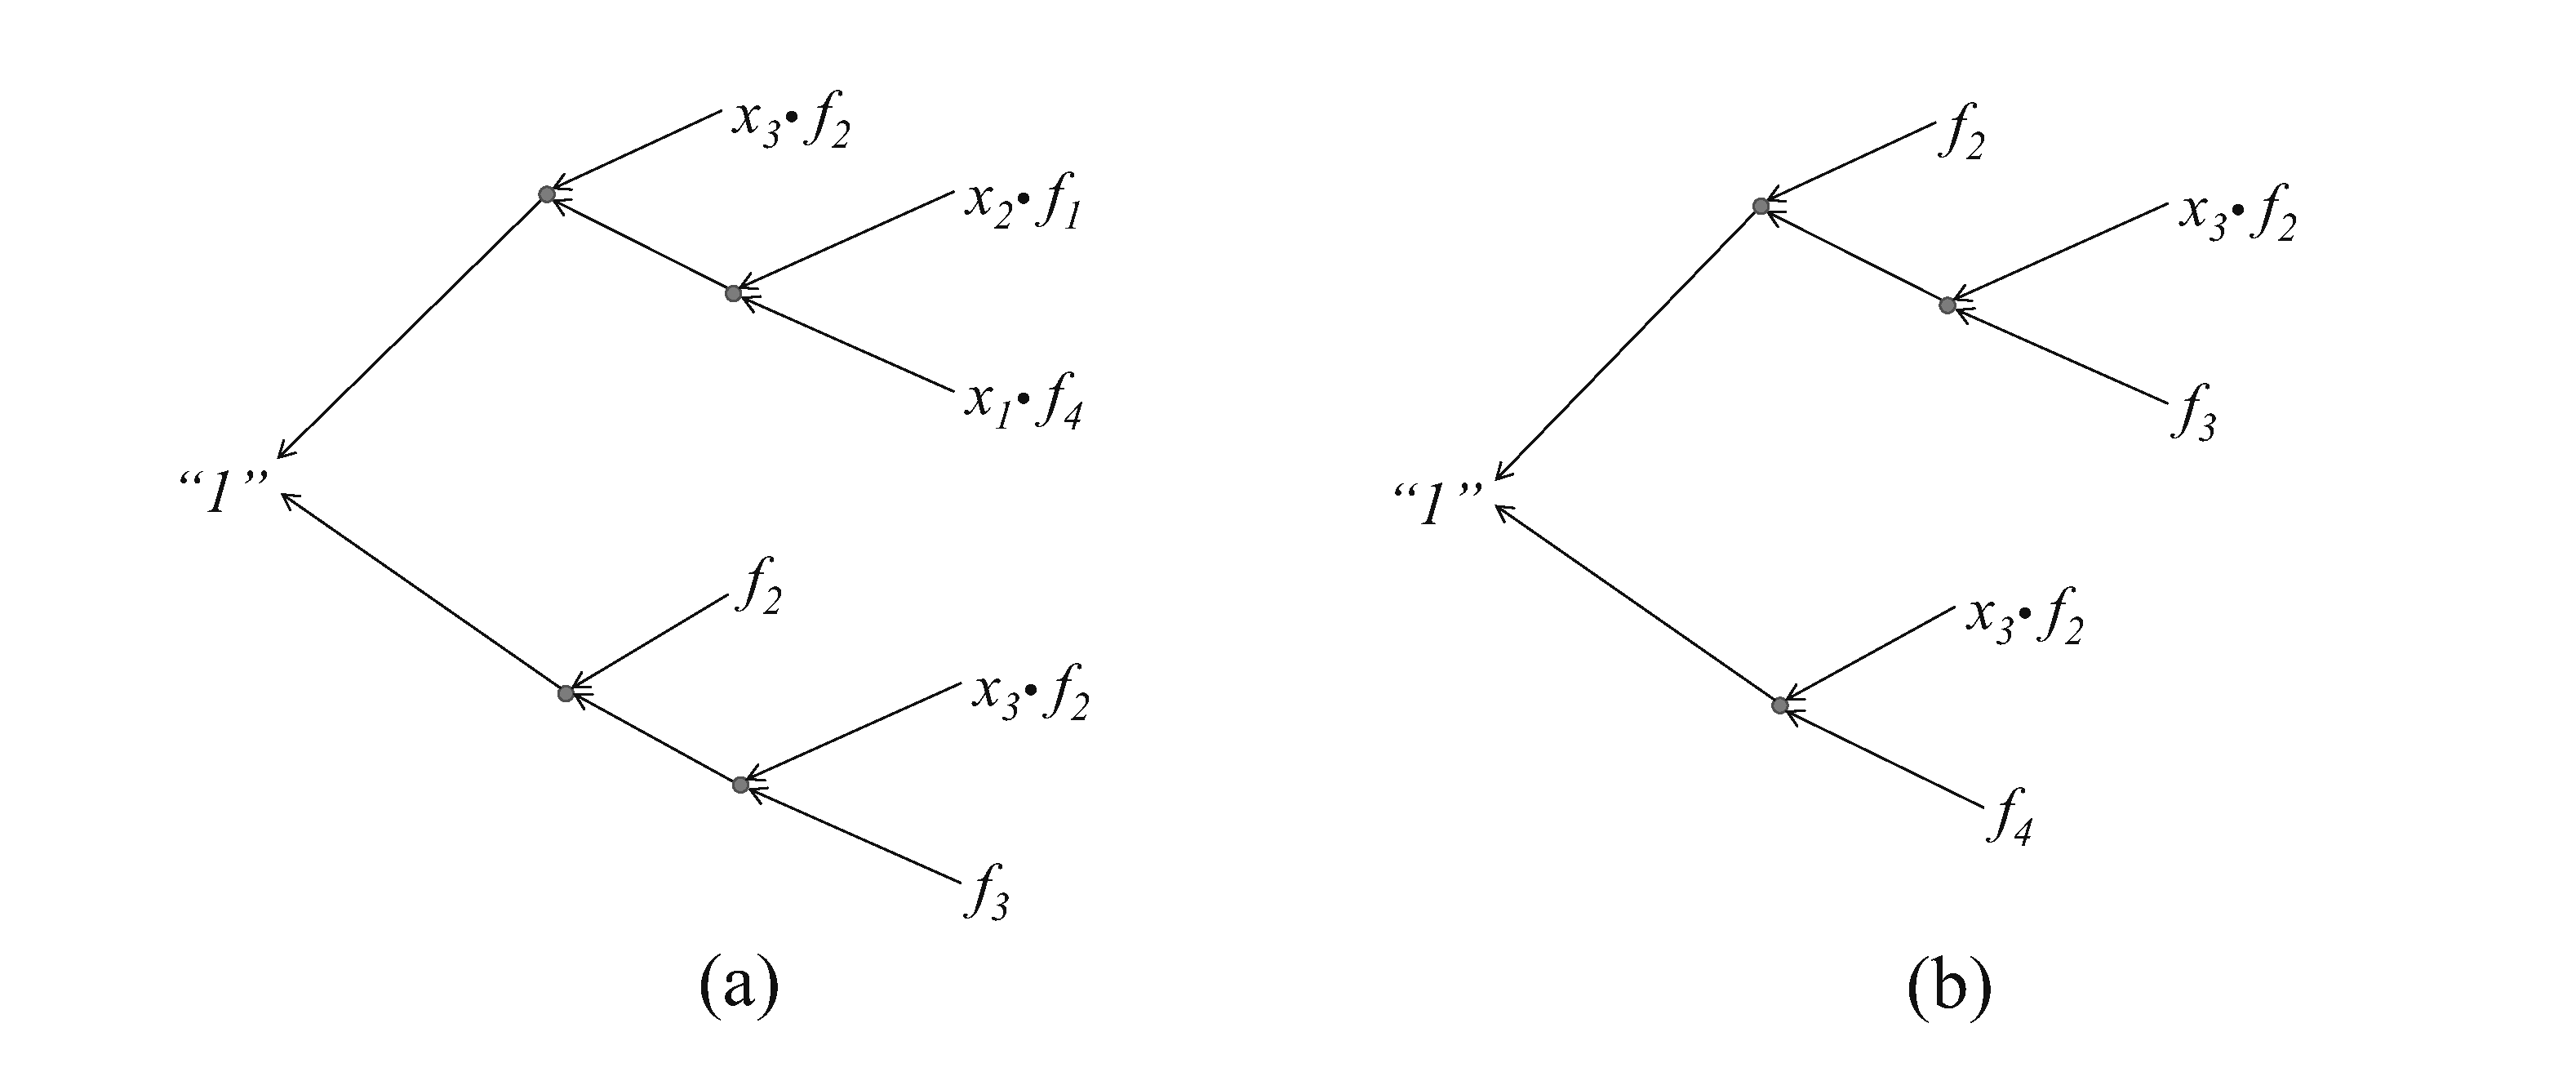
\includegraphics[width=\textwidth]{newfig/core_refine.eps}}
\caption{Refutation trees of core refinement example.}
\label{fig:refine}
\end{figure}

The refutation distance corresponding to polynomial $f_2$ is equal to
2 levels. Note that while three leaf nodes in Figure \ref{fig:refine} (a)
correspond to $f_2$, the shortest distance from ``1'' to any $f_2$
node is 2 levels. The refutation distance and frequency measures of
other polynomials are identical -- equal to 3 and 1, respectively --
so their relative ordering is unchanged. We reorder $f_2$ to be the
polynomial with the  smallest index. We reindex the polynomial set 
$f_1'=f_2, f_2' = f_1, f_3' = f_3, f_4' = f_4$
and apply our GB-core algorithm on the core
$\{f_1',f_2',f_3',f_4'\}$. The result is shown in
Figure \ref{fig:refine}(b) with the core identified as $\{f_1', f_3',
f_4'\} = \{f_2,f_3,f_4\}$. Further iterations do not refine the core
-- i.e., a fix point is reached. 
\end{Example}

\section{Refining the UNSAT Core Using Syzygies}
\label{sec:syz}

%% In some
%% cases our iterative core refining algorithm cannot
%% give us the minimal core when it hits the fixpoint.
%% It indicates the limitation of using re-labelling 
%% strategy, therefore a new method to identify the 
%% redundancy in UNSAT core is needed.

The UNSAT core obtained through our GB-core algorithm is by nature a
refutation polynomial equal to 1:  
$$1 = \sum_{i=1}^s c_i\cdot f_i$$
where $0 \neq c_i \in \F[x_1,\dots,x_d]$ and the polynomials
$F = \{f_1,\dots,f_s\}$ form a core. Suppose that a polynomial 
$f_k \in F$ can be represented using a combination of the rest of the
polynomials of the core, e.g.,
$$f_k = \sum_{j\neq k} c_j'f_j.$$

Then we can substitute $f_k$ in terms of the other polynomials in the
refutation. Thus, $f_k$ can be dropped from the core as it is 
redundant. One of the limitations of the GB-core algorithm and the
relabeling/refinement strategy is that they cannot easily identify
such polynomials $f_k$ in the generating set $F$ that can be composed
of the other polynomials in the basis, i.e.,
$f_k \in \langle F-\{f_k\} \rangle$. We present an approach targeted
to identify such combinations to further refine the core. 
 
 %% Since coefficients $\{c_i\}$ are also polynomials in $\mathbb F[x_1,\dots,x_n]$, we can find 
 %% enormous number of combinations of $\{f_i\}$. Consider finding an algorithmic solution to 
 %% this problem without introducing extra search,
 %% we propose to utilize the \emph{syzygies} generated during
 %% executing the GB-core algorithm.
 
During the execution of Buchberger's algorithm, many critical pairs
$(f_i,f_j)$ do not add any new polynomials in the basis when
$Spoly(f_i,f_j)\xrightarrow{F}_+0$ gives zero remainder. Naturally,
for the purpose of the GB computation, this data is
discarded. However, our objective is to gather more information from
each GB iteration so as to refine the core. Therefore, we further
record the quotient-divisor data from S-polynomial reductions that
result in the remainder 0. Every $Spoly(f_i,f_j)\xrightarrow{F}_+0$
implies that some polynomial combination of $\{f_1,\dots,f_s\}$
vanishes: i.e., $c_1f_1 + c_2f_2 + \dots+c_sf_s=0$, for some
$c_1,\dots,c_s$. These elements ($c_1,\dots,c_s$) form a syzygy on $f_1,\dots,f_s$. 

\begin{Definition}[Syzygy \cite{ideals:book}]
Let $F = \{f_1,\dots,f_s\}$. A syzygy on $f_1,\dots,f_s$ is an
$s$-tuple of polynomials $(c_1,\dots,c_s)\in (\F[x_1,\dots,x_d])^s$
such that $\sum_{i=1}^s c_i\cdot f_i = 0$.
\end{Definition}

For each $Spoly(f_i,f_j)\xrightarrow{F}_+0$ reduction, we record the
information on corresponding syzygies as in Equation \ref{eqn:syz}, also
represented in matrix form in Equation \ref{mat:syzygy}:


\begin{equation} \label{eqn:syz}
%\[
 \begin{cases}
 c_1^1f_1+c_2^1f_2+\cdots+c_s^1f_s = 0\\
 c_1^2f_1+c_2^2f_2+\cdots+c_s^2f_s  = 0\\
 \ \ \ \ \ \  \vdots \\
 c_1^mf_1+c_2^mf_2+\cdots+c_s^mf_s = 0  
 \end{cases}
%\]
\end{equation}

%which can be represented in matrix form as:
\begin{center}
\begin{align}
\label{mat:syzygy}
   \begin{bmatrix}
           c_1^1 & c_2^1 & \cdots & c_s^1 \\
           c_1^2 & c_2^2 & \cdots & c_s^2 \\
           \vdots & \vdots & \ddots & \vdots \\
           c_1^m & c_2^m & \cdots & c_s^m
         \end{bmatrix}
    \begin{bmatrix}
           f_{1} \\
           f_{2} \\
           \vdots \\
           f_{s}
         \end{bmatrix}
         &= 0
  \end{align}

\end{center}


\ \\
 Here $\{f_1,f_2,\dots,f_s\}$ is the given core.
 Take one column of the syzygy matrix (e.g., the set of polynomials in $j$-th column
 $c_j^1, c_j^2, \dots, c_j^m$)  and compute its reduced Gr\"obner
 basis $G_r$. If $G_r = \{1\}$, then it means that there exists some
 polynomial vector  $[r_1,r_2,\dots,r_m]$ such that $1 = r_1c_j^1 +
 r_2c_j^2 + \cdots + r_mc_j^m = \sum_{i=1}^m r_ic_j^i.$ 
 If we multiply each row $i$ in the matrix of Equation \ref{mat:syzygy}
 with $r_i$, and sum up all the rows, we will obtain the
 following equation: 
\vspace{-0.2in}
 \begin{center}
\begin{align}
   \begin{bmatrix}
           \sum_{i=1}^m r_ic_1^i & ~~\cdots & ~~ 1 ~~ & ~~ \cdots ~~ & ~~\sum_{i=1}^m r_ic_s^i
         \end{bmatrix}
    \begin{bmatrix}
           f_{1} \\
           f_{2} \\
           \vdots \\
           f_{s}
         \end{bmatrix}
         &= 0
  \end{align}

\end{center}

This implies that 
 $$\sum_{i=1}^m r_ic_1^if_1 + \cdots + f_j
 +\cdots + \sum_{i=1}^m r_ic_s^if_s = 0,$$
or that $f_j$ is a polynomial combination of
$f_1,\dots,f_s$ (excluding $f_j$). Subsequently, we can deduce that $f_j$ can be
discarded from the core. By repeating this procedure, some redundant
polynomials can be identified and the size of UNSAT core can be reduced
further. 

 \begin{Example}
 Revisiting Example \ref{ex:1}, execute the GB-core algorithm and
 record the syzygies on $f_1,\dots,f_s$ corresponding to the
 S-polynomials that give 0 remainder. The coefficients can be
 represented as entries in the matrix shown below. For example, the first
 row in the matrix corresponds to the syzygies generated by
 $Spoly(f_1,f_3)\xrightarrow{F}_+0$.  

\begin{equation}\label{eqn:sm}
% \[
 \begin{blockarray}{cccccccccccc}
  && f_1 & f_2 & f_3 & f_4 & f_5 & f_6 & f_7 & f_8 & f_9 & f_{10} \\
  \begin{block}{cc(cccccccccc)}
  Spoly(f_1,f_3)\ & & 1 & a+c+1 & b+1 &0&0&0&0&0&0&1\\
  Spoly(f_2,f_3)\ & & 0 & ac & b &0&0&0&0&0&0&0\\
  Spoly(f_1,f_4)\ & & 1 & c+1 & 1 &b&0&0&0&0&0&1\\
  Spoly(f_2,f_4)\ & & 0 & ac+a & 0 &b&0&0&0&0&0&0\\
  Spoly(f_1,f_5)\ & & 1 & a+c+1 & 0 &0&a&0&0&0&0&1\\
  \end{block}
  \end{blockarray}
% \]
\end{equation}

Usually, we need to generate extra columns compared to the syzygy
matrix of Equation \ref{mat:syzygy}. In this example, we need to add an
extra column for the coefficient of $f_{10}$. This is because $f_{10}$
is not among the original generating set; however, some S-polynomial
pairs require this new remainder $f_{10}$ as a divisor during
reduction. In order to remove this extra column, we need to turn the
nonzero entries in this column to 0 through standard matrix
manipulations. 

Recall that we record $f_{10}$ in $M$ as a nonzero remainder when
reducing S-polynomial pair $Spoly(f_1,f_2)\xrightarrow{F}_+f_{10}$. We
extract this information from the coefficient matrix $M$:
 $$(1 ~~ac+a+c+1 ~~1 ~~0 ~~0 ~~0 ~~0 ~~0 ~~0 )$$

 It represents $f_{10}$ is a combination of $f_1$ to $f_9$:
 $$f_{10} = f_1 + (ac+a+c+1)f_2 + f_3$$
 It can be written in the same syzygy matrix form (with column
 $f_{10}$ present) as follows:

\begin{equation}\label{sr}%  \[
 \begin{blockarray}{cccccccccccc}
  && f_1 & f_2 & f_3 & f_4 & f_5 & f_6 & f_7 & f_8 & f_9 & f_{10} \\
  \begin{block}{cc(cccccccccc)}
  Spoly(f_1,f_2)& & 1 & ac+a+c+1 & 1 &0&0&0&0&0&0&1\\
  \end{block}
  \end{blockarray}
 \end{equation}

 By adding this row vector (Equation \ref{sr}) to the rows in
 Equation \ref{eqn:sm} corresponding to the nonzero entries in the
 column for $f_{10}$, we obtain the syzygy matrix only for the
 polynomials in the core:
  \[
 \begin{blockarray}{ccccccccccc}
  && f_1 & f_2 & f_3 & f_4 & f_5 & f_6 & f_7 & f_8 & f_9  \\
  \begin{block}{cc(ccccccccc)}
  Spoly(f_1,f_3)\ & & 0 & ac & b &0&0&0&0&0&0\\
  Spoly(f_2,f_3)\  && 0 & ac & b &0&0&0&0&0&0\\
  Spoly(f_1,f_4)\  && 0 & ac+a & 0 &b&0&0&0&0&0\\
  Spoly(f_2,f_4)\  && 0 & ac+a & 0 &b&0&0&0&0&0\\
  Spoly(f_1,f_5)\  && 0 & ac & 1 &0&a&0&0&0&0\\
  \end{block}
  \end{blockarray}
 \]

 We find out there is a ``1" entry in the $f_3$ column. The last row
 implies that $f_3$ is a combination of $f_2, f_5$ ($f_3 = ac f_2 + a
 f_5$), so $f_3$ can be discarded from the core. 

 \end{Example}

The syzygy heuristic gathers extra information from the GB
computation, it is still not sufficient to derive all polynomial
dependencies. In Buchberger's algorithm,  many S-polynomials reduce to
zero, so the number of rows of the syzygy matrix can be much larger than
the size of the original generating set. Full GB computation on each
column of the syzygy matrix can become prohibitive to apply
iteratively. For this reason, we only apply the syzygy heuristic
on the smaller reduced core given by our iterative refinement algorithm.

\textbf{Our Overall Approach for UNSAT Core Extraction:} i) Given
the set $F = \{f_1,\dots,f_s\}$, we apply the GB-core algorithm,
record the data $D, M$ (Section 4) and the syzygies $S$ on
$f_1,\dots,f_s$. ii) From $M$, we obtain a core $F_c \subseteq
F$. iii) Iteratively refine $F_c$ (Section 5) until $|F_c|$ cannot be
reduced further. iv) Apply the syzygy-heuristic (Section 6) to
identify if some $f_k \in F_c$ is a combination of other polynomials
in $F_c$; all such $f_k$ are discarded from $F_c$. This gives us the
final UNSAT core $F_c$. 

\section{Application to Abstraction Refinement}
In this section we apply our UNSAT core extraction approach to the 
$k$-BMC in Algorithm \ref{alg:refined}. This algorithm utilizes UNSAT core to 
remove irrelevant latches (state variables) to
reduce the state space. Since those state variables contribute nothing to the violation of 
property $p$, the abstracted model is a reasonable overapproximation for checking 
$p$ without loss of accuracy. In the following example, we apply the UNSAT core extraction 
approach to a FSM which is complicated for bounded model checking and show the power of 
abstraction refinement to reduce the state space for refined $k$-BMC.

\begin{Example}
Figure \ref{fig:s27} shows a sequential circuit (``s27'' from the
ISCAS benchmark set) with 3-bit state registers
PS = $\{G7,G6,G5\}$ and NS = $\{G13,G11,G10\}$. 
Its underlying FSM contains 8 states, as shown in Figure \ref{fig:s27_stg}

\begin{figure}[tbp]
\centering{
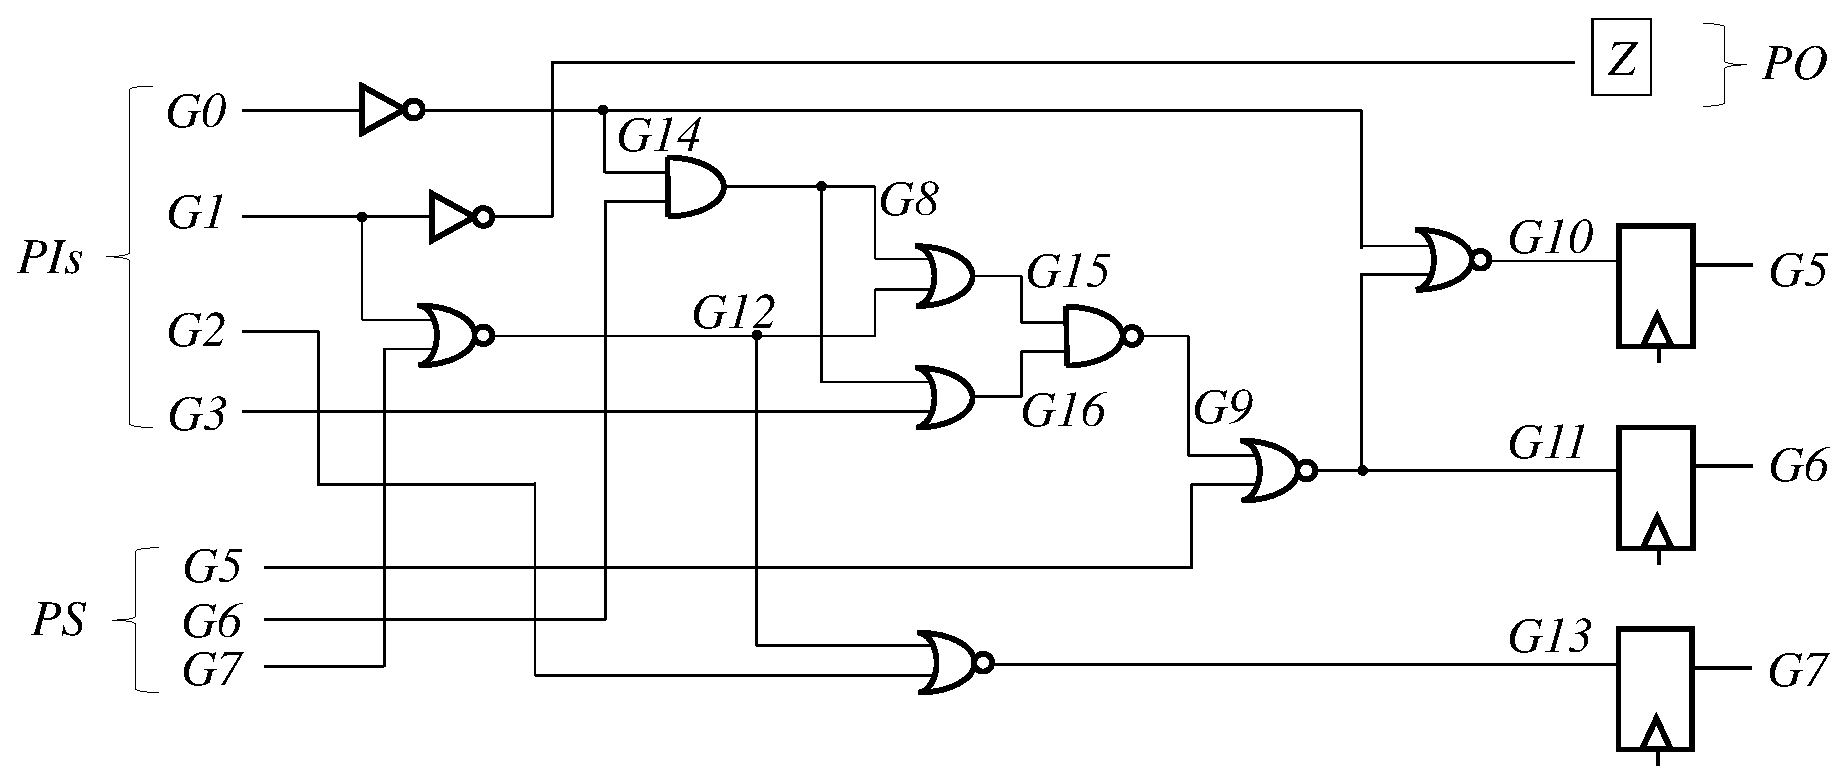
\includegraphics[width=\textwidth]{newfig/s27.eps}}
\caption{Gate-level schematic of the example circuit.}
\label{fig:s27}
\end{figure}

\begin{figure}[tbp]
\centering{
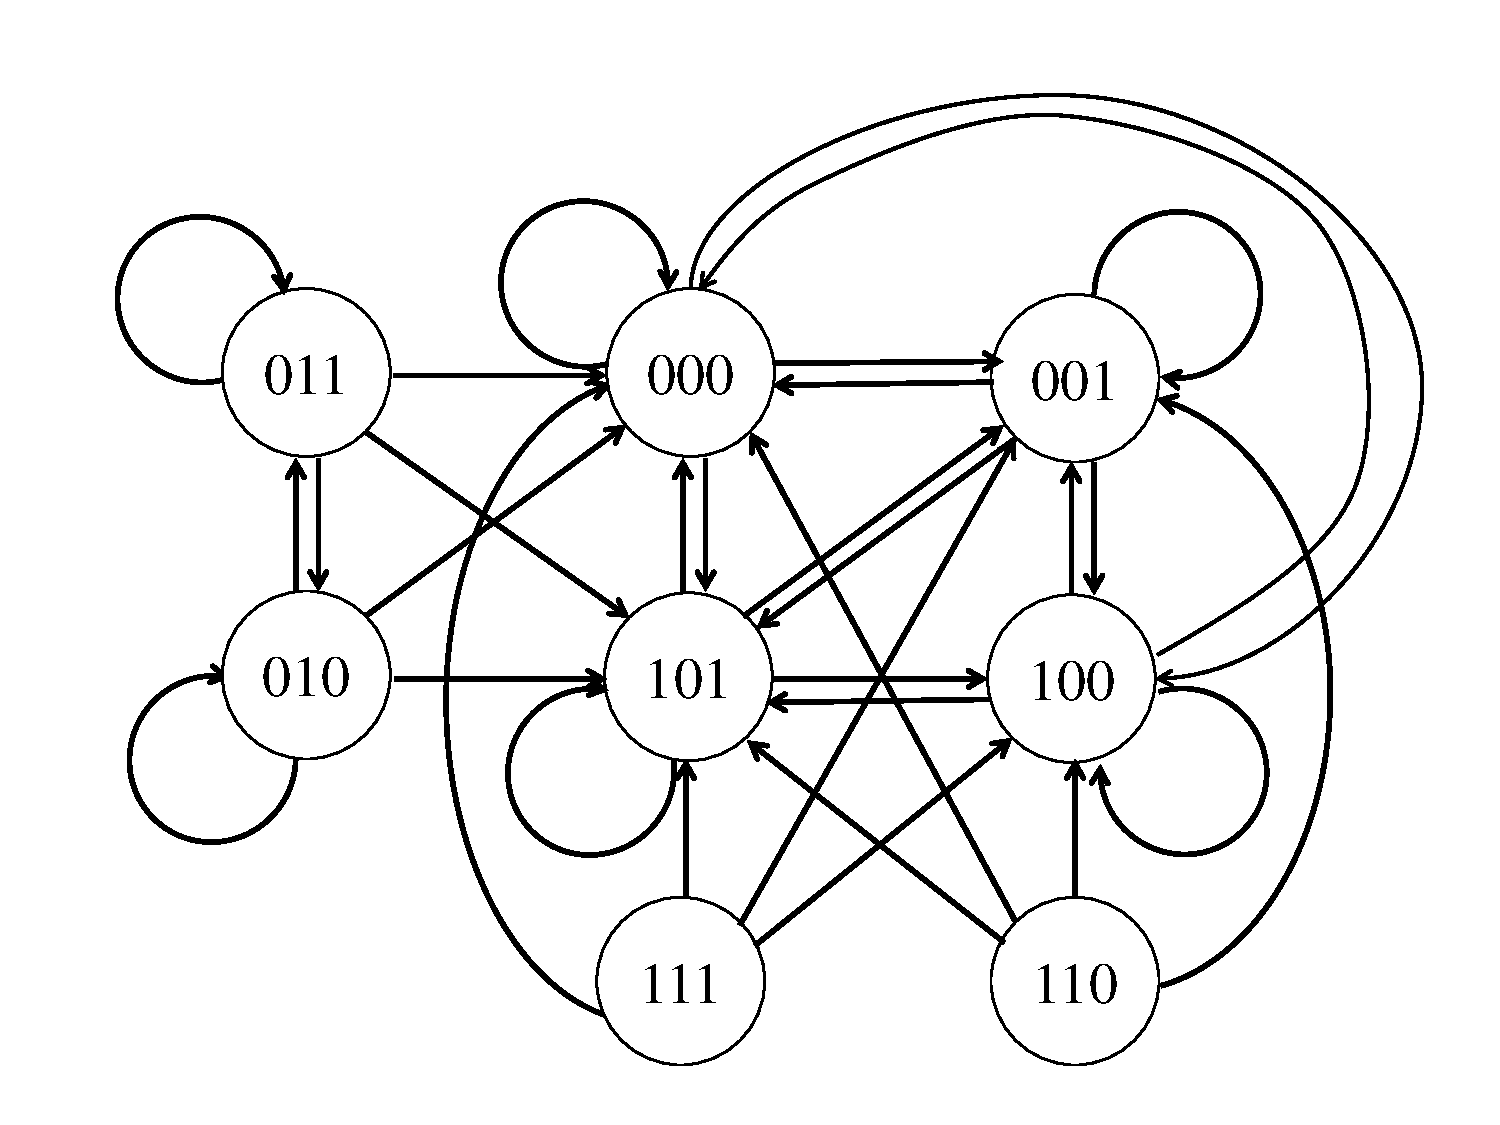
\includegraphics[width=4.5in]{newfig/s27_stg.pdf}}
\caption{State transition graph of example circuit.}
\label{fig:s27_stg}
\end{figure}

On this FSM, define a linear temporal logic (LTL) property 
$$p = {\bf AG}( (\neg G13) {\bf U} (\neg Z) )$$ 
with given initial state $\{000\}$. Model checking on this machine requires
traversal on the STG to search for an accepting trace. If we use $k$-BMC
without abstraction refinement, we need to unroll the machine to
iteration  $k=3$. We show how abstraction will be applied using our
setup.

Because the circuit has 3 latches, we model the problem over the field
${\mathbb{F}}_{2^3}$. First, let the bound $k = 0$. Generate the
polynomial constraints for initial state ideal $I$ and check $SAT(I\land
\neg p)$ using \Grobner bases. The ideal 

\begin{align*}
I = \langle & G14+1+G0, G8+G14\cdot G6, G15+G12+G8+G12\cdot G8,\\ 
	& G16+G3+G8+G3\cdot G8, G9+1+G16\cdot G15, \\ 
	& G10+1+G14+G11+G14\cdot G11, G11+1+G5+G9+G5\cdot G9, \\
	& G12+1+G1+G7+G1\cdot G7, G13+1+G2+G12+G2\cdot G12, \\
	& Z+1+G1, \\
	& \text{(Initial state 000 )} G5, G6, G7 \rangle;
\end{align*}

Property $\neg p$ is also written as a polynomial in the first
time-frame: 
\begin{equation*}
\neg p = Z\cdot G13 + 1
\end{equation*}

As $I\land \neg p$ is UNSAT by the weak
Nullstellensatz, we extract an UNSAT core using our approach:
\begin{align*}
Core(I\land \neg p) =& G12+1+G1+G7+G1\cdot G7, G13+1+G2+G12+G2\cdot G12, \\
& Z+1+G1, G7;
\end{align*}

The result shows that state variables $\{G5,G6, G10,G11\}$ are
irrelevant when considering the violation of $p$. Thus, we can remove
the latches $G10, G11$, and make $G5,G6$ primary inputs. In this way,
the number of state variables is reduced to 1, such that the new
machine only contains 2 states, as the STG in Figure \ref{fig:s27_stg_refined}.

\begin{figure}[tbp]
\centerline{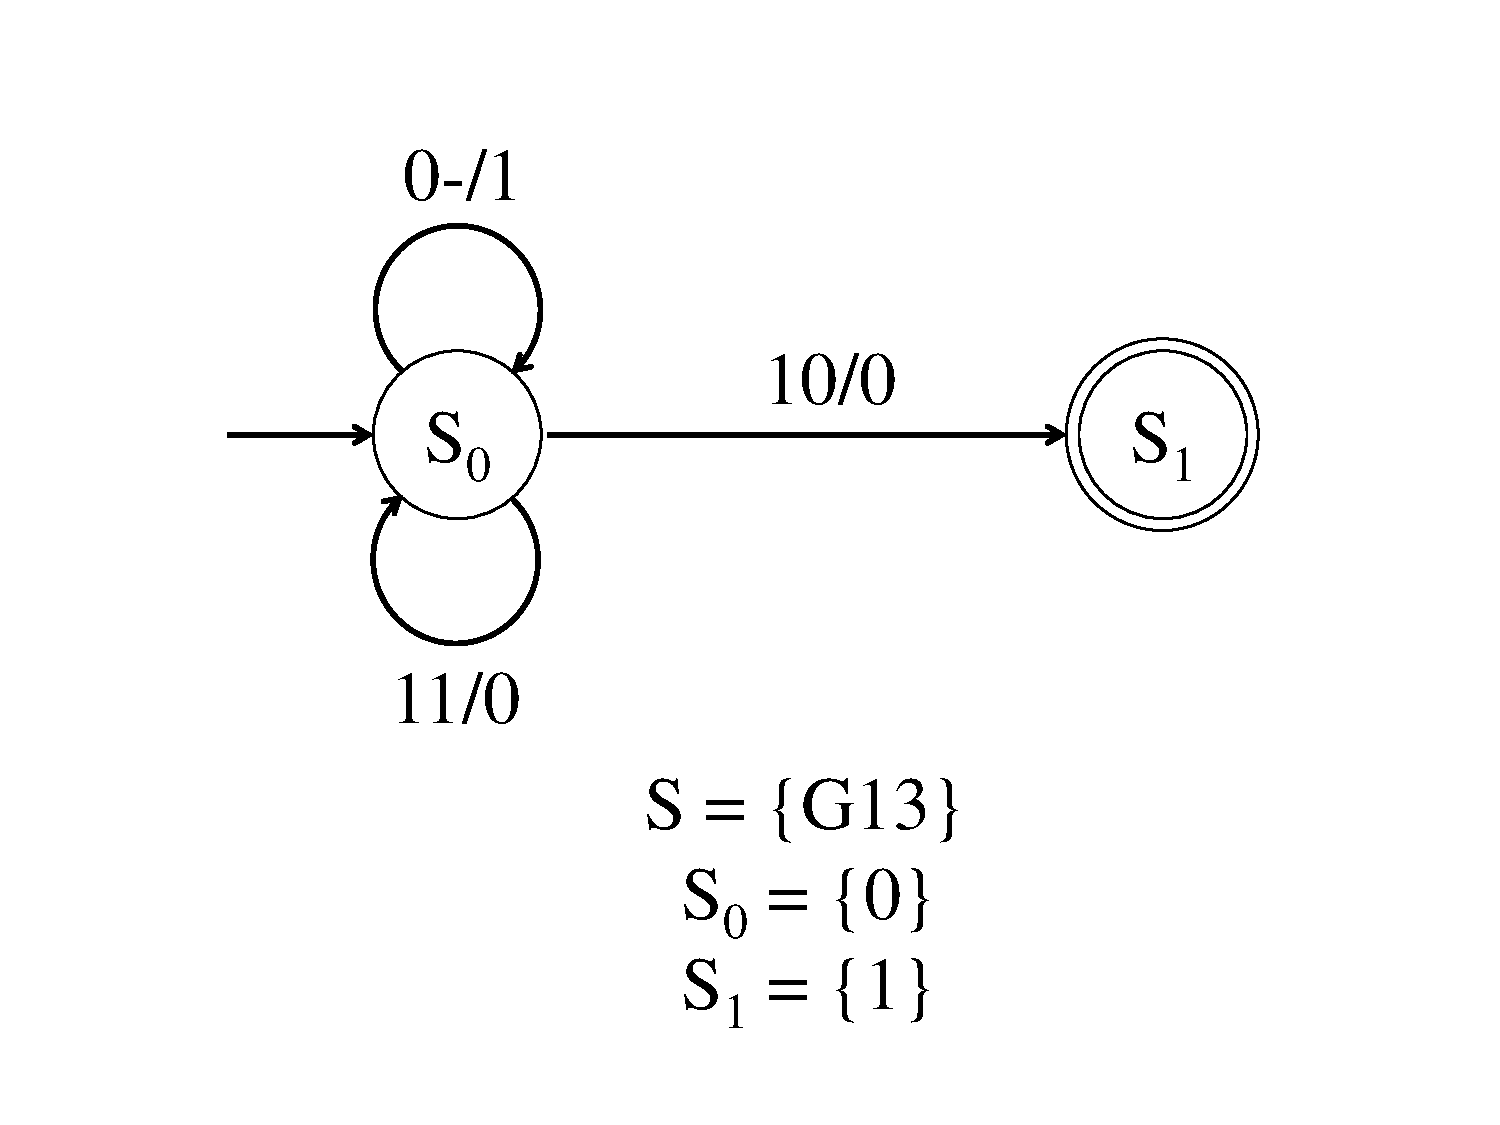
\includegraphics[width=4.5in]{newfig/s27_stg_refined.pdf}}
\caption{State transition graph of abstracted machine.}
\label{fig:s27_stg_refined}
\end{figure}

Since the state space is greatly
reduced, we can execute unbounded model checking on this  abstracted
machine with less cost. As a result, property $p$ is not violated on
the abstracted machine. Therefore, $p$ is also a passing property of
the original machine and  the refined $k$-BMC algorithm terminates!


\end{Example}

\section{Experiment Results}
\label{sec:exp}


We have implemented our core extraction approach (the GB-Core
and the refinement algorithms) using the \textsc{Singular} symbolic
algebra computation system [v. 3-1-6] \cite{DGPS}. With our
tool implementation, we have performed experiments to extract a
minimal UNSAT core from a given set of  
polynomials. Our experiments run on a desktop with
3.5GHz Intel $\text{Core}^\text{TM}$ i7-4770K Quad-core CPU, 16 GB RAM and
64-bit Ubuntu Linux OS. The experiments are shown in Table \ref{tab:result}. 

%Nowadays most SAT benchmarks are huge, which choke our GB engine. 
Gr\"obner basis is not an efficient engine for solving contemporary
industry-size CNF-SAT benchmarks, as the translation from CNF introduces
too many variables and clauses for GB engines to handle. 
On the other hand, although our approach is totally compatible with 
any constraints which can be written as polynomials in GF extensions,
there is no benchmark library clearly identifying a minimal core within 
which to test our tool.

In order to
validate our approach, we make a compromise and create a somewhat customized  benchmark
library by modifying SAT benchmarks and translating from circuit benchmarks: 
1) ``aim-100" is a modified version  of the random 3-SAT
benchmark ``aim-50/100", modified by adding some redundant clauses; 2)
The ``subset" series are generated for random subset sum problems; 3)
``cocktail" is similarly revised from a combination of factorization
and a random 3-SAT benchmark; 4) and ``phole4/5" are generated by
adding redundant clauses to pigeon hole benchmarks; 5) Moreover,
``SMPO" and ``RH" benchmarks correspond to hardware equivalence checking
instances of Agnew's SMPO and RH-SMPO
circuits \cite{agnew1991implementation,RHmulti}, compared against a golden model
{\it spec}. Similarly, the ``MasVMon" benchmarks are the equivalence
checking  circuits corresponding to Mastrovito multipliers compared
against  Montgomery multipliers \cite{lv:tcad2013}. Some of these are
available as CNF formulas, whereas others were available directly as
polynomials over finite fields. The CNF formulas are translated as
polynomial constraints over $\mathbb{F}_2$ (as shown in
\cite{condrat-tacas07}), and the GB-Core algorithm and the refinement
approach are applied.   
%These benchmarks are in moderate size for our GB engine but not too trivial. 

%\vspace{-0.1in}
\begin{table}[tbp]
\centering
\caption{Results of running benchmarks using our tool. 
Asterisk($^*$) denotes that the benchmark was not translated from CNF.
Our tool is composed of 3 parts: part I runs a single GB-core algorithm,
part II applies the iterative refinement heuristic to run the GB-core algorithm
iteratively, part III applies the syzygy heuristic.}
{\small 
\begin{tabular}{|c||c|c|c|c|c|c|c|c|c|c|}
\hline
\multirow{3}{1.8cm}{\centering Benchmark} 
& \multirow{3}{0.7cm}{\centering \# Polys} 
& \multirow{3}{0.7cm}{\centering \# MUS} 
& \multicolumn{3}{c|}{\multirow{2}{1.5cm}{\centering Size of core}}
 & \multirow{3}{1.3cm}{\centering \# GB-core iterations}
 & \multicolumn{3}{c|}{\multirow{2}{1.8cm}{\centering Runtime (sec)}}
 & \multirow{3}{1.6cm}{\centering Runtime of PicoMUS (sec)} \\
  & & &\multicolumn{3}{c|}{}& &\multicolumn{3}{c|}{}& \\
  \cline{4-6} \cline{8-10}
    & & & I & II & III & & I & II & III & \\
\hline
\hline
$5\times 5$ SMPO & 240  & 137  & 169 & 137 & 137  & 8  & 1222 & 1938 & 1698 & $<0.1$\\
$4\times 4$ SMPO$^*$ & 84  & 21  & 21 & 21 & 21 & 1  & 125 & 0.3 & 29  & - \\
$3\times 3$ SMPO$^*$ & 45  & 15  & 15 & 15 & 15  & 1  & 6.6 & 0.2 & 5.7 & - \\
$3 \times 3$ SMPO & 17 & 2 & 2 &2 & 2 & 1 & 0.07 & 0.01 & 0.01  & $<0.1$  \\
$4 \times 4$ MasVMont$^*$ & 148 & 83 & 83 & 83 & 83 & 1 & 23 & 139 & 12 & - \\
$3 \times 3$ MasVMont$^*$ & 84 & 53 & 53 & 53 & 53  & 1 & 4.3 & 4.6 & 0.9  & - \\
$2 \times 2$ MasVMont & 27 & 23 & 24 & 23 & 23 & 2 & 1.3 & 1.0 & 80  & $<0.1$ \\
$5\times 5$ RH$^*$ & 142  & 34  & 48 & 35 & 35  & 4  & 997 & 1.0 & 80 & - \\
$4\times 4$ RH$^*$ & 104  & 35  & 43 & 36 & 36  & 3  & 96 & 5.7 & 0.6 & -\\
$3\times 3$ RH$^*$ & 50  & 20  & 20 & 20 & 20  & 1  &2.9 & 3.5 & 10  & -\\
aim-100 & 79 & 22 & 22 & 22 & 22 & 1  & 43 & 0.7 & 0.2 & $<0.1$\\
cocktail & 135 & 4 & 6 & 4 & 4 & 2 & 51 & 0.01 & 0.01  & $<0.1$ \\
subset-1 & 100 & 6 & 6 & 6 & 6 & 1 & 2.4 & 0.01 & 0.01 & $<0.1$ \\
subset-2 & 141 & 19 & 37 & 23 & 21 & 2 & 12 & 1.6 & 1.1 & $<0.1$  \\
subset-3 & 118 & 16 & 13 & 12 & 11 & 2 & 8.6 & 0.2 & 0.07 & $<0.1$ \\
phole4 & 104 & 10 & 16 & 16 & 10 & 1 & 4.3 & 0.2 & 0.5 &  $<0.1$\\
phole5 & 169 & 19 & 30 & 25 & 19 & 3 & 12 & 3.2 & 2.7 & $<0.1$ \\
\hline
\end{tabular}
}
\label{tab:result}  
\end{table} 

In Table \ref{tab:result}, 
%we list the details of our experimental results. In the table, 
\#Polys denotes the given number of polynomials
from which a core is to be extracted. \#MUS is the {\it minimal} core either
extracted by {\it PicoMUS} (for CNF benchmarks) or exhaustive deletion method (for non-CNF bencmarks).
 \#GB-core iterations corresponds to the
number of calls to the GB-core engine to arrive at the reduced UNSAT
core. The second-last column shows the improvement in the minimal core
size by applying the syzygy heuristic on those cases which cannot be
iteratively refined further. 
We choose {\it PicoMUS} as a comparison to our tool because it is a state-of-art MUS extractor,
and the results it returned for our set of benchmarks are proved to be minimal. 
The data shows that in most of these
cases, our tool can produce a minimal core. For the subset-3
benchmark, we obtain another core with even smaller size than the one from {\it PicoMUS}. The results
demonstrate the power of the Gr\"obner basis technique to identify the
causes of unsatisfiability. 
%From the
%experimental results we can also make the observation that the GB-core
%algorithm, particularly Theorem \ref{thm}, offers quite a lot of scope for identifying redundant
%polynomials that can be eliminated from the core --- without resorting
%to a brute-force membership check of every polynomial $f_i \in F -
%\{f_i\}$. 



\section{Concluding Remarks}\label{sec:conc}
This chapter addresses the problem of identifying an infeasible core of
a set of multivariate polynomials, with coefficients from a field,
that have no common zeros. The problem is posed in the context of
computational algebraic geometry and solved using the Gr\"obner basis
algorithm. We show that by recording the data produced by
Buchberger's algorithm -- the $Spoly(f_i,f_j)$ pairs, as well as the
polynomials of $F$ used in the division process
$Spoly(f_i,f_j)\xrightarrow{F}_+ 1$ -- we can identify certain
conditions under which a polynomial can be discarded from a core. An
algorithm was implemented within the Singular computer algebra tool
and some experiments were conducted to validate the approach. While
the use of GB engines for SAT solving has a rich history, the problem
of UNSAT core identification using GB-engines has not been addressed
by the SAT community. We hope that this technique will kindle some
interest in this topic, which is worthy of attention from the SAT
community -- particularly when there seems to be a renewal of interest
in the use of Gr\"obner bases for formal verification
\cite{lv:tcad2013,gao:qe-gf-gb,kalla:fmcad_tut2015,rolf:date16}.    


\chapter{Conclusions and Future Work}
\label{ch:conclude}
This dissertation presents a new approach to perform reachability
analysis of FSMs at the word-level. It is facilitated by investigating the analog of 
implicit state enumeration algorithm in computer algebra and algebraic
geometry domains. The image function part of the computation is mapped to a variety projection on 
next state variables. This projection is implemented by computing the 
Gr\"obner basis of an elimination ideal with abstraction term orders.
Moreover, the set operations in the state space are mapped to 
the arithmetic of ideals, as algebraic geometry provides a 
way to reason about the variety (solutions) by manipulating the ideals.
A special term order (RATO) is utilized to improve the Gr\"obner bases 
computation, and a tool is developed to implement our 
word-level FSM traversal algorithm. Experiments are performed to 
analyze the reachability for ISCAS'89 and ITC'99 circuit benchmarks.

Next, we describe a method to execute functional verification on sequential Galois field
multipliers over $\Fkk$.  The core algorithm is based on word-level unrolling of 
a Moore machine, which applies concepts from the word-level FSM traversal 
algorithm. As a result, transition relations are represented 
as a polynomial with word-level inputs/outputs.
We implement our algorithm with both the \textsc{Singular} platform and a custom C++ toolset 
and perform experiments on two classes of circuits.
Our approach is able to verify up to 162-bit sequential
circuits, whereas contemporary techniques fail beyond 23-bit
datapaths.  

At last we explore abstraction UNSAT cores in algebraic geometry -- the foundation for refinement techniques
to boost sequential circuit verification.
% UNSAT core extraction, as an indispensable component of many refinement algorithms 
% which rely on UNSAT informations, is thus proposed in polynomial rings.
We use the Weak Nullstellensatz as the essential theory of UNSAT core extraction, 
then develop heuristics to improve the core that exploit the structure of the refutation proof.
An algorithm was implemented within the \textsc{Singular} computer algebra tool
and experiments were conducted to validate the approach.

Our approaches still have limitations: for word-level FSM traversal and 
sequential GF multiplier verification, our methods are more efficient
for XOR-rich circuits, while most industrial designs are AND-OR gate dominant.
For UNSAT core extraction, the abstraction refinement approach such as $k$-BMC 
has only limited application on certain model checking problems. To overcome these limitations,
the following further explorations are worthy of investigation. 
  
\section{Future Work}
In this section, we highlight some research problems that deserve further study.
\subsection{Multivariate Polynomial Ideal based FSM Traversal}
In Chapter \ref{ch:reacha}, we always use a single word-level variable $T$ to denote the
next state. However, in some situations we need to keep recording the relations between $T$ and
inputs, {\it i.e.} the reached states contain multivariate polynomials in $T,S$ and PI $x$. 
While the elimination and set union/intersection are compatible with multiple NS variables,
the set complement requires an extension of Theorem \ref{thm:quotient} on ideals with 
multivariate polynomial generators. We conjecture as follows:

\begin{Conjecture}
Assume we are given ring variables $x_i$, and an ideal $J$ composed by $s$ generators:
$J = \langle f_1,\dots, f_s\rangle$.  Additionally $J_0$ is the vanishing polynomial for variables
$x_i$: $ x_i^{q} - x_i$ where $q$ is the size of signal $x_i$ represents.
We conjecture that
$$V(J') = V(J_0:J) = V(J_0)\setminus V(J) = \overline{V(J)}$$
% And we believe this conjecture is scalable such that it is also valid for even more variables and generators like 
% $J = \langle f_z, v_x,v_y,v_u,v_w\rangle$, $f_z =\mathcal F (z,x,y,u,w)$.
\end{Conjecture}

In univariate case, $\F[x]$ is the principle ideal domain thus Theorem \ref{thm:quotient} can be proved.
However over multivariate case, the proof of this conjecture is not available.

The following example illustrates a different operation from Example \ref{ex:SMPO}.
\begin{Example}
In Figure \ref{fig:fsm}
$\{s_0, s_1\}$ are state/pseudo inputs, $\{t_0,t_1\}$ are state/pseudo outputs, and there is a primary input (1-bit) 
$x$. We propose a new algorithm by modifying Algorithm \ref{alg:univa}:

\IncMargin{1em}
\begin{algorithm}[hbt]
\SetAlgoNoLine
\LinesNumbered
 \KwIn{Transition polynomial $f_t = T + \mathcal F (S,x)$, 
	initial state ideal $from^0 = \langle S+\mathcal G(x), x^{q_1} - x\rangle$}
 \KwOut{Reachable states}
  $reached = from^0(T\setminus S)$\;
  \Repeat{$GB(new^i) == 1$}
  {
  	$i \gets i + 1$\;
	$to^i \gets$GB$(\langle f_t, from^{i-1}\rangle) \setminus \mathcal H(S)$\;
	$\overline{reached} = \langle T^{q_2}-T, x^{q_1} - x \rangle : reached$\;
	$new^i \gets $GB$(to^i + \overline{reached})$\;
  	$reached \gets $GB$( reached \cdot new^i)$\;
	$from^i \gets new^i(S\setminus T)$\;
  }
\Return{$reached$}
\caption {Algebraic Geometry based Traversal Algorithm (multivariate-generator ideals)}\label{alg:multi}
\end{algorithm}
\DecMargin{1em}

The inputs of this algorithm includes transition polynomial (result of word-level abstraction) and initial 
states description ideal, which contains 2 generators corresponds to constraints of PI and combinational input $S$. 
For example, $\langle S+1+\alpha, x^2+x\rangle$ means initial state$=\{11\}$,
$\langle S+x\cdot\alpha, x^2+x\rangle$ means initial states$=\{00,10\}$).

Transition polynomial calculation uses the abstraction and bit-to-level conversion method from 
Chapter \ref{ch:reacha}. After Constructing
an elimination ideal, we impose RATO such that \emph{reverse\ topo\ order\ ckt\ variables }$> T > S > x$, the reduction
remainder has the form $T+\mathcal F(s_0,s_1,x)$. From word definition $S+s_0+s_1\alpha$ we get
$$s_0 = \alpha S^2+ (1+\alpha)S, s_1 = S^2+S$$
Do substitution, the transition polynomial of example ckt is 
$$f_T = T+S^3\cdot x+\alpha S^3+(1+\alpha)S^2\cdot x+S^2+S\cdot x+(1+\alpha)x+1$$

Assume we start from state $\{11\}$. In the first iteration, the reached state is $\{01\}$. Line 4 is to compose an
ideal with 2 generators from $from^0$ and transition polynomial $f_T$, compute its Gr\"obner basis. Note this ideal
has the form
\begin{equation}
I_{tran} = \left\{
             \begin{array}{c}
             T+\mathcal F(S,x) \\
             S + \mathcal G(x) \\
             v_x
             \end{array}  
        \right.
\end {equation}
$v_x$ is a polynomial containing only $q$-bit PI $x$, initially it should be vanishing polynomial $x^{q_1}-x$, 
with the program executing it may be factorized.

Consider Buchberger's algorithm, all generators' leading terms are relatively prime, so it is a GB itself. 
Then we need to reduce this GB, we will find out $S + \mathcal G(x)$ could (possibly) be reduced by $v_x$,
and $T+\mathcal F(S,x)$ will definitely reduced by $S + \mathcal G(x)$. So, at last we will get a polynomial
$T + \mathcal F'(x)$ in reduce GB. We can include this polynomial and $v_x$, exclude the polynomial containing
$S$ (i.e. $\mathcal H(S)$ in algorithm), to compose an ideal representing \emph{next states} $to^i$. 
In iteration 1, result is $to^1 = \langle T+1, x^2+x\rangle$

Line 5 is the ideal quotient of universal set and reached states. In the first iteration, 
$reached$ is the initial state $\langle T+1+\alpha, x^2+x \rangle$. Result of ideal quotient
is $\langle T^3+(1+\alpha)T^2+\alpha T, x^2+x\rangle$ represents $\{00,01,10\}$.

Line 6 is ideals' sum (intersection of their varieties), it is done by combining all generators
from 2 ideals and compute GB. For first iteration result is $GB(\langle T+1,T^3+(1+\alpha)T^2+\alpha T, x^2+x\rangle) = \langle T+1, x^2+x\rangle$ representing $\{01\}$.

Line 7 is ideals' product (union of their varieties), it is done by multiplying all pairs of
generators from both ideal. For first iteration result is $GB(\langle (T+1)(T+1+\alpha),
(T+1)(x^2+x), (T+1+\alpha)(x^2+x), (x^4+x)\rangle) = \langle T^2+\alpha T+(1+\alpha), x^2+x\rangle$ representing $\{01,11\}$.

The traversal will run 3 iterations and terminate at 4th iteration. I list all intermediate 
results below:
\begin{itemize}
\item Iteration 1: $from^0 = \langle S+1+\alpha, x^2+x\rangle, to^1 = \langle T+1, x^2+x\rangle,
 reached = \langle T^2+\alpha T+(1+\alpha), x^2+x\rangle$
\item Iteration 2: $from^1 = \langle S+1, x^2+x\rangle, to^2= \langle T+\alpha, x^2+x\rangle,
reached = \langle T^3+1, x^2+x\rangle$
\item Iteration 3: $from^2 = \langle S+\alpha, x^2+x\rangle, to^3 = \langle T+\alpha x, x^2+x
\rangle, reached = \langle T^3\cdot x+x, T^4+T, x^2+x\rangle$
\item Iteration 4: $from^3 = \langle S, x\rangle, to^4 = \langle T+1, x\rangle, new = \langle1\rangle$
\end{itemize}
The final reachable states are represented by multivariate polynomial ideal $\langle T^3\cdot x+x, T^4+T, x^2+x\rangle$,
which denotes $\{00,01,10,11\}$.
\end{Example}

\subsection{Use of the $F_4$ Algorithm and ZDDs to Accelerate GB Reduction}
In Chapters \ref{ch:reacha} and \ref{ch:normal}, by using RATO we transform the GB-based
computation to that of a multivariate polynomial division. However, this division (reduction)
still incurs exponential complexity in the worst case. In a situation where division is to be performed modulo
a chain of OR gates, the size of remainder polynomial will explode. For example, a chain of OR gates 
can be written as the Boolean function 
\begin{equation}
\label{eqn:chainOR}
f = ((a\lor b) \lor c) \lor d
\end{equation}
which equals to the following polynomial function in $\F_2$:
$$f = abcd+abc+abd+ab+acd+ac+ad+a+bcd+bc+bd+b+cd+c+d$$
Notice, $f$ contains $2^4-1 = 15$ terms, which is exponential in the number of variables.
The size explosion is a major factor affecting the efficiency of polynomial division.

One way to further boost the efficiency is to adopt techniques from sparse linear algebra.
Analysis of experimental results shows that multivariate polynomial division procedure
consumes most of the verification time.
A matrix-based technique named as "$F_4$ style reduction" \cite{f4} can speed up the procedure of
dividing a low-degree polynomial with a term-sparse polynomial ideal. 

Another way is to utilize DDs, {\it e.g.} ZDDs. ZDDs can represent unate covers of Boolean formulas.
We can represent $f$ using a ZDD, where every path in the ZDD from a root to a terminal corresponds
to a monomial term.

\begin{figure}[h]
\centerline{
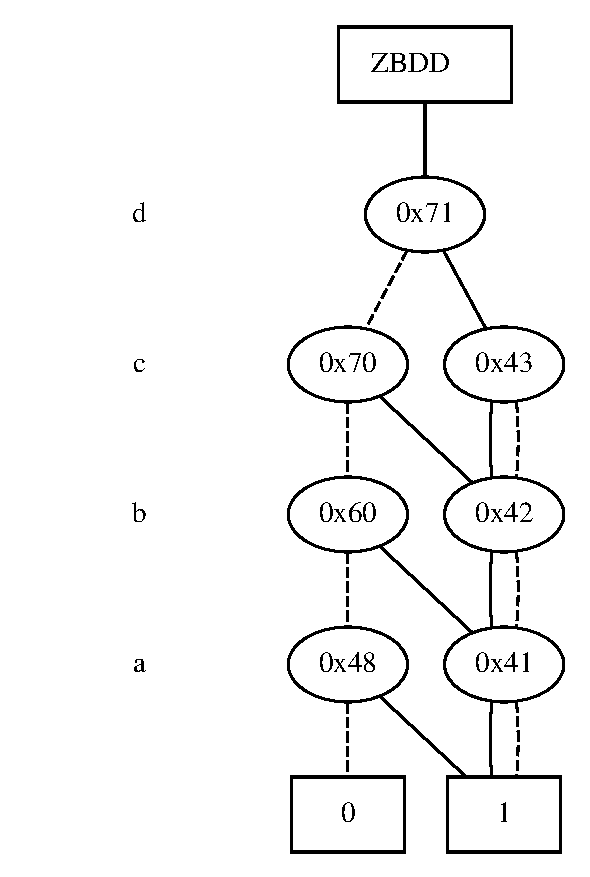
\includegraphics[width=0.35\textwidth]{newfig/ZDD.eps}
}
\caption{A ZDD representing remainder polynomial reducing by a chain of OR gates with order $d>c>b>a$}
\label{fig:ZDD}
\end{figure}

Figure \ref{fig:ZDD} shows a ZDD representing 
Equation \ref{eqn:chainOR} with size $2\times4 -1 = 7$, which is linear in the number of variables.
The reduction process using ZDDs can be executed as in \cite{polybori:2009}. The graphical illustration 
of the remainder in ZDDs is also shown in Figure \ref{fig:ZDD}. 

\subsection{Craig Interpolants in Algebraic Geometry}
The concept of Craig Interpolants (CI) and their existence comes from
symbolic logic \cite{craig-interpolate}; later, algorithms were
presented to find the CI for Boolean formulae
\cite{pudlak:ci} \cite{mcmillan2003interpolation}. Assume that Boolean
formulae are represented in Clause Normal Form (CNF) as 
$f = C_1 \wedge C_2 \wedge \dots \wedge C_m$ where: 1) Each clause
$C_i$ is a disjunction (Boolean OR, denoted $\vee$) of literals; 2)
Each literal is a Boolean variable $x_i$ or its complement
$\overline{x_i}$. 
The Boolean satisfiability (SAT) problem requires that we find an
assignment to the variables such that the formula $f$ is satisfied
(SAT), or otherwise prove that no such assignment exists (UNSAT). 
A CI is related to an UNSAT formula. 

\begin{Definition}
(From \cite{mcmillan2003interpolation}) Let $A$ and $B$ be Boolean
  formulas given as sets of clauses such that $A \wedge B$ is
  unsatisfiable (UNSAT). Then there exists a formula $P$ such that: 
1) $A$ implies $P$ (or $A \subseteq P$); ~2) $P \wedge B$ is UNSAT; ~3)
$P$ refers to only the common variables of $A$ and $B$. The formula
$P$ represents an {\bf interpolant} of $A$ and $B$. 

Given  the pair $(A, B)$ and their refutation proof, a procedure
called interpolation system constructs an interpolant in linear time
and space in the size of the proof \cite{mcmillan2003interpolation}
\cite{pudlak:ci}. 
\end{Definition}

\begin{Example}\label{ex1}
Let $f = (\overline{d})(\overline{c})(\overline{a}\vee d)(a
\vee b \vee c)(\overline{b})$ be a CNF formula. Let $f = A \wedge B =
\emptyset$, where $A = (\overline{d})(\overline{c})(\overline{a}\vee
d)$ and  $B = (a \vee b \vee c)(\overline{b})$. Then $P = \overline{a}
\wedge \overline{c}$ is an interpolant of $(A, B)$. 
\end{Example}

CIs are used to derive abstractions to produce over-approximate image
operators in model checking \cite{mcmillan2003interpolation}. Since $A
\implies P$, $P$ contains $A$ and is an {\it abstraction} of $A$. It
also has fewer variables, so checking  invariants on $P \wedge B$ is
easier. The interpolant is derived through a resolution proof of the
SAT problem. There can be many interpolants $P_i$ for a pair $(A,B)$; 
however, it is not feasible to explore a few or all of these
interpolants by means of the resolution proof. 


We introduce the algebraic geometry analog of CI.
We conjecture that the
  concept of CI should be related to elimination ideals, so future lines
  of investigation should focus on \Grobner basis computations with
  elimination term orders for their computation.



\begin{Definition}\label{ci}
Let $F = \{f_1, \dots, f_s\}$ be a set of polynomials in the ring 
$R = \Fq[x_1,\dots,x_n]$. Let $F = F_A \cup F_B$ and ideals $J =
\langle F \rangle, J_A = \langle F_A \rangle, J_B = \langle F_B
\rangle$ be corresponding ideals in $R$ such that $J = J_A + J_B$. Let
it be known (say, due to application of Weak Nullstellensatz and
Gr\"obner basis) that the varieties $V_{\Fq}(J) = V_{\Fq}(J_A) \cap
V_{\Fq}(J_B) =V_{\Fq}(J_A+J_B)=\emptyset$. Also, let the set of
variables $X = \{x_1,\dots,x_n\} = X_A \cup X_c \cup X_B$ where $X_A,
X_B$ are the set of variables present exclusively in the sets of
polynomials $F_A, F_B$ respectively. Only $X_c$ is the set of
variables that are common to both sets of polynomials $F_A,
F_B$. Then, there exists a set of polynomials  $F_P$ and ideal $J_P =
\langle F_P \rangle$ such that 
\bi
\item $V_{\Fq}(J_A) \subseteq V_{\Fq}(J_P)$
\item $V_{\Fq}(J_P) \cap V_{\Fq}(J_B) = \emptyset$
\item Polynomials of $F_P$ contain the common variables ($X_C$) of
  $F_A, F_B$. 
\ei

We call the ideal $J_P = \langle F_P\rangle$ the {\bf algebraic
  interpolant} of  $J_A+J_B$. 
\end{Definition}

Existence of algebraic interpolant comes from \cite{craig-interpolate}.
The question for exploring is that how do we compute it in algebraic geometry?

\begin{Example} \label{ex2}
Based on Example \ref{ex1}, we translated the system over
$\mathbb{F}_2[a, b, c, d]$. Let $F_A = \{f_1, f_2, f_3\}$ and $F_B =
\{f_4, f_5\}$ where: $f_1: d; ~~~f_2: c; ~~~f_3: a + da; f_4:  abc +
ab + ac + bc + a + b + c + 1; ~~~f_5: b.$ The Boolean interpolant
$\overline{a}\wedge\overline{c}$ from Example \ref{ex1} translates to
${\mathbb{F}}_2$ as the polynomial $f_p = ac + a + c$, with its
variety $V(f_p) = \{a=0, c=0\}$.   
\end{Example}

% {\bf Research problem 2:}
% {\it How can this algebraic interpolant $f_p$ (or in the general case,
%   the set of polynomials $F_P$) be computed? As the interpolant $F_P$ 
% contains only variables $X_C$ that are common to the polynomial sets
% $F_A, F_B$, does this imply that the interpolants can be computed by
% means of \Grobner bases with an elimination term order $X_A>X_B>X_C$
% with $X_A, X_B$ eliminated from the problem? }

Algebraic interpolation is strongly related
to the GB computation with the elimination order $X_A>X_B>X_C$, and
this relationship needs to be formally derived. 

\begin{Conjecture} \label{con:ci}
Computations of algebraic interpolants: Let $J_0$ denote the ideal of
all vanishing polynomials in $\Fkk[x_1,\dots,x_n]$.
\bi
\item  Compute a Gr\"obner basis $G_1 = GB(J_A + J_0)$ 
with the elimination order $X_A > X_B > X_C$, and select
$F_{P1}=G_1\cap\Fkk[X_C]$. We conjecture that the \Grobner
basis $F_{P1}$ of the elimination ideal corresponds to an algebraic
interpolant. 

\item Analogously, compute a Gr\"obner basis $G_2 = GB(J_B + J_0)$ 
with the elimination order $X_B > X_A > X_C$, and select
$F_{P2}=G_2\cap\Fkk[X_C]$. Find an ideal $F'_{P2}$ such that
the variety $V(F'_{P2})$ is the complement of the variety
$V(F_{P2})$. Then the set $F'_{P2}$ gives another interpolant.
\ei
\end{Conjecture}


\begin{Example}\label{ex3}
Consider the polynomials $\{f_1, \dots,f_5\}$ from Example
\ref{ex2}. Computing $F_{P1}$ as described in Conjecture \ref{con:ci} 
produces $F_{P1} = \{a, c\}$, correctly giving us the desired variety
$V(a = 0, c = 0)$. Similarly, when we compute $F_{P2}$, we find that
the interpolant is $ac + a + c + 1$. Notice that the variety 
$V(ac+a+c+1)=\{(0,1), (1,0), (1,1)\}$, which is exactly the complement
of $V(F_{P1})$.  
\end{Example}

The aforementioned experiments in Example \ref{ex3} do not invalidate
our conjectures. Moreover, the above experiment shows that there can be
multiple ways of computing the interpolants. What can these \Grobner
basis computations tell us about the number of valid algebraic
interpolants for any given problem? Can they be classified as {\it weak
  or strong interpolants} based on the sparsity of the polynomials
(power of abstraction)? 

As there can be many interpolants for an ideal-pair $(J_A, J_B)$, 
the following questions should also be investigated in the future:
\bi
\item Find the minimal interpolant: {\it i.e.} find the interpolant $F_P$
  such that $V(J_P)$ is the smallest variety larger than $V(J_A)$ such
  that $V(J_P) \cap V(J_B) = \emptyset$.
\item Analogously, find the maximal interpolant. 
\item Over finite fields, the variety of an elimination ideal is
  exactly equal to the projection of the variety on the remaining
  variables. Consider Figure \ref{fig:projection}, where variety of the
  ideals $J_A, J_B$ are respectively projected on the common variables
  $X_C = \{a, c\}$. Then, does computing $F_{P1}$ (resp. $F_{P2}$) 
  deliver the minimal (resp. maximal) interpolant?
\ei

\begin{figure}[h]
\centering{
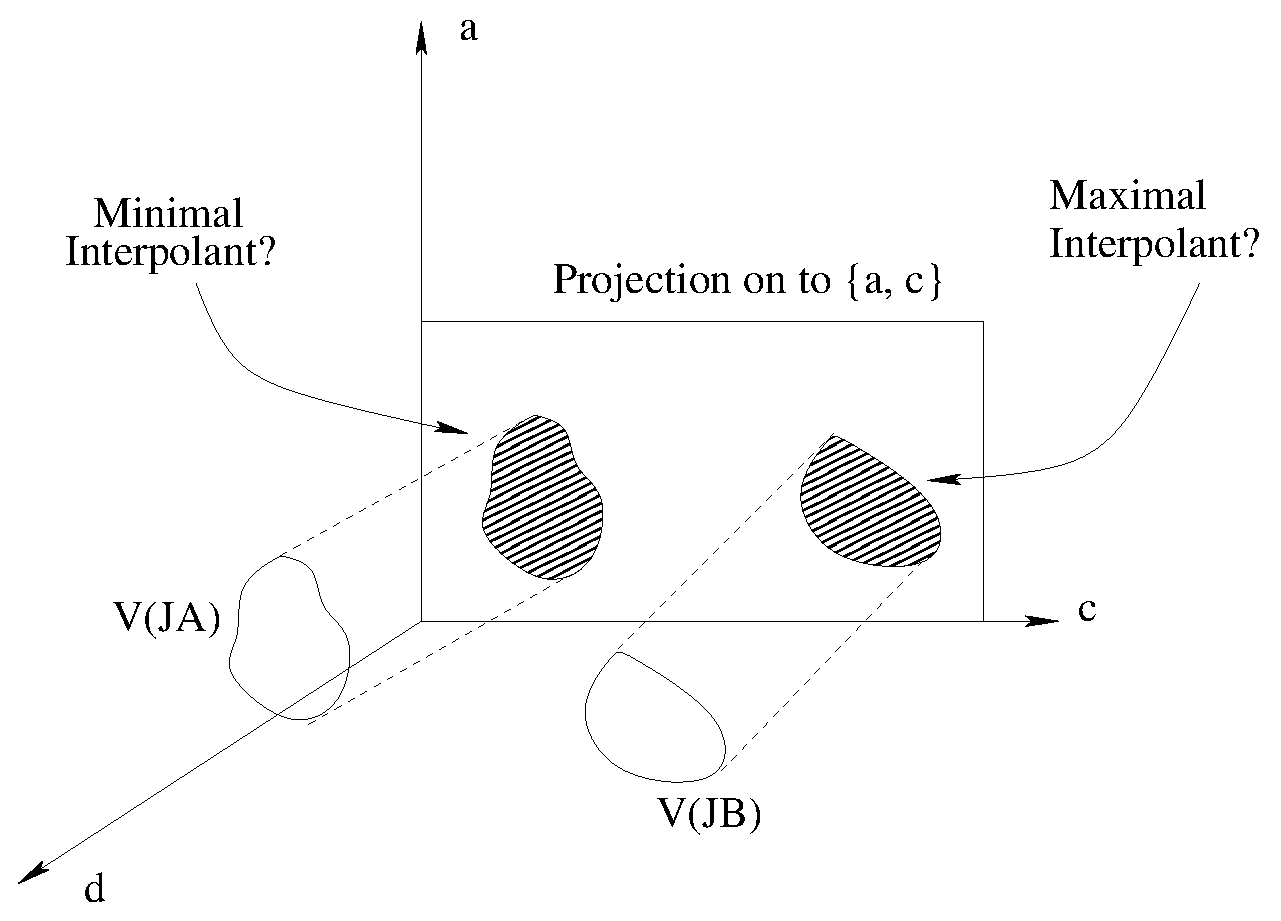
\includegraphics[width=4.5in]{newfig/project.eps}
\caption{Algebraic interpolant: Projection of varieties on common variables }
\label{fig:projection}}
\end{figure}

% 
% Once these problems are understood and algorithms for the computation
% of algebraic interpolants derived, then we will integrate them 
% with word-level reachability analysis for abstraction-based model
% checking. 

\subsection{Technology Mapping for Word-level Functional Blocks}
Technology mapping is an important problem in digital circuit synthesis.
Designers are given a library of well-designed functional/macro blocks (including IP cores) and a raw netlist, 
technology mapping's objective is to map as many as blocks to the raw netlist and 
keep the functional equivalence. Contemporary techniques rely on bit-wise 
analysis on the signals to deduce the boundary of mapped blocks.
It is possible to use the equivalence checking techniques proposed in this dissertation 
as a alternative way to perform technology mapping, especially on word-level when 
given blocks represent word-level functions.

\begin{Problem}
The objective of our approach is to map the macro blocks without boundary information.
Mapping is an essential technique used in synthesis and verification. In synthesis, we can map the 
macro functions with smaller and faster implementations to optimize the timing and area; in simulation,
we can map a complicated function to a simple execution to accelerate simulation speed.

Given a gate-level design $D$ and several word-level macro blocks $\{B_i\}$, we need to map macro
blocks $B_i$ into design $D$, and write out the mapped design $D'$ which is equivalent to original
design $D$. The objective is to generate a mapped design $D$ with as many of $B_i$ such that the area
and timing is optimal. The procedure is also illustrated in Figure \ref{fig:macro}.

\begin{figure}[h]
	\begin{center}
	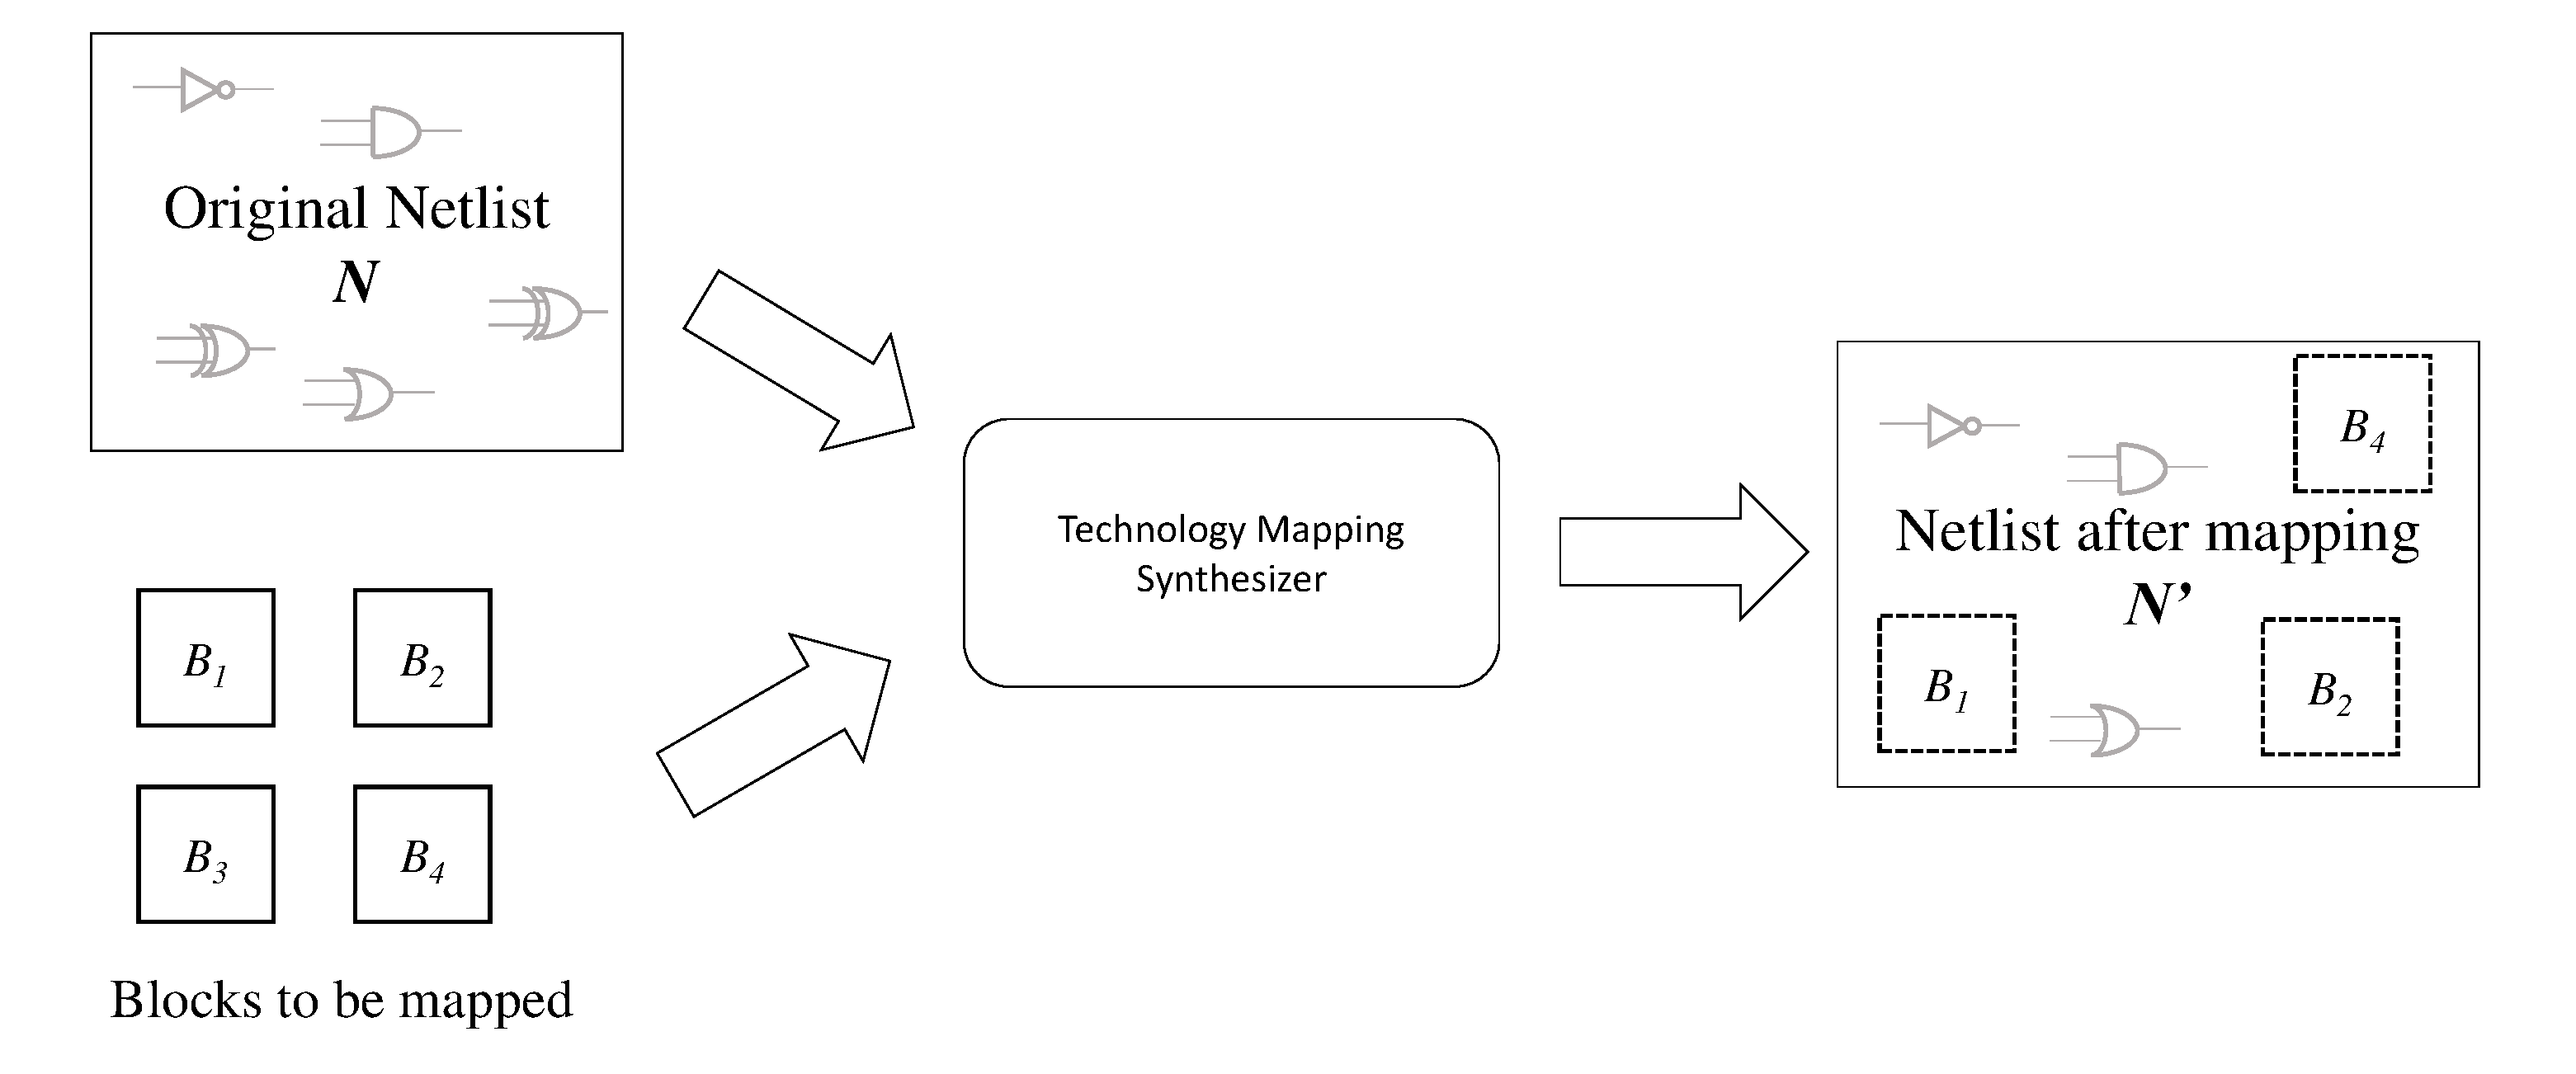
\includegraphics[width=\textwidth]{newfig/macro.pdf}
	\end{center}
	\caption{The outline and flow of technology mapping of macro blocks}
	\label{fig:macro}
\end{figure}

\end{Problem}

The following part describes the sketch of our proposed approach base on loop invariant constraints \cite{sankaranarayanan2004non}.
First, a transition system is modeled by algebraic assertions; then \emph{ideal membership test} \cite{lv:phd}
is applied on the set of assertions to help abstract the loop invariant. We introduce concept \emph{template}
from \cite{sankaranarayanan2004non} to apply on our proposed approach.

1) {\bf Template and state constraints:}  Ideal membership test technique requires a setup of ideal $J_{loop}$
for loop invariants. 
One heuristic can provide better coverage for loop invariant abstraction as well as
relatively small size is \emph{generic quadratic form} (GQF).

For example, the GQF of a pair of state variables $\{x,y\}$ is
$$\Func = a_0x^2+a_1x+a_2xy+a_3y+a_4y^2+a_5$$
It covers all possible terms with degree no more than 2. $a_0,a_1,\dots, a_5$ are usually real number parameters,
some of their assignments can turn $\Func$ into desired invariant. This parameterized constrain
polynomial covers all combinations of state variables can also be called a \emph{template}.
Subsequently, finding a proper assignment is the essential part of in our proposed research.

2) {\bf Initial state constraints:} For initial states, the constrains are explicit. A template is adopted and refined by Gr\"obner basis 
generated by original constrains, by equaling the remainder to 0 we can get constrains on
parameters from the template.

An example is shown in the following 3-line algorithm multiplying two natural numbers. 
\begin{align}
\label{eqn:loopinv}
& {\bf integer}~~i,j,s~~{\bf where}(s=0 \land j=j_0) \nonumber\\
& l_0: {\bf while}~~(\cdots)~~{\bf do} \nonumber\\
& ~~~~ l_1:~(s,j)\gets(s+i,j-1) 
\end{align}

Its template is generic quadratic form of $\{s,i,j,j_0\}$, which is
\begin{align}
\Func = & a_0s^2+a_1s+a_2si+a_3sj+a_4sj_0\nonumber\\
&a_5i^2+a_6i+a_7ij+a_8ij_0+a_9j^2\nonumber\\
&a_{10}j+a_{11}jj_0+a_{12}j_0^2+a_{13}j_0+a_{14}\nonumber
\end{align}
with parameters $a_0,\dots,a_{14}$.

Constrains of initial state $s=0\land j=j_0$ can be interpreted to polynomials:
$$\{s, j-j_0\}$$
Since their leading terms are relatively prime, the polynomial set itself constitutes a Gr\"obner basis 
$$G=\{s, j-j_0\}$$ 
Therefore its ideal can be written as
$J=\langle s,j-j_0\rangle$.

In the next step, we reduce the template with the Gr\"obner basis $G$: $\Func \xrightarrow{G}_+ r$, the remainder equals to
$$r = a_5i^2+a_6i+(a_7+a_8)ij_0+(a_9+a_{11}+a_{12})j_0^2+(a_{10}+a_{13})j_0+a_{14}$$
Let it equal to 0, then each coefficient will generate a constraint. The solution to the system forms the candidate
assignment to generate loop invariants.
\begin{equation}
\left\{
\begin{array}{l}
a_5=a_6=a_{14}=0\\
a_7+a_8=0\\
a_9+a_{11}+a_{12}=0\\
a_{10}+a_{13}=0
\end{array}\right.
\nonumber
\end{equation}

3) {\bf Modeling state transitions:}
A typical state transition starts from the previous state (PS) and ends at next state (NS). 
Our proposed approach models the 2 states individually,
{i.e.} performs polynomial reduction separately and obtains remainder $r_1$ and $r_2$. 
Assume a constraint polynomial describing
the state transition is $r_t$, then we require that when invariant of PS holds and transition $PS \to NS$ stands,
invariant of NS should also be satisfied:
$$(r_1 = 0)\land (r_t = 0) \implies (r_2 = 0)$$
One reasonable conjecture is
$$r_t = r_1 - \lambda r_2$$
Theoretically $\lambda$ can be any polynomial in arbitrary rings. To make it practical solving the system, 
we limit $\lambda$ to the polynomial ring with only real numbers.

We take Equation \ref{eqn:loopinv} as the example (which refers to Example 10 in \cite{sankaranarayanan2004non}). 
PS is initial state we just characterized 
$$\Func = f(s,i,j,j_0)$$ 
and NS has exactly the same form of constraint:
$$\Func' = f(s',i',j',j_0')$$
Considering the transition relation, we substitute $s'$ with $s+i$ and replace $j'$
with $j-1$, $i'$ for $i$, $j_0'$ for $j_0$, respectively. 
The template for NS is polynomial $f'$ in Example 10 in \cite{sankaranarayanan2004non}.

We then perform reduction with the Gr\"obner basis generated from the transition relation modeling, 
and record its remainder $r_2$.
From equality $r_2 = \lambda r_1$, we get constraints for the parameters. Solve the system using 
similar algorithm to solve binate covering problems
which is also described in Section 4 as \emph{elimination by splitting} technique in \cite{sankaranarayanan2004non}. 
One branching result is:
\begin{align*}
&a_0,a_2,\dots, a_6, a_9,\dots,a_{14}=  0\\ 
&a_1=a_7=-a_8
\end{align*}
The reduced remainder is: 
$$r_2 = a_1s +(a_1-a_7)i+a_7ij+a_8ij_0 = a_1(s+ij-ij_0) = 0$$
Thus the invariant of the program in Equation \ref{eqn:loopinv} is:
$$s = i(j_0- j)$$
We can verify the invariant by executing the program which calculates $i\times j_0$. 
Initially $s=0$, $j_0-j=0$, invariant holds;
during each cycle, $s'=s+i, (j_0'-j') = (j_0-j)+1$, the invariant also holds. In conclusion, this is a
loop invariant for program in Equation \ref{eqn:loopinv}.

{\bf Our proposed approach on technology mapping:}
Our approach borrows inspiration of templates in \cite{sankaranarayanan2004non}. However, we make an improvement
on the original approach:
instead of using template polynomial to describe the system, we add some templates into the ideal
of macro blocks which serve as technology mapping candidates. In this way we can cover all possibilities
of boundary cutting (circuit partition).

1) {\bf System abstraction:}
The polynomial we use to test ideal membership should include all information of a circuit partition,
which requires us to abstract information from the system and write it into a single polynomial.
Usually this polynomial has the following generic form:
$$Z + f(i_1,i_2,\dots,i_n)$$
where $Z$ is the output. When there is only one output, $Z$ collapse to a bit-level variable. However in most
cases there are multiple outputs on the cut, indicating $Z$ as a word-level variable. Boolean function $\Func$ covers
all inputs, and $i_1,i_2,\dots,i_n$ are all bit-level inputs.

\begin{figure}[h]
	\begin{center}
	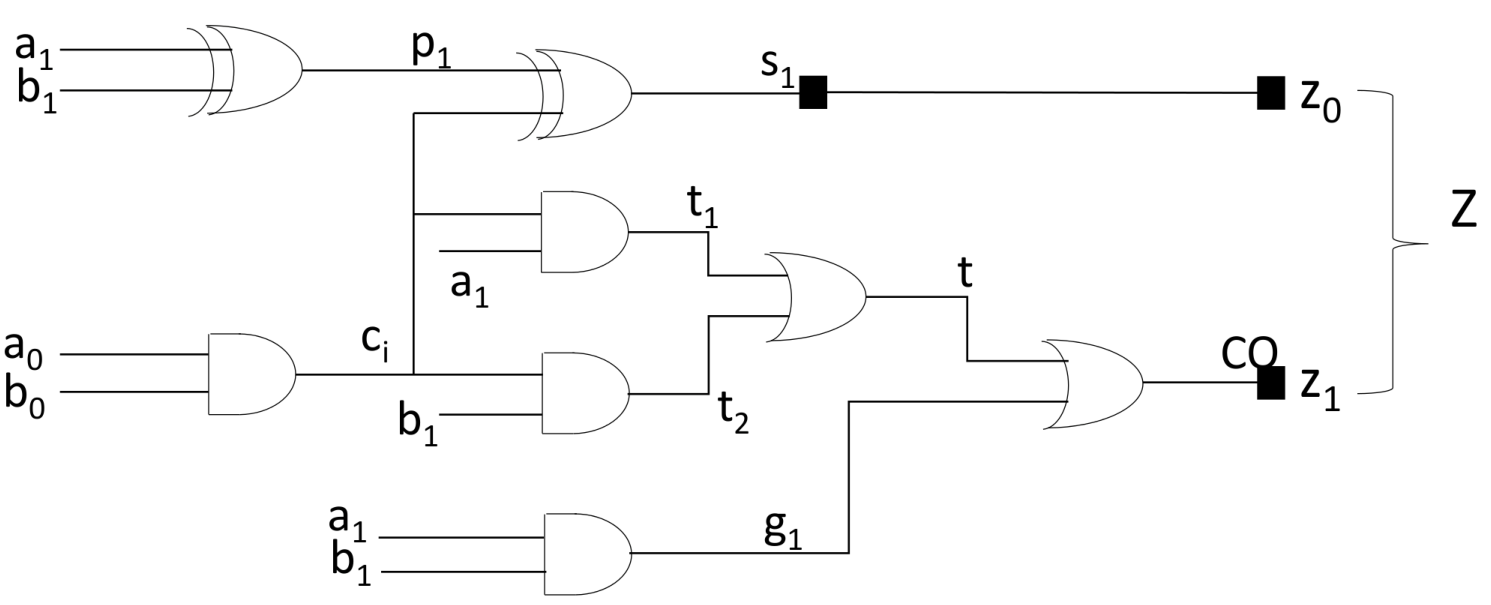
\includegraphics[width=\textwidth]{newfig/tobemapped.pdf}
	\end{center}
	\caption{An example gate-level netlist to be mapped}
	\label{fig:tobemapped}
\end{figure}

Figure \ref{fig:tobemapped} shows an example circuit partition with $a_1,b_1,a_0,b_0$ as inputs and
$Z = \{z_0,z_1\}$ as outputs. If we use elements from Galois field $\F_{2^2}$ to represent word $Z$,
we have $Z = z_0 + \alpha\cdot z_1$.

After imposing ATO of LEX with
$$Other\ circuit\ variables > output\ word\ Z > all\ bit\ level\ inputs$$
on the ideal describing the partitioned circuit as well as ideal with vanishing polynomials,
the reduced Gr\"obner basis has a single polynomial generator in the form of $Z + \Func(a_1,b_1,a_0,b_0)$.
In this example:

\begin{itemize}
\item Term ordering: $\{z_0,z_1,t,g_1,p_1,ci,t_1,t_2\}>Z>\{a_0,b_0,a_1,b_1$
\item Gate description: $z_0+t+g_1+t\cdot g_1, t+t_1+t_2+t_1\cdot t_2, g_1+a_1\cdot b_1,
			t_1+a_1\cdot ci, t_2+b_1\cdot ci, ci+a_0\cdot b_0, z_1+p_1+ci, p_1+a_1+b_1$
\item Word definition: $Z+z_0+z_1\cdot \alpha$
\item Vanishing polynomial ideal $(J_0)$: $z_0^2+z_0, z_1^2+z_1, t^2+t, g_1^2+g_1, t_1^2+t_1, t_2^2+t_2, p_1^2+p_1, ci^2+ci,
			a_0^2+a_0, b_0^2+b_0, a_1^2+a_1, b_1^2+b_1, Z^4+Z$(since Z is a 2-bit word)
\end{itemize}

The result is a Gr\"obner basis with single polynomial generator. The polynomial has leading term $Z$:
$$Z+a_0\cdot b_0\cdot a_1+a_0\cdot b_0\cdot b_1+\alpha\cdot a_0\cdot b_0+a_1\cdot b_1+\alpha\cdot a_1+\alpha\cdot b_1$$

% \begin{table}
% \centering
% \begin{tabular}{|c|c|} \hline
% Boolean operator & operation in $\mathbb{F}_{2}$\\ \hline
% $\overline{a}$ & $1 + a$\\ \hline
% $a\ and\ b$ & $ab$\\ \hline
% $a\ or\ b$ & $a + b + ab$\\ \hline
% $a \oplus b$ & $a + b$\\
% \hline\end{tabular}
% \caption{Some Boolean operators and corresponding operations in $\mathbb{F}_{2}$}
% \label{table:booltogalois_op}
% \end{table}

2) {\bf Templates on Boundary Information:}
\begin{figure}[h]
	\begin{center}
	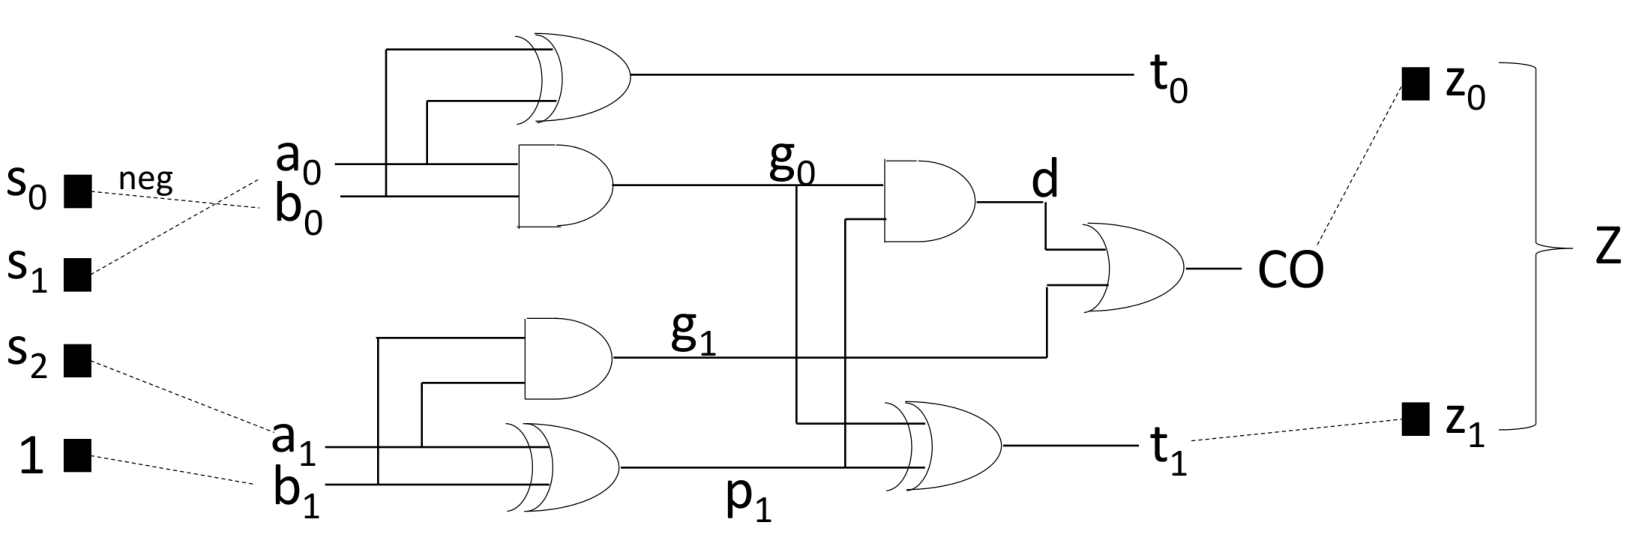
\includegraphics[width=\textwidth]{newfig/template.pdf}
	\end{center}
	\caption{Standard 2-bit adder with input/output mapping}
	\label{fig:template}
\end{figure}

Figure \ref{fig:template} shows a 2-bit standard cell. It has 3 outputs mapped to 2 output pins,
and 4 inputs mapped to 3 input pins (the rest pins are assigned to fixed 0/1 signal). Dashed connection
lines show one possible mapping, to find out this kind of feasible mapping, we need to simulate
all possible mappings, where the concept "template" can be used.

{\it Output template}: $z_0+c_{{t_0}{z_0}}\cdot t_0+c_{t_1z_0}\cdot t_1+c0_{CO}\cdot CO+c_{n_0}$

When $c_{n_0} = 0$, then $\{c_{t_0z_0},c_{t_1z_0},c0_{CO}\}$ equals to 1 denotes a valid mapping to corresponding output pin. 
Conversely if $cn0 = 1$, the ``1" evaluation denotes mapping to negation of corresponding output pin.

{\it Input template}: $a_0+p_{a_0}+c0_{A_0}\cdot s_0+c1_{A_0}\cdot s_1+c2_{A_0}\cdot s_2$

When $p_{a_0} = 0$, then $\{c0_{A_0},c1_{A_0},c2_{A_0}\}$ equal to 1 denotes a valid mapping to corresponding input
pin. Conversely if every variable in set $\{c0_{A_0},c1_{A_0},c2_{A_0}\}$ equals to 0, it denotes mapping to fixed signal ``0" (when $p_{a_0} = 1$ then
mapping to fixed signal ``1").

With these settings, we propose an approach to perform technology mapping with boundary information:
\begin{itemize}
\item First, choose a set of independent wires as input pins;

\item Second, push forward input signal for a certain number of gates (depth), choose a cut set
which fully dependent on these inputs as output pins;

\item Third, abstract a description polynomial using GB based abstraction;

\item Fourth, reduce the description polynomial with the GB we computed associated to macro block 
and templates, obtain a remainder polynomial;

\item Last but not least, abstract all coefficients from the remainder polynomial and set up a system of equations.
If we find a solution to this system, then the solution is a feasible mapping; no solution means we cannot make a
feasible mapping.
\end{itemize}

\numberofappendices=1
\appendix
\chapter{}
\fixchapterheading
\section{Normal Basis Theory}
\label{append:NB}
\subsection{Characterization of Normal Basis}
\subsection{Construction of General Normal Basis}
\subsection{Bases Conversion}
% General \lambda matrix computation

\section{Optimal Normal Basis}
\label{append:ONB}
\subsection{Construction of Optimal Normal Basis}
\subsection{Optimal Normal Basis Multiplier Design}
% Customized Galois Field IEEE1363-2000
% Multi table <=> \lambda matrix

%\newpage

%%%%%%%%%%%%%%%%%%%% The bibliography %%%%%%%%%%%%%%%%%%%%%%%%%%%%

\bibliographystyle{ieee}
\bibliography{logic,xiaojun,cnfsat}
\end{document}

%%%%%%%%%%%%%%%%%%%%%%%%%%%  End of IEEEsample.tex  %%%%%%%%%%%%%%%%%%%%%%%%%%%
